\begin{singlespacing}
\chapter{A search for new phenomena}
\label{chapter:2ljets}
%
\begin{epigraphs}
\qitem{%
An experiment is never a failure solely because it fails to
achieve predicted results. An experiment is a failure only when it also
fails adequately to test the hypothesis in question, when the data it
produces don’t prove anything one way or another.%
}%
{Robert~M.~Pirsig,
\emph{Zen and the Art of Motorcycle Maintenance},
1974~\cite{pirsig1999zen}}
\qitem{%
But there is one feature I notice that is generally missing in cargo cult
science. \ldots\
% That is the idea that we all hope you have learned in studying science in
% school --- we never say explicitly what this is, but just hope that you catch
% on by all the examples of scientific investigation. It is interesting,
% therefore, to bring it out now and speak of it explicitly.
It's a kind of scientific integrity, a principle of scientific thought that
corresponds to a kind of utter honesty --- a kind of leaning over backwards.%
}%
{Richard~Feynman,
\emph{Cargo Cult Science},
1974~\cite{feynman1974cargo}}
\end{epigraphs}
\end{singlespacing}

My core contributions in this thesis are to the recent \atlas\
searches ``for new phenomena in events with two leptons, jets, and
missing transverse momentum''~\cite{atlas2022searches},
particularly to its electroweak part.
For brevity, I will call this publication $\twoljets$ and its electroweak
subset $\twoljets$-electroweak.

This chapter follows a questionable order.
It may be clearer, and is certainly more ordinary,
to first present preparations (blind to data),
followed later by the results (unblinded).
Instead, this chapter first reports the unblinded results, then follows with
in-depth discussions of individual elements, partially in light of those
results.
I choose this order for two reasons.
Firstly, it avoids iterating over those elements twice, once before and again
after unblinding.
The analysis has many little and loosely related pieces that I attempt to
to cover locally to reduce jumps between far-flung corners of the
chapter.
Secondly, and sadly, many design decisions can only be explained in light of the
unblinded results, since important aspects were reworked in the
nineteen months between its unblinding and eventual publication.

There are certain plots and tables which, personally, I first seek when
meeting an \atlas\ search paper, particularly the summary plot with all signal
regions and the model-dependent exclusion contours.
This chapter begins by presenting those results in brief in Section
~\ref{sec:2ljets_splash}.
The meat of the chapter follows.
\begin{itemize}
\item Context from previous searches and inspirations for the design goals
of the $\twoljets$-electroweak search are described in
Section~\ref{sec:2ljets_context}.
\item Data, their event variables and the reconstructed objects from which
they derive are described in Section~\ref{sec:2ljets_events}.
\item Region design for the $\twoljets$-electroweak search is described and
explained in Section~\ref{sec:2ljets_design}.
\item The modelling of our uncertain predictions of background and signal
contributions in those regions is covered in
Section~\ref{sec:2ljets_modelling}.
\item Some validation studies are presented in
Section~\ref{sec:2ljets_validation}.
\item The unblinding procedure of this search is discussed in
Section~\ref{sec:2ljets_unblinding}, and
\item and some additional results are presented in
Section~\ref{sec:2ljets_results}.
\TODO{Conclusions}
\end{itemize}


\subsection{Splash summary}
\label{sec:2ljets_splash}
% begin with physics content and results
Unblinded results in all main regions of the $\twoljets$-electroweak analysis
are presented in of the Figure~\ref{fig:2ljets_summary}.
Since this figure appears to represent the data and background estimates,
on which all derived results depend, it could be seen as the keystone of this
thesis.
There are, however, caveats to be developed later in this chapter.

In numerous orthogonal signal regions, no significant excess is observed
above \emph{post-fit} backgrounds.
Indeed, there are some significant deficits --- data below the background noise.

Background parts of a \heplikelihood\ model are illustrated behind data.
To test non-standard (supersymmetric) models against observation, signal
contributions are added on top of those backgrounds.

We use two signal models in the $\twoljets$-electroweak analysis.
One is an MSSM chargino-neutralino model (C1N2) which acts to produce
$\chargino_1\textrm{--}\neutralino_2$ pairs, which decay via
$W\rightarrow q\bar q$ and
$Z\rightarrow \ell^\pm \ell^\mp$ respectively.
The other is a GMSB model which, from a variety of initial states, produces
$\neutralino_1\textrm{--}\neutralino_1$ pairs.
These neutralinos decay,
via Higgs and $Z$ bosons in variable branching fractions,
to final states again containing $\ell^\pm \ell^\mp$ and jet-seeding partons.
Diagrams illustrating these C1N2 and GMSB signal models are shown in
Figure~\ref{fig:2ljets_signal_diagrams}.

Effects of some of these signals in example signal regions of the
$\twoljets$-electroweak analysis are displayed in
Figure~\ref{fig:2ljets_signal_examples}.

At each parameter point of a signal model, it is added to the background model
and tested against data in the $\cls$ prescription.
Contours showing which parameters of those signal models are labelled as
excluded are displayed for
C1N2 in Figure~\ref{fig:2ljets_contours_c1n2} and for
GMSB in~\ref{fig:2ljets_contours_gmsb}.

Data in discovery regions are presented and interpreted in
Table~\ref{tab:2ljets_discovery}.

% summary plot
\begin{figure}[tp]
\centering
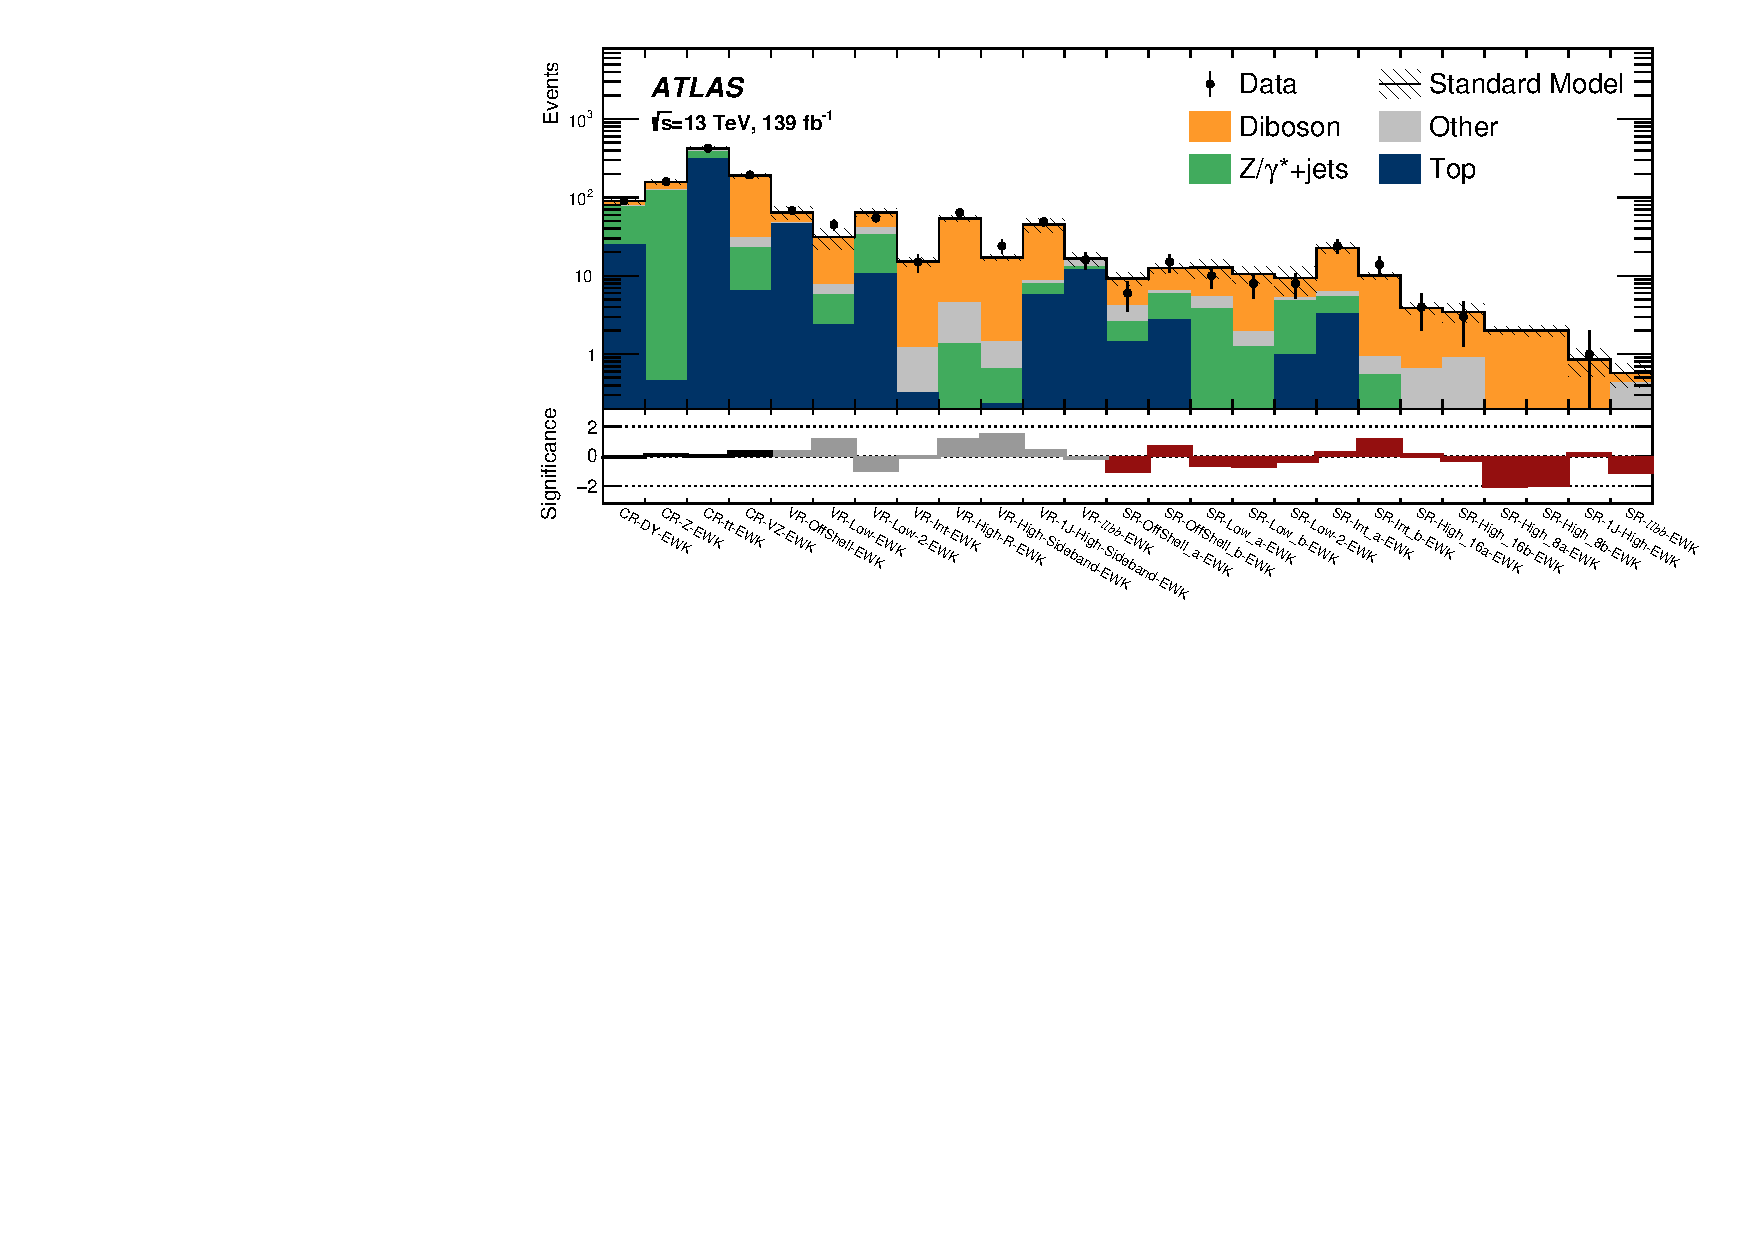
\includegraphics[width=\textwidth]{figures/2ljets_summary_log.pdf}
\caption[
Data of the $\twoljets$-electroweak analysis with \emph{post-fit}
backgrounds
]{%
Data of the $\twoljets$-electroweak analysis with \emph{post-fit}
backgrounds~\cite{atlas2022searches}.
The lower panel shows $S_\mathrm{ATLAS}$ from
Equation~\ref{eqn:significance_atlas}.
Control, validation and signal regions are shown from left to right, with the
regions within each category ordered approximately by their typical $\met$.
Likelihoods from validation regions are not included in the fit.
The `Top' category contains $\ttbar$ and $tW$ processes, and
`Other' contains fake/non-prompt lepton, higgs, triboson, $\ttbar Z$, and other
\topother\ processes.%
}
\label{fig:2ljets_summary}
\end{figure}

% signal diagrams
\begin{figure}[t]
\centering
\begin{subfigure}{0.48\textwidth}
\centering
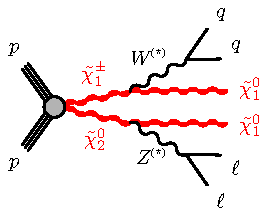
\includegraphics[width=\textwidth]{figures/2ljets_c1n2_llqqn1n1_wz.pdf}
\caption{C1N2}
\end{subfigure}
\hfill
\begin{subfigure}{0.48\textwidth}
\centering
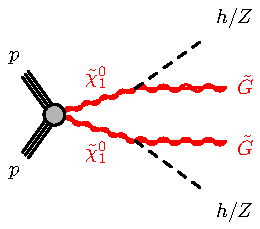
\includegraphics[width=\textwidth]{figures/2ljets_n1n1_hhggzz.pdf}
\caption{GMSB}
\end{subfigure}
\caption[
Supersymmetric signal processes in the $\twoljets$-electroweak analysis
]{%
Supersymmetric signal processes in the $\twoljets$-electroweak analysis.
\emph{Figures are reproduced from the paper%
}~\cite{atlas2022searches, atlas_susy_feynman}.
\\[0.5em]
(a): C1N2, where the initial $\chargino_1\textrm{--}\neutralino_2$ pair
is produced through a $s$-channel $W^{\pm}$ resonance and the masses of
weak bosons in decays are bounded by the mass splitting
$m(\chargino_1, \neutralino_2) - m(\neutralino_1)$.
We explore the parameters
$m(\chargino_1, \neutralino_2)$ and $m(\neutralino_1)$.
\\[0.5em]
(b): GMSB, where the initial $\neutralino_1\textrm{--}\neutralino_1$ pair
is produced by soft decays from pairs including $\chargino_1$,
$\neutralino_2$ or $\neutralino_1$.
Although the $h$ and $Z$ bosons decay to many states, we target
$Z\rightarrow \ell\ell$ with
$h/Z\rightarrow bb/jj$.
We explore the parameters
$m(\neutralino_1)$ and $B(\neutralino_1 \rightarrow h \tilde{G})$ with fixed
$m(\chargino_1, \neutralino_2) - m(\neutralino_1) = 1\,\eV[G]$.
}
\label{fig:2ljets_signal_diagrams}
\end{figure}

% signal region plots
\begin{figure}[tp]
\centering
\begin{subfigure}{0.48\textwidth}
\centering
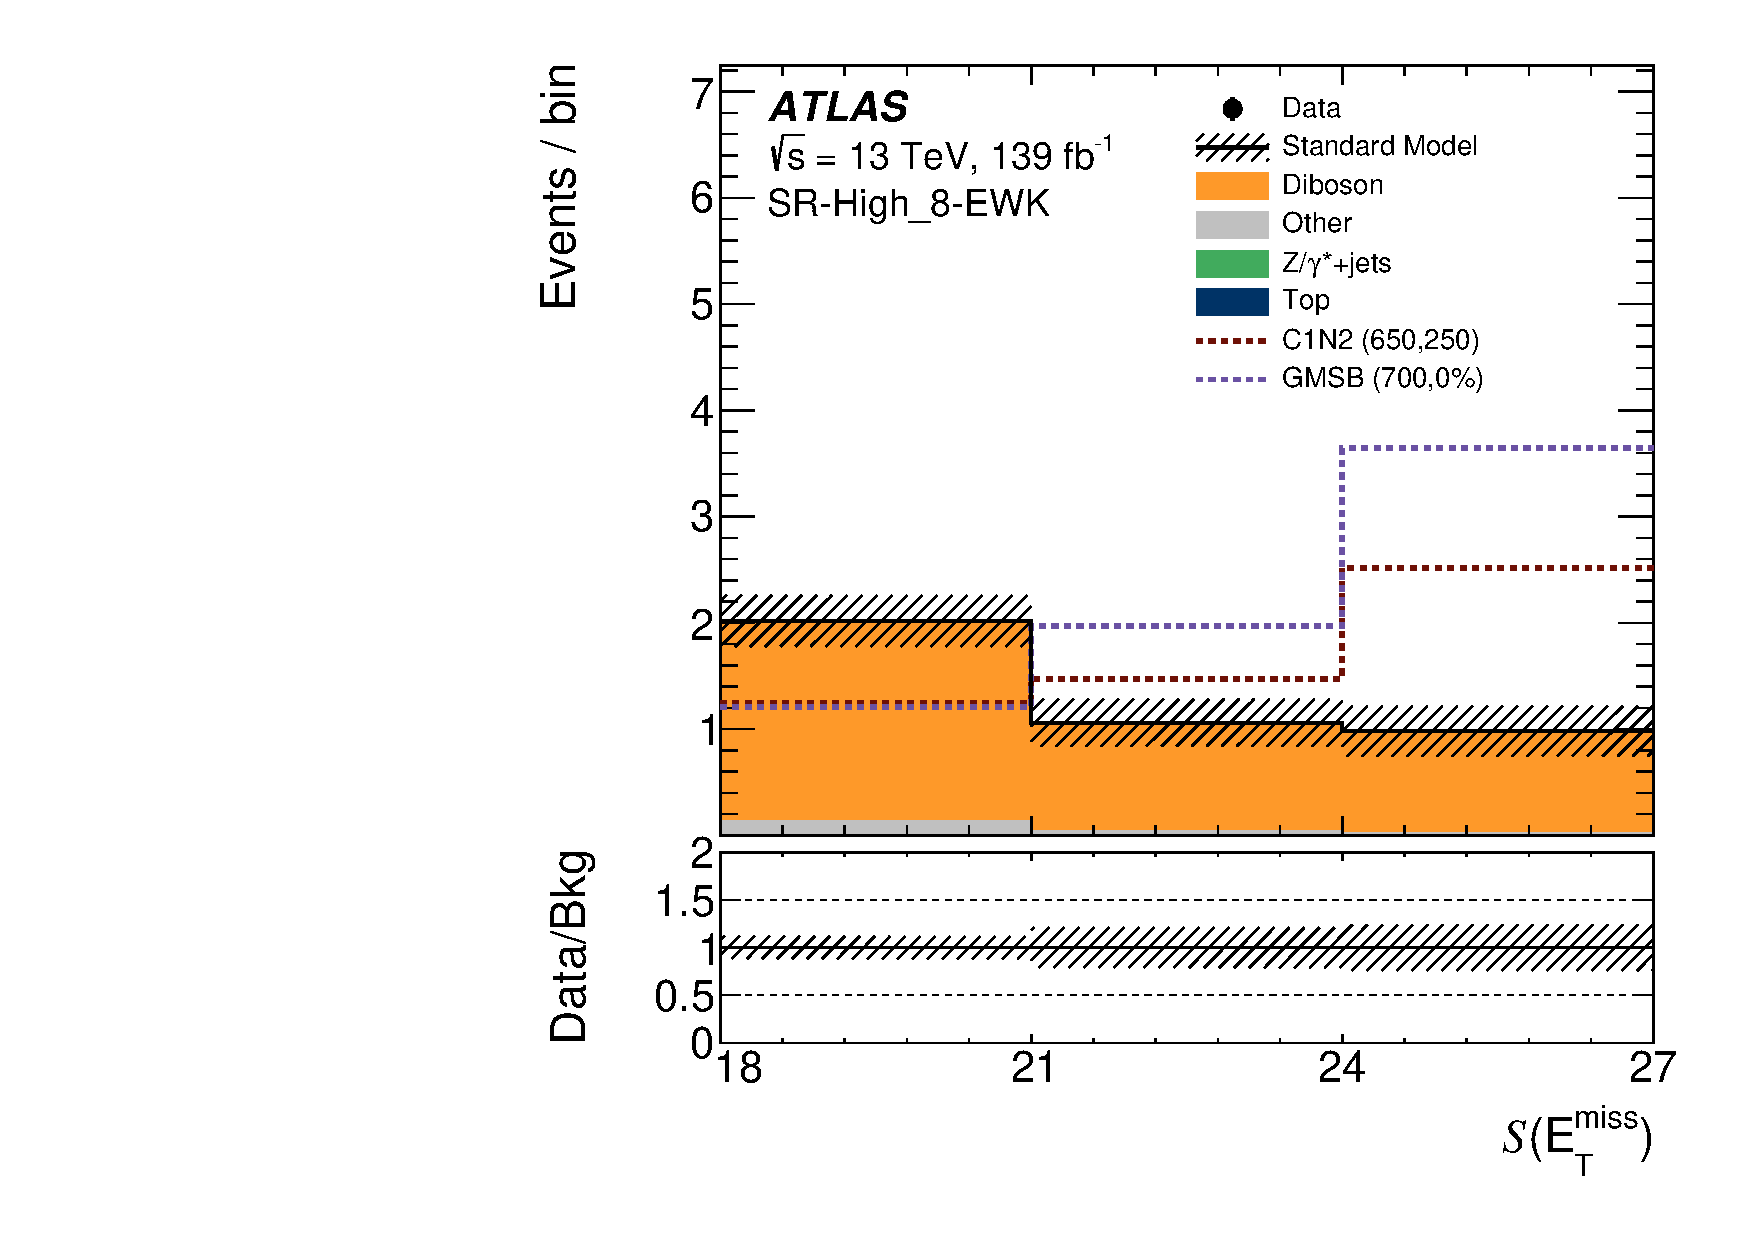
\includegraphics[width=\textwidth]{figures/2ljets_sr_high_8_met_sig.pdf}
\caption{SR-High-8}
\end{subfigure}
\hfill
\begin{subfigure}{0.48\textwidth}
\centering
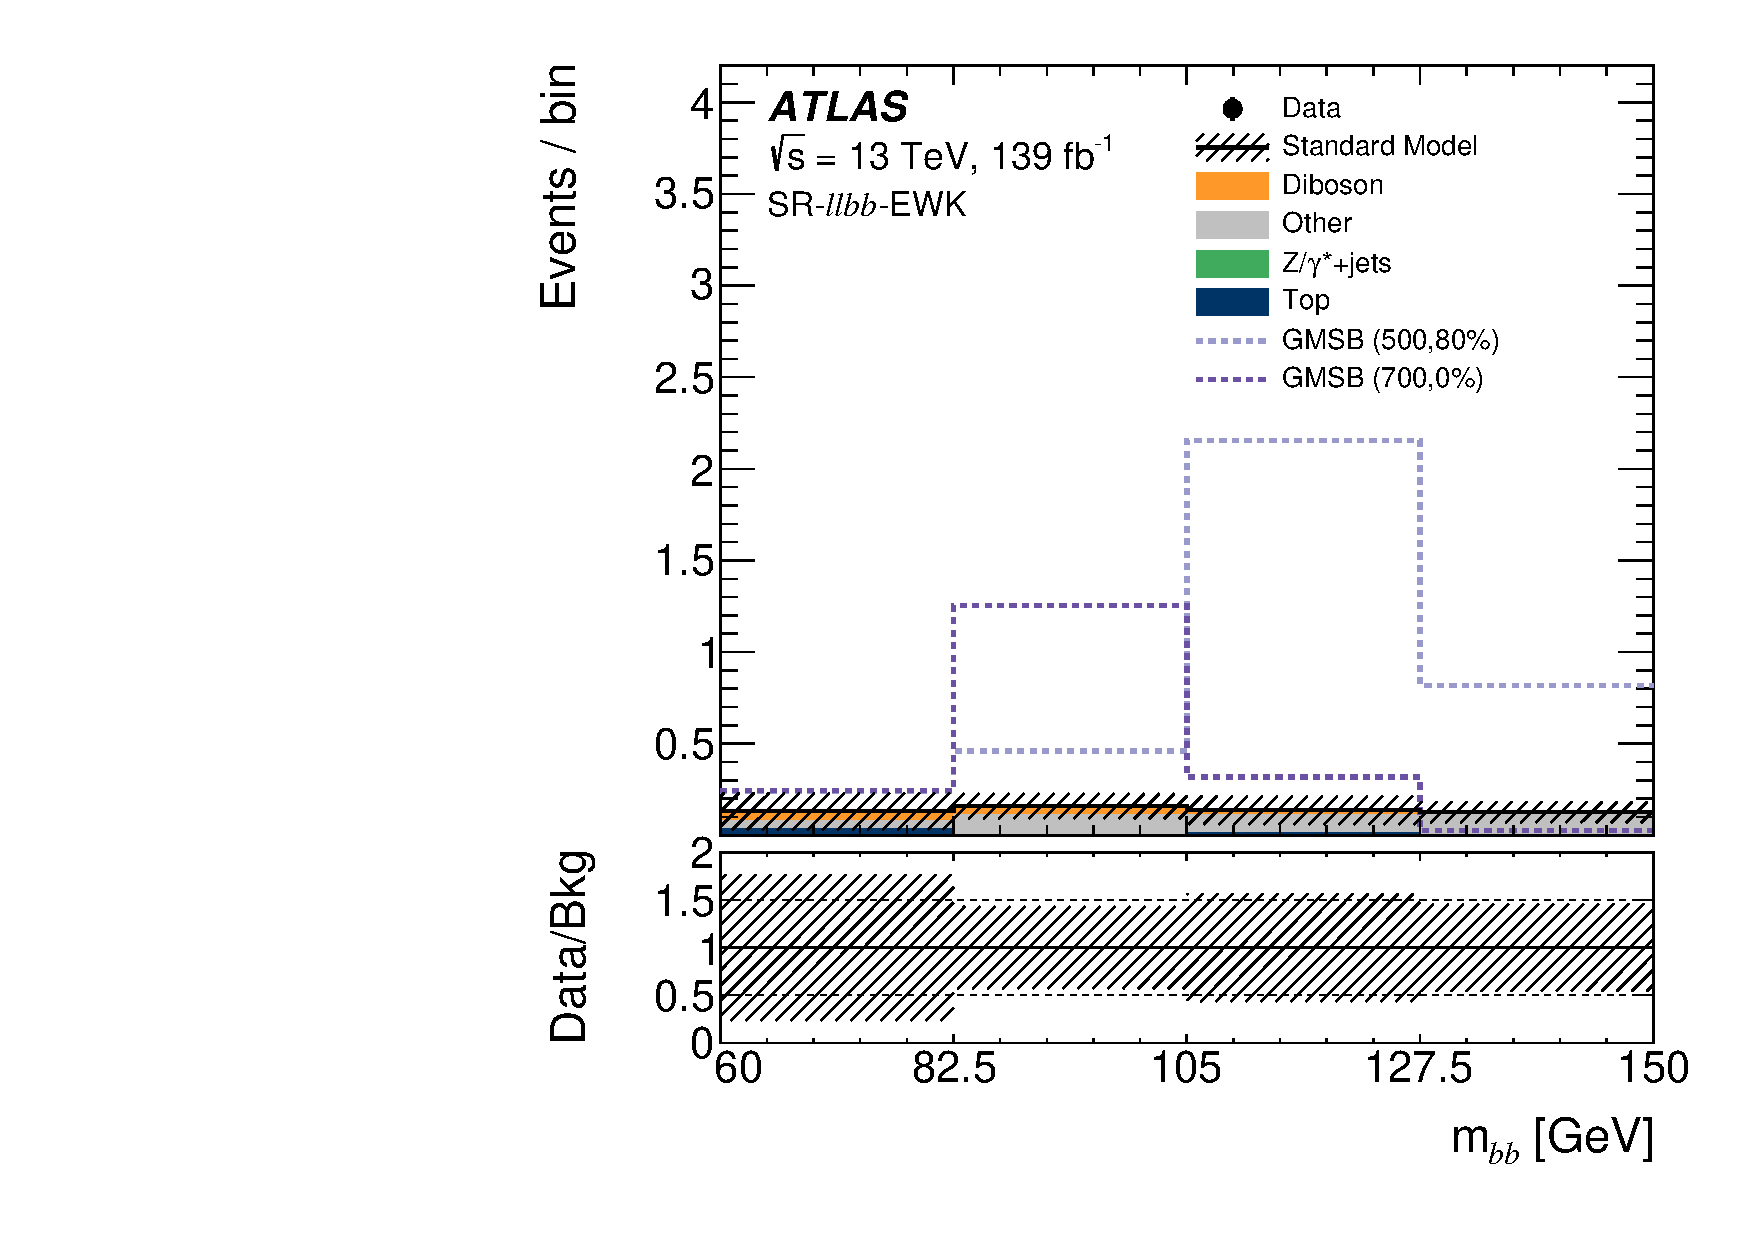
\includegraphics[width=\textwidth]{figures/2ljets_sr_llbb_mbb.pdf}
\caption{\srllbb}
\end{subfigure}
\\[0.5em]
\begin{subfigure}{0.48\textwidth}
\centering
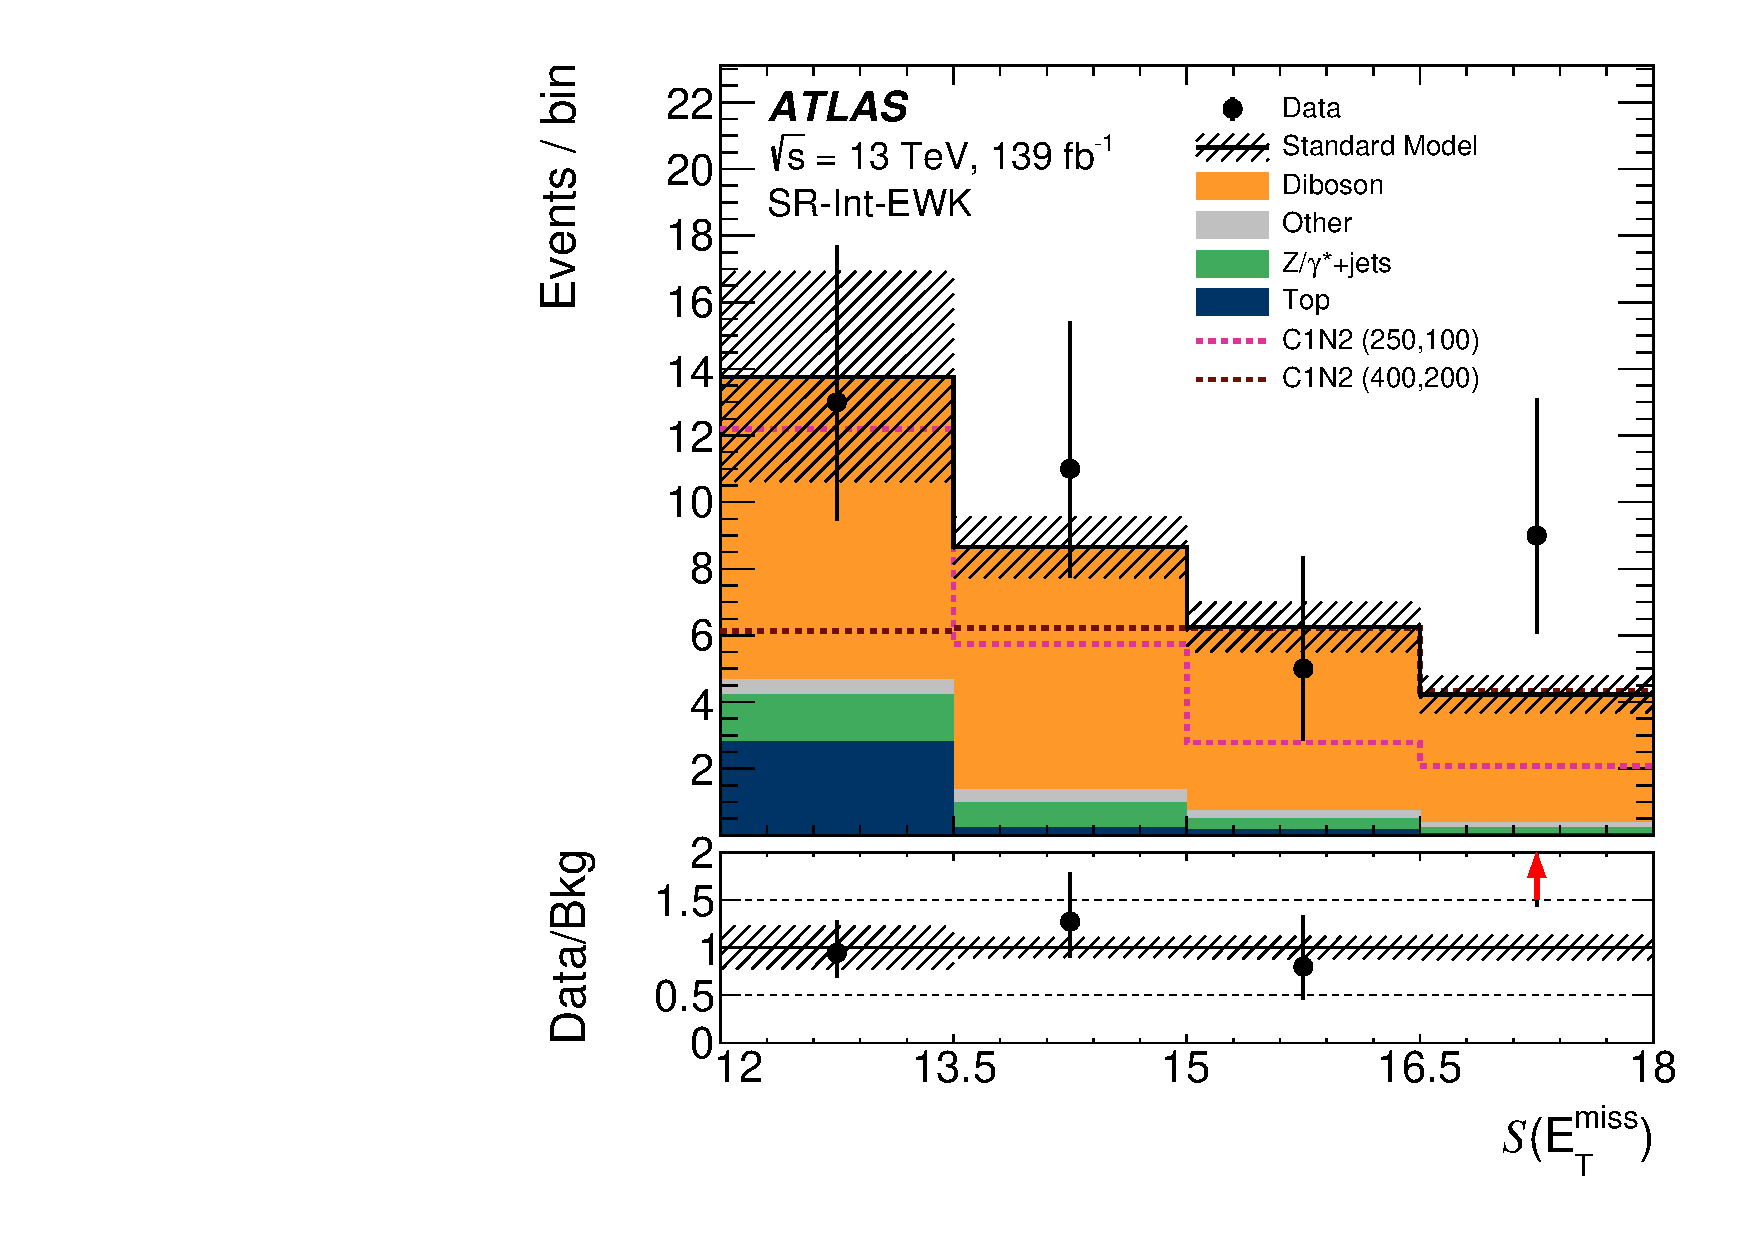
\includegraphics[width=\textwidth]{figures/2ljets_sr_int_met_sig.pdf}
\caption{SR-Int}
\end{subfigure}
\hfill
\begin{subfigure}{0.48\textwidth}
\centering
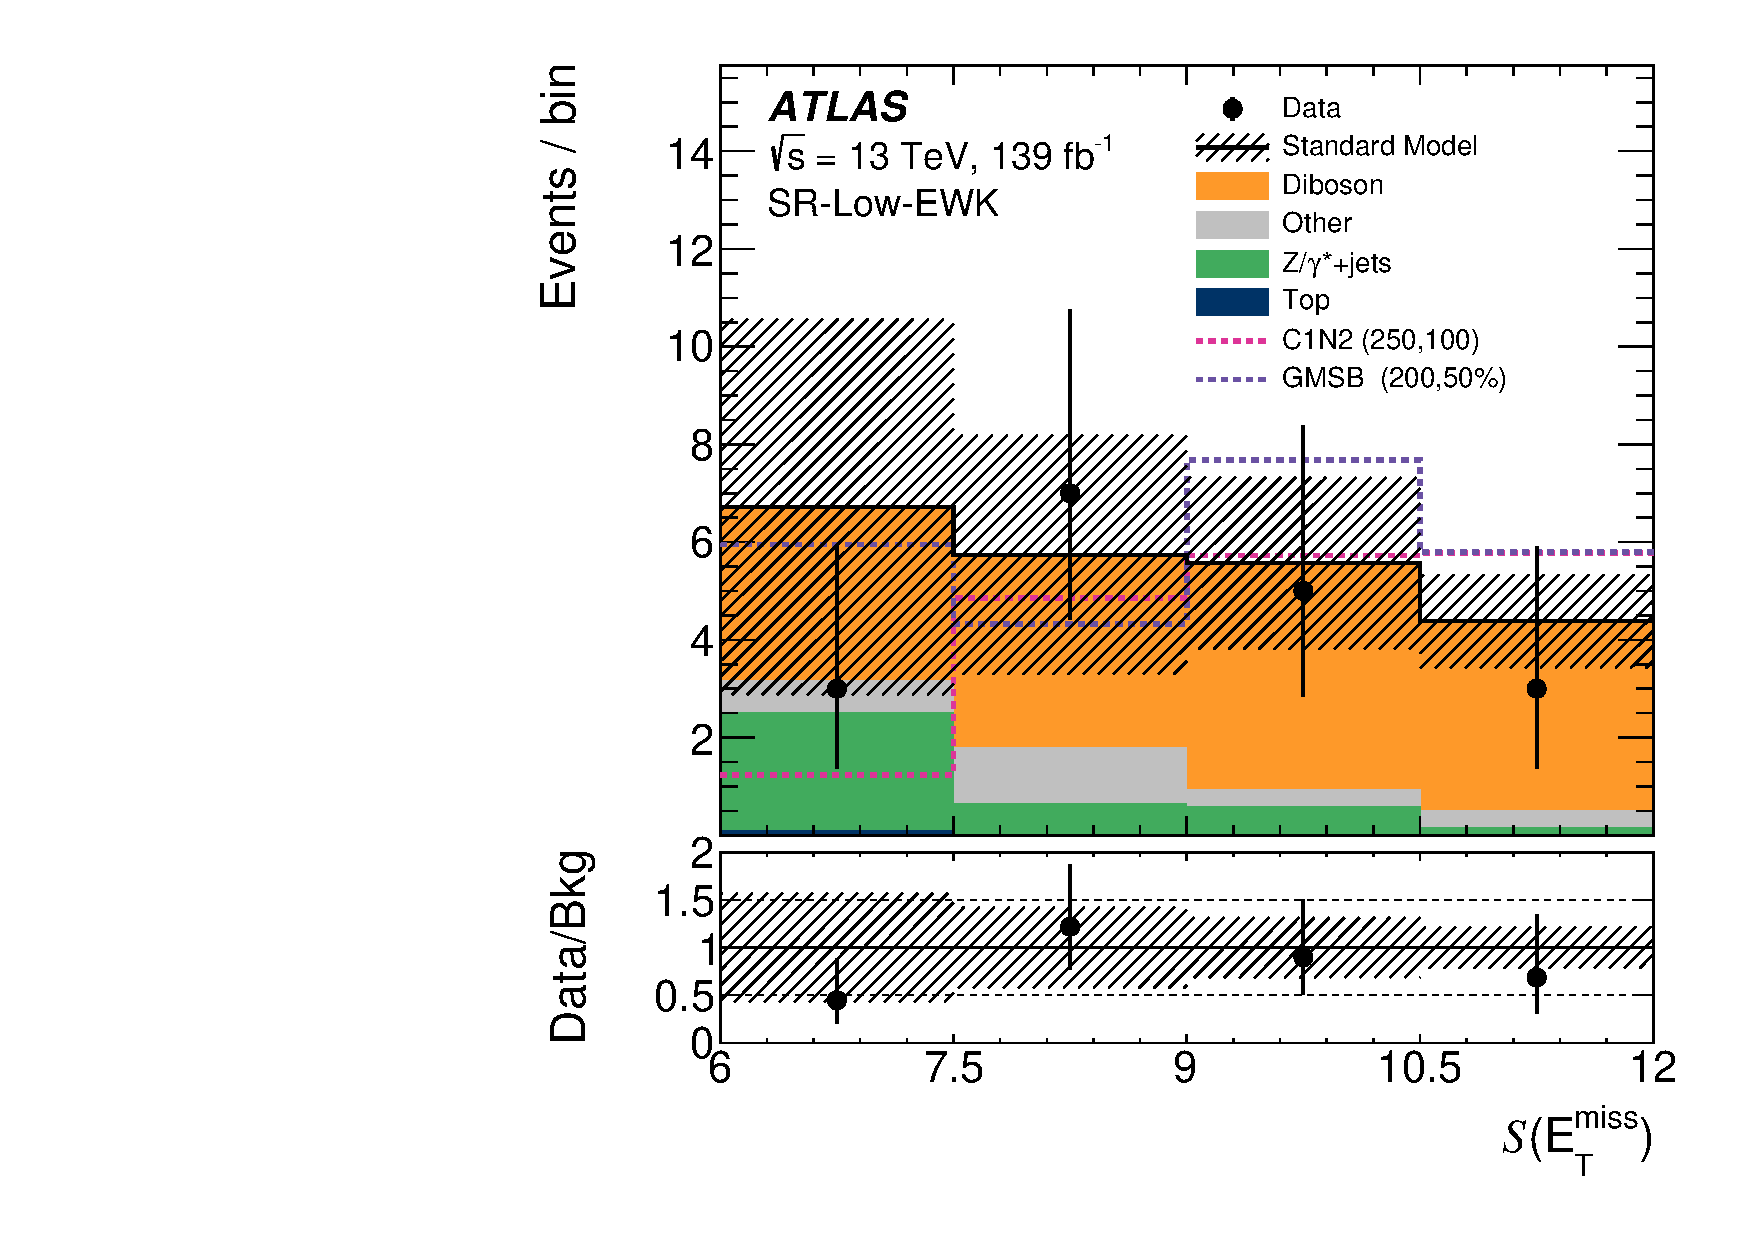
\includegraphics[width=\textwidth]{figures/2ljets_sr_low_met_sig.pdf}
\caption{SR-Low}
\end{subfigure}
\caption[
Example signal region histograms with benchmark signal sample yields overlaid
]{%
Example signal region histograms with benchmark signal sample yields overlaid
as dotted lines~\cite{atlas2022searches}.
Physically, signal yields would add on top of the backgrounds.
Data are shown; regions in the top two plots observe zero data, and
Poisson error bars for zero events are hidden for aesthetic reasons.
}
\label{fig:2ljets_signal_examples}
\end{figure}

% exclusion plots
\begin{figure}[tp]
\centering
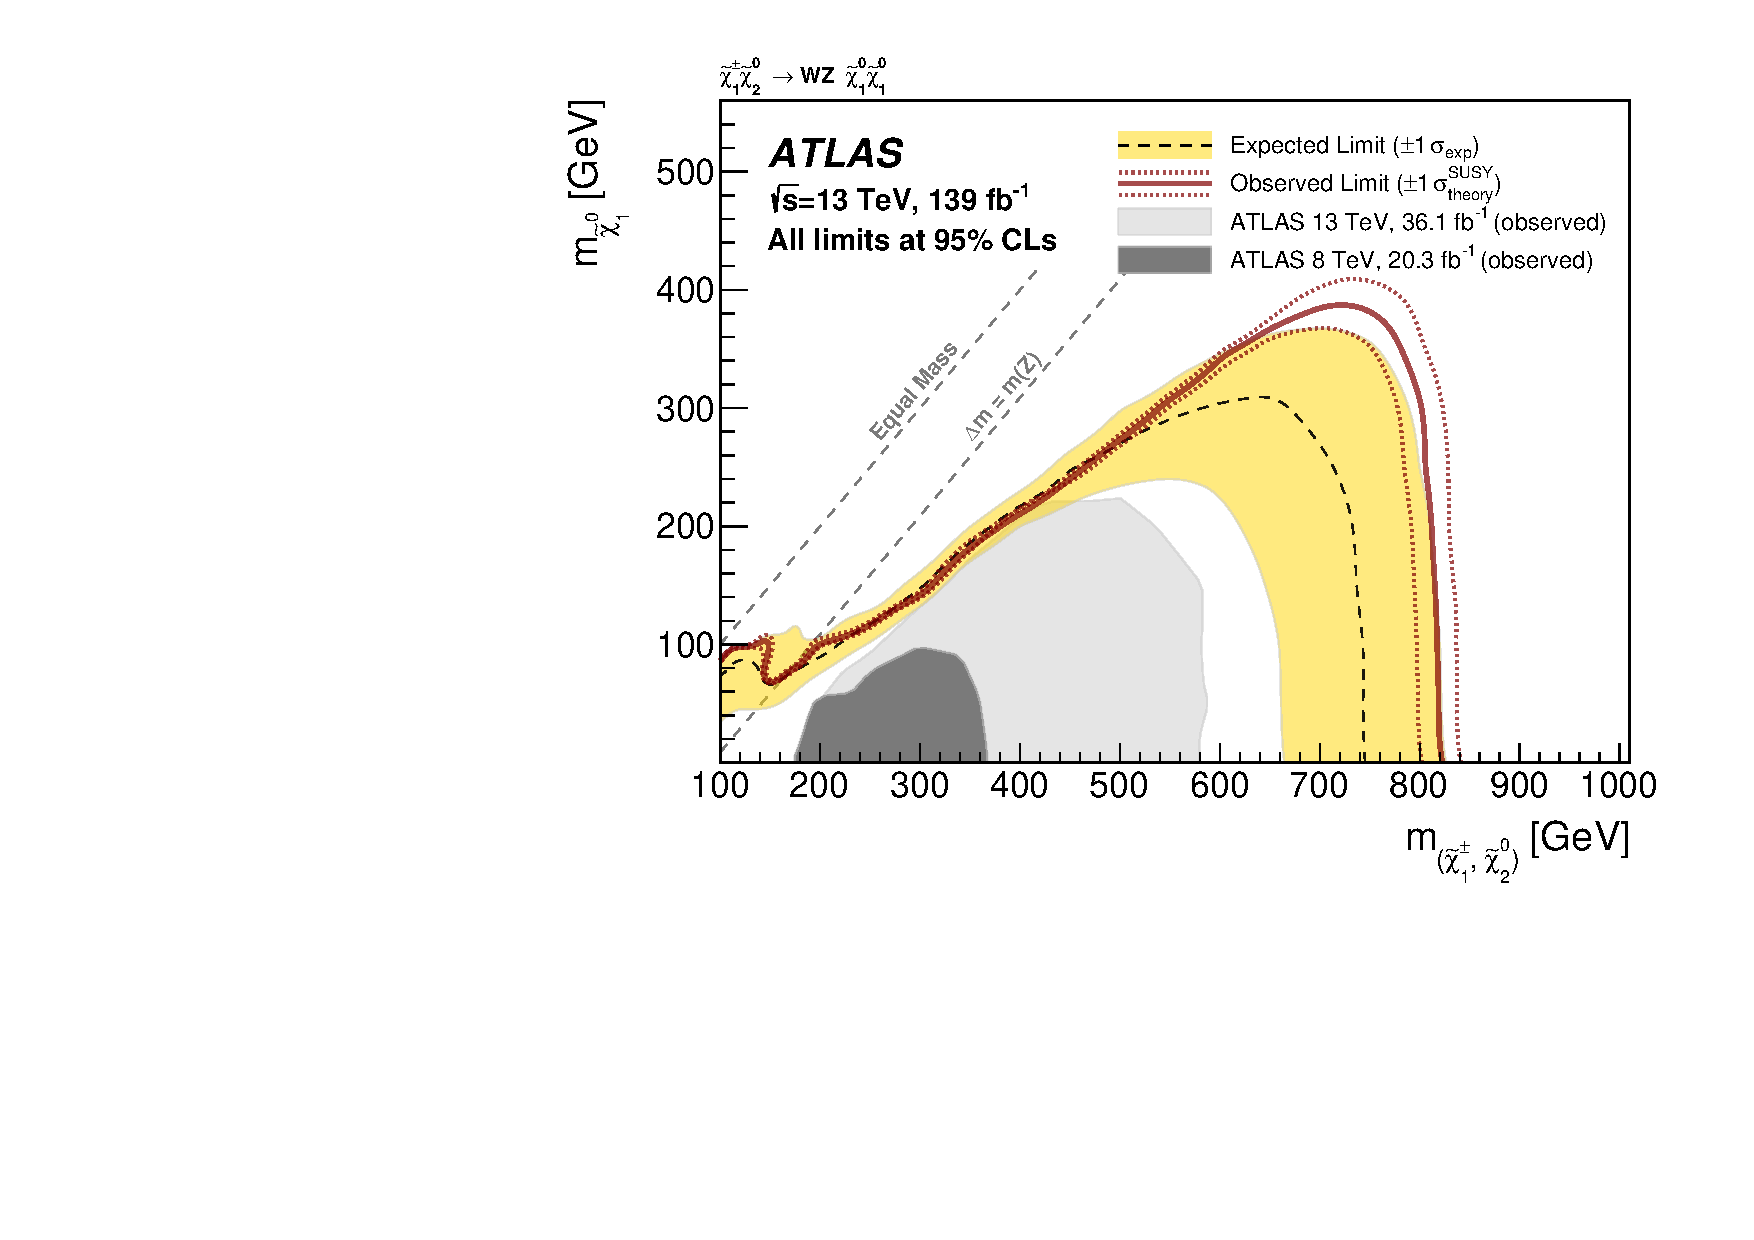
\includegraphics[width=0.99\textwidth]{figures/2ljets_contours_c1n2.pdf}
\caption[
Contours for the C1N2 model in the $\twoljets$-electroweak analysis
]{%
Contours for the C1N2 model in the $\twoljets$-electroweak
analysis~\cite{atlas2022searches}.
\\[0.5em]
Space below the solid red line is labelled as excluded, and its dotted
neighbours show the result if all signal cross-sections are varied up and down
by theoretical error bars.
\\[0.5em]
The yellow band shows the $\pm1$-sigma region of exclusion contours
from asymptotic approximations to the prior distribution of the test statistic.
Grey areas are observed limits from the two-lepton parts
of~\cite{atlas_23l_SUSY_2016_24} and~\cite{atlas_2l_SUSY_2013_11}.
Exclusion is defined by the $95\%$ $\cls$ prescription
in asymptotic approximations.
All contours are interpolated from a sparse grid.
}
\label{fig:2ljets_contours_c1n2}
\end{figure}

\begin{figure}[tp]
\centering
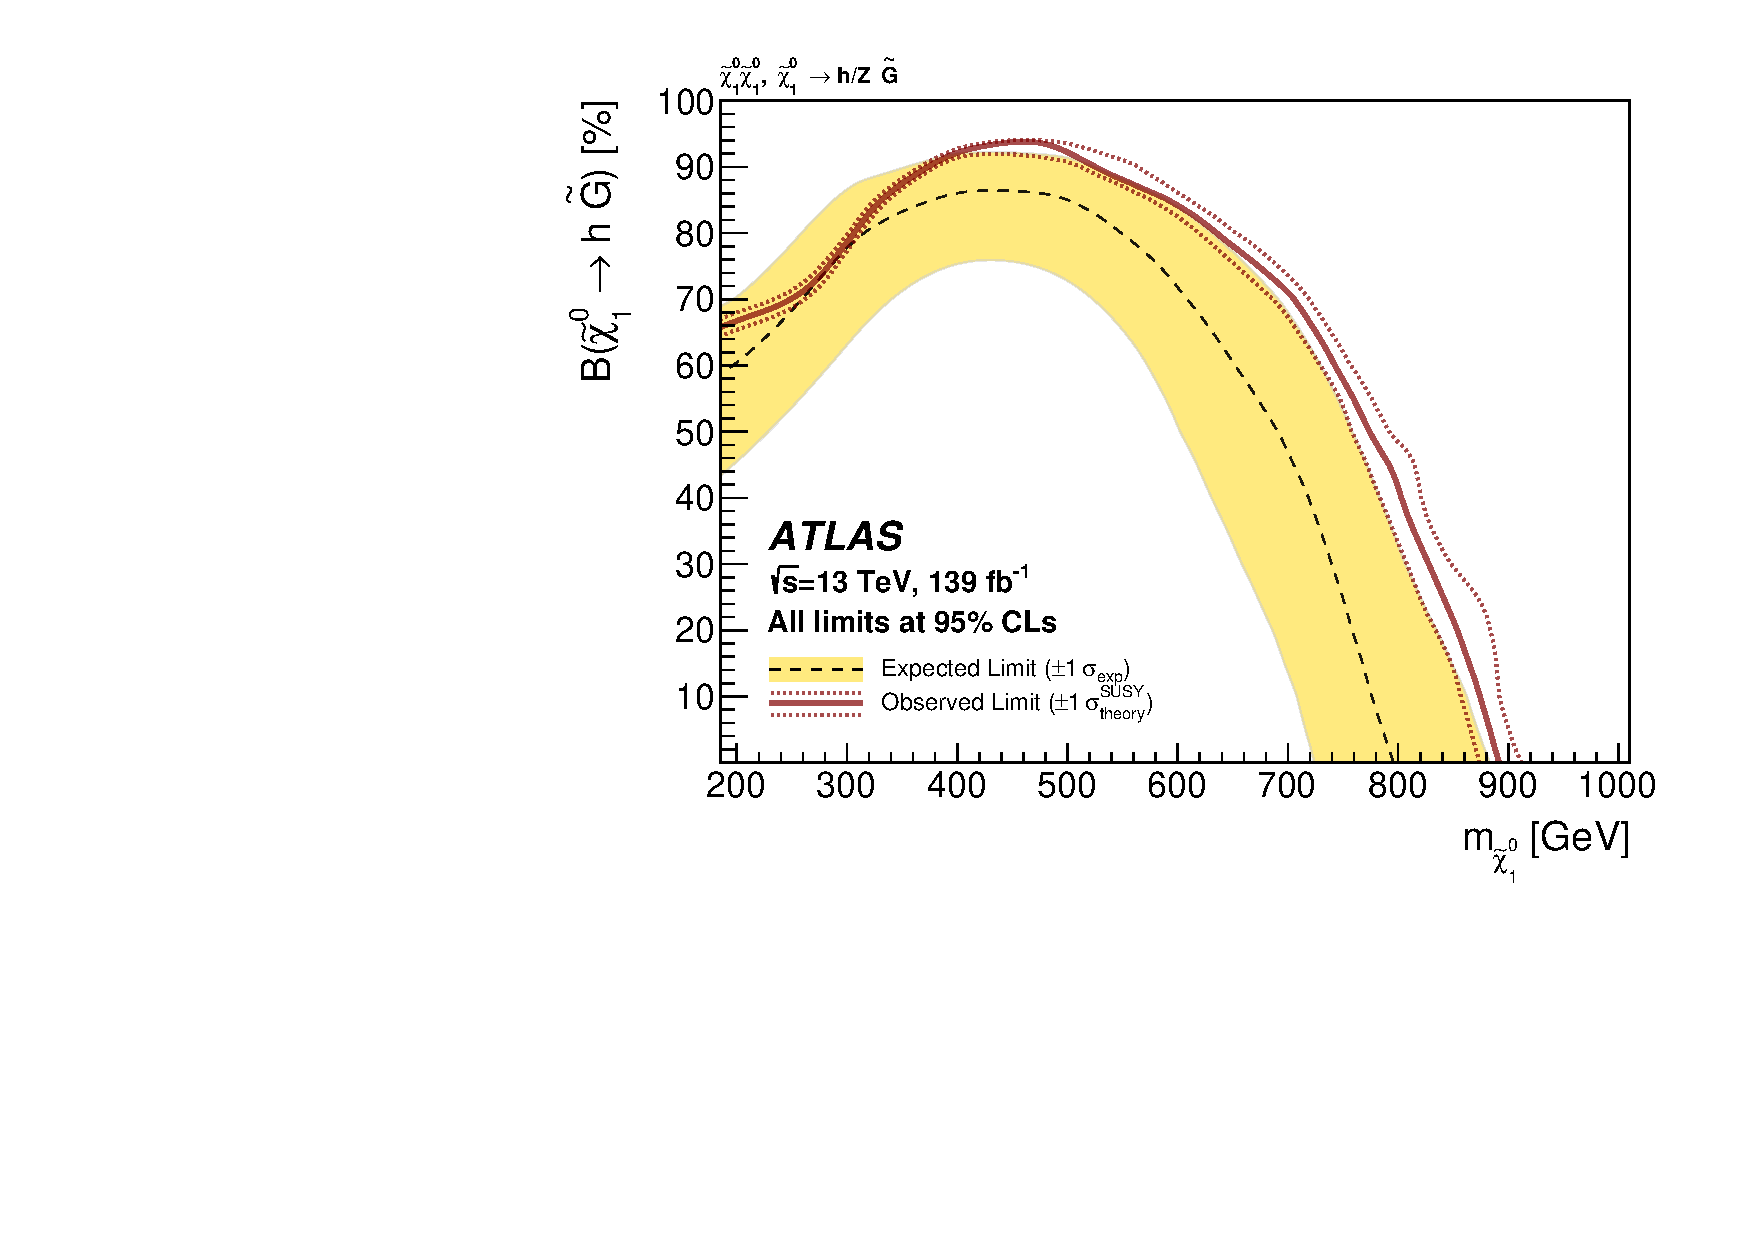
\includegraphics[width=0.99\textwidth]{figures/2ljets_contours_gmsb.pdf}
\caption[
Contours for the GMSB model in the $\twoljets$-electroweak analysis
]{%
Contours for the GMSB model in the $\twoljets$-electroweak
analysis~\cite{atlas2022searches}.
\\[0.5em]
Space below the solid red line is labelled as excluded, and its dotted
neighbours show the result if all signal cross-sections are varied up and down
by theoretical error bars.
\\[0.5em]
The yellow band shows the $\pm1$-sigma region of exclusion contours
from asymptotic approximations to the prior distribution of the test statistic.
Exclusion is defined by the $95\%$ $\cls$ prescription
in asymptotic approximations.
All contours are interpolated from a sparse grid.
}
\label{fig:2ljets_contours_gmsb}
\end{figure}

% upper limits
% definitely want this after pictures
\FloatBarrier
\begin{table}[tp]
\centering
% custom separator for aligned +-
% https://stackoverflow.com/a/2132998
\begin{tabular*}{\textwidth}{lr@{$~\pm~$}lcccccc}
& \multicolumn{2}{c}{Fitted}
& Data
& $A\epsilon\sigma_{\mathrm{obs}}^{95}~\mathrm{fb}$
& $S_{\mathrm{obs}}^{95}$
& $S_{\mathrm{exp}}^{95}$
& $\clb$
& $p_{s\!=\!0}$
\\[1.5ex]
DR-OffShell & $22.1$ & $2.7$ & $21$ & $0.10$ & $14.3$ & $12.3^{+4.7}_{-3.1}$ & $0.68$ & $0.50$
\\[.5ex]
DR-Low & $22$ & $4$ & $18$ & $0.08$ & $10.8$ & $15.3^{+5.7}_{-4.0}$ & $0.09$ & $0.50$
\\[.5ex]
DR-Int & $35$ & $4$ & $38$ & $0.15$ & $20.9$ & $17.5^{+5.9}_{-3.9}$ & $0.73$ & $0.23$
\\[.5ex]
DR-High & $3.9$ & $0.5$ & $0$ & $0.02$ & $3.0$ & $5.6^{+2.2}_{-1.5}$ & $0$ & $0.50$
\\[.5ex]
DR-$\llbb$ & $0.51$ & $0.20$ & $0$ & $0.02$ & $3.0$ & $3.0^{+1.3}_{-0.0}$ & $0.19$ & $0.50$
\\[.5ex]
\end{tabular*}
\caption[
Upper limit results in $\twoljets$-electroweak discovery regions
]{%
Upper limit results in $\twoljets$-electroweak discovery
regions~\cite{atlas2022searches}.
The fitted yield is in the background-only model constrained by the data in each region.
Limits are intended to reflect constrains on additive signal contributions.
\\[0.5em]
Left to right:
the region name,
the post-fit background expectation,
the number of data observed,
the observed $95\%$ $\cls$ upper limit on the visible cross-section
$\langle\epsilon\sigma\rangle_\mathrm{obs}^{95}$,
its corresponding signal expectation $S_\mathrm{obs}^{95}$,
the expected $95\%$ upper limits on the signal expectation $S_\mathrm{exp}^{95}$
as would be obtained were the test statistic given by its central or
$\pm1$-sigma variations,
$\clb$ evaluated with the signal expectation set to the observed upper limit,
and the discovery $p$-value (capped at $0.5$) with its equivalent significance.
\\[0.5em]
Upper limits use the one-sided profile likelihood test statistic.
The discovery $p$-value uses a profile likelihood test statistic in a one-sided test.
All $p$-values are estimated by simulation of alternative data.
\\
\TODO{add labels and references to asymptotic formulae paper}
\\
\TODO{reference pdg rounding}
}
\label{tab:2ljets_discovery}
\end{table}


\FloatBarrier
\subsection{Contributions}
In this subsection, I claim attributions of work on the $\twoljets$ analysis
and related \atlas\ efforts.

\begin{itemize}
\item Design, implementation, and execution of the electroweak part of the analysis.
\item Service as `analysis contact' from January to October 2020.
\item Production of main data inputs for all three $\twoljets$ analyses
and the RJR $3\ell$ search~\cite{atlas_rjr_3l_SUSY_2019_09},
Production of all systematic variations for the background samples;
other group members assisted with the central background sample.
Production of all electroweak signal samples and their systematic variations.
\item \TODO{?Evaluation of Monte Carlo $Z$+jets uncertainties for RJR signal regions
which indicated they exceeded $100\%$}
\item \TODO{Various collaborations with group members on scripts to conduct
tasks which were common between the searches.}
\item Integration of the electroweak analysis with \atlas\ combinations and
pMSSM scan efforts, by performing their validation studies and serializing the
analysis results.
\item Preparation of electroweak results for publication in the
paper~\cite{atlas2022searches} and the public HEPData
record~\cite{maguire2017hepdata}.
\end{itemize}
Except where specified, I produced all figures presented in this thesis.
Many plotting scripts, however, are modified from versions inherited from
many \atlas\ members past and present, to whom I am grateful.

Of the large collaboration involved in this project, a great deal of credit is
due to the following colleagues, labelled with their primary focus within
the $\twoljets$ search effort:
Knut~Oddvar Vadla (electroweak, core),
Sarah~Williams (electroweak),
Jason~Oliver (RJR),
Abhishek~Sharma (RJR),
Jonathan~Long (strong),
Arka~Santra (strong, RECAST),
Matt~Zhang (strong),
Yumeng~Cao (electroweak, strong),
Eirik~Gramstad (fake/non-prompt leptons),
Benjamin~Hooberman (leadership).
Cheers.

\clearpage
\FloatBarrier
\section{Summaries}
\label{sec:2ljets_context}
% previous results on 2(/3)L from ATLAS
% other constraints on these models from ATLAS/CMS
% previous region design, motivation for this work
Previous analyses of \atlas\ data have explored similar selections of
two leptons, jets, and missing transverse momentum.
Quite a few analyses, in fact.
This project exists to supplement those results with information from the full
LHC Run~2 data-set, which was completed in 2018 and contains
$139~\mathrm{fb}^{-1}$ of usable proton-proton collisions at
$\sqrt{s} = 13\,\eV[T]$.
Leverage of the increased data quantity is one key aim.
Analysis quality also might be improved if our designs can take lessons from
the experiences of previous work.

% electroweak
% Run 1 data~\cite{atlas_2l_SUSY_2013_11},
% partial Run~2 data~\cite{atlas_23l_SUSY_2016_24},
% atlas_rjr_23l_SUSY_2017_03,
% atlas_rjr_mimic_SUSY_2018_06
The $\twoljets$ analysis is a trinity,
of which all three parts update previously published \atlas\ results.
These three parts are named `RJR', `electroweak', and `strong', each of which
is described in its historical context in this section.

Recursive Jigsaw Reconstruction (RJR) is an algorithm for constructing useful
event variables.
The $\twoljets$-RJR analysis, detailed in Section~\ref{sec:2ljets_origins_rjr},
uses RJR variables to define its regions in a signal-independent search.

The $\twoljets$-strong analysis is
detailed in Section~\ref{sec:2ljets_origins_strong} and
searches for effects from the strong sector.
It also uses conventional event variables, and focuses on features in the
distribution of the invariant masses of lepton pairs.

My primary contributions are to the $\twoljets$-electroweak analysis,
detailed in Section~\ref{sec:2ljets_origins_electroweak},
which uses conventional (non-RJR) event variables to define a collection of
orthogonal regions, and performs a search for effects from the electroweak
sectors of supersymmetric models.

\FloatBarrier
\subsection{RJR}
\label{sec:2ljets_origins_rjr}

\begin{figure}[tp]
\centering
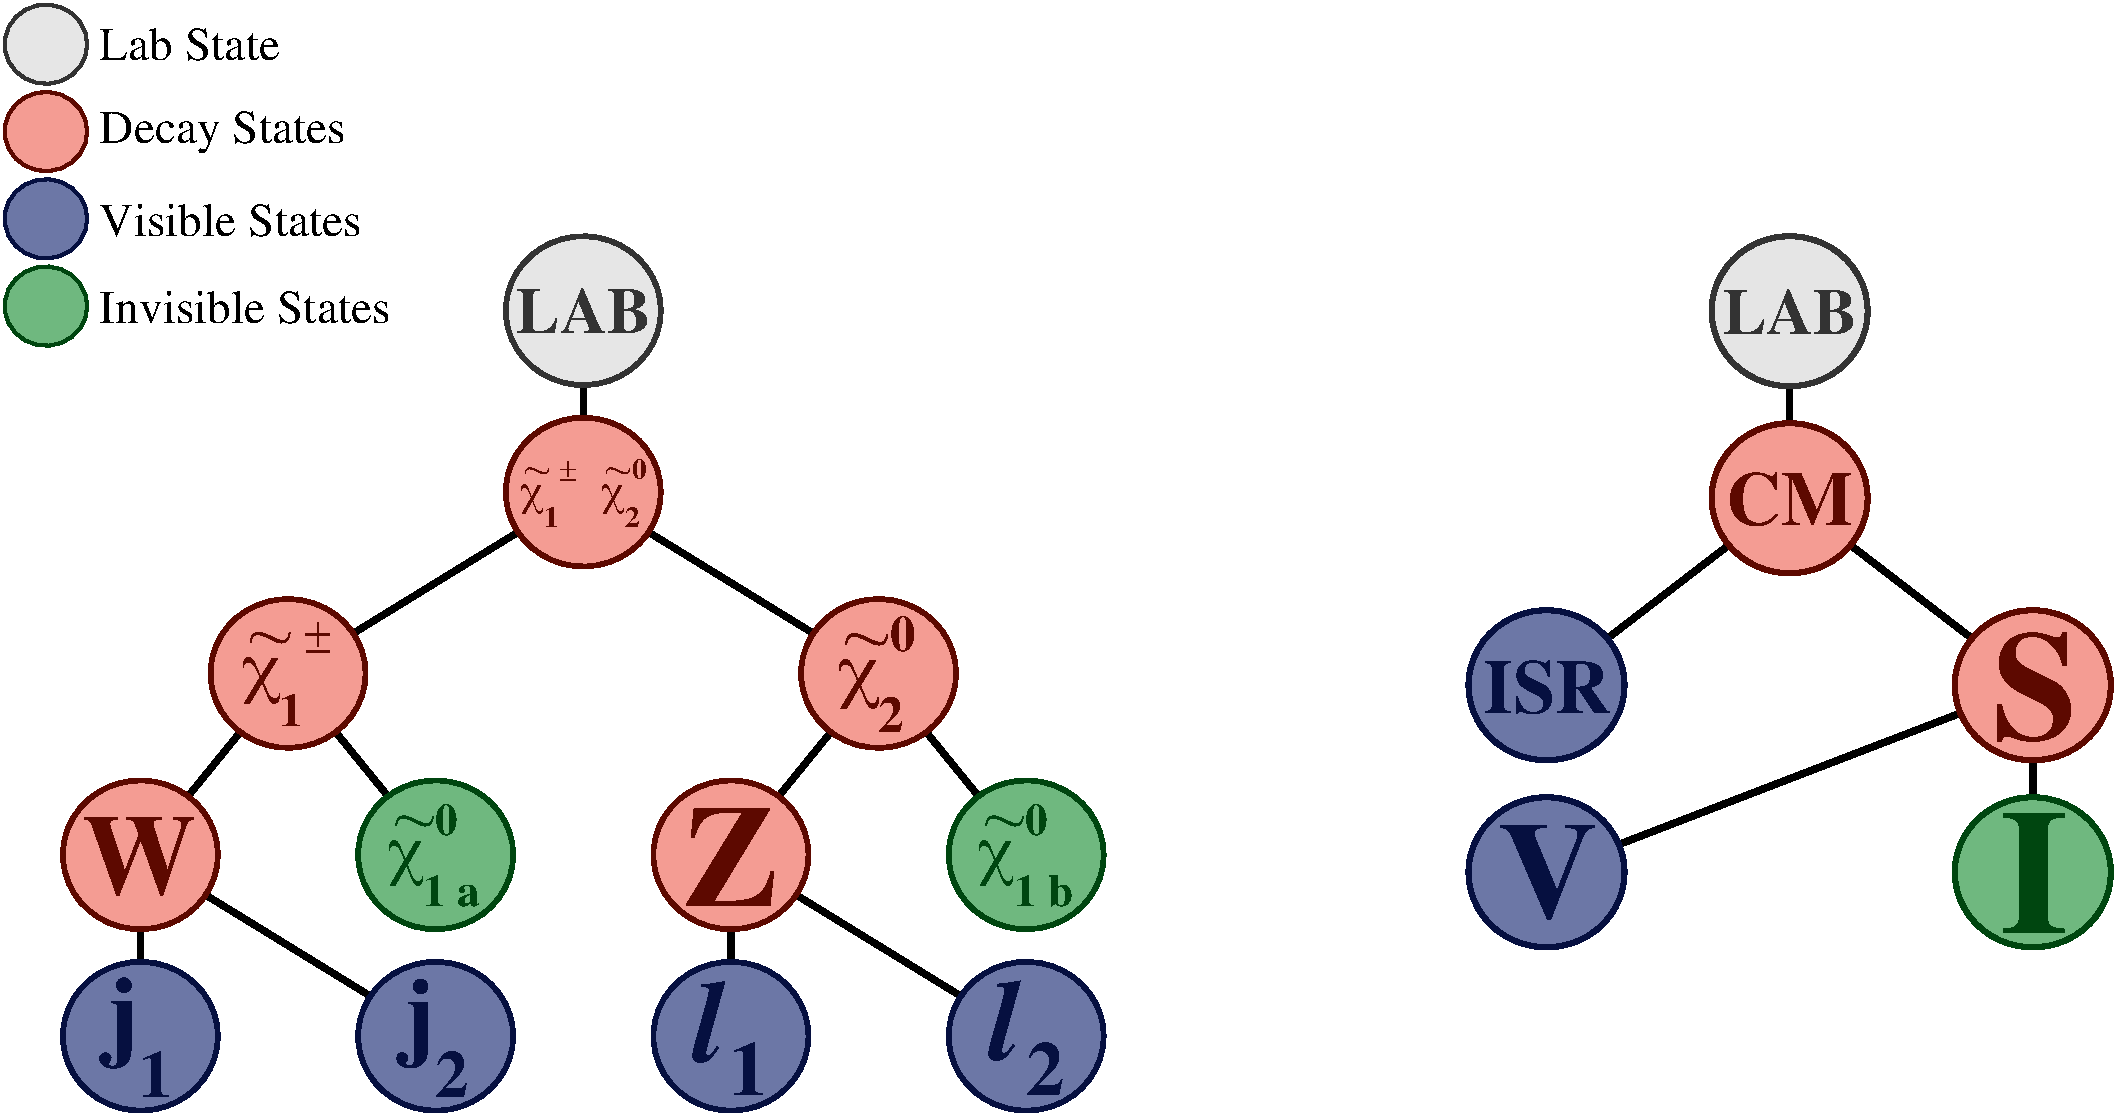
\includegraphics[width=0.9\textwidth]{figures/2ljets_rjr_trees.pdf}
\caption[
Decay trees for the $\twoljets$-RJR analysis
]{%
Decay trees for the $\twoljets$-RJR analysis.
\emph{This figure was made by the RJR team.}~\cite{atlas2022searches}.
Both diagrams represent processes which are targetted in the electroweak
analysis.
(left) A fully-resolved decay tree with its particles labelled.
(right) Only the $Z\rightarrow\ell\ell$ \underline{V}ector boson)
is resolved, but the supersymmetric system recoils off
hard QCD jets labelled ``ISR'', boosting the \underline{I}nvisible particles,
to generate visibly large $\met$ in models with small mass-splittings.
The same approach is used for SR-OffShell selections in the electroweak
analysis.
}
\label{fig:2ljets_rjr_decay_trees}
\end{figure}

The Recursive Jigsaw Reconstruction (RJR) method interprets reconstructed
particle data by reconciling them with user-specified decay trees, and works
by making decisions of how to assign four-momenta to different `systems',
which are nodes of the chosen the decay graph.
Event variables are then evaluated in those systems' rest
frames~\cite{jackson2017sparticles, jackson2017rjr}.

In this way, RJR variables get some intelligence in how parent particles are
reconstructed from their visible decay products, as well as approximate
independence from uninteresting boosts, particularly those from the emission of
QCD jets outside the supersymmetric decay tree.

Over the last several years, RJR event variables have been demonstrated to be
effective for interpreting supersymmetric particle physics
data~\cite{santoni2018probing},
and have been used in numerous \atlas\ searches~\cite{%
atlas_rjr_SUSY_2016_07,
atlas_rjr_SUSY_2016_15,
atlas_rjr_SUSY_2016_16,
atlas_rjr_23l_SUSY_2017_03,
atlas_rjr_SUSY_2018_12,
atlas_rjr_EXOT_2019_19,
atlas_rjr_3l_SUSY_2019_09
}.
They have also influenced the designs of other analyses which do not use
RJR variables themselves~\cite{atlas_rjr_mimic_SUSY_2018_06}.

Two decay trees are used in the $\twoljets$-RJR analysis, with signal region
each.
These trees target C1N2-like scenarios similar to those also considered in the
$\twoljets$-electroweak search,
and illustrated in Figure~\ref{fig:2ljets_rjr_decay_trees}.

\subsubsection{Former excesses}
Excess data were observed in several signal regions of the partial Run~2
search ``for chargino-neutralino production using recursive
jigsaw reconstruction in final states with two or three charged
leptons''~\cite{atlas_rjr_23l_SUSY_2017_03},
which used $36.1~\mathrm{fb}^{-1}$ of proton-proton collisions at
$\sqrt{s} = 13\,\eV[T]$.
That search reported notable excesses in four signal regions.
Of these, two required two charged leptons
($\mathrm{SR}2\ell\_\mathrm{Low}$ and $\mathrm{SR}2\ell\_\mathrm{ISR}$),
and the other two required three
($\mathrm{SR}3\ell\_\mathrm{Low}$ and $\mathrm{SR}3\ell\_\mathrm{ISR}$).

Although the largest local excess was reported as ``$3.0$ standard deviations'',
which is not particularly large, the pattern of four related regions with
excess data can understandably draw attention.

Both $\mathrm{SR}3\ell\_\mathrm{Low}$ and $\mathrm{SR}3\ell\_\mathrm{ISR}$
have been revisited with the full Run~2 data-set and updated background
modelling;
the update sees ``no significant excesses''~\cite{atlas_rjr_3l_SUSY_2019_09}.
These regions have also been approximated without direct use of RJR event
variables;
those approximations also find data ``in agreement'' with the background
model~\cite{atlas_rjr_mimic_SUSY_2018_06}.

The $\twoljets$-RJR serves to analysis reproduce
$\mathrm{SR}2\ell\_\mathrm{Low}$ and $\mathrm{SR}2\ell\_\mathrm{ISR}$,
with the full Run~2 data-set and updated background modelling,
and asks whether the excesses persist.
They do not.

Summary plots for $\twoljets$-RJR and the former 2 and 3 lepton analysis,
including these signal regions with former excesses,
are displayed in Figure~\ref{fig:2ljets_rjr_summaries}.

\begin{figure}[tp]
\centering
\begin{subfigure}{0.48\textwidth}
\centering
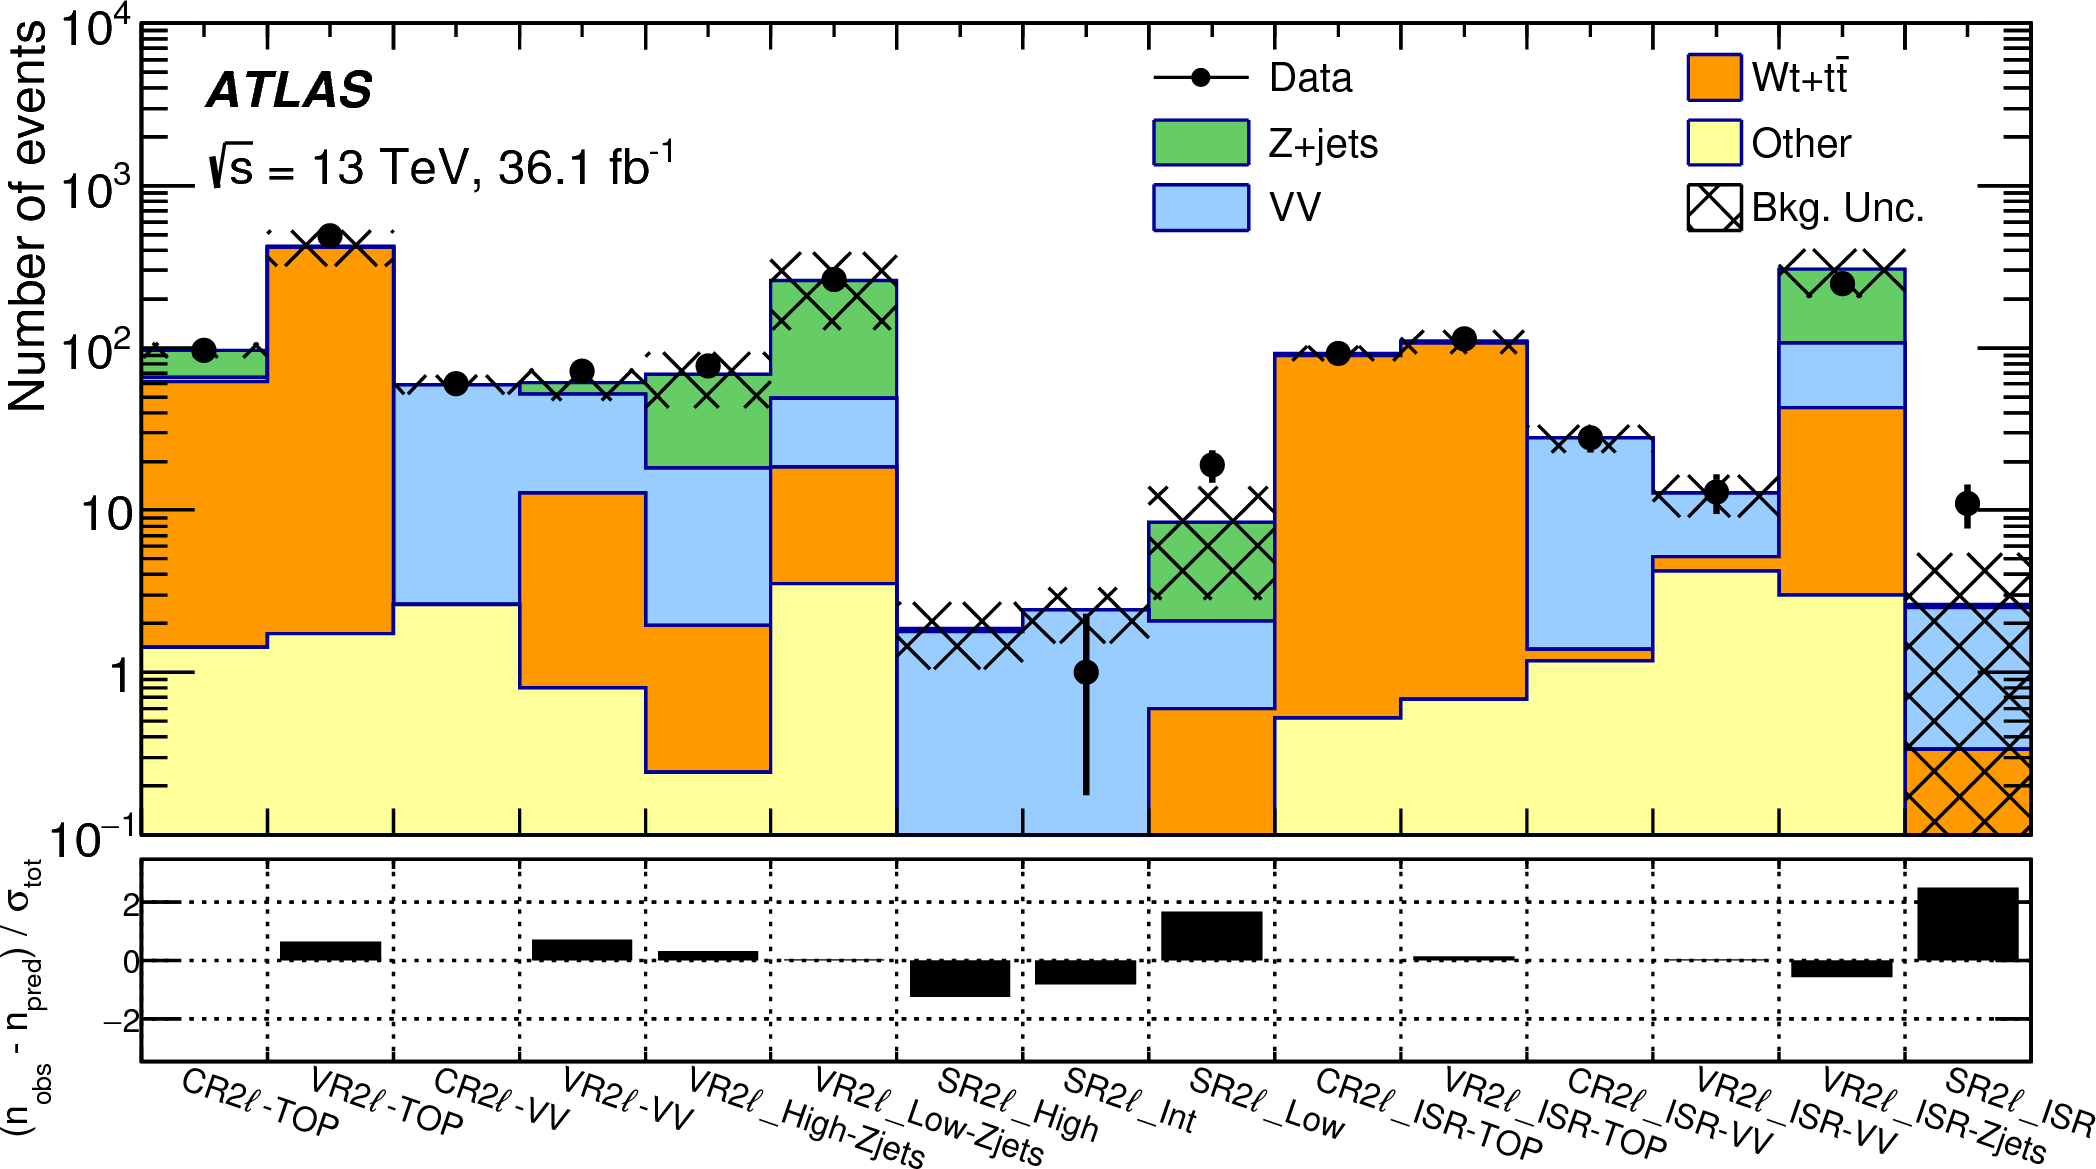
\includegraphics[width=\textwidth]{figures/2ljets_rjr_23l_2l_summary.png}
\caption{$2\ell$ RJR~\cite{atlas_rjr_23l_SUSY_2017_03}}
\end{subfigure}
\hfill
\begin{subfigure}{0.48\textwidth}
\centering
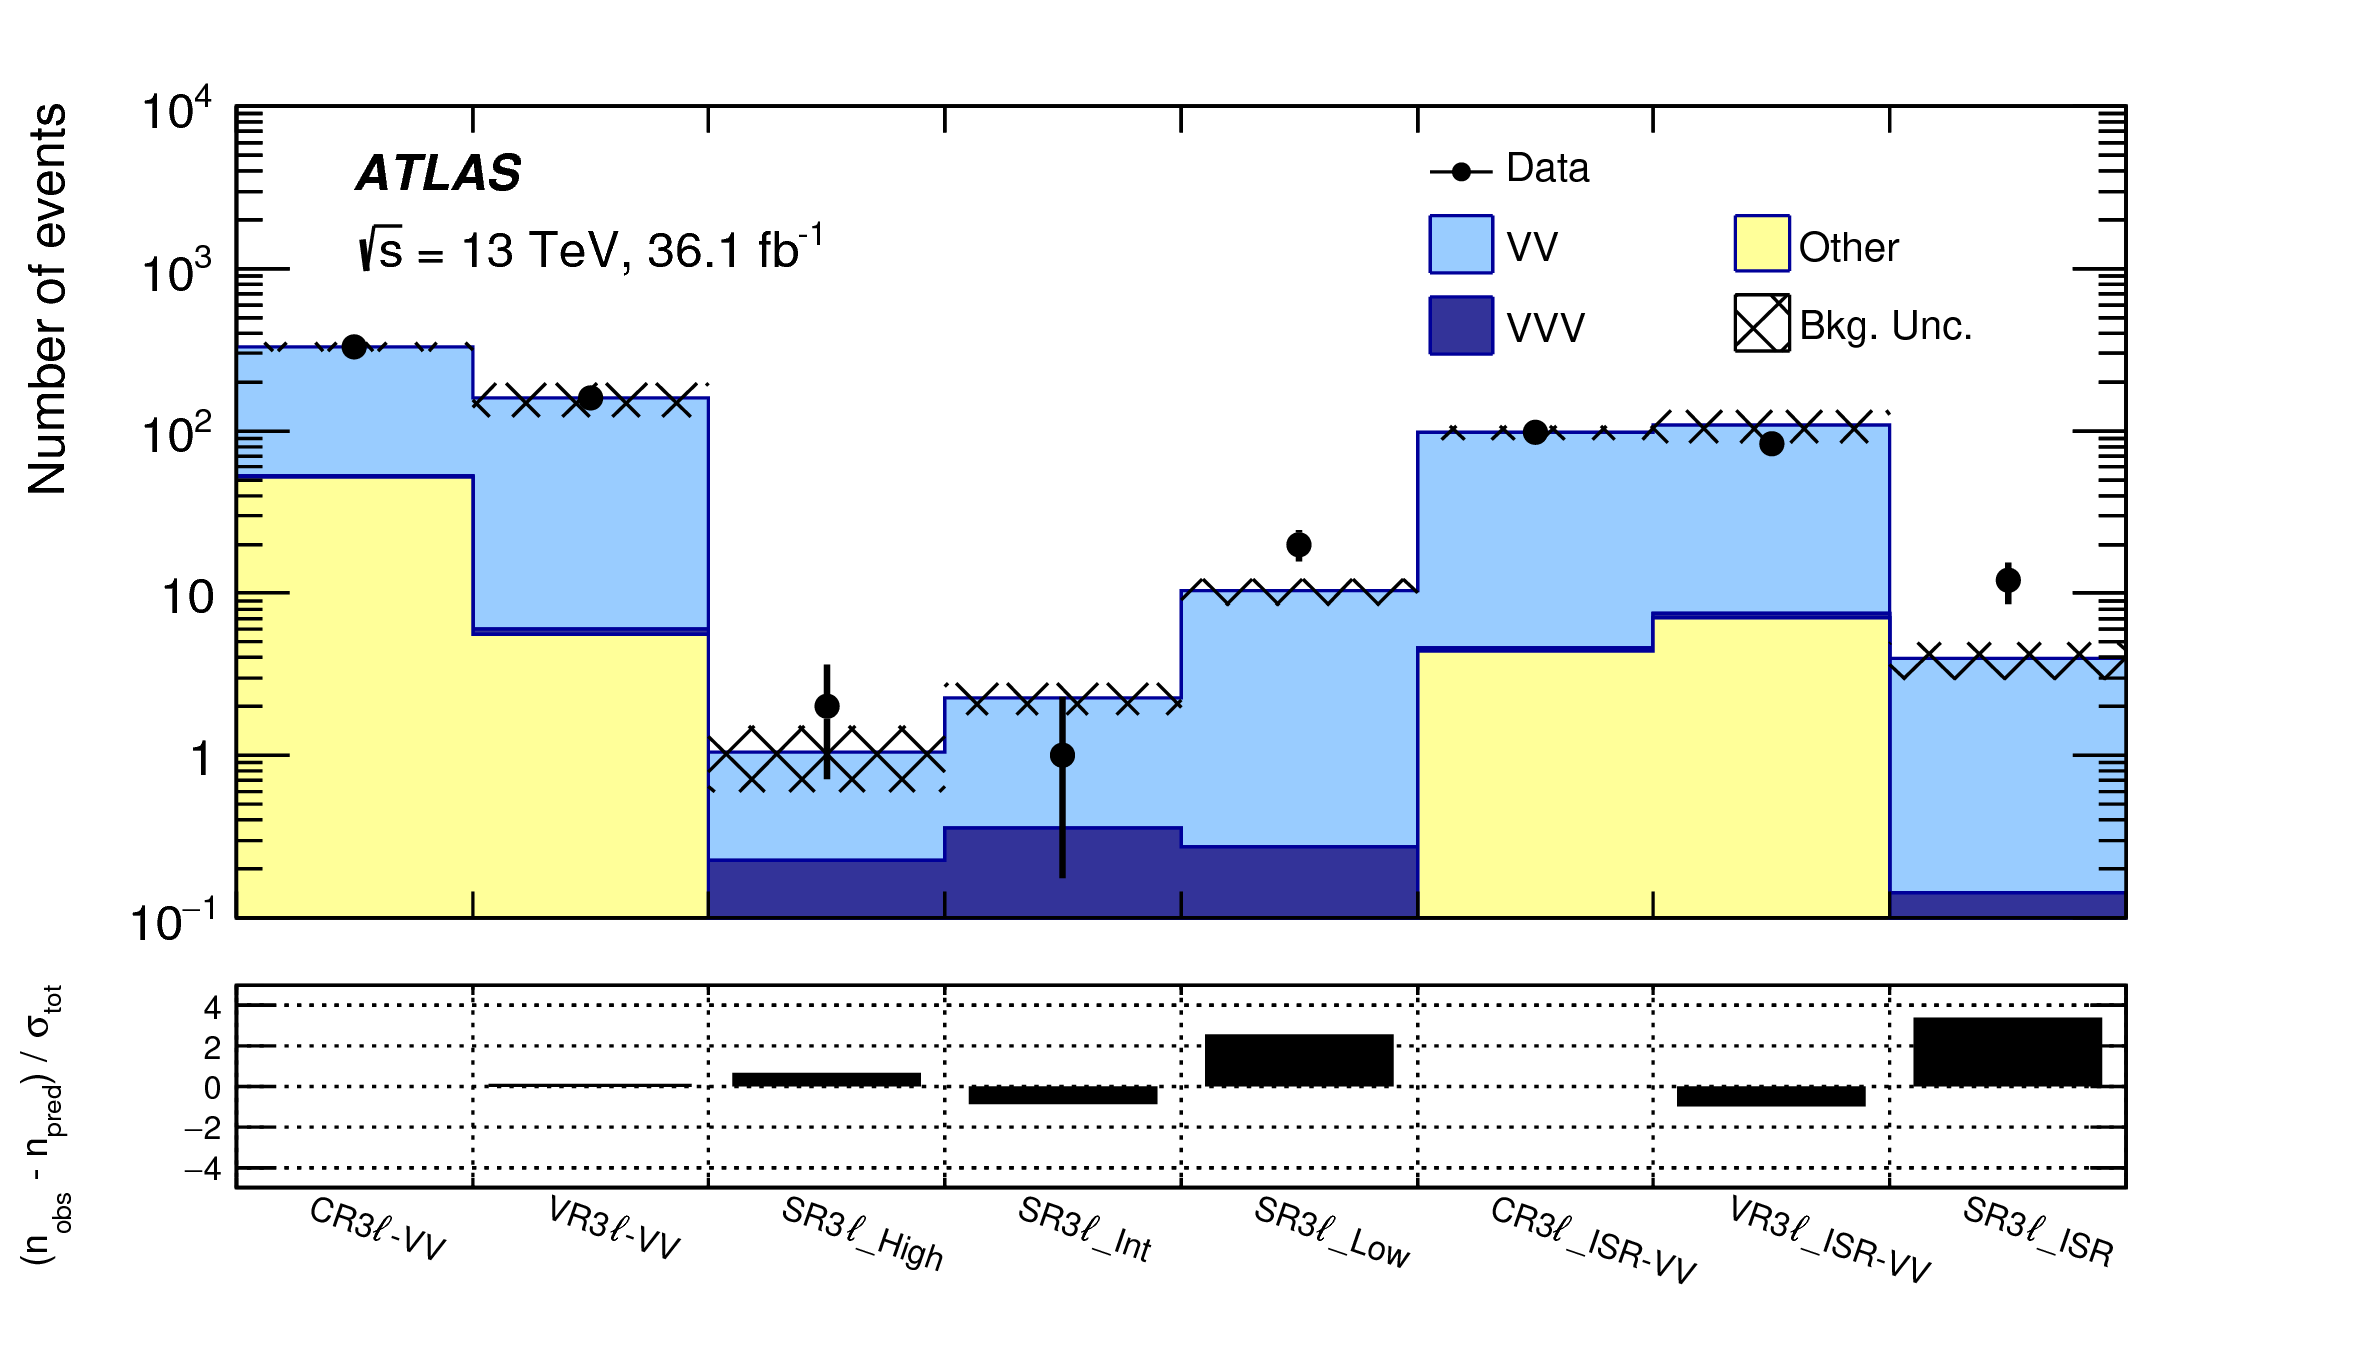
\includegraphics[width=\textwidth]{figures/2ljets_rjr_23l_3l_summary.png}
\caption{$3\ell$ RJR~\cite{atlas_rjr_23l_SUSY_2017_03}}
\end{subfigure}
\\[0.5em]
\begin{subfigure}{0.8\textwidth}
\centering
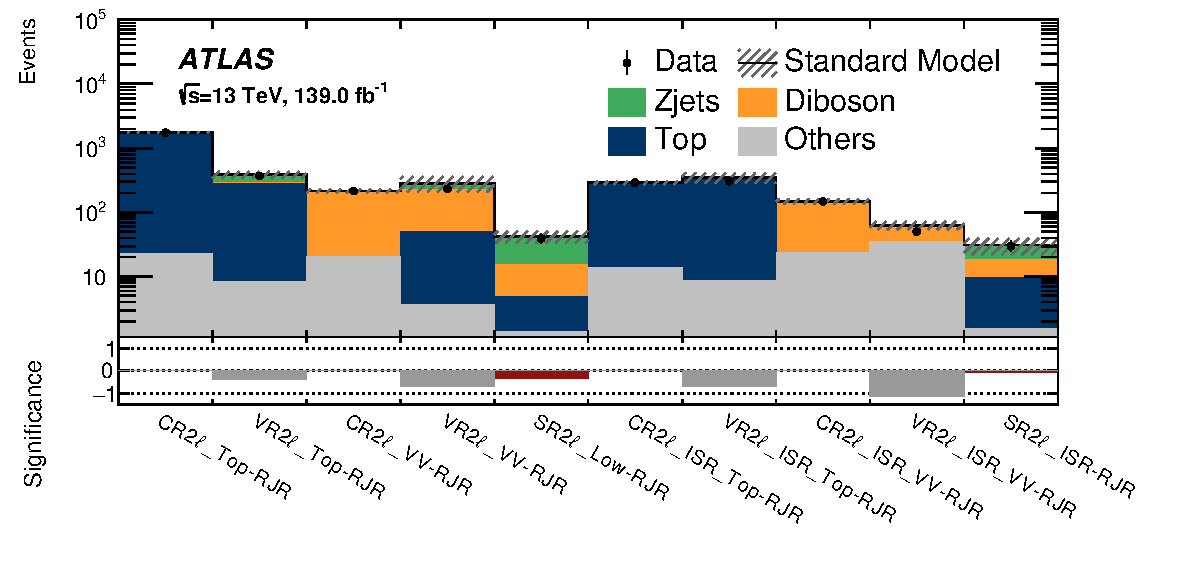
\includegraphics[width=\textwidth]{figures/2ljets_rjr_summary_log.pdf}
\caption{$\twoljets$-RJR~\cite{atlas2022searches}}
\end{subfigure}
\caption[
Summary plots for RJR analyses
]{%
Summary plots for RJR analyses:
(a) and (b)~two- and three- lepton selections respectively,
\emph{reproduced from}~\cite{atlas_rjr_23l_SUSY_2017_03},
(c)~all regions from the $\twoljets$-RJR search~\cite{atlas2022searches}.
Note the excesses in
$\mathrm{SR}2\ell\_\mathrm{Low}$ and $\mathrm{SR}2\ell\_\mathrm{ISR}$ of (a),
and in
$\mathrm{SR}3\ell\_\mathrm{Low}$ and $\mathrm{SR}3\ell\_\mathrm{ISR}$ of (b).
\emph{Sub-figure (c) was made by the RJR team.}
}
\label{fig:2ljets_rjr_summaries}
\end{figure}


\subsubsection{Doubts}
Disappearing excesses have encouraged some doubts about RJR variables in
certain social circles;
the existence of the `RJR-mimic' paper~\cite{atlas_rjr_mimic_SUSY_2018_06}
is public evidence of this.

A more precisely framed problem with RJR variables is that they tend to select
phase space, which is poorly modelled by simulations.
This is plausibly explained by the fact that RJR variables are non-trivially
related to conventional, lab-frame variables.
Simulations have been tuned to model conventional variables well, and
`systematic' variations are evaluated and derived in conventional variables.
Modelling these features accurately does not imply that all other functions of
the data are well understood.
These effects cause Monte Carlo simulations to give predictions in RJR regions
which are inaccurate and/or carry large uncertainties.

A lack of reliable simulations motivates reliance on `data-driven' background
estimates in RJR selections, which, from my perspective, are hard to interpret
or trust.
Indeed, I argue that all `data-driven' methods rely not only on data but on
hypothetical extrapolations which may not be well motivated, particularly when
studying complicated features such as RJR variables.
For these reasons, I choose to not use any RJR event variables in the
$\twoljets$-electroweak analysis.


\FloatBarrier
\subsection{Strong}
\label{sec:2ljets_origins_strong}
Strong supersymmetry, producing super-partners of quarks and gluons, would be
produced at much larger cross-sections than electroweak supersymmetry at the
LHC.
Squarks and gluinos are therefore excluded with masses up to several
$\eV[T]$ using hadronic data alone, depending on which simplified model is
considered~\cite{atlas_susy_strong_0l}.

The $\twoljets$-strong search targets strongly interacting supersymmetric
effects in cases where their decays produce pairs of charged leptons.
Like the RJR and electroweak $\twoljets$ searches, the $\twoljets$-strong
signals produce jets and invisible lightest supersymmetric particles.
Unlike the RJR and electroweak parts, not all of these leptons are produced
by $Z$ boson decays.
As illustrated in Figure~\ref{fig:2ljets_strong_signal_diagrams}, decay trees
featuring sleptons can also produce lepton pairs.
Lepton pairs produced in these slepton interactions are of the same flavour
and opposite charge, like those from $Z$ boson decays, but they have different
mass dilepton mass characteristics.

% signal models
\begin{figure}[tp]
\centering
\begin{subfigure}{0.48\textwidth}
\centering
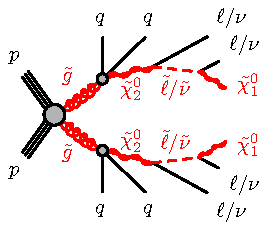
\includegraphics[width=\textwidth]{figures/2ljets_strong_gogo_qqqqllllN1N1_N2.pdf}
\caption{gluino-slepton}
\end{subfigure}
\hfill
\begin{subfigure}{0.47\textwidth}
\centering
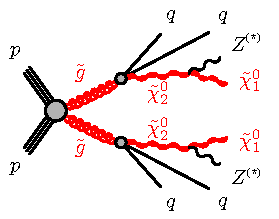
\includegraphics[width=\textwidth]{figures/2ljets_strong_gogo_qqqqZZN1N1.pdf}
\caption{gluino-$Z^{(*)}$}
\end{subfigure}
\\[0.5em]
\begin{subfigure}{0.48\textwidth}
\centering
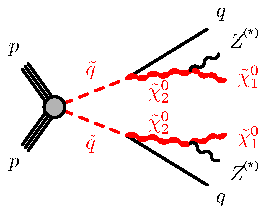
\includegraphics[width=\textwidth]{figures/2ljets_strong_sqsq_qqZZN1N1.pdf}
\caption{squark-$Z^{(*)}$}
\end{subfigure}
\caption[
Supersymmetric signal processes in the $\twoljets$-strong search
]{%
Supersymmetric signal processes in the $\twoljets$-strong search.
\emph{Figures reproduced from the paper%
}~\cite{atlas2022searches, atlas_susy_feynman}.
\\[0.5em]
All models produce same-flavour, opposite-sign lepton pairs along with jets
and $\met$.
The gluino-slepton model (a) has a kinematic endpoint in $\mll$
given in Equation~\ref{eqn:2ljets_strong_max_mll}.
The gluino-$Z^{(*)}$ and squark-$Z^{(*)}$ models decay via $Z$ boson
resonances, which may be forced off-shell for small mass-splittings
$m(\neutralino_2) - m(\neutralino_1) < m(Z)$.
}
\label{fig:2ljets_strong_signal_diagrams}
\end{figure}

Rather than peaking at a resonance mass, these pairs have an $\mll$
distribution with a signature end-point which depends on the masses of other
supersymmetric particles in the
$\neutralino_2 \ldots \slepton \ldots \neutralino_1$
decay chain~\cite{paige1996determining}:
\begin{equation}
\label{eqn:2ljets_strong_max_mll}
\max \mll
= m(\neutralino_2)
\sqrt{1 - \frac{m(\slepton\,)^2}{m(\neutralino_2)^2}}
\sqrt{1 - \frac{m(\neutralino_1)^2}{m(\slepton\,)^2}}
.
\end{equation}

Various previous incarnations of this search have been conducted with similar
selections and target models on in older data, including partial Run~2~\cite{
atlas_susy_strong_2l_partial_run2_1,
atlas_susy_strong_2l_partial_run2,
cms_susy_2016_strong_2l_run2_1,
cms_susy_2016_strong_2l_run2
} and Run~1~\cite{
atlas_susy_strong_2l_run1,
cms_susy_2016_strong_2l_run1
} in \atlas\ and \cms.
From these Run~1 searches, one can cherry-pick excesses
of ``$3.0$ standard deviations'' in \atlas\ \cite{atlas_susy_strong_2l_run1}
and ``$2.6$ standard deviations'' in \cms~\cite{cms_susy_2016_strong_2l_run1}.
These excesses of data above estimated backgrounds were not reproduced in their
early Run~2 updates.

% exclusion plots
\begin{figure}[tp]
\centering
\begin{subfigure}{0.48\textwidth}
\centering
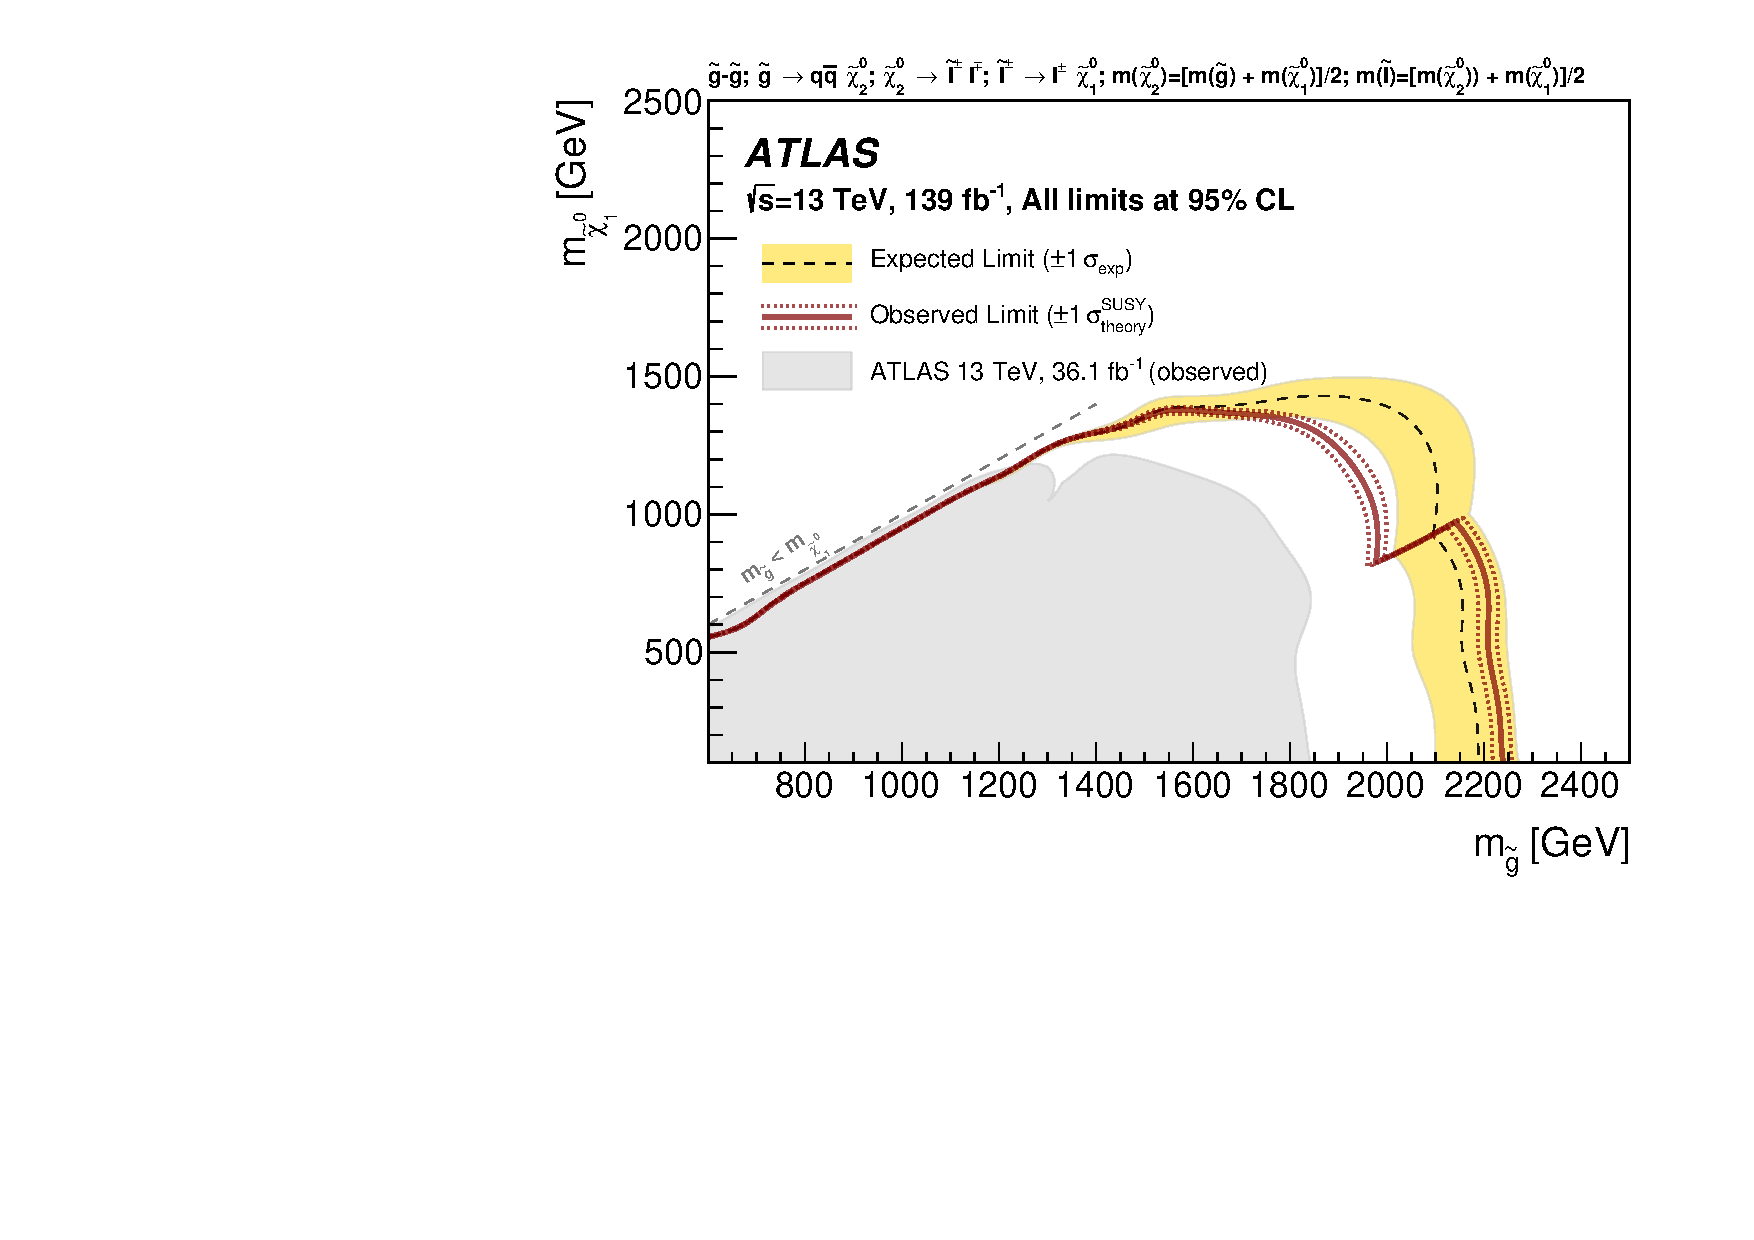
\includegraphics[width=\textwidth]{figures/2ljets_strong_contours_gluino_slepton.pdf}
\caption{gluino-slepton}
\end{subfigure}
\hfill
\begin{subfigure}{0.48\textwidth}
\centering
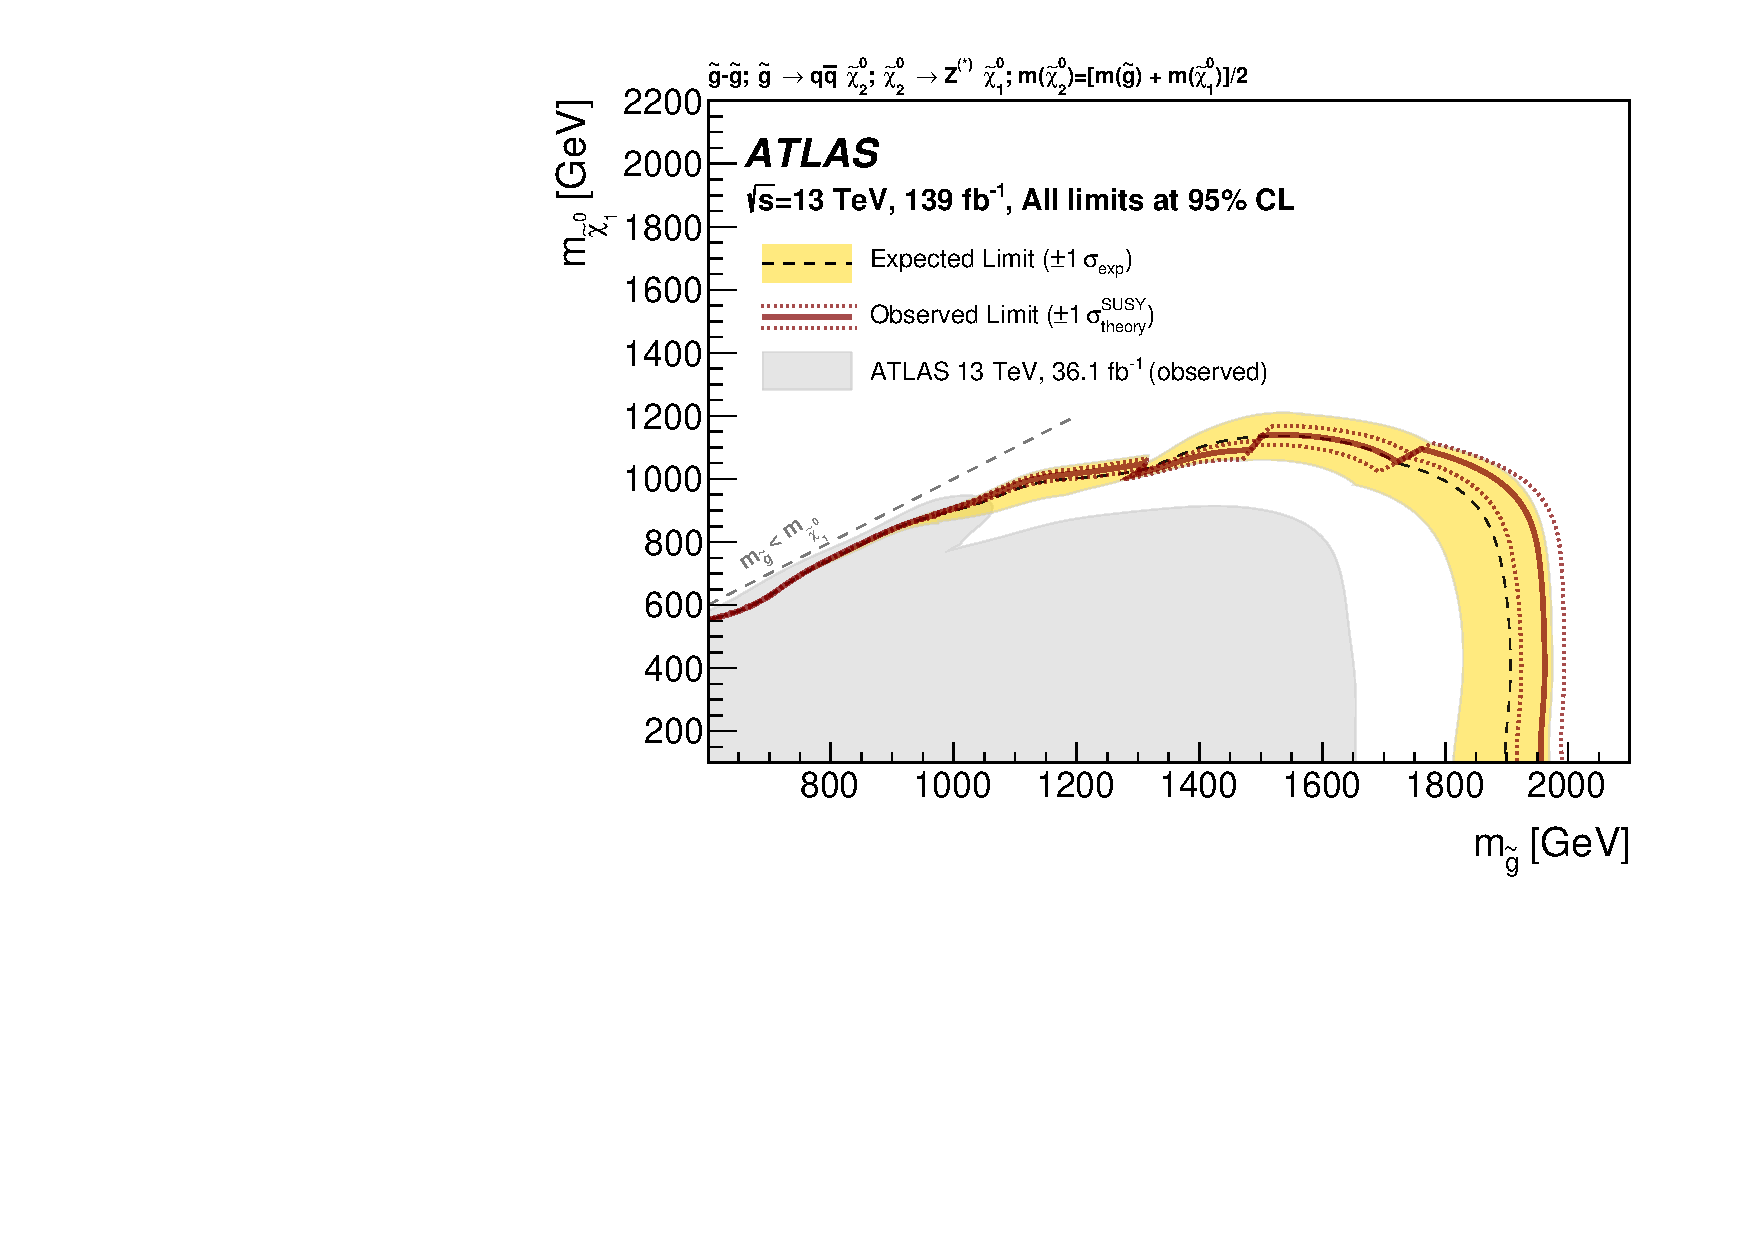
\includegraphics[width=\textwidth]{figures/2ljets_strong_contours_gluino_z.pdf}
\caption{gluino-$Z^{(*)}$}
\end{subfigure}
\\[0.5em]
\begin{subfigure}{0.48\textwidth}
\centering
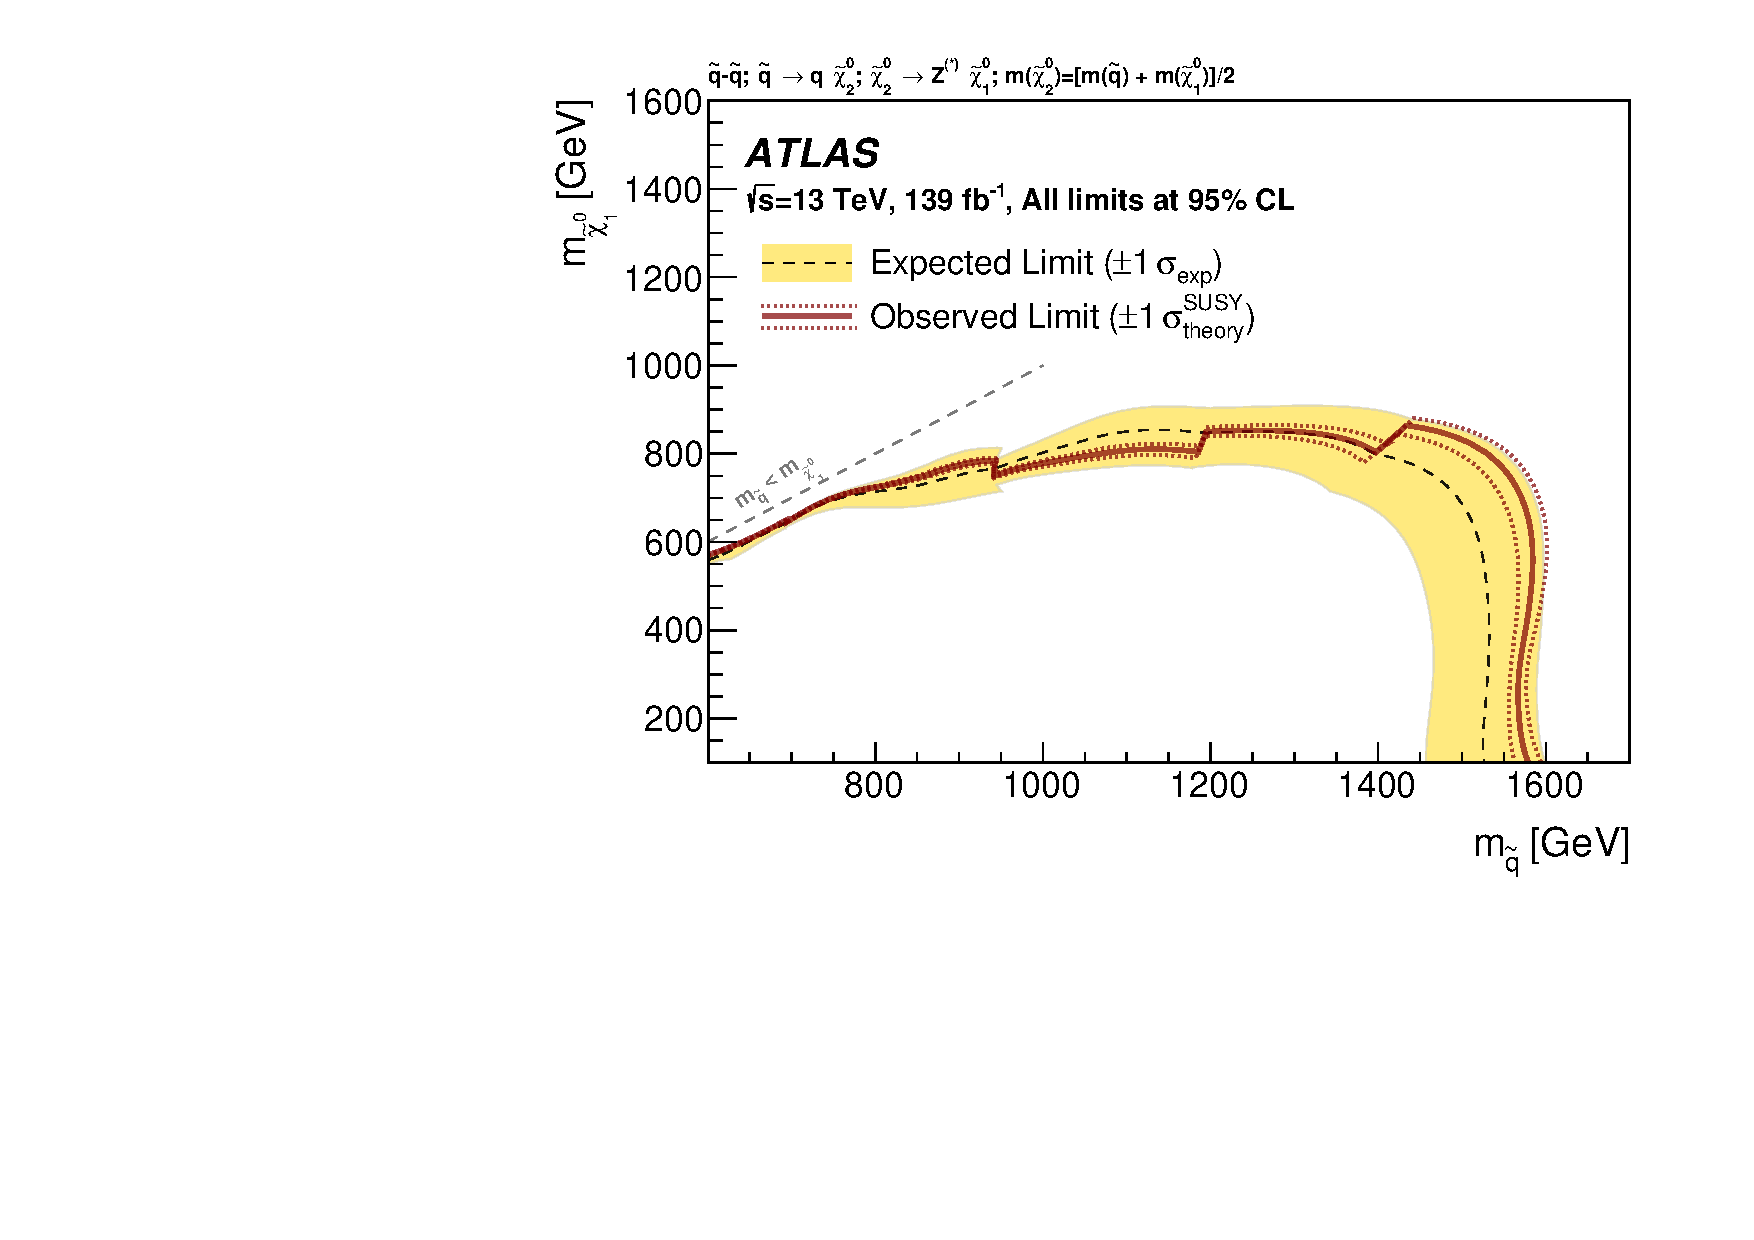
\includegraphics[width=\textwidth]{figures/2ljets_strong_contours_squark_z.pdf}
\caption{squark-$Z^{(*)}$}
\end{subfigure}
\caption[
Contours for signal models of the $\twoljets$-strong search
]{%
Contours for signal models of the $\twoljets$-strong search.
\emph{Figures were produced by the strong team%
}~\cite{atlas2022searches}.
\\[0.5em]
Each model point uses fit results from the signal region with the
``best expected sensitivity'';
jagged edges arise from the switching between contours set by these different
signal regions.
The grey shaded contours showing previous exclusion are taken
from~\cite{atlas_susy_strong_2l_partial_run2}.
}
\label{fig:2ljets_strong_contours}
\end{figure}

To target its signal models, $\twoljets$-strong search defines seven
overlapping signal regions.
Three target on-shell $Z^{(*)}$ models by selecting $\mll$ close to $m(Z)$,
and the others are binned in $\mll$ to give broad sensitivity to the various
kinematic edges across the grid of signal model parameters.

The largest Standard Model background to this search is dileptonic $\ttbar$,
in part because no $b$-jet veto is used.
All three signal models produce same-flavour lepton pairs, but $\ttbar$
produces same-flavour ($ee$/$\mu\mu$) and different-flavour ($e\mu$) pairs at
equal rates.
This difference in flavour symmetry is exploited to estimate backgrounds in
$\twoljets$-strong,
and its previous iterations~\cite{cms_susy_2016_strong_2l_run2_1}.
The estimate works by taking different-flavour data, weighting them by factors
to calibrate for differences in the leptons' reconstruction, and histogramming
them in same-flavour regions.
Simulations for $\ttbar$ and the smaller flavour symmetric backgrounds
$tW$, $WW$, and $\tau\tau$ are replaced by this estimate.

Post-fit results match the data to within $1$-sigma in all $\twoljets$-strong
regions.

Exclusion contours from the $\twoljets$-strong search are reproduced in
Figure~\ref{fig:2ljets_strong_contours}.
Besides their increased reach, the jagged edges to parts of these contour are
striking.
These arise from the combination of results from overlapping signal regions.
Because they overlap, they are not independent and cannot be trivially
combined.
Instead, each model in the signal grid is assigned to the signal region
with the ``best expected sensitivity'' by some measure.
An exclusion contour is constructed for each signal region, then those contours
are joined such that models assigned to each region use its corresponding
contour.

Personally, I find this hard to interpret.
If I had a pet theory which landed near to one of these sharp
region-transition edges, what should I make of these data?
Could some combination of the regions not have combined their information to
produce more precise contours?
Since model predictions change continuously, should our inferences not also?
To aid interpretations and to allow combinations of regions'
information, I chose to design the $\twoljets$-electroweak with only orthogonal
regions, and without any manual switching of regions between models.


\FloatBarrier
\subsection{Electroweak}
\label{sec:2ljets_origins_electroweak}
As motivated in the previous sections, I have personal preferences for
simulation-driven backgrounds and orthogonal multi-bin regions.
This is because simulation-driven estimates are interpretable as
Standard Model predictions,
and orthogonal regions have independent likelihoods which can be cleanly
combined to leverage the information in their data.

The main idea behind the design of the $\twoljets$-electroweak analysis is to
update the regions of the partial Run~2 search in its $\twoljets$
channel~\cite{atlas_23l_SUSY_2016_24}, which also searched for signal models
producing chargino-neutralino pairs which decay via $W$ and $Z$ bosons.
A particular goal was to improve sensitivity by replacing their overlapping
`SR2-int' and `SR2-high' regions with orthogonal selections.
\emph{Special thanks to Sarah~Williams for suggesting this approach.}

As in the $\twoljets$-strong search, the partial Run~2 search chose one
signal region from an expected sensitivity for each signal point,
as displayed in
Figure~\ref{fig:2ljets_23l_stuff}
with the two regions and exclusion contours.

\begin{figure}[tp]
\centering
\begin{subfigure}{0.6\textwidth}
\centering
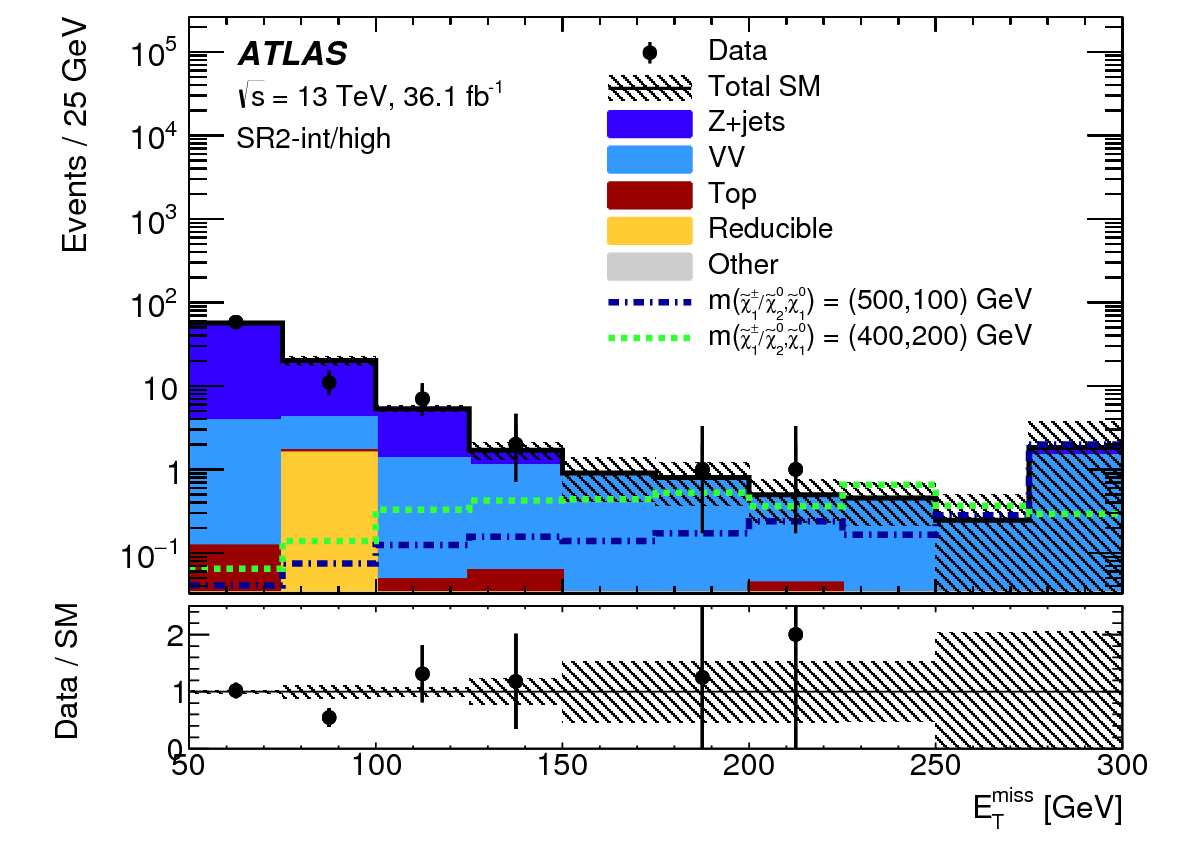
\includegraphics[width=\textwidth]{figures/2ljets_23l_sr2inthigh.png}
\caption{SR2-int and SR2-high}
\end{subfigure}
\\[0.5em]
\begin{subfigure}{0.52\textwidth}
\centering
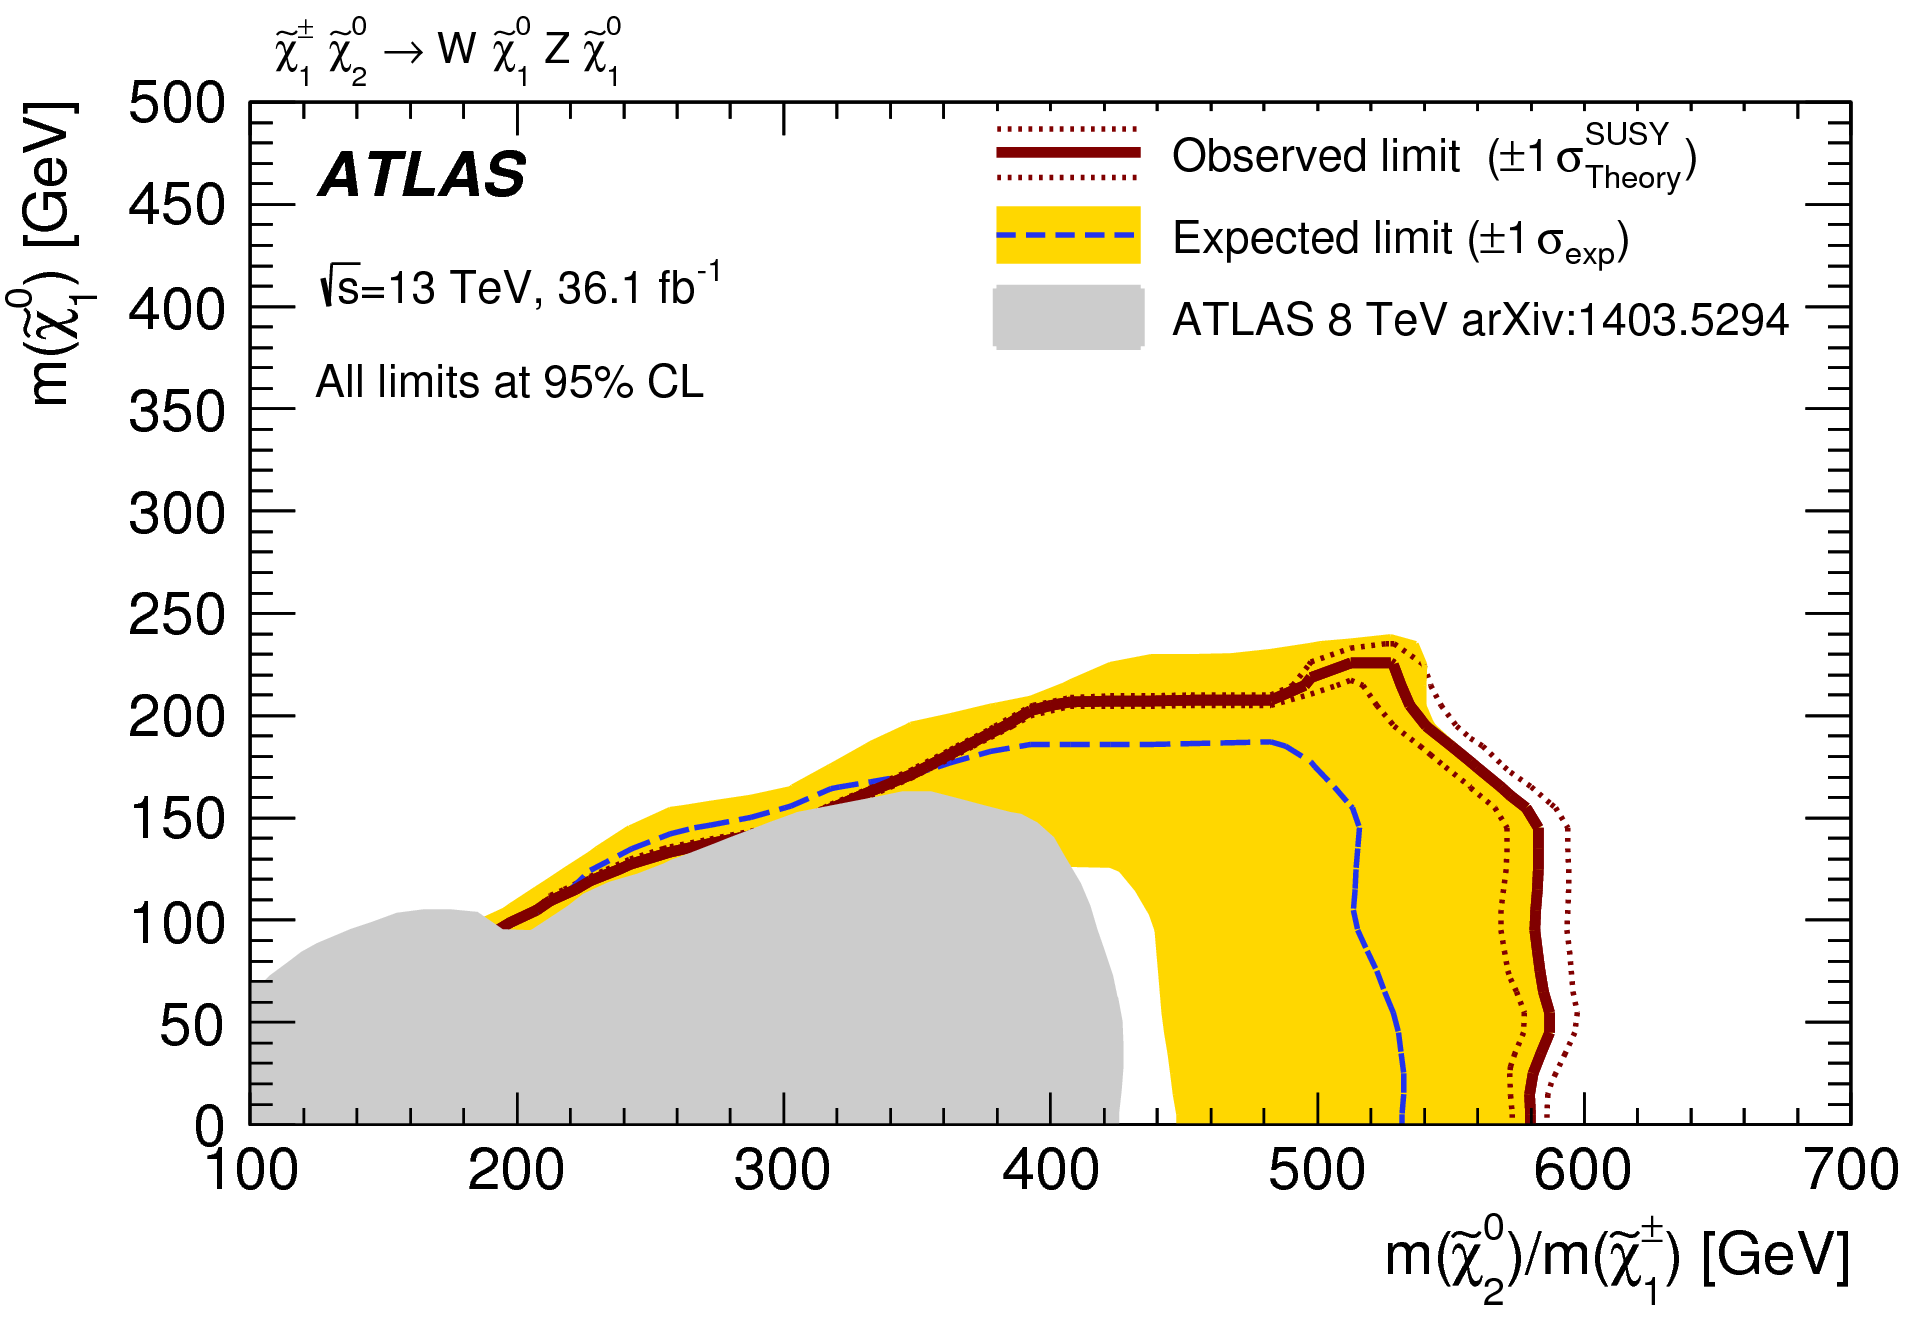
\includegraphics[width=\textwidth]{figures/2ljets_23l_contours_fig_08d.png}
\caption{Combined exclusion}
\end{subfigure}
% \hfill
\begin{subfigure}{0.46\textwidth}
\centering
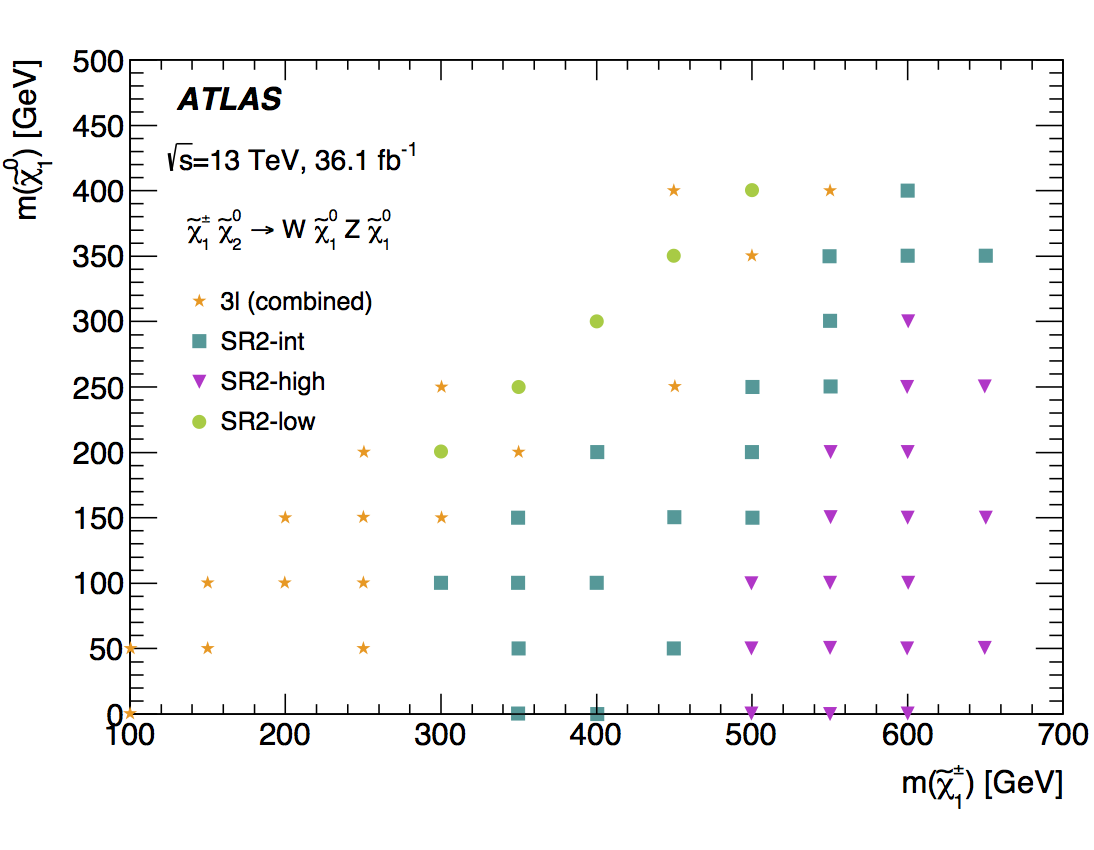
\includegraphics[width=\textwidth]{figures/2ljets_23l_chosen_regions.png}
\caption{Chosen regions}
\end{subfigure}
\caption[
Figures reproduced from the partial Run~2 search with $2/3\ell$ selections
]{%
Figures reproduced from the partial Run~2 search with $2/3\ell$
selections~\cite{atlas_23l_SUSY_2016_24, hepdata.81996}.
\\[0.5em]
(a) Histogrammed distribution of $\met$ in and below SR2-int and SR2-high with
example signal models.
SR2-int requires $\met > 150\,\eV[G]$ and SR2-high requires $\met > 250\,\eV[G]$.
\\[0.5em]
(b) Contours for the combined $\twoljets$ and $3\ell$ channels.
Each signal point chooses a signal region, which is displayed in (c).
The grey region shows exclusion from a previous search in Run~1
data~\cite{atlas_2l_SUSY_2013_11}.
\\[0.5em]
(c) Signal regions selected for each signal point in the grid.
Two-lepton selections occupy the largest mass-splittings.
The $3\ell$ regions are orthogonal and combined.
}
\label{fig:2ljets_23l_stuff}
\end{figure}

Additionally, $\twoljets$ widens its scope to target a GMSB simplified model
illustrated in Figure~\ref{fig:2ljets_signal_diagrams}.
The C1N2 and GMSB models behave similarly since both feature decays via massive
bosons ($W\kern-0.4exZ$, $ZZ$ or $Zh$) to leptons and jets, in similarly structures decay
trees to pairs of invisible supersymmetric particles.
Although widening sensitivity to both models does sacrifice sensitivity to
either one, the increased degree of model independence is itself of value for
future reinterpretations of the data.
We are happy to sacrifice some precision for generality.

Multi-bin fits are not special.
They are standard \atlas\ practice, and there could have been no complication
in replacing the overlapping SR2-int and SR2-high with orthogonally binned
regions.
However, my design decisions for $\twoljets$-electroweak
caused problems for the clarity of communication and accuracy of background
modelling.
These issues are developed further through the remainder of this chapter.

A multi-binned histogram is usually and clearly illustrated as slicing up one
variable.
My design of $\twoljets$-electroweak violates this.
Instead, it is designed as a tree whose branches recursively split various
variables.
This leads to specifications which are challenging to present and understand,
and which require region names with numerous suffixes to specify where they
live in that tree.

Worse, I disregarded the idea that every region should have a large
background expectation.
Normally, this is justified by the limitations of approximate statistical
methods, which work
``from as few as $\mathcal{O}(10)$ data events''~\cite{histfitter2014}.
But the Poisson likelihood works for infinitesimally small
expectations~\cite{skilling2009cosmology}, and in the small-bin limit one has
continuous distributions with Poisson normalizations
(sometimes called ``extended'' in high-energy
physics~\cite{barlow1990extended})
that are standard and easily analysed.

Events appearing in a region with minimal background is evidence in favour
of new contributions, and that only strengthens as the background approaches
zero.
For example, the top quark was observed by \dzero\ using seven regions all with
background expectations of $1$ or less, for a total of $3.79\pm0.55$ expected
and $17$ observed~\cite{abachi1995observation}.
If they could do that with technology from the year $1995$, we can do it now.

The real reason to avoid small backgrounds is, in this context, to allow honest
assignments of background uncertainties.
Although main simulated samples may have good precision,
many `systematic' variations and `data-driven' estimates are also required.
Many of these alternative estimates have far worse precision, and can fail
totally as the number of simulated events accepted plunges towards zero;
they can require $\approx10$ data events to work properly.

Unfortunately, $\twoljets$-electroweak selections were finalized before I
appreciated this problem that background variations were dubious.
Various workaround are invoked to assign plausible variations despite small
yields, which we shall in the remainder of this chapter.

As seen in the splash summary of Section~\ref{sec:2ljets_splash}, this search
finds agreement with backgrounds except for some local deficits of data below
backgrounds.
Exclusion contours exceed their expected range because of these deficits,
but they can only be trusted if the background model is trusted.

Searches have been performed in \cms\ for similar
C1N2~\cite{cms_susy_2022_c1n2} and GMSB models~\cite{
cms_susy_2018_partial_run2_combination,
cms_susy_2022_gmsb
}, with comparable results.

\TODO{other atlas C1N2 and GMSB searches (combinations, 3L offshell exclusion)}


\section{Events}
\label{sec:2ljets_events}
\TODO{make sure we say 136ifb from 2015 to 2018 run 2 data. Good run lists etc}

This section describes the events selected for the $\twoljets$ searches, the
reconstructed particle objects derived from those events and various
important event variables.

From its name, it is clear that $\twoljets$ analyses features of events with
two charged leptons (electrons or muons --- not taus), and at least one jet.
Though not nominal, a $\met$ requirement is also implicit from the context
of $R$-parity conserving supersymmetric models.
This section serves to describe how events are selected for the $\twoljets$
analyses, and which event variables are extracted for use in its selections.

Triggers and object definitions are shared between the three $\twoljets$
searches.
Higher level event variables and selections will only be described for the
$\twoljets$-electroweak search.

\subsection{Trigger}
\label{sec:2ljets_trigger}
There would be no event variables if not for the trigger.
When living our daily lives, we are bombarded with sensory data and must pay
attention only those gems few of any use, to avoid exhausting our
processing capacity.
Running \atlas\ is no different.

Each trigger in \atlas' arsenal activates on a selection comprising some
combination of sufficiently hard objects.
The set of targeted objects includes all those used in this analysis and more:
electron, muons, jets, $b$-jets, $\met$, as well as photons and hadronically
decaying tau leptons~\cite{atlas_PERF_2007_01}.

The list of available triggers in \atlas\ is designed to balance data rates
against physical interest.
It includes a variety of general purpose selections, which are used for
$\twoljets$, along with more specialized targets such as vector boson fusion
or long-lived particles.
The list varies through time, so we select triggers specifically in
each data-taking period.

The loosest triggers are `prescaled' --- their data rate is reduced by randomly
accepting only a small fraction of events.
Prescaling adds complication which we avoid;
for $\twoljets$, we use only the `lowest' (loosest, highest rate) un-prescaled
triggers selecting two charged leptons~\cite{atlas_twiki_lowest_unprescaled}.
Those charged leptons are selected in the
high-level trigger (described in Section~\ref{sec:atlas_trigger})
primarily requiring large $\pt$ and certain quality criteria which vary by
trigger.

In total, we use $14$ different two-lepton trigger selections, each of which
selects for an electron pair, a muon pair, or an emu (electron-muon pair).
To describe those triggers, let $\pt^{\ell_i}$ be the transverse momentum of the
$i\mathrm{th}$ hardest lepton.

In short, all triggers require $\pt^{\ell_i}$ values to exceed thresholds in
the range $8\textrm{--}26\,\eV[G]$.
To detail all trigger requirements and their variations with data period
would be too tedious and not enlightening, but their $\pt^{\ell_i}$ requirements
are summarized here.
Please do not read them all in detail.
\begin{itemize}
\item Electron pair: requirements vary between
\begin{itemize}
\item $\pt^{e_2} > 12\,\eV[G]$ and
\item $\pt^{e_2} > 17\,\eV[G]$.
\end{itemize}
\item Muon pair: various requirements include
\begin{itemize}
\item $\pt^{\mu_2} > 10\,\eV[G]$,
\item $\pt^{\mu_2} > 14\,\eV[G]$,
\item $\pt^{\mu_1} > 18\,\eV[G]~\&~\pt^{\mu_2} > 8\,\eV[G]$, and
\item $\pt^{\mu_1} > 22\,\eV[G]~\&~\pt^{\mu_2} > 8\,\eV[G]$.
\end{itemize}
\item Emu pair: various asymmetric requirements include
\begin{itemize}
\item $\pt^{e_1} > 17\,\eV[G]~\&~\pt^{\mu_1} > 14\,\eV[G]$,
\item $\pt^{e_1} > 7\,\eV[G]~\&~\pt^{\mu_1} > 24\,\eV[G]$, and
\item $\pt^{e_1} > 26\,\eV[G]~\&~\pt^{\mu_1} > 8\,\eV[G]$.
\end{itemize}
\end{itemize}
The point of listing these is to demonstrate trigger activations are
non-trivial.
This motivates lepton selections which exceed these trigger thresholds,
to avoid the need to model their jagged activations and variable
efficiencies near to those thresholds~\cite{
atlas_trigger_egamma_run2,
atlas_trigger_muon_run2
}.
Throughout the data used in $\twoljets$, trigger requirements
have increased in hardness with time.


\subsubsection{Alternative triggers}
Why should we only use two-lepton triggers?
Alternatives could be one-lepton triggers, for cases where the other is not
reconstructed at trigger level, or perhaps also triggers for jets and $\met$.
The answer is that the benefits of additional triggers were assessed to not
outweigh the cost of using them.

The benefit of an additional trigger could be in increased signal yields if
that trigger does not also harmfully increase inseparable backgrounds.
A study, \emph{which was performed by Knut Vadla}, investigated the effects
of including one-lepton triggers.
In a signal-region-like selection requiring two leptons, two jets and
$\met > 200\,\eV[G]$, this study showed that two-lepton triggers already accept
in excess of $90\%$ of events from benchmark C1N2 models.
Therefore, any additional trigger has at most a $\approx10\%$;
improvement. Adding one-lepton triggers was found to increase efficiency by
only a few percentage points, depending on the model.
We considered that to be too little to be worthwhile.

Costs of triggers are attributable to human effort;
software work to include them and their associated Monte Carlo weights, along
with studies to validate background estimates and evaluate systematic
uncertainties.
Similarly, our implementation of the Matrix Method fake/non-prompt lepton
background estimate (see Section~\ref{sec:2ljets_mm_fakes}) is not equipped to
handle one-lepton triggers.

Although jet and $\met$ triggers were not studied in detail, they can be
quickly ruled out since they hard objects: examples of these triggers require
approximately $\ptjone > 400\,\eV[G]$, $p_\mathrm{T}^{\,j_3} > 200\,\eV[G]$, or
$\met > 100\,\eV[G]$~\cite{atlas_twiki_lowest_unprescaled}.
Leptons, however, are striking signals which are produced as smaller background
rates, as they suppressed by electroweak couplings.
Therefore, \atlas\ can trigger on leptons with much softer requirements;
lepton triggers allow us to use softer jets and $\met$, which are relied upon
throughout the $\twoljets$ analyses.


\subsection{Leptons}
\label{sec:2ljets_events_leptons}
In the context of $\twoljets$, `leptons' means `electron-or-muons';
this is because taus, which decay before reconstruction, and are not used
directly in $\twoljets$, and neutral leptons (the neutrinos) go missing.

Reconstructed lepton objects feature momenta, charges, and flavours.
Each is included only if it satisfies certain kinematic and
is identified with `quality' criteria.
For both electron and muons, these criteria are standardized with labels
`loose', `medium', and `tight'.
These are nested, in the sense that tight implies medium,
and medium implies loose.
Other, more specialized, criteria exist, but they are not relevant $\twoljets$.

Muons are identified by fitting tracks to hits in the inner tracker and muon
spectrometer.
Their quality criteria use goodness-of-fit metrics from those fits, along with
low-level details of detector interactions.
Tighter requirements primarily act to reduce from non-prompt backgrounds,
which are muons from hadronic decays~\cite{atlas_muon_quality_MUON_2018_03}.

Electron identification combines data from the inner tracker and
calorimeters.
Electron quality criteria use numerous features of detector
interactions, track fitting metrics, the matching of tracks to calorimeter
clusters, calorimeter shower shapes, and leakage into the hadronic calorimeter.
Tighter requirements reduce backgrounds, which include misidentified objects
--- photons and hadrons --- as well as non-prompt electrons from hadronic
decays~\cite{atlas_egamma_quality_EGAM_2018_01}.

Isolation of leptons from nearby hadronic activity is another feature which
can be used to reduce misidentification rates.
Standard isolation definitions exist for both electrons and muons in a similar
structure to the quality criteria.

Leptons in $\twoljets$ are further sliced into two classes:
`baseline' and `signal'.
Baseline leptons and are used in background estimation methods and to ensure
orthogonality with other \atlas\ analyses, which study events with differing
lepton counts.
Baseline requirements are softer and lower quality than signal requirements.

Any event used in regions of the $\twoljets$-electroweak analysis is required
to have exactly two baseline leptons and exactly two signal leptons, meaning
that the event has two reconstructed leptons which pass both sets of criteria.
This vetoes events with soft or low quality third leptons, ensuring that those
three-lepton events can be used independently in other studies.

Baseline leptons are required only to have $\pt > 3\,\eV[G]$ for muons and
$\pt > 4.5\,\eV[G]$ for electrons.
Signal leptons are all required to have $\pt > 10\,\eV[G]$, along with tighter
quality and isolation requirements, details of which are given in the
paper~\cite{atlas2022searches}.
Electrons are accepted within $|\eta| < 2.47$.
Baseline muons have $|\eta| < 2.7$, and signal muons have $|\eta| < 2.6$.


All leptons used in regions of the $\twoljets$-electroweak analysis are signal
leptons with $\pt > 25\,\eV[G]$.
This harder requirement reduces backgrounds, moves our selections away from the
lowest trigger thresholds, and matches the precedent set by previous
work~\cite{atlas_23l_SUSY_2016_24}.


\subsection{Jets}
Like leptons, hadronic jets are identified with `baseline' and `signal'
requirements, with increasingly tight requirements on quality metrics and
kinematics.

Jets in $\twoljets$ use the anti-$k_t$ algorithm with the standard small-radius
parameter of $R=0.4$~\cite{jet_anti_kt}.
Jets are formed from `topological' clusters of energy deposits in the
calorimeters~\cite{atlas_jet_topo_PERF_2014_07}.

This topological clustering algorithm is no longer the \atlas-recommended jet
algorithm; it has been supplanted in recent years by a `particle flow' method,
which uses tracking information to improve the reconstruction of charged
hadrons~\cite{atlas_jet_pflow_PERF_2015_09}.
We did not attempt to switch to these improved jets because the change in
policy occurred during the years this analysis was in development, and the
change would have required more work and even more delays.

Baseline jets are defined to require $\pt > 20\,\eV[G]$ with $|\eta| < 2.8$;
signal jets additionally require $\pt > 30\,\eV[G]$.
To reduce the impact of pile-up jets, a variety of quality criteria are used,
depending on the jet $\pt$ and $|\eta|$.
Details of these quality criteria and angular selections are given in the
paper~\cite{atlas2022searches}.


\subsection{\textit{b}-jets}
\label{sec:2ljets_btagging}
Tagging adds labels to objects.
Unlike how electrons and muons are very cleanly separated, however, jet tagging
is a more noisy affair.
Taggers are available for various jet properties, such charm flavour ($c$-jet),
bottom flavour ($b$-jet).
Of these, $\twoljets$ uses only $b$-tagging.

Larger radius jets can also use taggers for heavy decays, such as those from
$W$, Higgs or top resonance, but large radius were considered too much
additional work to considered in $\twoljets$.

Jets originating from $b$ quarks are distinct due to the long lifetimes and
long decay trees of $B$-hadrons, both of which leave signals in \atlas'
inner trackers.

For jets in $\twoljets$, $b$-tagging is useful to separate events due to
$\ttbar$ backgrounds (since their weak decays almost always produce $b$
quarks), and to select for signals producing $Z/h \rightarrow b\bar b$ decays
in the GMSB model.

Signal $b$-jets in $\twoljets$ require $\pt > 20\,\eV[G]$, $|\eta| < 2.5$ and a
tag from the `MV2c10' boosted decision tree
algorithm~\cite{
friedman2002stochastic,
atlas_jet_mv2c10_2017,
atlas_jet_tagging_2019
} at its $77\%$ efficiency working point.
This efficiency means that a true $b$-jet sampled from its testing set has a
$77\%$ probability of being tagged.
It is trained on a mixture of $\ttbar$ and $\zjets$ simulated data,
and the `c10' suffix means that those data include a $7\%$ fraction of
$c$-jets, and that the tagger does not use newer inputs from the
RNNIP (Recurrent Neural Network Impact Parameter) tagger, nor the
SMT (Soft Muon Tagger)~\cite{atlas_twiki_mv2, atlas_jet_mv2c10_2017}.

This tagging algorithm combines various lower-level features, including the
basic kinematics $\pt$ and $|\eta|$, and more intricate features of
observable secondary vertices including reconstructed hadronic decay
trees~\cite{atlas_jet_mv2c10_2017}.

Alternative working points of $70\%$ and $85\%$ efficiency are used in similar
\atlas\ searches.
These were trialled and found to make negligible differences to $\twoljets$.

An alternative $b$-tagging algorithm named `DL1' is now recommended by \atlas,
but its performance is ``similar'' to MV2, and the two tag
``highly correlated'' samples~\cite{atlas_jet_tagging_2019}, so we did not
attempt to switch.


\subsection{Overlap removal}
\label{sec:2ljets_overlap_removal}
Leptons and jets are independently reconstructed.
This means that, despite the various quality and isolation requirement, there
can remain examples where detector responses can be attributed to more than
one object.
For example, a track could be attributed to both a muon and an electron,
or a calorimeter energy cluster could be attributed to both an electron and a
photon. (Although we do not directly use photons in $\twoljets$, we do not veto
events containing them --- photons contribute to $\ptmiss$.)

Now we know about both leptons and hadronic jets, we can also improve our
rejection of non-prompt leptons from hadron decays, since leptons near to jets
become suspect.

To remove duplicates and further reduce non-prompt lepton contributions, we
apply a standard overlap-removal procedure.
This procedure, which is detailed in the paper~\cite{atlas2022searches},
comprises a sequence of rules which modify the collection of event objects.
Some rules decide which to keep from an overlapping pair,
and others remove leptons overlapping with jets, based on their $\Delta R$
and $\pt$.


\subsection{\texorpdfstring{$\met$}{ETmiss}}
Every event has $\ptmiss$.
Unlike leptons, jets, and other objects which we must select for, the $\ptmiss$
of an event is a natural result of the conservation of momentum, which \atlas'
barrel-shaped construction allows us to measure with reasonable precision.

The magnitude of $\ptmiss$ is $\met$, pronounced `met'.
Please note that $\met$ is not an energy.
Transverse energy does not exist.
One may of course define their own directed `transverse energy', but it will
not be conserved (in the standard model) unless it is equivalent to a conserved
momentum.
Indeed, momentum-balanced events do have energy imbalances;
for example, in a $Z\mathrm{+jet}$ event $pp \rightarrow Zg$, the $Z$ and $g$
are produced back-to-back with equal momenta $p$, but the two particles have
very different energies since they have very different masses:
$E_Z^2 = m_Z^2 + p^2$, $E_g^2 = 0 + p^2$.
% hobbyhorse

The $\ptmiss$ vector is defined such that the vector sum of $\ptmiss$ with
all reconstructed objects (after overlap removal) has zero transverse momentum.
In addition to the leptons and jets used directly in $\twoljets$, this includes
photons, tau leptons, and a `soft term' comprising tracks not associated to
any other objects~\cite{atlas_met}.


Since signal models in $\twoljets$ do generate hard, invisible particles,
by selecting for large $\met$ we select events in which either there were real
invisible particles or something was badly mismeasured.
The standard selection for $\twoljets$-electroweak is $\met > 100\,\eV[G]$.
This is a nice round number, and corresponds roughly to where the $\met$-less
background $\zjets$ tails off.
This $100\,\eV[G]$ also corresponds roughly to several standard deviations of
a typical $\met$ noise scale of approximately $10\textrm{--}30\,\eV[G]$, which I observe
by inspecting $\met / \metsig$ in $\twoljets$-electroweak selections,
and where $\metsig$ is defined in the next section.


\subsection{\texorpdfstring{$\met$}{ETmiss} significance}
\label{sec:2ljets_metsig}
Most common Standard Model processes at the LHC do not produce hard,
invisible particles.
Our supersymmetric signals, however, do.
This makes the missing transverse momentum $\ptmiss$ its magnitude $\met$
important features for separating signal and background events in all parts
of the $\twoljets$ search.

The experimental resolution of $\ptmiss$, however, is imprecise.
Importantly also, the uncertainty on any inferred $\ptmiss$ varies
significantly from one event to another.

A muon, for example, will tend to have its momentum measured more precisely
than a jet of similar energy.
Unless, as discussed in Chapter~\ref{chapter:experiment}, the muon is hard
enough that its curvature through \atlas' magnetic fields is poorly tracked.
Unless, in the right circumstances, that jet originates from a $b$ quark,
such that the weak decays of its hadrons tend to lose momentum in
neutrinos or soft muons. (The $\metsig$ variable used in this analysis is not
aware of $b$-tagging information, but perhaps it could benefit from some.)

By incorporating an uncertainty in $\ptmiss$ tailored to each event, the
variable $\metsig$ helps to separate those events with real and well-measured
$\met$ from those where the measured $\ptmiss$ is more likely to result from
mismeasurements.

In the context of $\twoljets$ selections, $\metsig$ suppresses $\ttbar$
contributions more than $\met$ alone, plausibly since $\ttbar$ events are
accompanied by more hadronic activity than other sources of $\ptmiss$.
What remains of the standard model in the high-$\metsig$ tail of $\twoljets$
selections is almost pure \diboson\ -- $ZZ$ with a hard $Z\rightarrow \nu\nu$,
and $W^\pm Z$ where the charged lepton in $W^\pm\rightarrow\ell^\pm\nu$
is not reconstructed.
\TODO{plot of \diboson\ decomposition here?}
These effects are demonstrated from simulations in
Figure~\ref{fig:2ljets_presel_met}.

\begin{figure}[tp]
\centering
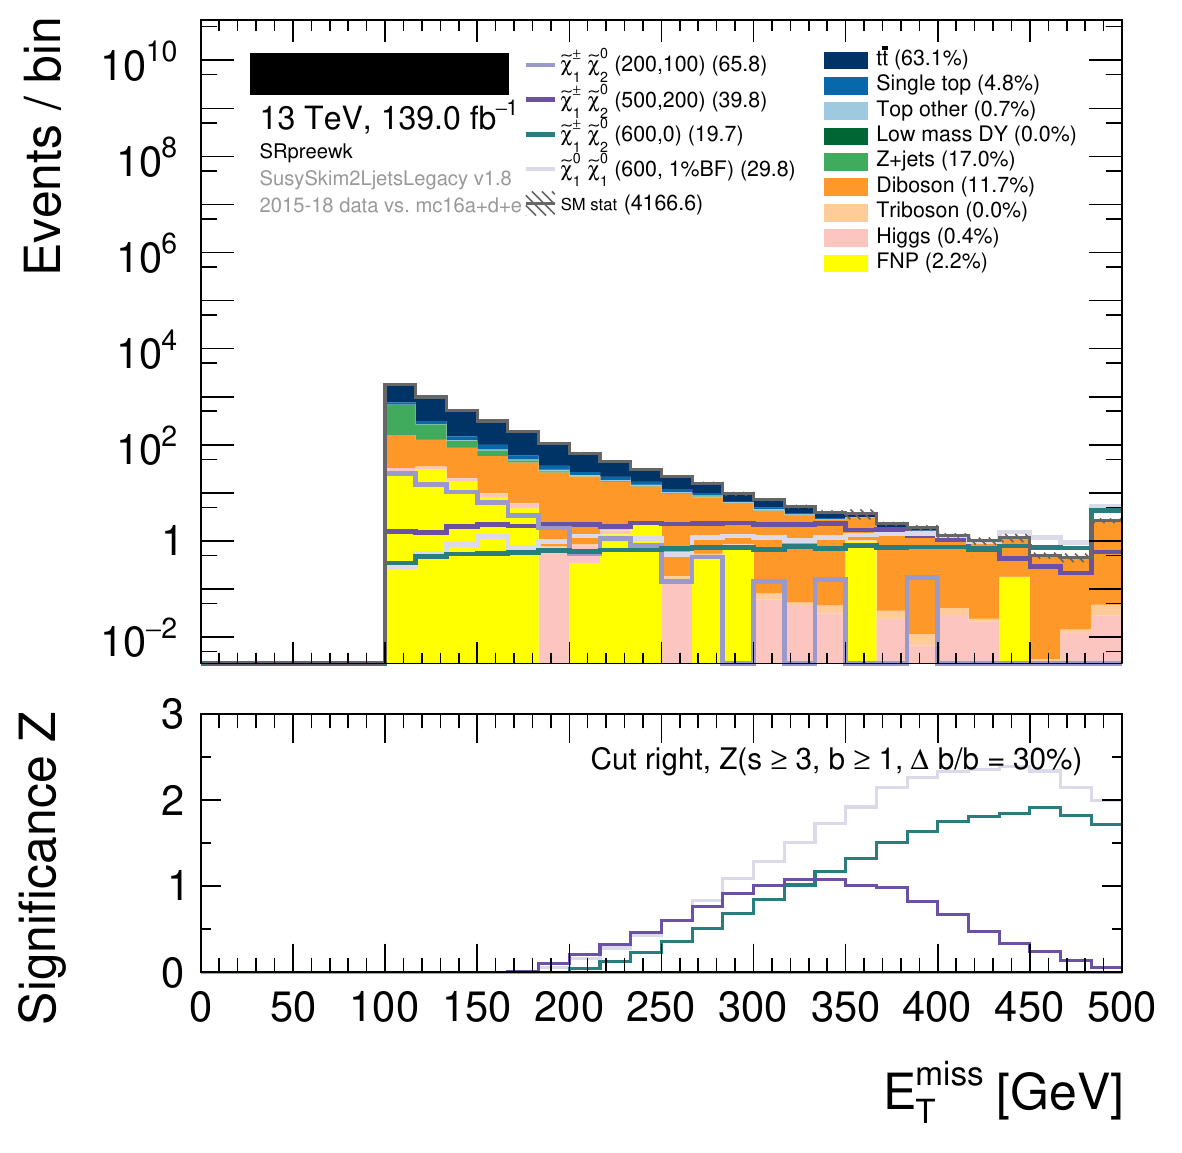
\includegraphics[width=0.48\textwidth]{figures/2ljets_presel_met_logy.png}
\hfill
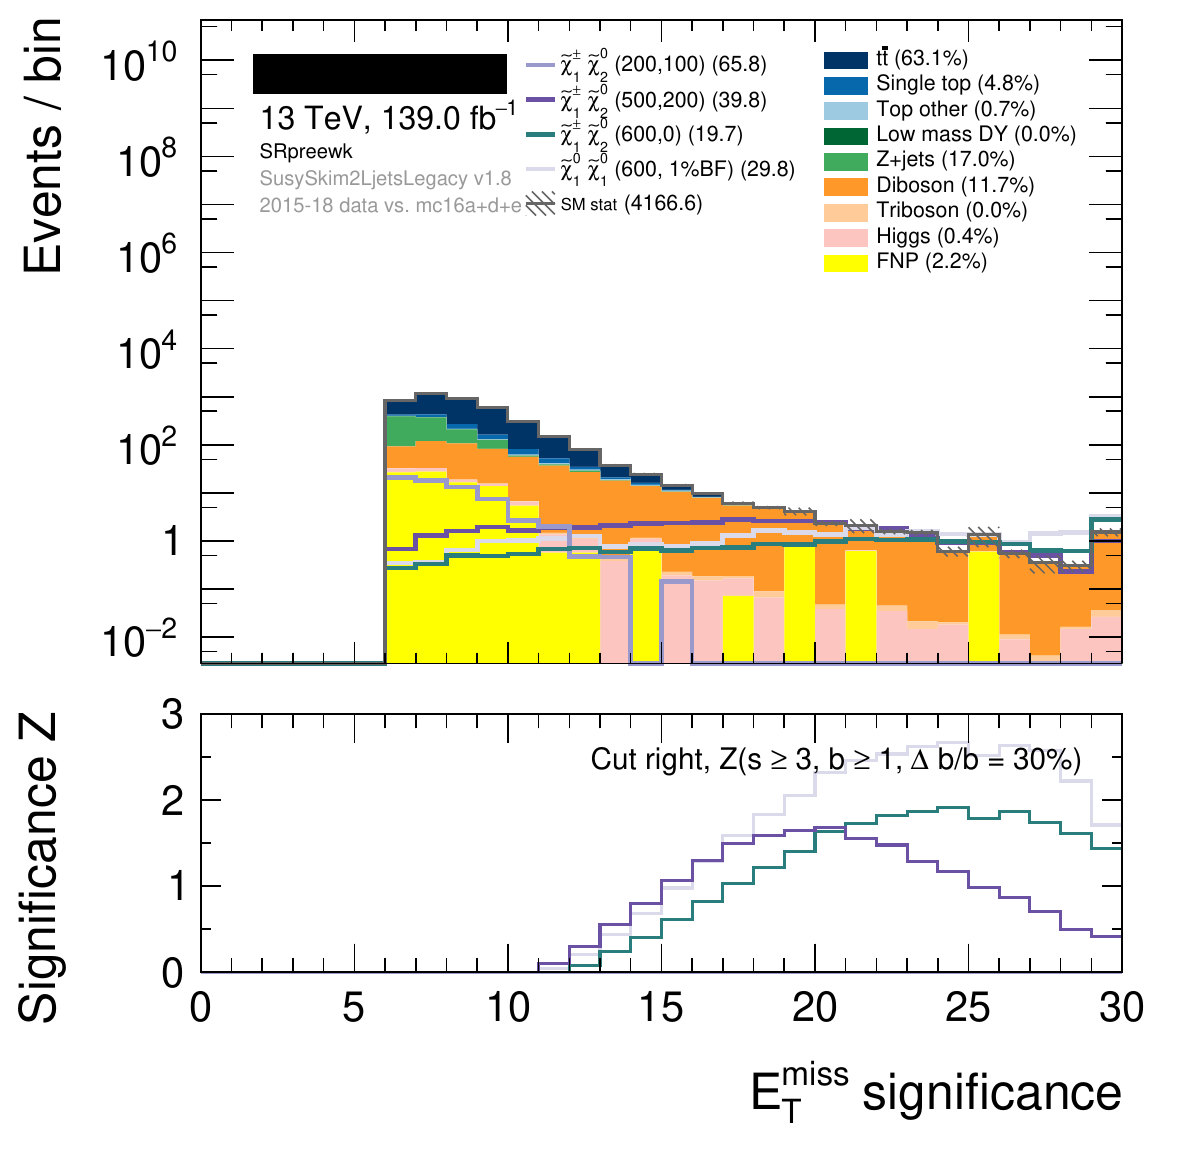
\includegraphics[width=0.48\textwidth]{figures/2ljets_presel_met_sig_logy.png}
\caption[
Illustration of how $\metsig$ beats $\met$ in sensitivity to example signal
models
]{
Illustration of how $\metsig$ beats $\met$ in sensitivity to example signal
models.
At large $\metsig$, $\ttbar$ and other backgrounds are suppressed, leaving
quite pure \diboson\ backgrounds and greater significance measures.
Signal models with smaller mass-splittings tend to have the bulk of their
events at smaller $\met$.
\\[0.5em]
This selection requires two same-flavour opposite-sign signal leptons with
$\pt^{\ell_2} > 25\,\eV[G]$,
$\mll \in (71, 111)\,\eV[G]$,
$\mjj \in (60, 110)\,\eV[G]$,
$\nbtag \leq 1$,
$\met > 100\,\eV[G]$, and
$\metsig > 6$.
\\[0.5em]
``Significance'' displayed in the lower subplot uses the Binomial significance
$Z_{Bi}$ from~\cite{cousins2008evaluation}, with a $30\%$ background
uncertainty and yields taken to the right of a given value.
Large values indicate expected sensitivity to the signal model.
}
\label{fig:2ljets_presel_met}
\end{figure}

Uncertainty in $\ptmiss$ is modelled for $\metsig$ by a covariance matrix
$\Sigma$ in the transverse plane, and used to define
\begin{equation}
\metsig^2
=
\ptmiss \Sigma^{-1} \ptmiss
=
\frac{(\met)^2}{\sigma_L^2(1 - \rho_{LT}^2)}
,
\end{equation}
in which $\sigma_L^2$ is the variance in the direction of $\ptmiss$ and
$\rho_{LT}$ is the correlation coefficient between the parallel and
perpendicular components~\cite{atlas_met_significance}.
This is the square of a Mahalanobis (standard-deviations) distance between
the origin and $\ptmiss$~\cite{mahalanobis1936generalised}.

Just as $\ptmiss$ is constructed from a (negative) sum of contributions from
objects in an event,
$\Sigma$ is a sum of covariances assigned to those objects;
both means and variances add linearly.


\subsection{\texorpdfstring{$\mttwo$}{mT2}}
\label{sec:2ljets_mt2}
Just as the slepton is a supersymmetric partner to a lepton, the `stransverse'
mass $\mttwo$ is a partner to the `transverse mass' $m_T$
(to be defined shortly),
that is useful in searches for supersymmetric particles.

The stransverse mass of an event is a greatest lower bound on the mass of a
pair-produced resonance, that applies when each partner decays semi-invisibly.
For example, an on-shell $\tilde\ell^+\tilde\ell^-$ pair decaying as
$\tilde\ell^+ \rightarrow \ell^+ \neutralino_1
,~
\tilde\ell^- \rightarrow \ell^- \neutralino_1$ has
$\mttwo(\ell^+, \ell^-, m(\neutralino_1)) \leq m(\tilde\ell)$, plus some error
margin for experimental resolution.
Such cases are common, since R-parity conservation implies pair production,
and the idea that dark matter could comprise the lightest supersymmetric
particle motivates invisible decays.

Lacking direct observation of sleptons, $\mttwo$ remains useful in separating
standard model processes; dileptonic $\ttbar$ and $W^\pm W^\mp$ decays both
satisfy $\mttwo(\ell^+, \ell^-, 0) \leq m(W)$ (since $0 \approx m(\nu)$).
The $\twoljets$-electroweak search depends on this effect;
most selections require $\mttwo(\ell^+, \ell^-, 0) > 80\,\eV[G]$, or similar,
to reduce $\ttbar$, $W^\pm W^\mp$ and $\tau^\pm\tau^\mp$ backgrounds.

To be precise, the stransverse mass explores how to split the observed
$\ptmiss$ between the two visible decay products in an event, and can be
defined as
\begin{equation}
\mttwo(a_\mu, b_\mu, m)
=
\min_{\vec p + \vec q=\ptmiss}
\max
\begin{Bmatrix}
m_T(a_\mu + \{\!\sqrt{m^2 - \vec p_T^{\:2}},\,\vec p\,\}_\mu)\\
m_T(b_\mu + \{\!\sqrt{m^2 - \vec q_T^{\:2}},\,\vec q\,\}_\mu)\\
\end{Bmatrix}
,
\end{equation}
in which $m_T^2(p_\mu) = p_0^2 - p_1^2 - p_2^2$ and $\{E,\,\vec p\,\}_\mu$ denotes
the four-vector with energy $E$ and momentum $\vec p$~\cite{lester1999measuring}.
As an extension, one can assign different masses $m_p$ and $m_q$ to
the two invisible products~\cite{lester2015bisection}.

Numerical evaluation of $\mttwo$ can be performed efficiently with interval
bisection algorithms, which seek the least resonance mass for which the
transverse masses allow any compatible assignment which also satisfies
$\vec p + \vec q = \ptmiss$.
Testing this compatibility reduces to testing for the intersection of two
ellipses, one for each transverse
mass~\cite{cheng2008minimal, lester2015bisection}.

Public code for calculating $\mttwo$ is available in a Python
library~\cite{gillam2021mt2}, to which I contributed a faster and more robust
implementation of the bisection algorithm by
Lester and Nachman~\cite{lester2015bisection} during this project.


\subsection{Jet pairs}
Di-jet assignments, for variables like $\mjj$ and $\rjj$, are always chosen as
the two hardest jets.
Why?

This choice matches the convention of SR2-int and SR2-high from the previous
search~\cite{atlas_23l_SUSY_2016_24}, but my initial reaction was that since we
are looking for jet pairs near to $m(W)$ or $m(Z)$, we should surely choose
candidate jet pairs by their mass.

Two alternative di-jet assignments were therefore considered in early
development of region designs:
the two jets with invariant mass closest to $m(W)$, and the two jets with the
minimum $\rjj^\mathrm{alternative}$ between them.
The result was bland.
All assignments performed similarly, and all left similar fractions of signal
yields outside the mass window.
The simplicity and precedent for the two-hardest jet assignment therefore swung
the decision.

However, alternatives did select different subsets of signal yields;
the alternative jet assignments had some potential to define secondary signal
regions to catch those signal events which fall outside the primary
$\mjj$ window.
One can, for example, select $\mjj \notin 60\textrm{--}110\,\eV[G]$ and
$\mjj^\mathrm{alternative} \in 60\textrm{--}110\,\eV[G]$ for some additional
sensitivity.
However, this comes at the cost of complexity, particularly in the boundaries
with control and validation regions, and is therefore not used here.


\subsection{Cheat-sheet}
Uncomfortably many event variables are used to define the regions of this
analysis.
To aid future revision of their meanings, definitions, and references for these
variables are collected here.
All dimensionful quantities are in $\eV[G]$.
\begin{itemize}
\item $\met$: missing transverse momentum
\item $\metsig$: object-based missing transverse momentum significance;\\
described in Section~\ref{sec:2ljets_metsig}
\item $\ptjone$: transverse momentum of the hardest jet%
\vspace{0.5em}
\item $\mll$: invariant mass of the hardest two leptons
\item $\mjj$: invariant mass of the two hardest jets
\item $\mbb$: invariant mass of the two hardest $b$-tagged jets
\item $\mjetone$: mass of the hardest jet
\item $\mttwoll$: `stransverse' mass of the lepton pair with massless invisibles;\\
described in Section~\ref{sec:2ljets_mt2}
\vspace{0.5em}
\item $\rll$: distance in $\eta\textrm{--}\phi$ between the lepton pair
\item $\rjj$: distance in $\eta\textrm{--}\phi$ between the two hardest jets%
\vspace{0.5em}
\item $\njet$: number of signal jets
\item $\nbtag$: number of b-tagged jets;
described in Section~\ref{sec:2ljets_btagging}
\vspace{0.5em}
\item $\dphillmet$: azimuthal angle between the lepton pair and $\ptmiss$
\item $\dphijmet$: azimuthal angle between the hardest jet and $\ptmiss$
\end{itemize}
All of these are physical properties of particles or collections of particles.
Please remember that none is an exact or true value;
all are estimates based on approximate reconstructions.
While this distinction is easy to drop in lax language, it is necessary to
understand the shapes of noisy variables such as $\mjj$ and indeed the
existence of $\metsig$.


\FloatBarrier
\section{Design}
\label{sec:2ljets_design}
Perhaps the most impactful decision in a search is the design of its regions.
Like most decision, these designs must be made to balance conflicting and
vaguely-specified desires, and are informed with incomplete information.

My understanding of search design is as conflict between simplicity and
precision.
Yes, an extra bin with higher $\metsig$ might catch some extreme signals,
and yes, an RJR construction might pick out candidate decay trees without
extreme $\met$.
But if these delay the result without comparable benefits, they will act to
slow down our scientific progress.

Furthermore, simplicity encourages interpretability and trust.
A selection at $100\,\eV[G]$ may be slightly outperformed in precision by one
at $100.314\,\eV[G]$, but the former is preferable --- it is easily
communicated and perhaps understood or reproduced by readers.
The latter could be overly tuned, perhaps by a learning algorithm, to specific
simulations.
Perhaps it cut out a highly weighted sample which, although annoying, was an
honest representation of our modelling.
Restricting ourselves to round numbers not only clarifies our communications,
but keeps us honest by denying ourselves the ability to over-fit simulations.

Numerical simplicity is valuable.
I wrote in a draft of our \atlas-internal documentation that numerical
simplicity was a design goal, but am guilty of removing that statement after a
senior reviewer suggested that it was ``too honest''.
% ~\cite{comment2020toohonest}. % Could cite, probably should not.

The remainder of this section describes the designs of the control,
validation, and signal regions of the $\twoljets$ analysis, along with some
reasoning behind those designs.

\begin{figure}[tp]
\centering
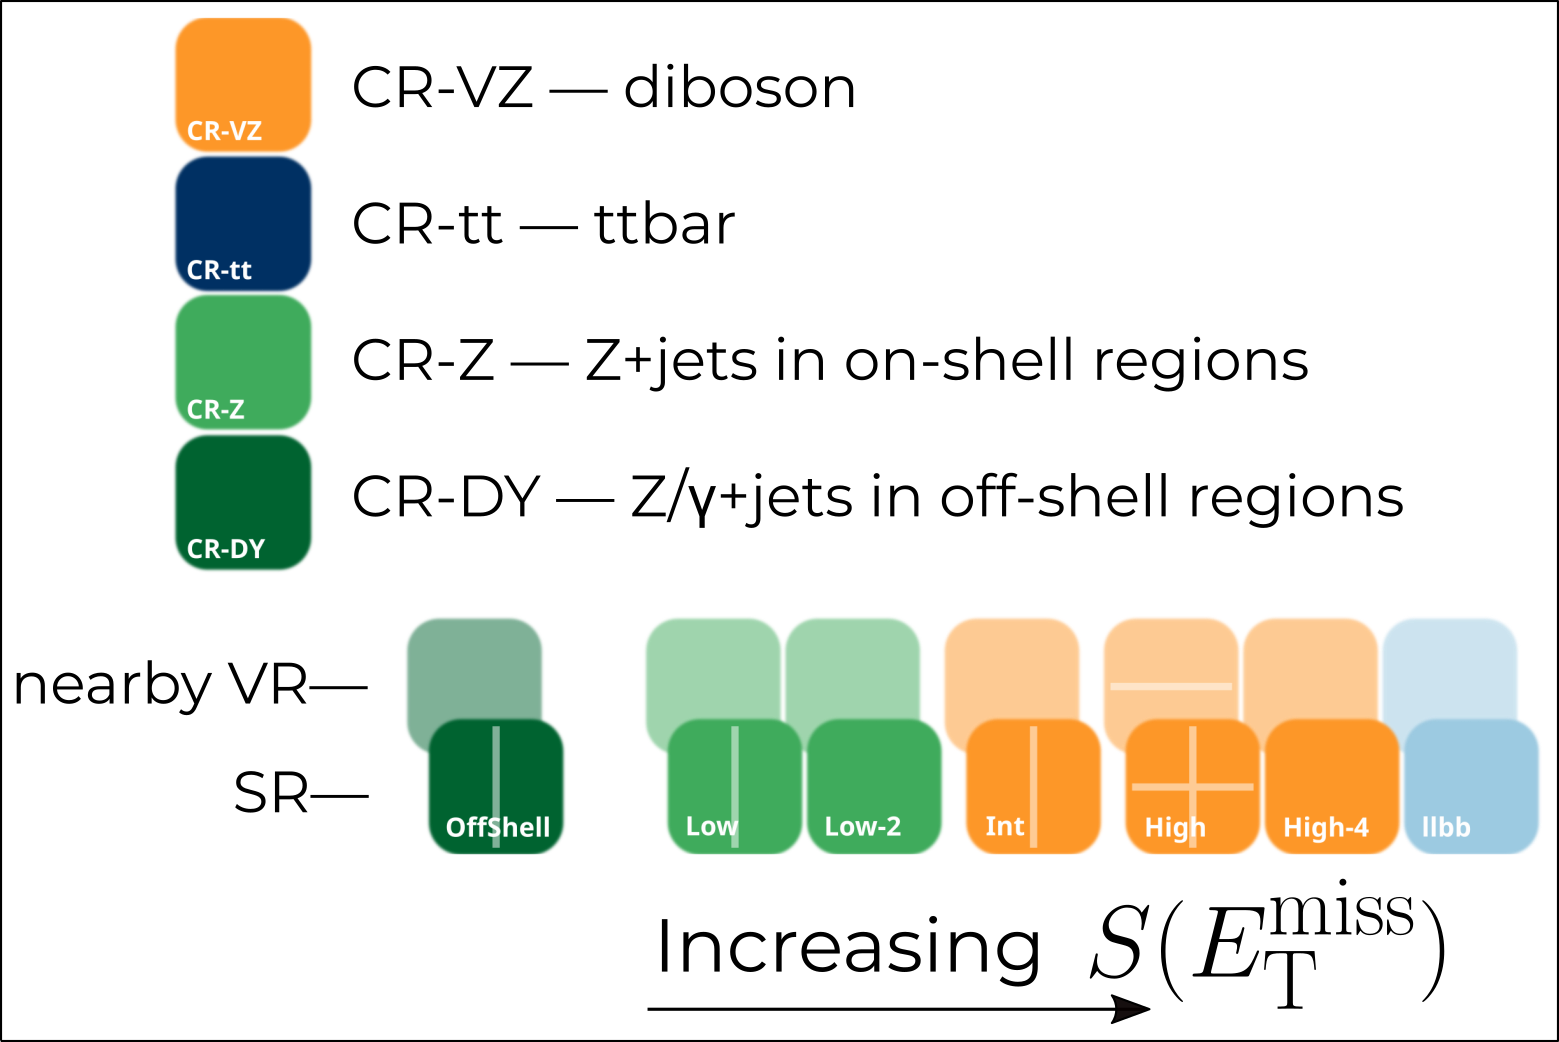
\includegraphics[width=0.99\textwidth]{figures/2Ljets_pam_ewkslide.png}
\caption[
Region design summary slide
]{%
Region design summary slide adapted from an internal presentation.
Colours represent primary background contributions in our plotting scheme.
}
\label{fig:2ljets_region_summary}
\end{figure}

The clearest idea behind this design is to split regions on $\metsig$.
Motivation for this design is displayed in
Figure~\ref{fig:2ljets_presel_met};
$\metsig$ does better than $\met$ in separating background and signal
contributions for models with various mass splittings above $m(Z)$.
Furthermore, $\metsig$ also works to separate signal models from each other;
signals with larger mass differences in their decays to invisibles tend to have
larger $\metsig$.
Binning regions in $\metsig$ therefore also improves sensitivity to
individual parameter points and allows targeted selections on other,
locally-relevant, event variables.

Regions in three blocks of $\metsig$ are named High, Intermediate (or Int),
and Low,
which target models with decreasing mass splittings and lepton pairs on the
$Z$ resonance mass.
Separate regions target $\mll < m(Z)$ for models with small mass splittings,
which force decays to proceed via low-mass off-shell weak bosons.

Following the conventional style described in
Section~\ref{sec:searches_searches},
control regions are defined to normalize specific background samples,
and validation regions are defined to test their extrapolation towards
signal regions before unblinding.

All regions are defined within a loose `Pre-selection' requirement which
requires the basic $Z\rightarrow \ell^+\ell^-$ plus jets plus $\met$
conditions that we target in the $\twoljets$-electroweak.
These Pre-selection requirements are defined in Table~\ref{tab:2ljets_presel}.

\begin{table}[tp]
\centering
\begin{tabular}{c}
Pre-selection:
\\[1em]
$n_\mathrm{leptons}^\mathrm{signal} = n_\mathrm{leptons}^\mathrm{baseline} = 2$
\\[0.5em]
same flavour, opposite charge leptons
\\[0.5em]
$\njet \geq 1$
\\[0.5em]
$p_\mathrm{T}^{\,\ell_2} > 25$
\\[0.5em]
$\metsig > 6$
\\[0.5em]
$\met > 100$
\end{tabular}
\caption[%
Pre-selection requirements ensured prior to all region definitions in the
$\twoljets$-electroweak search
]{%
Pre-selection requirements ensured prior to all region definitions in the
$\twoljets$-electroweak search.
Although $\metsig > 6$ implies that most events already have large $\met$
$\met > 100\,\eV[G]$ requirement is included to ensure that events with small
$\met$ and smaller uncertainties on it are excluded.
}
\label{tab:2ljets_presel}
\end{table}

High regions are discussed in Section~\ref{sec:2ljets_high}.
Intermediate regions are discussed in Section~\ref{sec:2ljets_int}.
Low regions are discussed in Section~\ref{sec:2ljets_low}.
Off-shell regions are discussed in Section~\ref{sec:2ljets_high}.
Control and validation regions are included in these sections near to their
targetted regions.
Finally, how these are combined into `Discovery' regions for
model-independent interpretations is discussed in
Section~\ref{sec:2ljets_disco}.

A high-level summary of the region design is shown in
Figure~\ref{fig:2ljets_region_summary}.
The design comprises four control regions and thirteen orthogonal signal region
bins, with validation regions targeting each group of signal regions.

\emph{%
Thanks are due to Knut~Vadla for important contributions in the initial
exploration of signal region designs,
to Ben Hooberman for suggesting the investigation of massive jets,
and to both, and the whole $\twoljets$, collaboration in their finalization.
}

% presel table should come before High
\FloatBarrier
\subsection{High}
\label{sec:2ljets_high}
The highest $\metsig$ selections, of around $\metsig > 18$, contain almost pure
\diboson\ backgrounds in relatively small quantities, along with the bulk masses
of signal samples at the heaviest resonance masses.
This is therefore the most promising territory for signal regions which are
highly sensitive to the most extreme signals.
Their backgrounds, however, must be constrained by control regions in less
extreme parameter spaces with more data.

Diboson backgrounds and C1N2 signals have more in common than just $\met$.
Notably, both also produce resonant $Z\rightarrow \ell^+\ell^-$ pairs
and do not enhance the rate of heavy-flavour jets, as displayed in
Figure~\ref{fig:2ljets_high_mll_b}.
Since signals and backgrounds have such similar shapes in $\mll$ and $\nbtag$,
sensitivity is only decreased by rejecting portions of these distributions.
Although most $\twoljets$-electroweak regions use tighter selection on these
variables to reduce backgrounds, this observation allows us to win
additional sensitivity in High regions by loose requirements.

The high regions, defined in Table~\ref{tab:2ljets_high}, comprise SR-High,
SR-High-1J, and \srllbb.

\begin{table}[tp]
\centering
\begin{tabular}{lccccc}
& $\njet$
& $\nbtag$
& $\metsig$
& $m_*$
& $\rjj$
\\[1em]
SR-High
& $\geq2$
& $\leq 1$
& $18\textrm{--}21\textrm{--}\infty$
& $\mjj\!:~  60\textrm{--}110$
& $0\textrm{--}0.8\textrm{--}1.6$
\\[0.5em]
\: VR-High
& $\geq2$
& $\leq 1$
& $> 18$
& $\uwave{\mjj\!:~  20\textrm{--}60 \mid 110\textrm{--}\infty}$
& $< 1.6$
\\[0.5em]
\: VR-High-R
& $\geq 2$
& $\leq 1$
& $> 18$
& $\uwave{\mjj\!:~  > 20}$
& $\uwave{> 1.6}$
\\[1em]
SR-High-1J
& $\hphantom{\geq}~1$
& $\leq 1$
& $> 12$
& $\mjetone\!:~  60\textrm{--}110$
&
\\[0.5em]
\: VR-High-1J
& $\hphantom{\geq}~1$
& $\leq 1$
& $> 12$
& $\uwave{\mjetone\!:~  20\textrm{--}60 \mid 110\textrm{--}\infty}$
&
\\[1em]
\srllbb
& $\geq 2$
& $\geq 2$
& $> 18$
& $\mbb\!:~  60\textrm{--}150$
&
\\[0.5em]
\: VR-$\llbb$
& $\geq 2$
& $\geq 2$
& $\uwave{12\textrm{--}18}$
& $\mbb\!:~  60\textrm{--}150$
&
\end{tabular}
\\[1em]
Common: Pre-selection,
$\mll \in 71\textrm{--}111$, and
$\mttwoll > 80$.
\caption[
High region definitions in the $\twoljets$-electroweak analysis
]{%
High region definitions in the $\twoljets$-electroweak analysis.
En-dashes `$a\textrm{--}b$' indicate open intervals $(a, b)$.
Concatenated intervals `$a\textrm{--}b\textrm{--}c$' indicate binning
with boundaries at $a$, $b$, and $c$.
The mid-bar `$\mid$' indicates logical or.
Differences between regions are \uwave{underlined}.
\\[0.5em]
The $\rll$ bins of SR-High are labelled SR-High-8 and SR-High-16, and their
$\metsig$ bins are suffixed -a and -b for $\metsig \in 18\textrm{--}21$
and $\metsig > 21$ respectively.
}
\label{tab:2ljets_high}
\end{table}

\begin{figure}[tp]
\centering
\begin{subfigure}{0.48\textwidth}
\centering
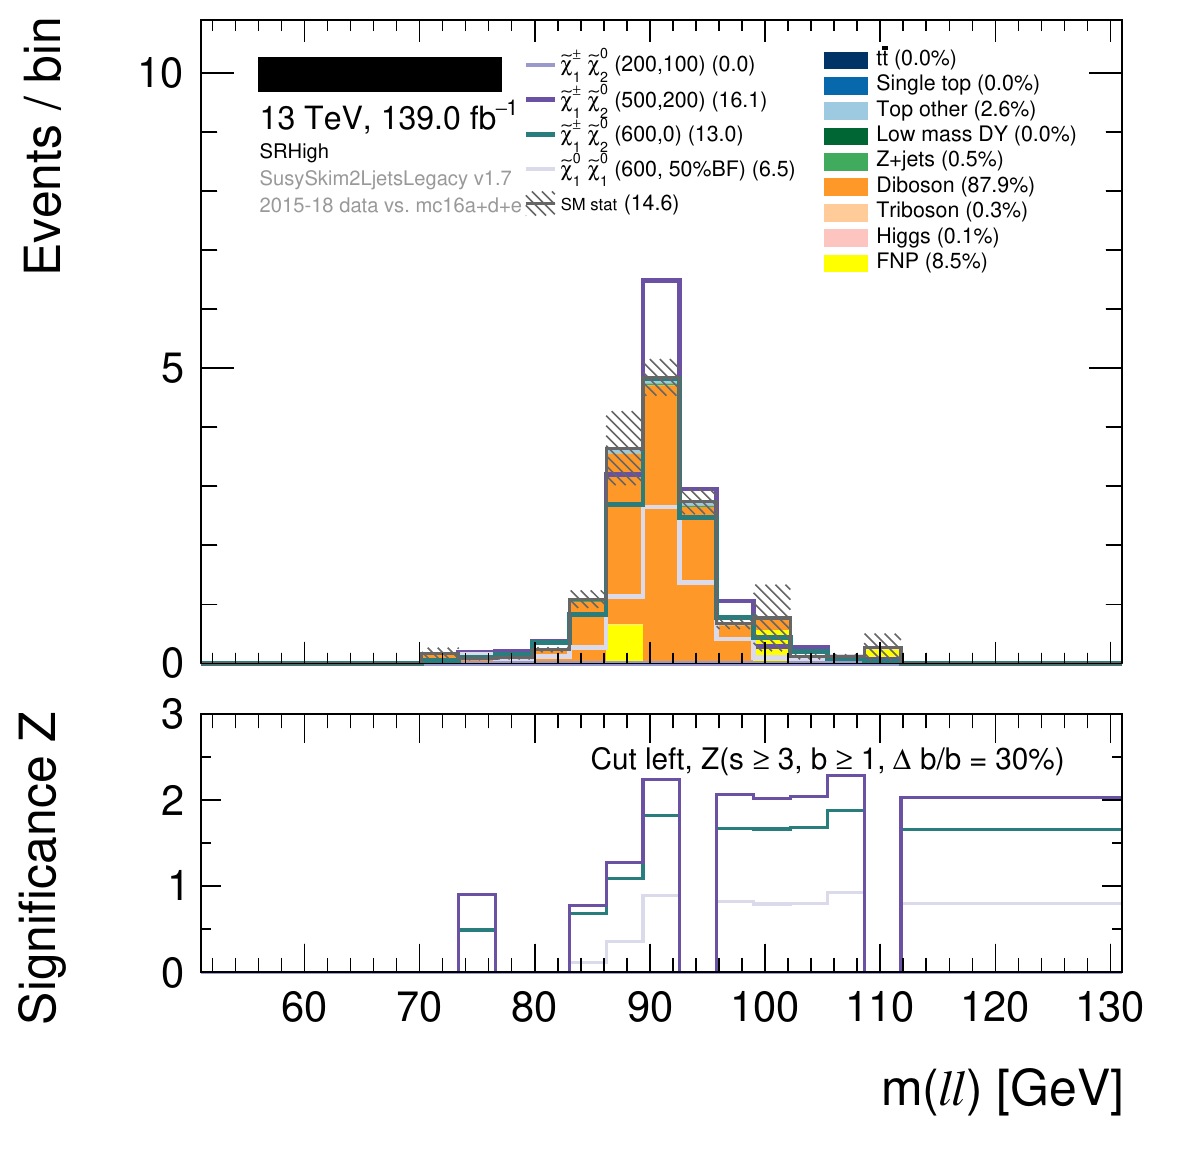
\includegraphics[width=\textwidth]{figures/2ljets_region_design_hist1d_mll_SRHigh.png}
\caption{SR-High, $\mll$}
\end{subfigure}
\hfill
\begin{subfigure}{0.48\textwidth}
\centering
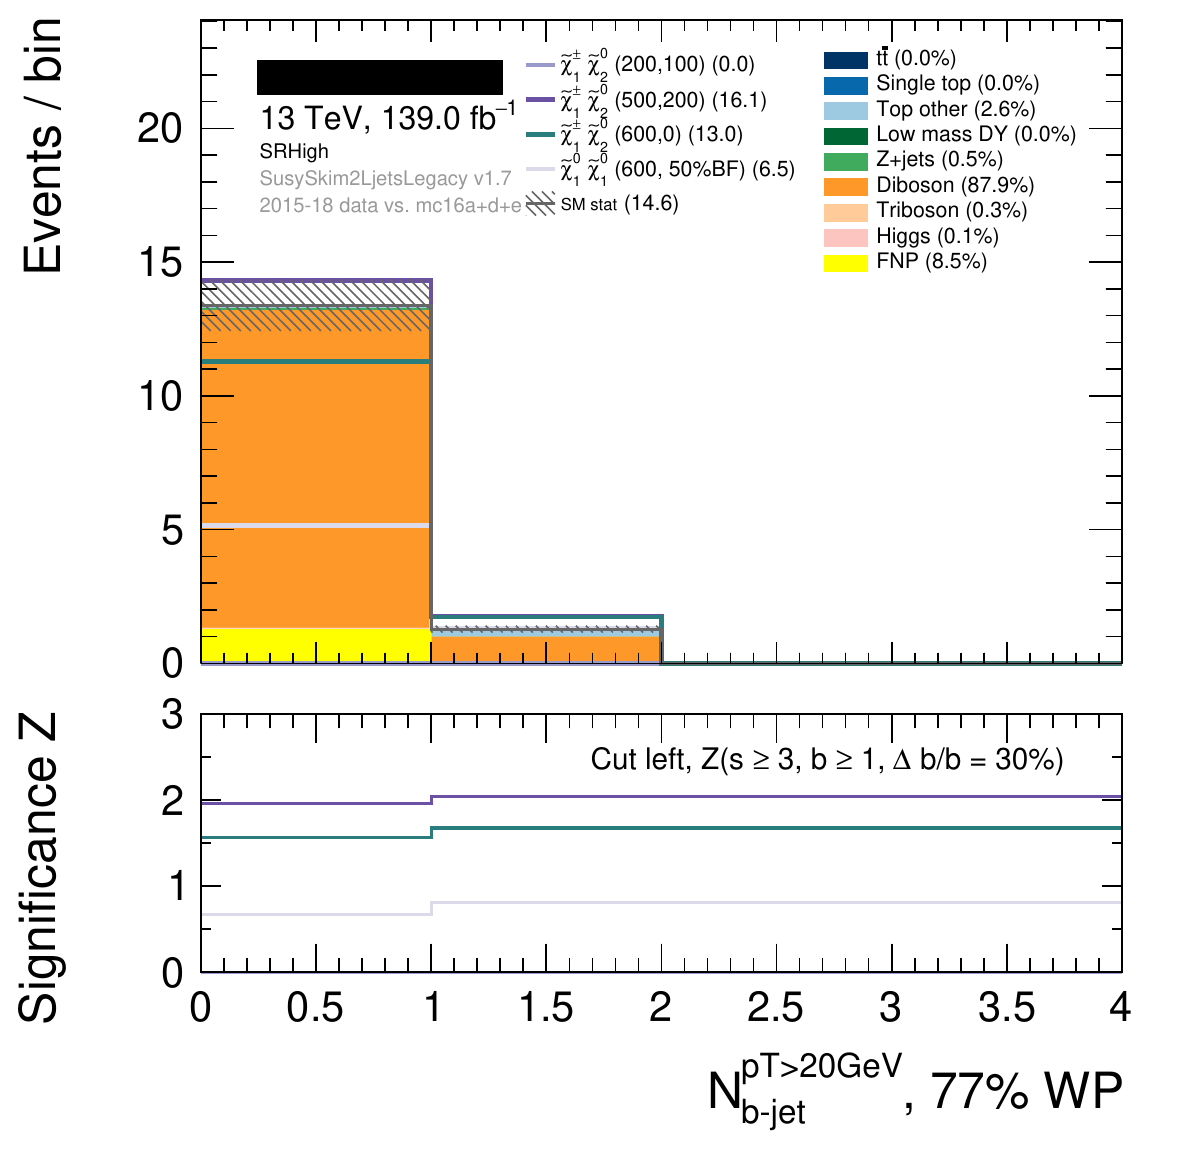
\includegraphics[width=\textwidth]{figures/2ljets_region_design_hist1d_nbtag_SRHigh.png}
\caption{SR-High, $\nbtag$}
\end{subfigure}
\caption[
SR-High with relaxed selections on (a) $\mll$ or (b) $\nbtag$
]{%
SR-High with relaxed selections on (a) $\mll$ or (b) $\nbtag$.
The pure \diboson\ background has very similar shapes to the signals.
Tighter cuts would therefore reduce background and signal yields comparably,
reducing sensitivity.
The significance dropouts in (a) are errors in plotting.
`Significance Z' is the binomial significance~\cite{cousins2008evaluation}
with a $30\%$ relative background uncertainty.
Error bars are statistical.
}
\label{fig:2ljets_high_mll_b}
\end{figure}

The $\mll \in 71\textrm{--}111$ window loosely selects the $m(Z)$ peak to
scoop up nearby rare or mismeasured events.
Similarly, allowing up to one $b$-tag improves yields without boosting
backgrounds, since the $\metsig$ requirement already removes most $\ttbar$
processes.

The standard wide $\mjj \in 60\textrm{--}110\,\eV[G]$ requirement captures
both $W\rightarrow jj$ and $Z\rightarrow jj$ for C1N2 and GMSB models
respectively.

As explained in Section~\ref{sec:2ljets_mt2}, requiring $\mttwo$ above $m(W)$
effectively removes $\ttbar$ and other backgrounds.
The relatively low requirement $\mttwoll > 80\,\eV[G]$ is chosen here and
elsewhere in the $\twoljets$-electroweak design to reduce these backgrounds
while minimize lost signal yields.

To maximize projected sensitivity, SR-High is split into four bins with
one split at $\rjj = 0.8$, to form SR-High-8 and SR-High-16, and a second at
$\metsig = 21$ to split these into SR-High-*-a and SR-High-*-b.
For example, SR-High-8-b requires $\rjj < 0.8$ and $\metsig > 21$.
The regions SR-High-8 and SR-High-16 are displayed in
Figure~\ref{fig:2ljets_high_region}, with their -a and -b bins visible across
the $\metsig$ distribution.

\begin{figure}[tp]
\centering
\begin{subfigure}{0.48\textwidth}
\centering
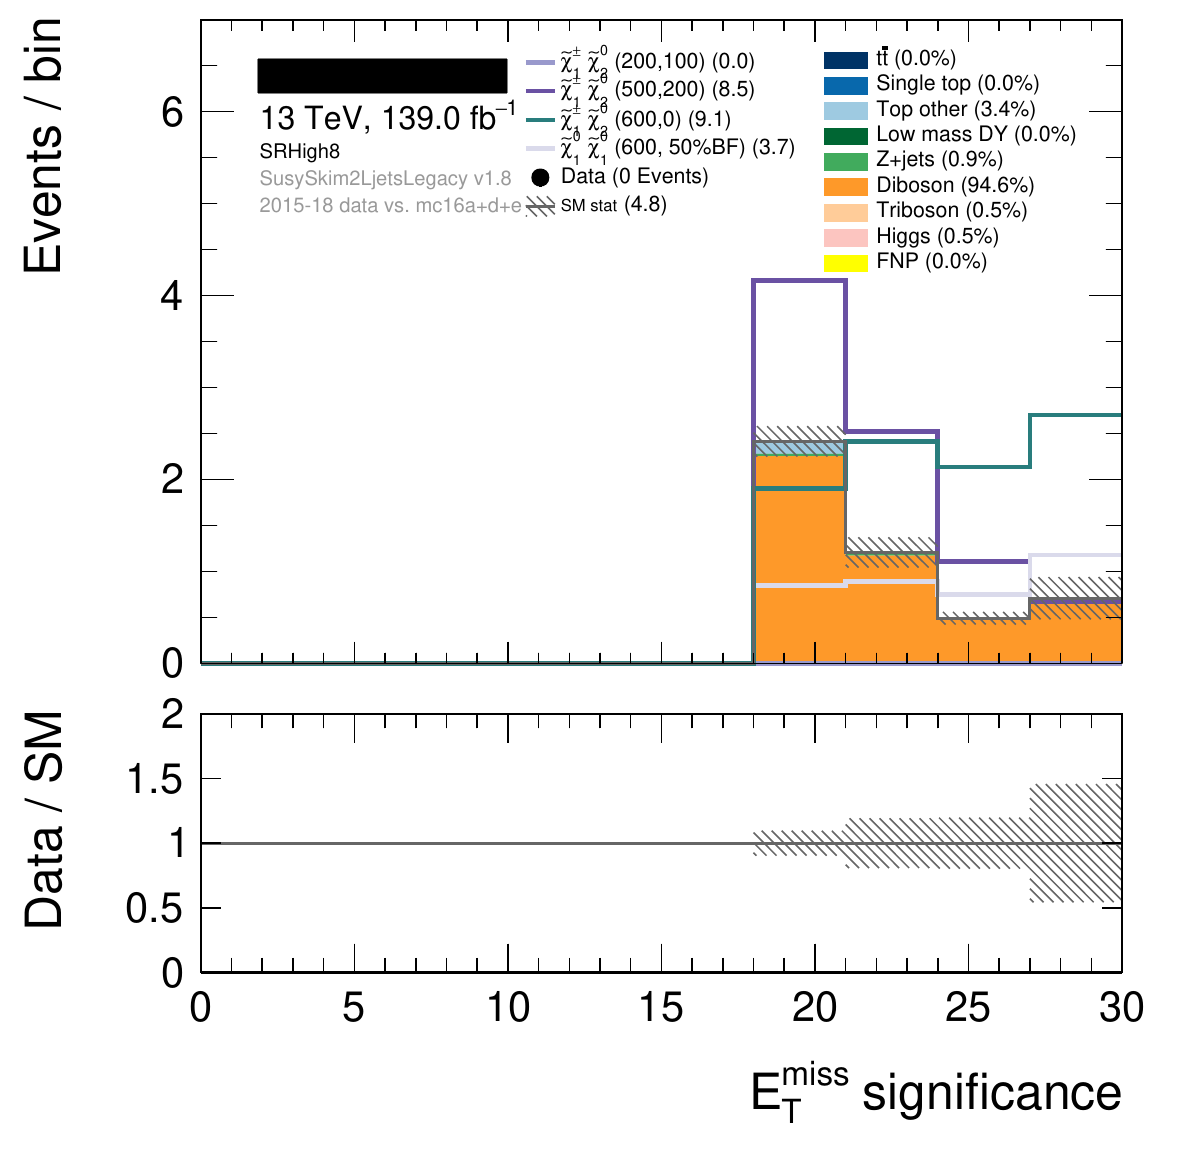
\includegraphics[width=\textwidth]{figures/2ljets_def_met_Sign_SRHigh8.png}
\caption{SR-High-8, $\metsig$}
\end{subfigure}
\hfill
\begin{subfigure}{0.48\textwidth}
\centering
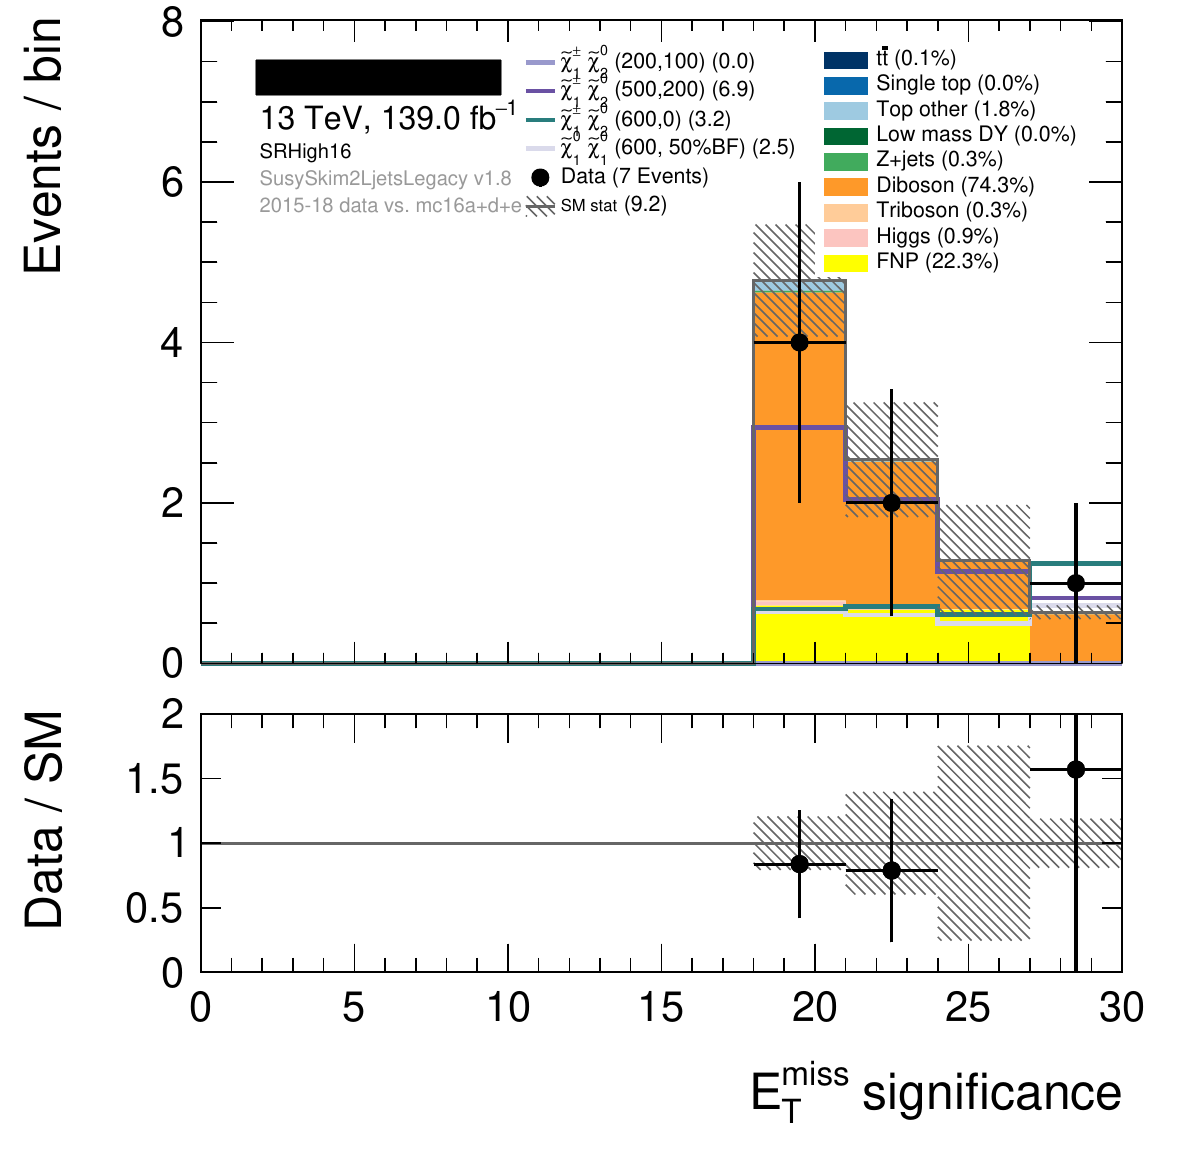
\includegraphics[width=\textwidth]{figures/2ljets_def_met_Sign_SRHigh16.png}
\caption{SR-High-16, $\metsig$}
\end{subfigure}
\\[0.5em]
\begin{subfigure}{0.48\textwidth}
\centering
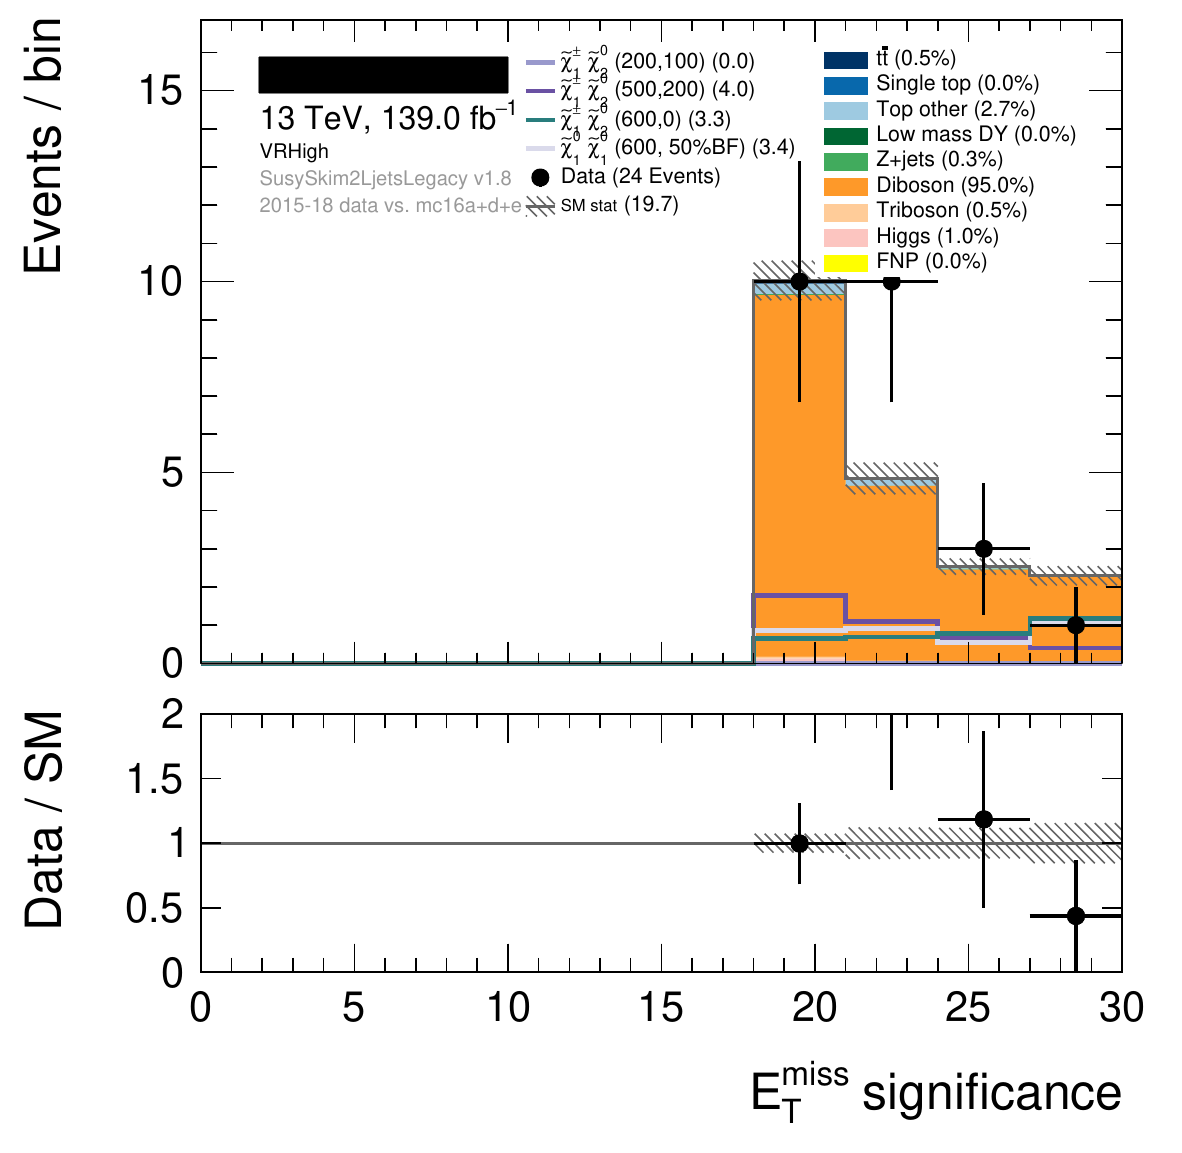
\includegraphics[width=\textwidth]{figures/2ljets_def_met_Sign_VRHigh.png}
\caption{VR-High-8, $\metsig$}
\end{subfigure}
\hfill
\begin{subfigure}{0.48\textwidth}
\centering
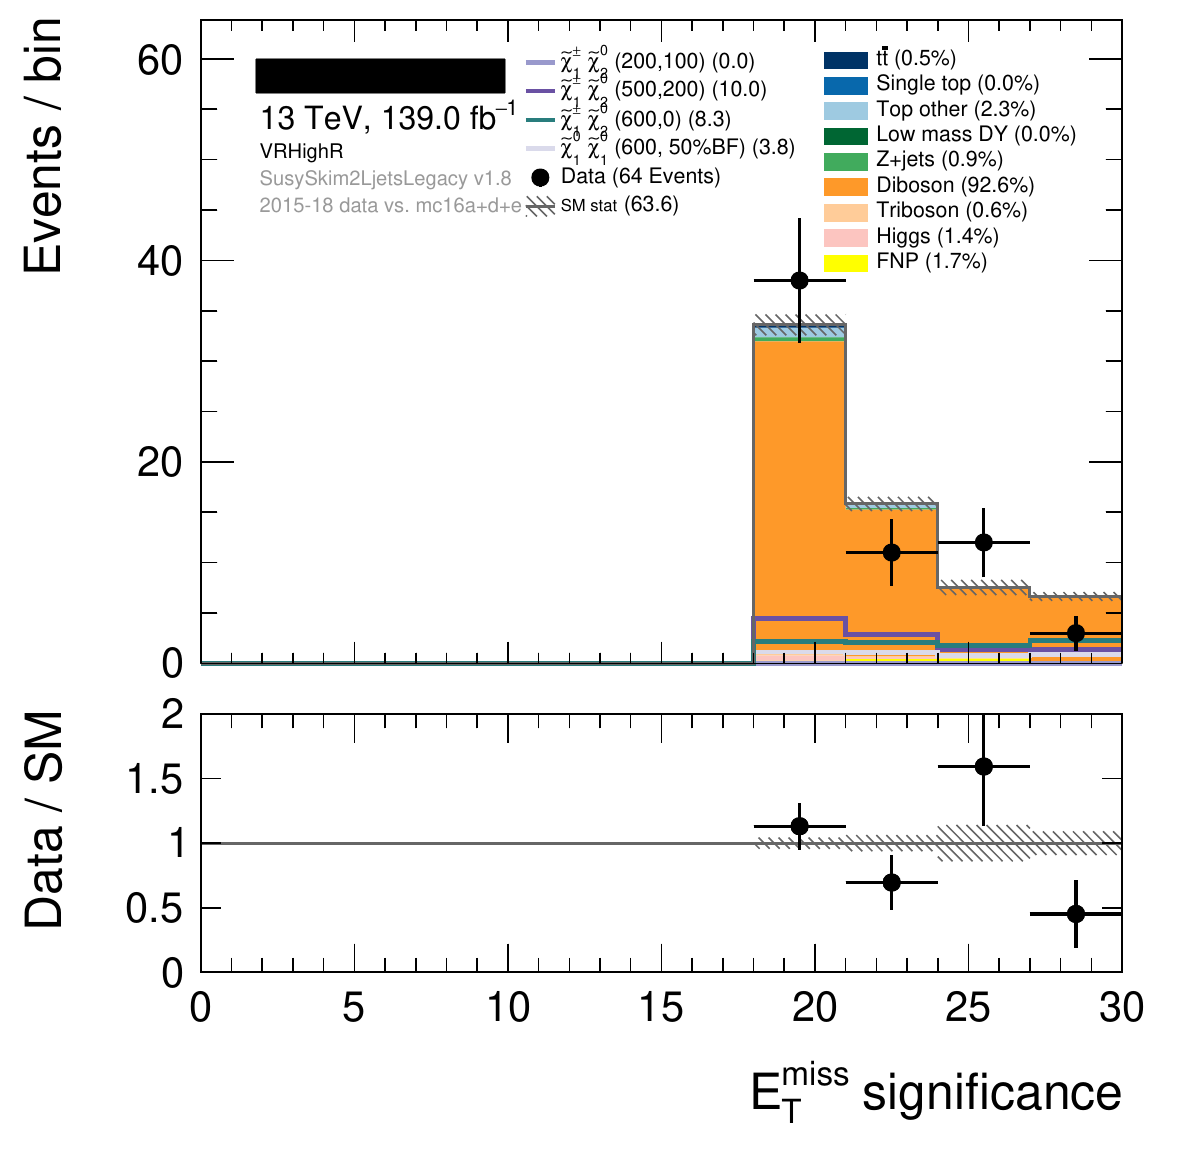
\includegraphics[width=\textwidth]{figures/2ljets_def_met_Sign_VRHighR.png}
\caption{VR-High-16, $\metsig$}
\end{subfigure}
\caption[
Pre-fit distributions of $\metsig$ in High signal and validation regions
]{%
Pre-fit distributions of $\metsig$ in High signal and validation regions.
Signal regions are unblinded.
Errors are statistical.
}
\label{fig:2ljets_high_region}
\end{figure}

One major difference between signals and \diboson\ backgrounds is that signal
jet pairs mostly arise from boosted $W\rightarrow jj$ decays, which more often
produce nearby jets.
Selecting small $\rjj$ in SR-High therefore picks out these boosted cases.

Extremely boosted $W$ bosons can be clustered into single jets.
Although large-radius jets are typically used to capture these, we only use
small, $R=0.4$, jets in the $\twoljets$ analysis.
And those small jets can work for the extreme boosts that our signals produce.
To catch these extreme events is the goal of SR-High-1J, which is displayed
in Figure~\ref{fig:2ljets_high_1J_region}.
The use of $\mjetone$ with small-radius jets for this region is unusual,
and required modelling of additional uncertainties that we discuss in
Section~\ref{sec:2ljets_jet_mass}.

\begin{figure}[tp]
\centering
\begin{subfigure}{0.48\textwidth}
\centering
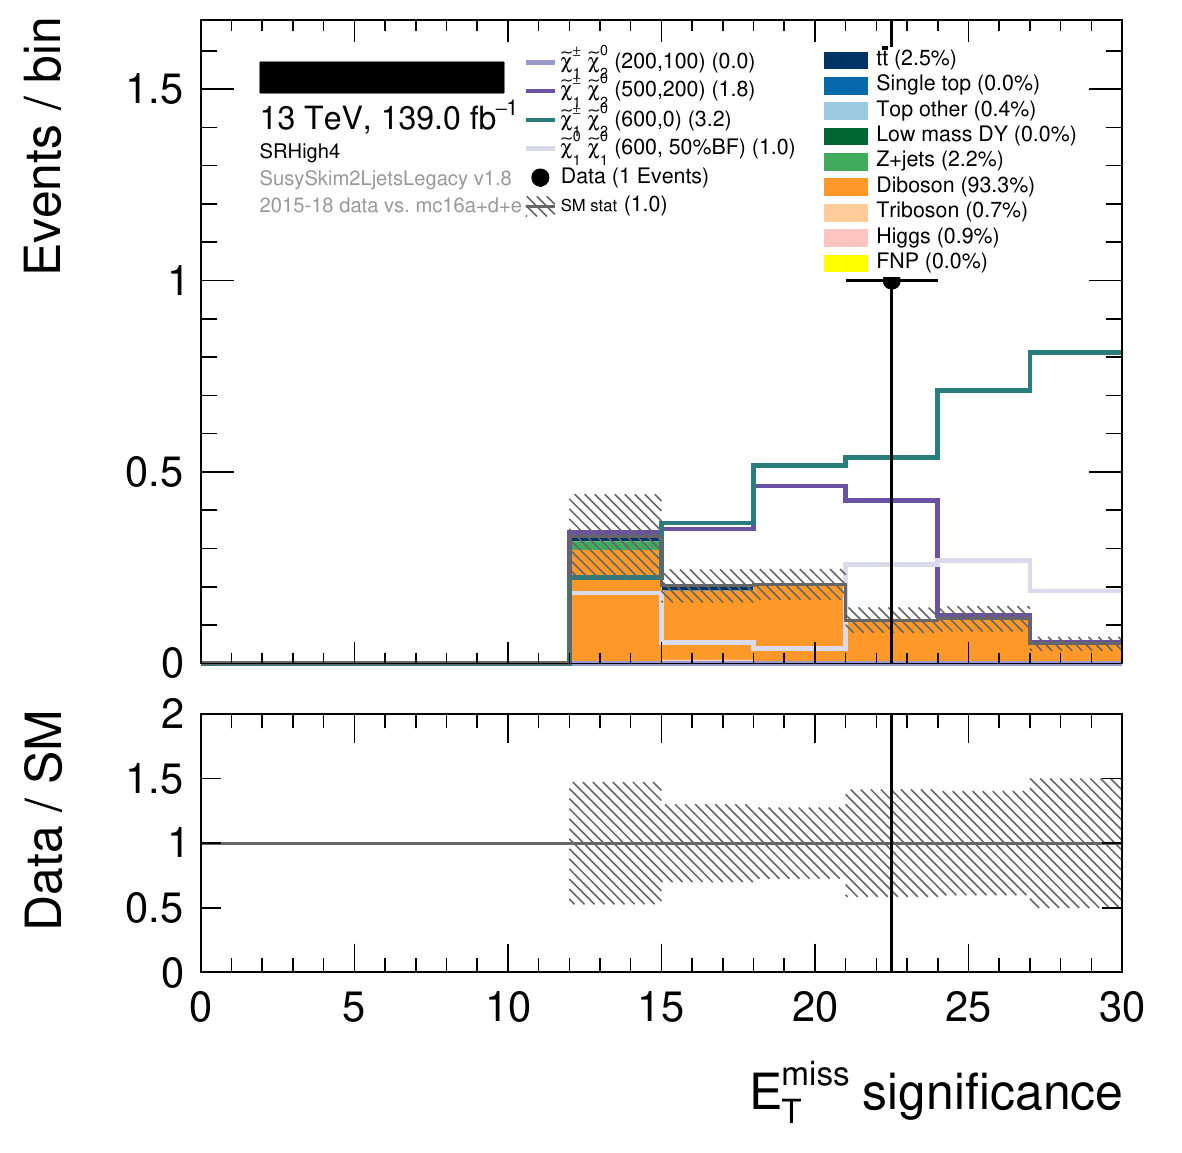
\includegraphics[width=\textwidth]{figures/2ljets_def_met_Sign_SRHigh4.png}
\caption{SR-High-1J, $\metsig$}
\end{subfigure}
\hfill
\begin{subfigure}{0.48\textwidth}
\centering
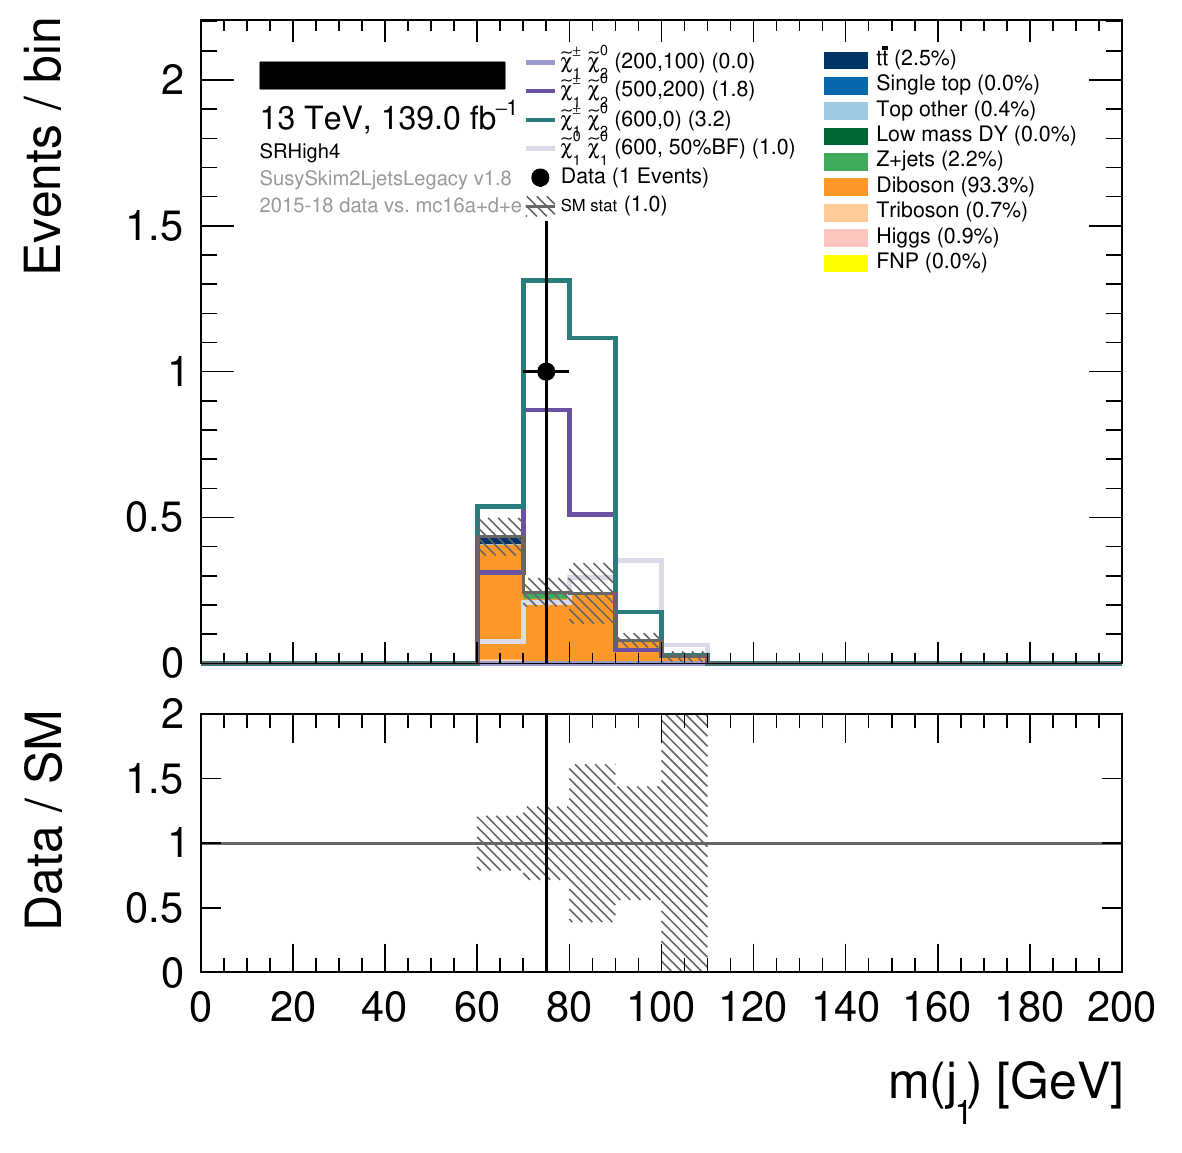
\includegraphics[width=\textwidth]{figures/2ljets_def_mjetone_SRHigh4.png}
\caption{SR-High-1J, $\mjetone$}
\end{subfigure}
\\[0.5em]
\begin{subfigure}{0.48\textwidth}
\centering
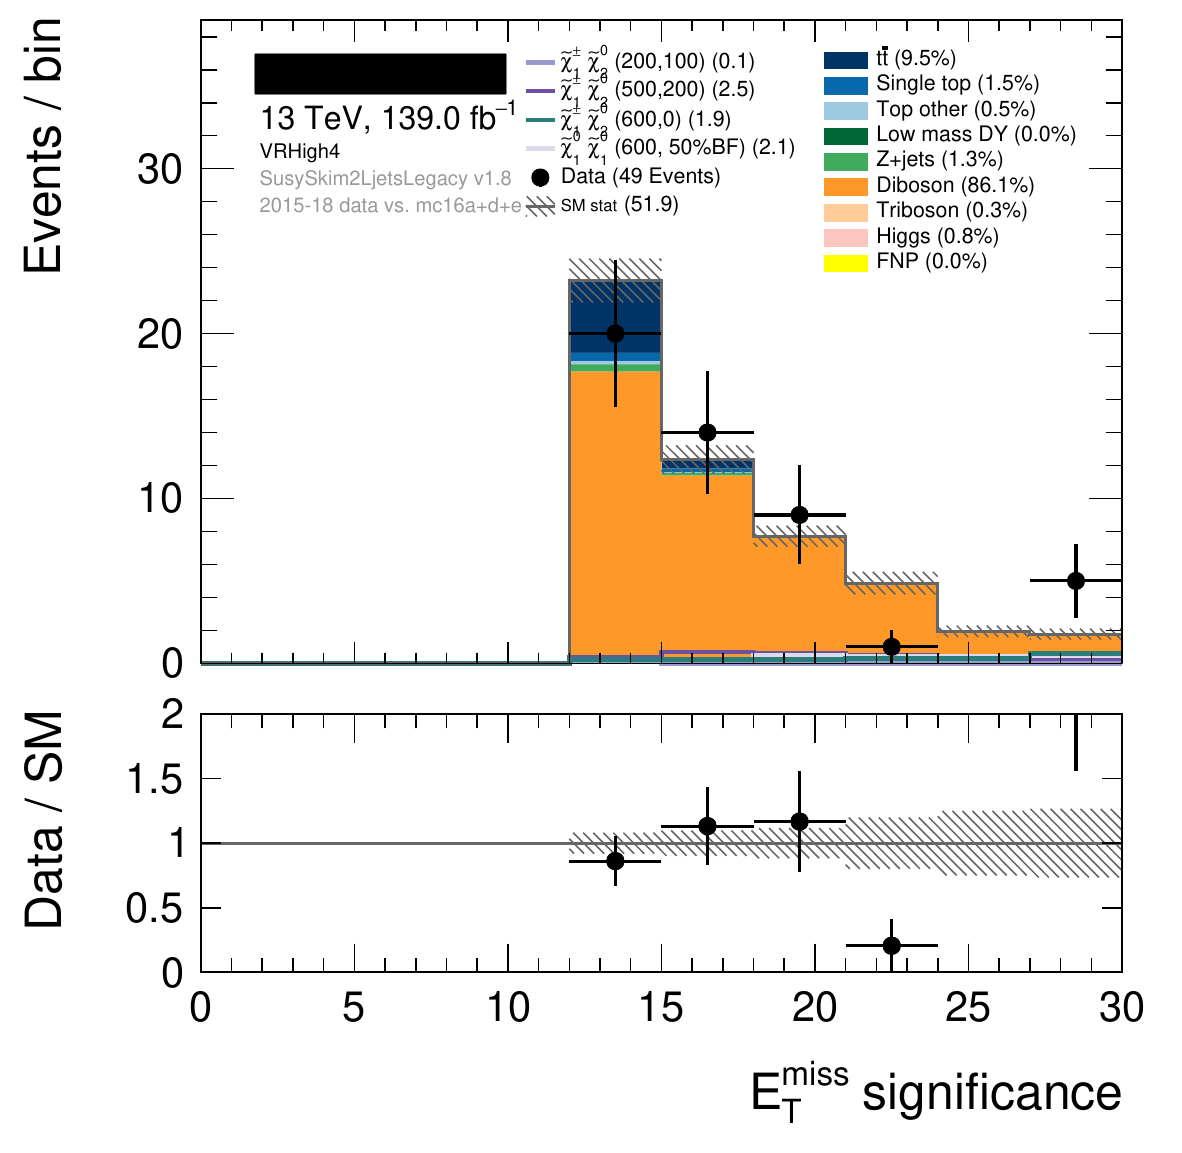
\includegraphics[width=\textwidth]{figures/2ljets_def_met_Sign_VRHigh4.png}
\caption{VR-High-1J, $\metsig$}
\end{subfigure}
\hfill
\begin{subfigure}{0.48\textwidth}
\centering
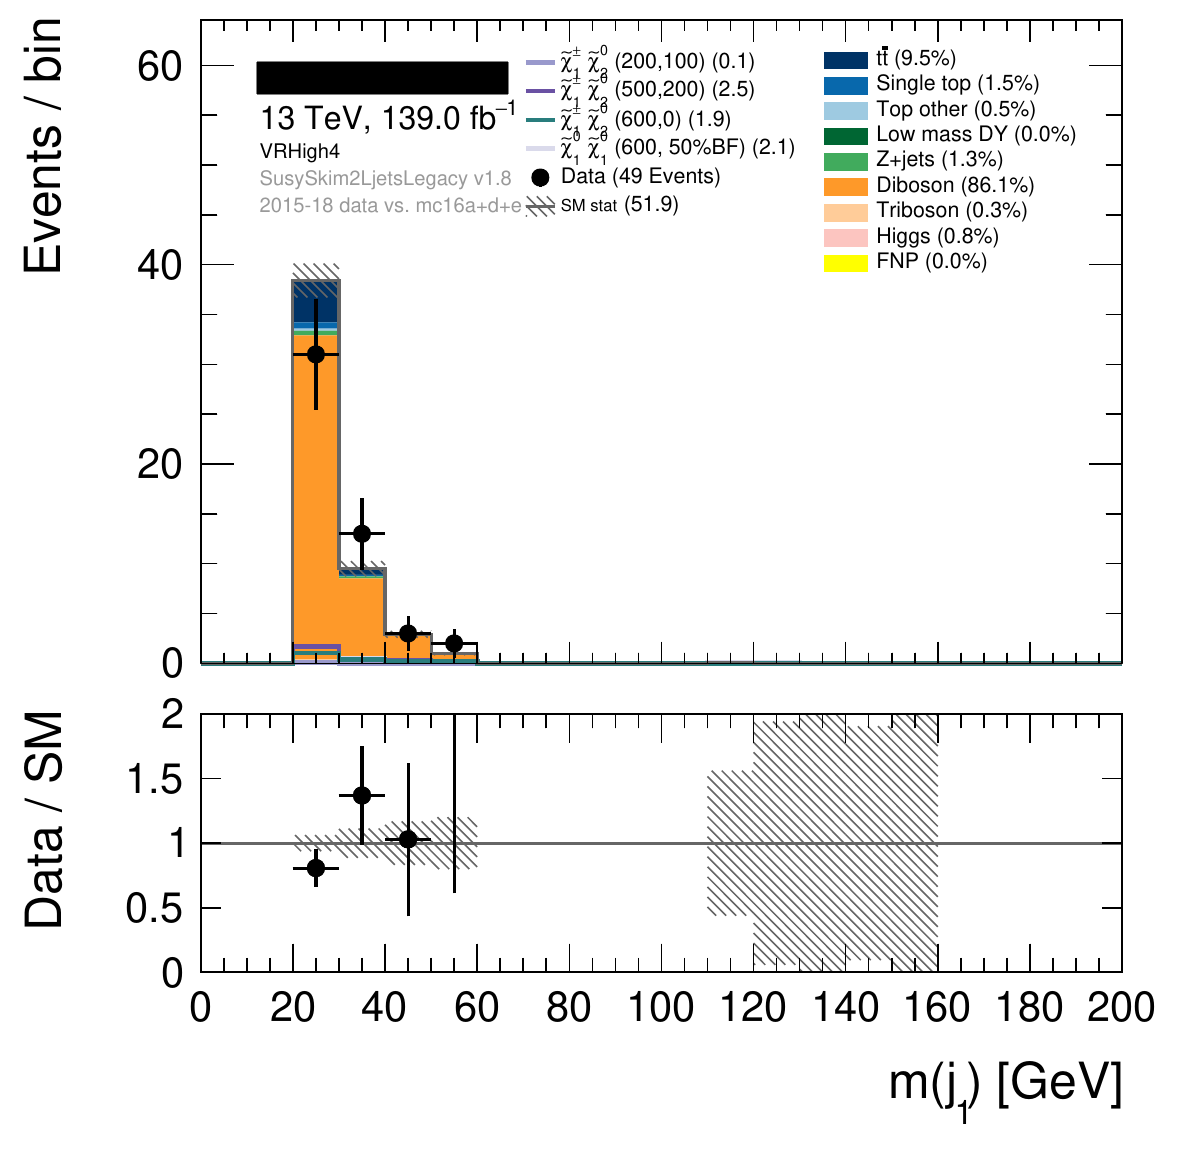
\includegraphics[width=\textwidth]{figures/2ljets_def_mjetone_VRHigh4.png}
\caption{SR-High-1J, $\mjetone$}
\end{subfigure}
\caption[
Pre-fit distributions in mono-jet signal and validation regions
]{%
Pre-fit distributions in mono-jet signal and validation regions.
Signal regions are unblinded.
Errors are statistical.
}
\label{fig:2ljets_high_1J_region}
\end{figure}

All other regions require two jets or more, so this single-jet selection has
the liberty to reduce its $\metsig$ requirement to $\metsig > 12$
without overlapping any other regions.

Finally, \srllbb\ is designed to target the GMSB model, which produces decays
via $ZZ$ and $Zh$ bosons pairs.
Since the $h\rightarrow bb$ branching fraction is large, \srllbb\ finds
sensitivity by requiring a pair of $b$-tagged jets in a heavy mass window.
The low edge of this $\mbb \in 60\textrm{--}150\,\eV[G]$ window is chosen not
only to accommodate \atlas' noisy reconstruction of $b$-jets, but also to
capture $Z\rightarrow bb$ decays, which become significant signal models with
small $B(\neutralino_1 \rightarrow h \gravitino)$.

As shown in Figure~\ref{fig:2ljets_high_llbb_region}, backgrounds in \srllbb
contain a significant proportion of \topother\ quark processes;
studies presented in Section~\ref{sec:2ljets_validation} show that these are
mainly $t\bar t Z$.

\begin{figure}[tp]
\centering
\begin{subfigure}{0.48\textwidth}
\centering
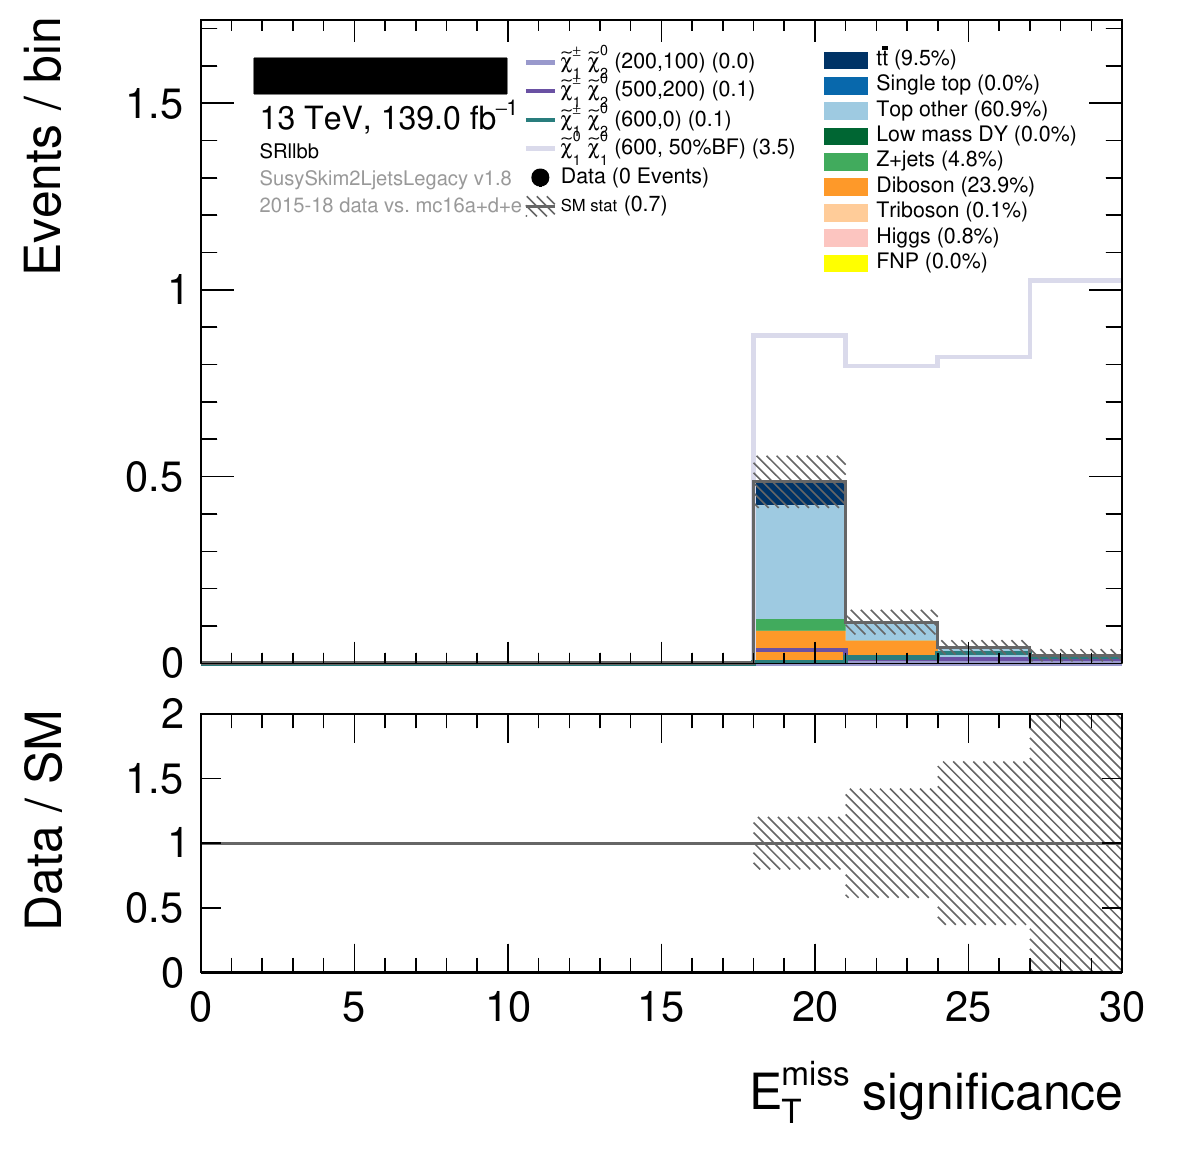
\includegraphics[width=\textwidth]{figures/2ljets_def_met_Sign_SRllbb.png}
\caption{\srllbb, $\metsig$}
\end{subfigure}
\hfill
\begin{subfigure}{0.48\textwidth}
\centering
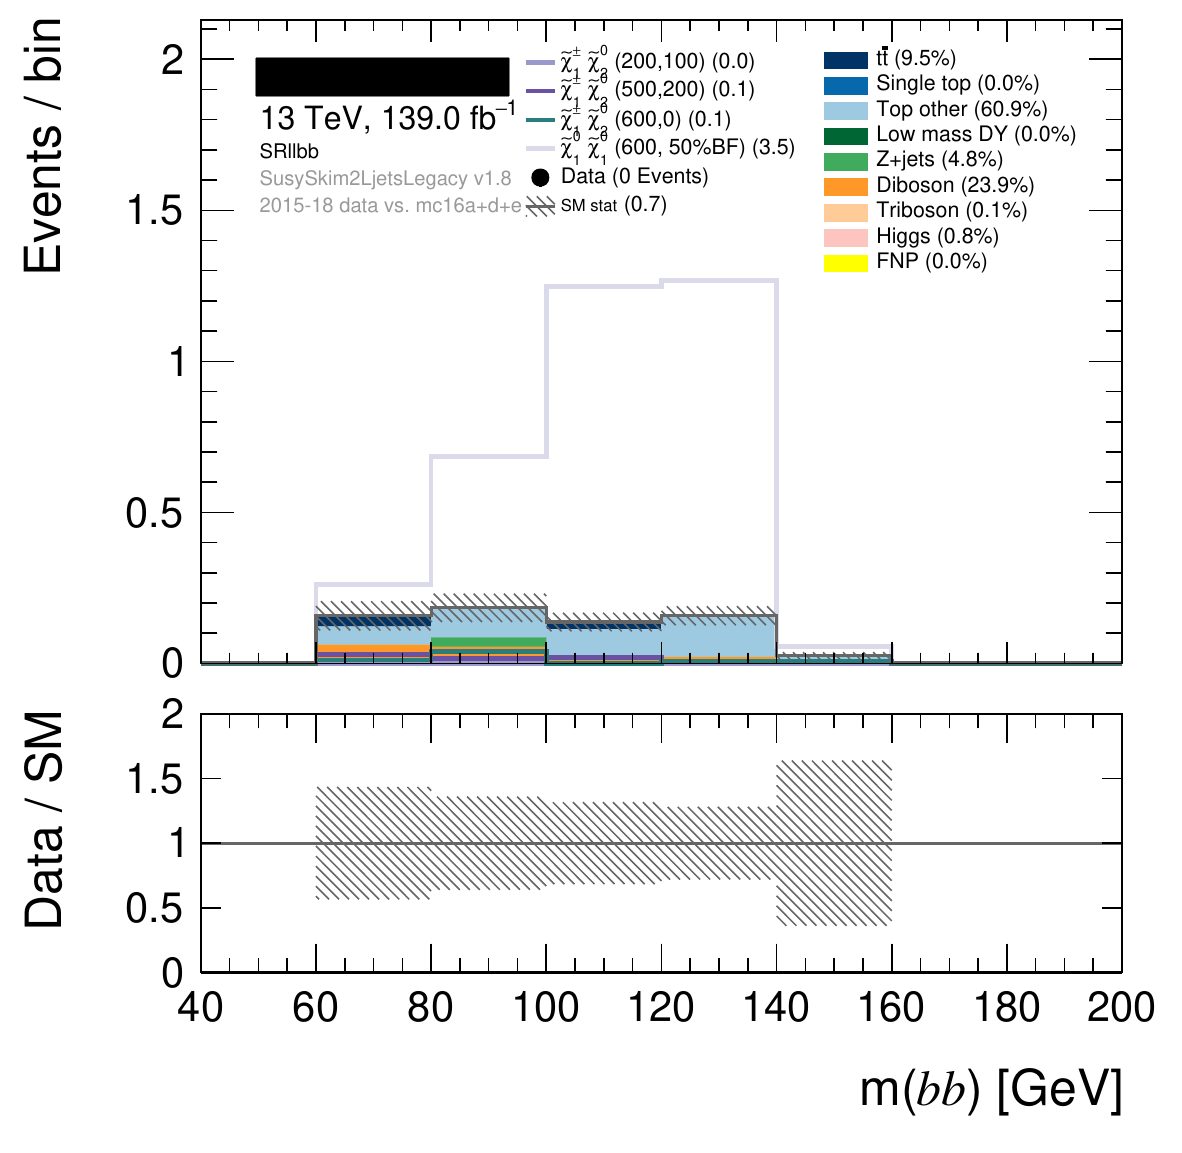
\includegraphics[width=\textwidth]{figures/2ljets_def_mbb_SRllbb.png}
\caption{\srllbb, $\mbb$}
\end{subfigure}
\\[0.5em]
\begin{subfigure}{0.48\textwidth}
\centering
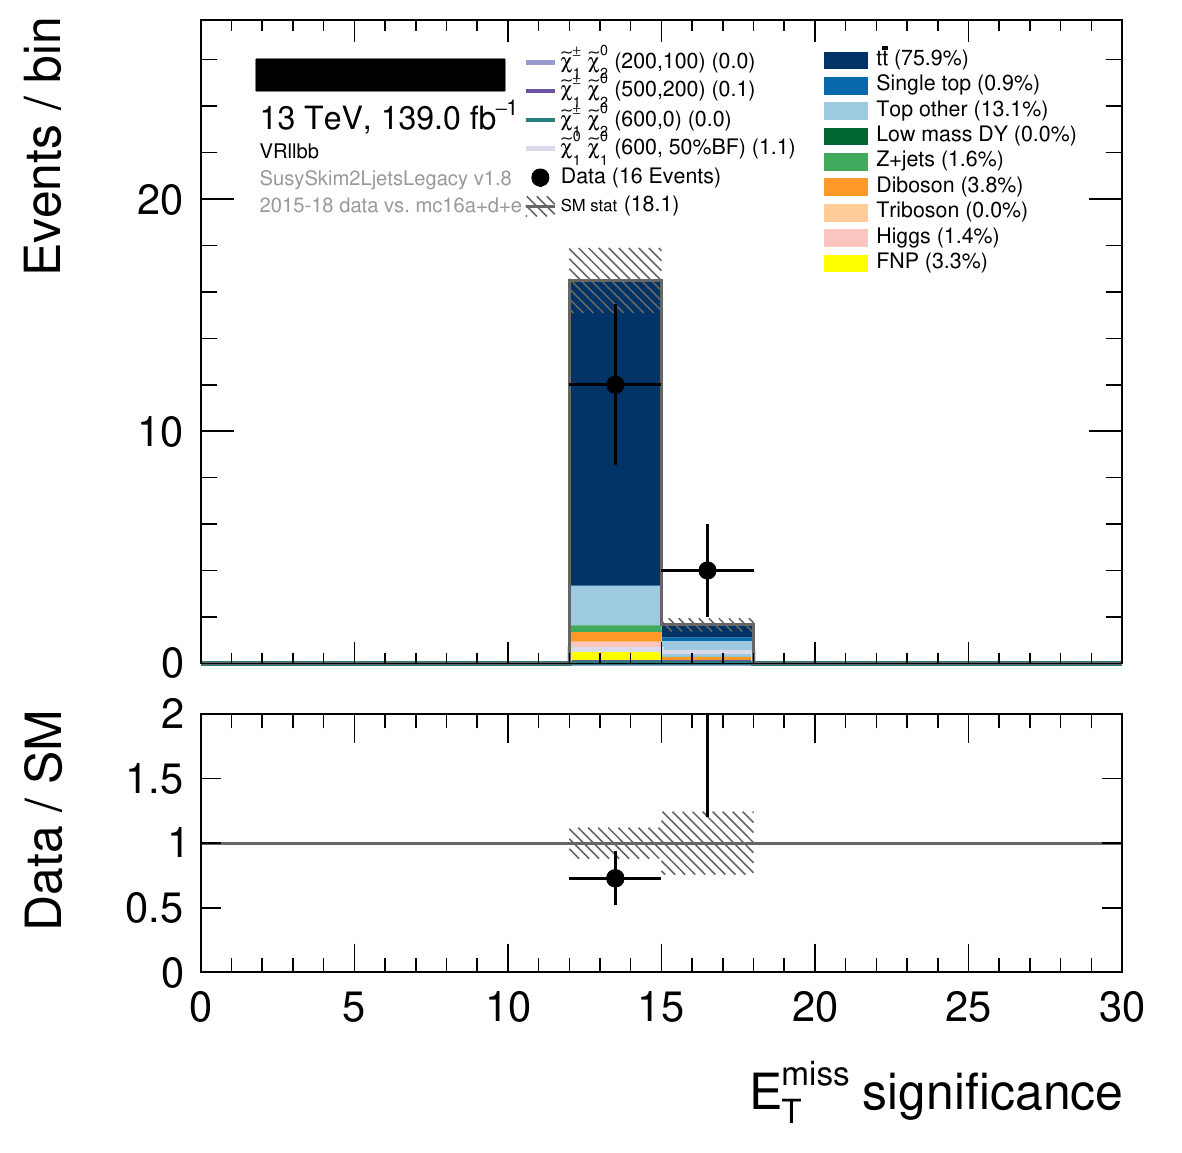
\includegraphics[width=\textwidth]{figures/2ljets_def_met_Sign_VRllbb.png}
\caption{VR-$\llbb$, $\metsig$}
\end{subfigure}
\hfill
\begin{subfigure}{0.48\textwidth}
\centering
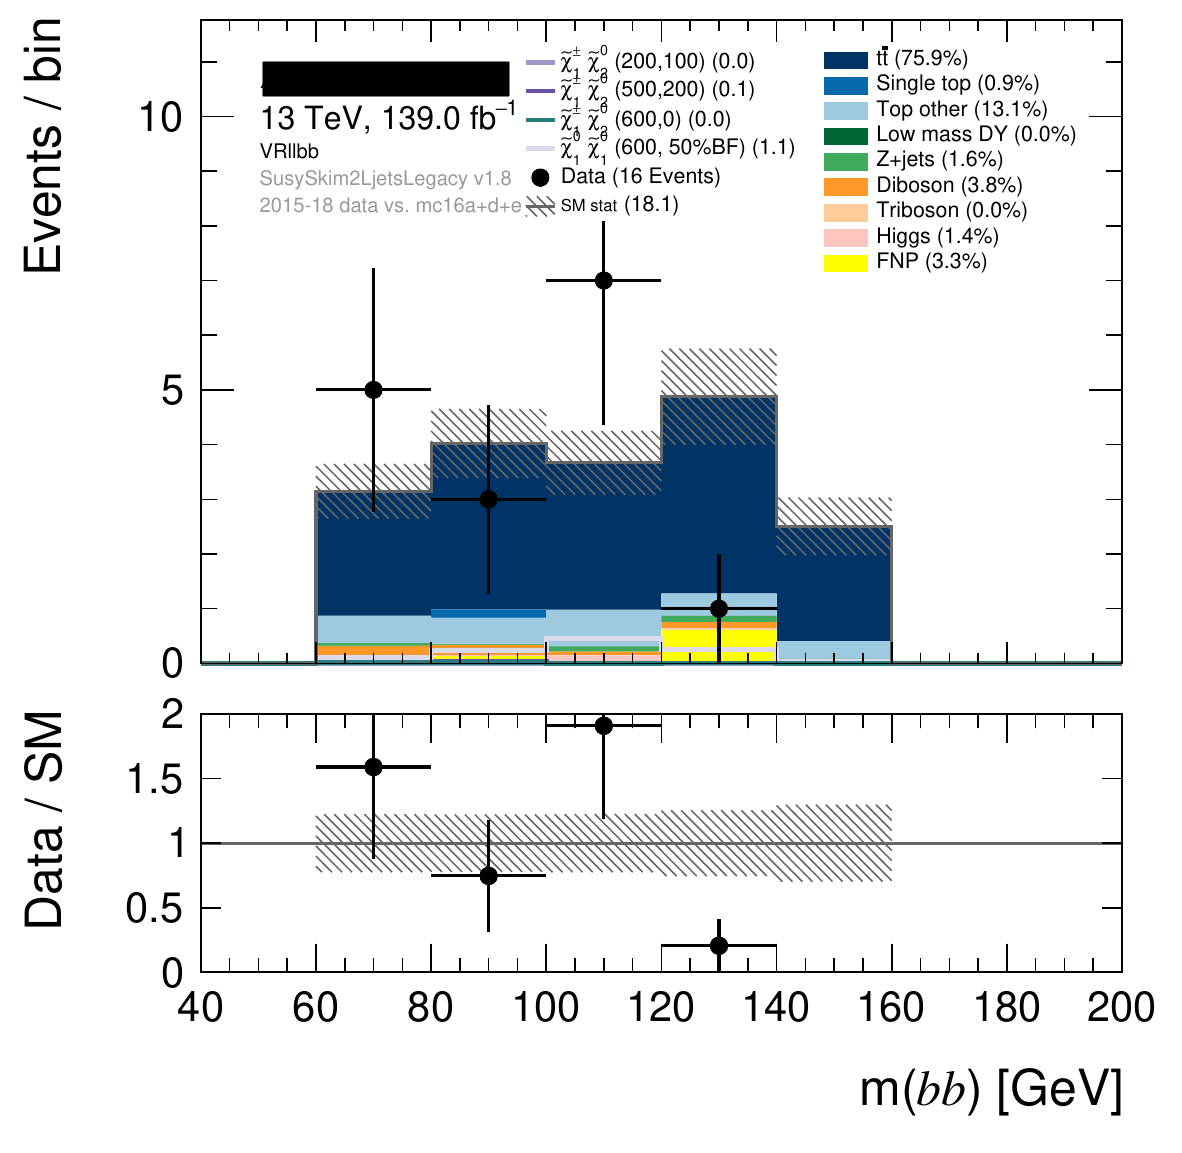
\includegraphics[width=\textwidth]{figures/2ljets_def_mbb_VRllbb.png}
\caption{VR-$\llbb$, $\mbb$}
\end{subfigure}
\caption[
Pre-fit distributions in $\llbb$ signal and validation regions
]{%
Pre-fit distributions in $\llbb$ signal and validation regions.
Signal regions are unblinded.
Errors are statistical.
}
\label{fig:2ljets_high_llbb_region}
\end{figure}

Validation regions, as always, are defined near to each signal region, under
the constraint of being somehow `nearby' and having enough data to test
background predictions.
For SR-High, inverting the selections on $\mjj$ or $\rjj$ satisfies
these criteria, so one validation region is designed on each.
An apparent excess appears at small $\mjj$ in VR-High, which is shown in
Figure~\ref{fig:2ljets_high_mjj_vrhigh}.

Various validation studies explored similar selections and different
simulated samples, and found no clear explanation for this effect.
It therefore motivates the second validation region VR-High-R, and is one
reason for including a lower bound of $\mjj > 20\,\eV[G]$ in all regions.
As seen in Figures~\ref{fig:2ljets_high_region}
and~\ref{fig:2ljets_high_mjj_vrhigh}, VR-High and VR-High-R otherwise show
acceptable pre-fit modelling even without systematic uncertainties.

\begin{figure}[tp]
\centering
\begin{subfigure}{0.48\textwidth}
\centering
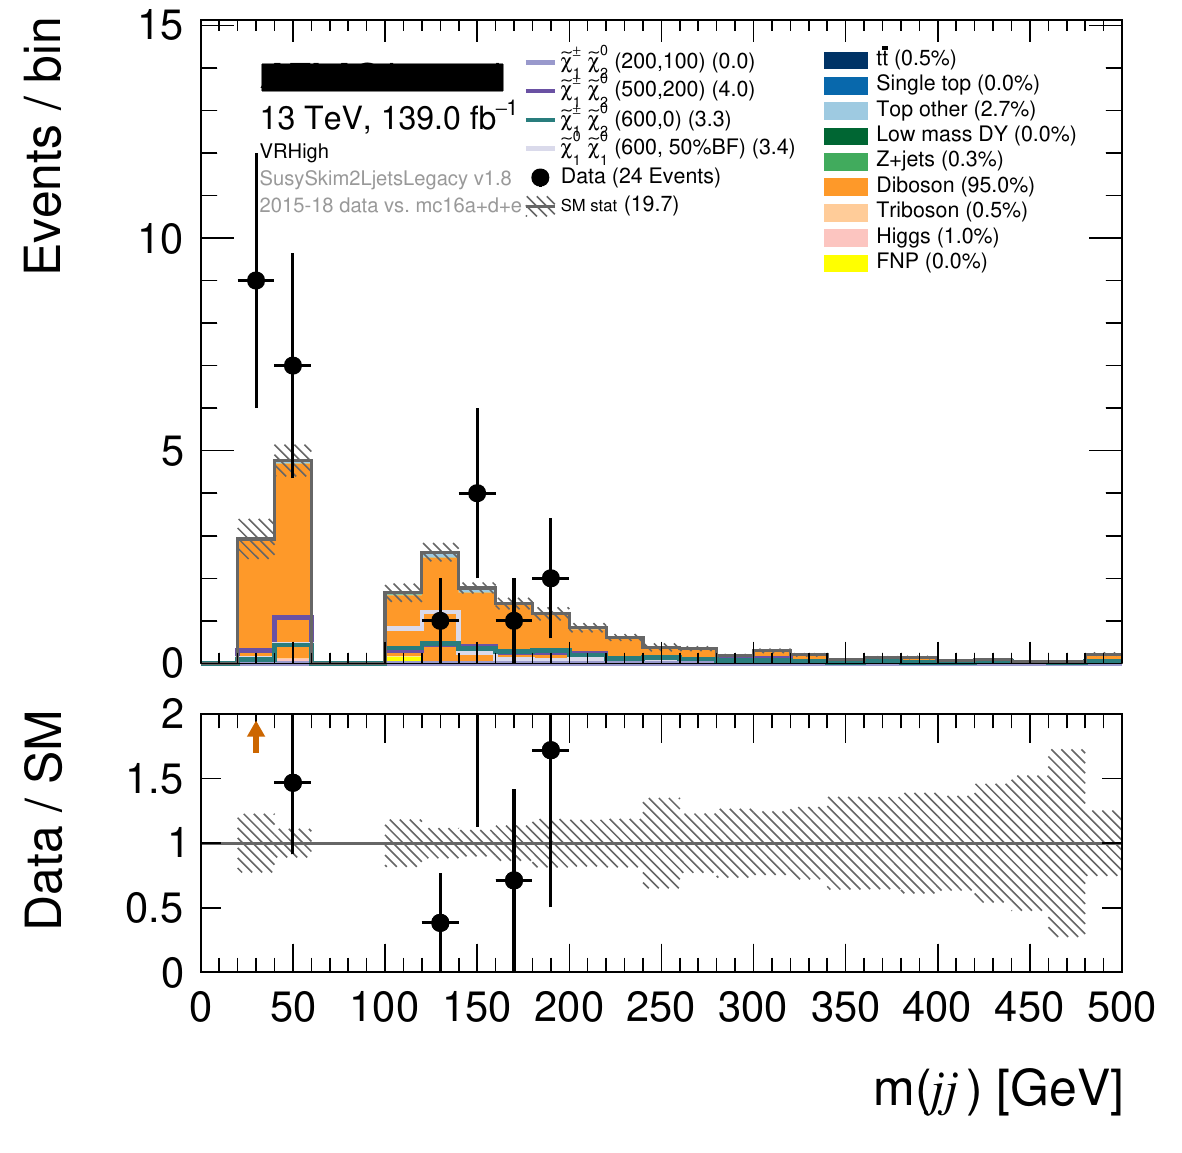
\includegraphics[width=\textwidth]{figures/2ljets_def_mjj_VRHigh.png}
\caption{VR-High, $\mjj$}
\end{subfigure}
\hfill
\begin{subfigure}{0.48\textwidth}
\centering
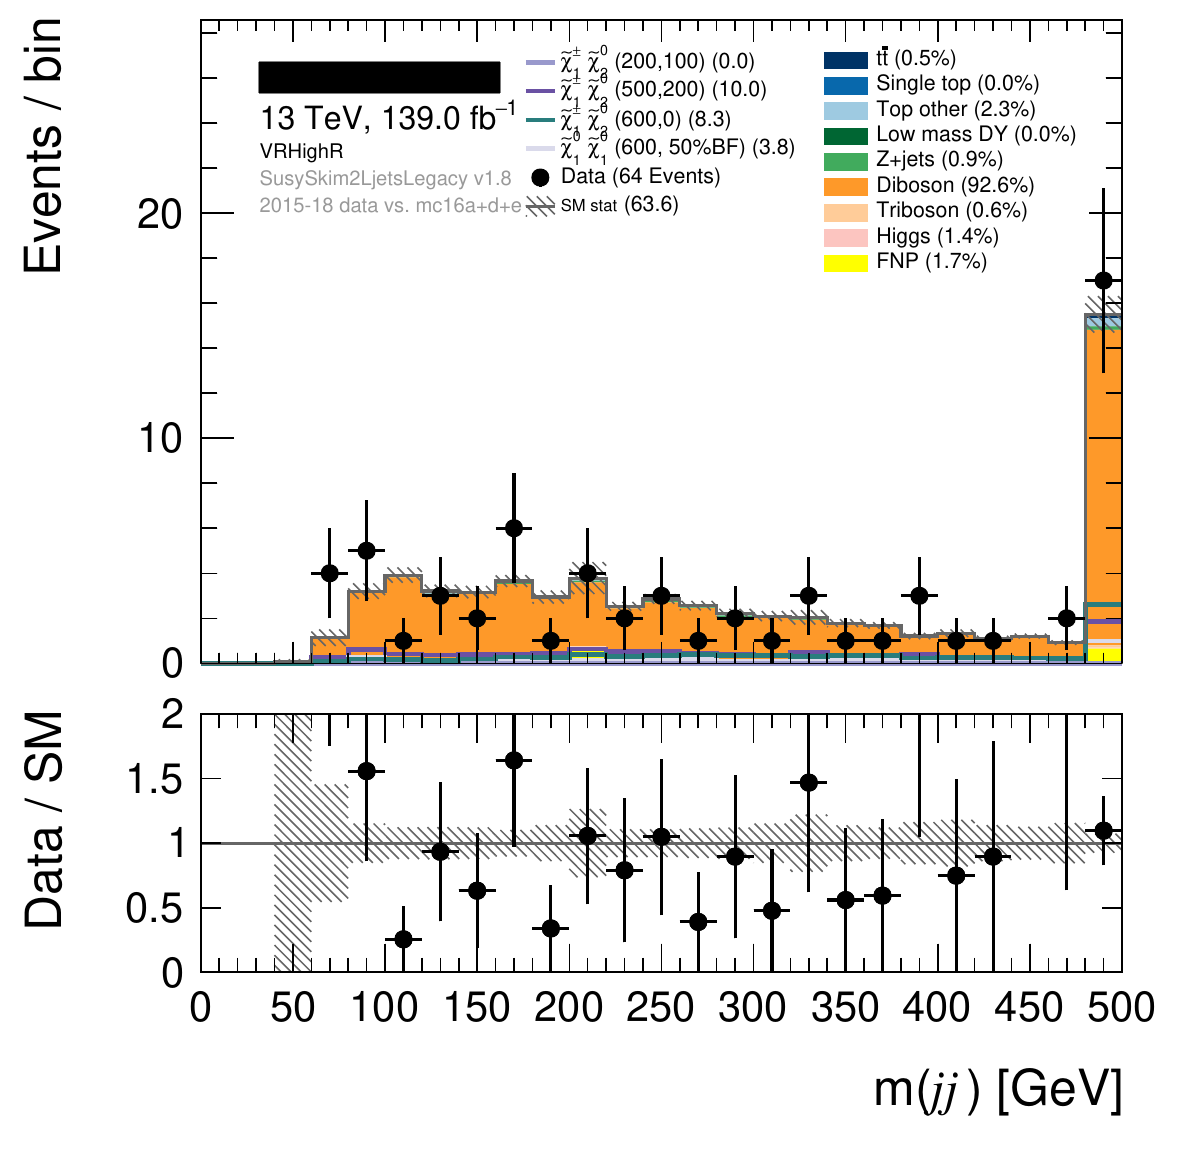
\includegraphics[width=\textwidth]{figures/2ljets_def_mjj_VRHighR.png}
\caption{VR-High-R, $\mjj$}
\end{subfigure}
\caption[
Pre-fit $\mjj$ distributions in validation regions VR-High and VR-High-R
]{%
Pre-fit $\mjj$ distributions in validation regions VR-High and VR-High-R.
Signal regions are unblinded.
Errors are statistical.
The apparent excess at low $\mjj$ in VR-High is not well understood.
}
\label{fig:2ljets_high_mjj_vrhigh}
\end{figure}

The distribution of mono-jet masses ($\mjetone$) is sharply peaked towards zero,
so cutting this out while inverting the $\mjetone$ selection of SR-High-1J
more clearly inspects the modelling of massive jets, which appears to be good.
Note that the region $\mjetone > 110$ is also checked in this validation region
and seen to contain no data.
This is good for the standard model.
Since background estimates are near zero up there, non-zero data would have
ruled out our modelling in favour of any model making small positive
predictions.

The small yields beside \srllbb\ in other event variables left $\metsig$ as
the only appropriate candidate to change for VR-$\llbb$.
Unfortunately, this region mostly checks $\ttbar$ backgrounds, and not the
rare $\ttbar Z$ backgrounds which we would most like to validate.
Early work observed good $\ttbar Z$ modelling in three- and four- lepton
selections, but these were excluded from the $\twoljets$ analysis for
orthogonality from other \atlas\ searches with which our results are to be
combined.

Total backgrounds predict data well in VR-$\llbb$.
What was not appreciated soon enough, however, was an excess in the $\metsig$
tail of this region, which is reproduced from the paper in
Figure~\ref{fig:2ljets_high_metsig_vrllbb_paper},
The highest bins have very small background predictions and positive data.
Had this been noticed before unblinding, more validation might have
been advisable.
``In the end'', comments one \atlas\ author,
``it seems fine since there's not events in the SR!''~\cite{comment2022vrllbb}.

\begin{figure}[tp]
\centering
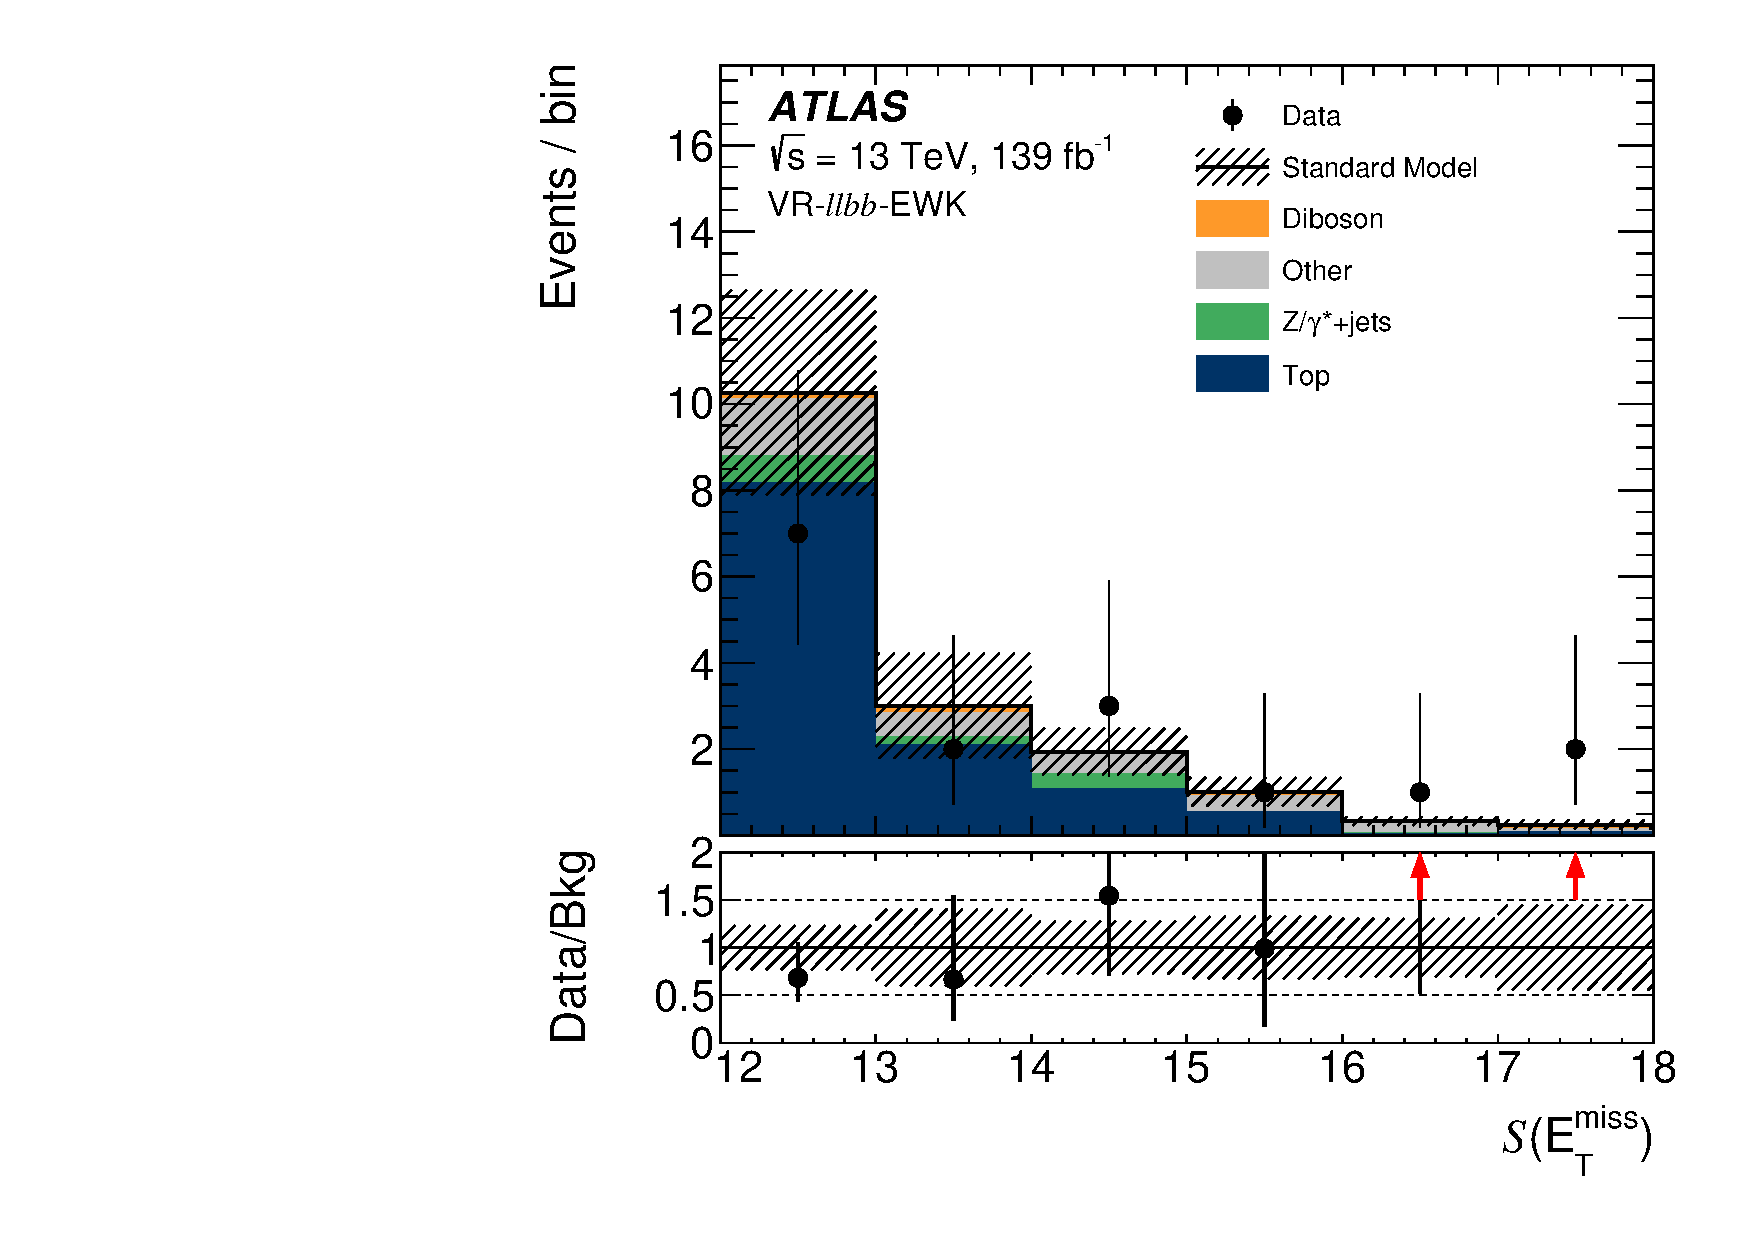
\includegraphics[width=0.48\textwidth]{figures/2ljets_vr_llbb_met_sig.pdf}
\caption[
Post-fit $\metsig$ distribution in VR-$\llbb$
]{%
Post-fit $\metsig$ distribution in VR-$\llbb$.
Backgrounds are to control and signal regions.
This region is also displayed pre-fit with coarser bins in
Figure~\ref{fig:2ljets_high_llbb_region}.
}
\label{fig:2ljets_high_metsig_vrllbb_paper}
\end{figure}


\FloatBarrier
\subsection{Intermediate}
\label{sec:2ljets_int}

Intermediate signal regions are defined to sit in the $\metsig$ range of
$12$ to $18$.
As seen from Figure~\ref{fig:2ljets_presel_met}, this space suffers from
$\ttbar$ background contributions, but it also receives substantial signal
yields from some lighter signal models.
The larger rates of background processes in this space also make it ripe for
control regions.

Intermediate signal regions are defined in Table~\ref{tab:2ljets_int},
along with their associated validation regions and the control regions in this
space.
To suppress the increased backgrounds, the intermediate $\mll$ window is
tightened to reduce non-$Z$ backgrounds, including $\ttbar$ and \diboson
processes.
Requiring zero $b$-tags further reduces $\ttbar$ backgrounds.

\begin{table}[tp]
\centering
\begin{tabular}{lccccc}
& $\njet$
& $\nbtag$
& $\metsig$
& $\mjj$
& $\ptjone$
\\[1em]
SR-Int
& $\geq 2$
& $\hphantom{\geq}~0$
& $12\textrm{--}15\textrm{--}18$
& $60\textrm{--}110$
& $> 60$
\\[0.5em]
\: VR-Int
& $\geq 2$
& $\hphantom{\geq}~0$
& $12\textrm{--}18$
& $60\textrm{--}110$
& $\uwave{< 60}$
\\[1em]
\crvz
& $\geq 2$
& $\hphantom{\geq}~0$
& $12\textrm{--}18$
& $\uwave{20\textrm{--}60 \mid 110\textrm{--}\infty}$
& $\uwave{\hphantom{< 60}}$
\\[0.5em]
\crtt
& $\geq 2$
& $\uwave{\geq 1}$
& $\uwave{9\textrm{--}12}$
& $\uwave{20}$
& $> 60$
\end{tabular}
\\[1em]
Common: Pre-selection,
$\njet \geq 2$,
$\mll \in 81\textrm{--}101$, and
$\mttwoll > 80$.
\caption[
Intermediate region definitions in the $\twoljets$-electroweak analysis
]{%
Intermediate region definitions in the $\twoljets$-electroweak analysis.
En-dashes `$a\textrm{--}b$' indicate open intervals $(a, b)$.
Concatenated intervals `$a\textrm{--}b\textrm{--}c$' indicate binning
with boundaries at $a$, $b$, and $c$.
The mid-bar `$\mid$' indicates logical or.
Differences between regions are \uwave{underlined}.
}
\label{tab:2ljets_int}
\end{table}

The less extreme signal models targeted here have less boosted
$W\rightarrow jj$ distributions, and so it was found that a $\ptjone$ selection
was effective at separating signals;
a $\ptjone > 60\,\eV[G]$ requirement split SR-Int from its validation region,
VR-Int and is seen from Figure~\ref{fig:2ljets_int_region} to retain most
signal contributions.
Following our standard pattern set with other signal regions, SR-Int is binned
in $\metsig$ in intervals of $3$ units to improve signal sensitivity.

\begin{figure}[tp]
\centering
\begin{subfigure}{0.48\textwidth}
\centering
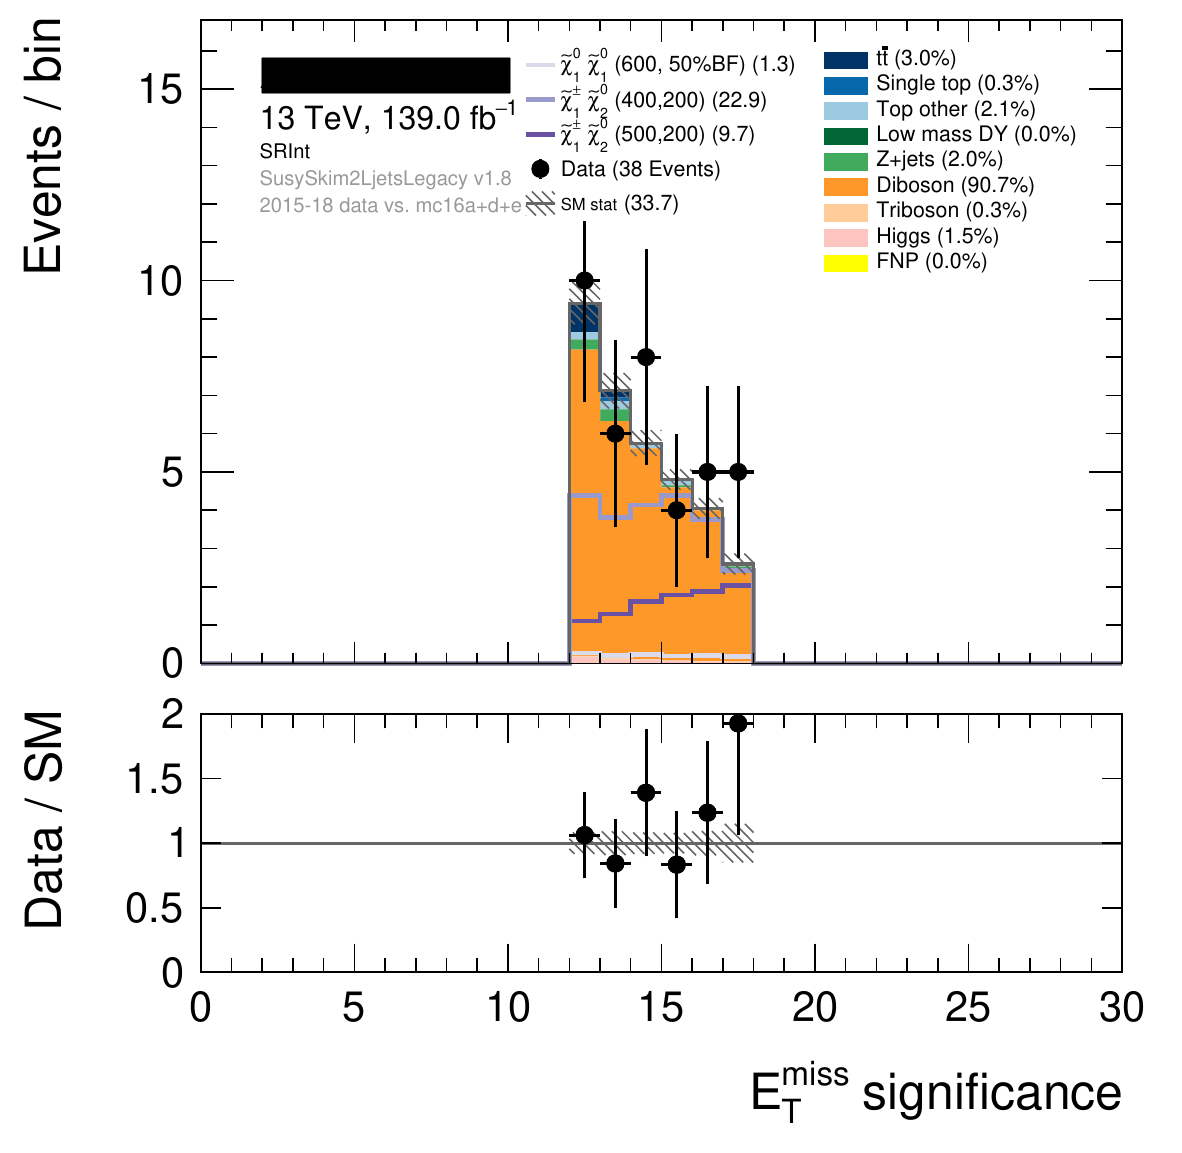
\includegraphics[width=\textwidth]{figures/2ljets_def_met_Sign_SRInt.png}
\caption{SR-Int, $\metsig$}
\end{subfigure}
\hfill
\begin{subfigure}{0.48\textwidth}
\centering
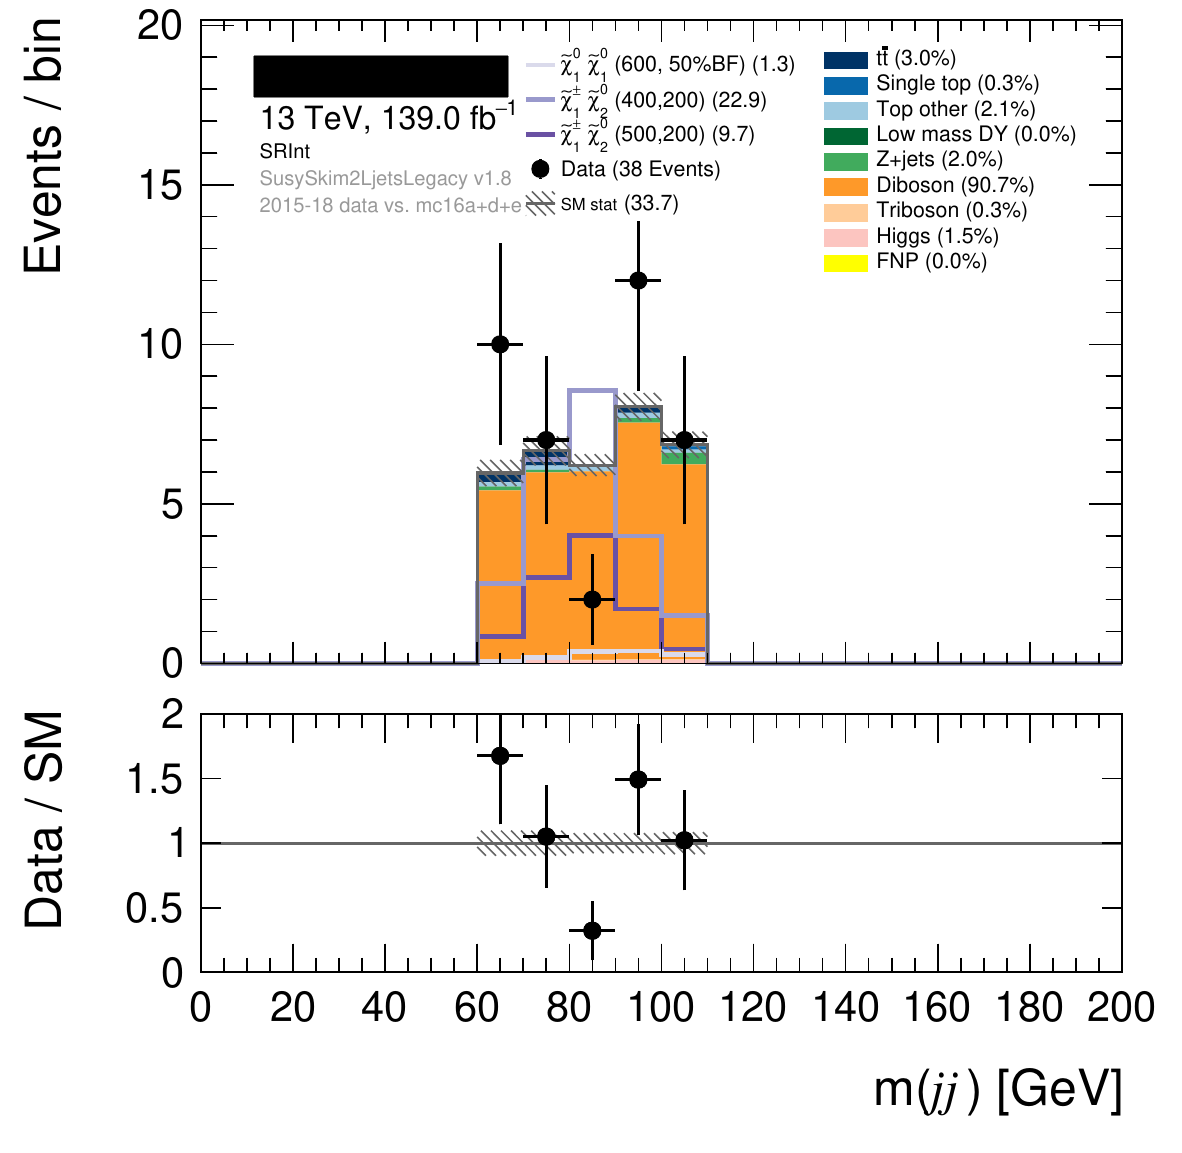
\includegraphics[width=\textwidth]{figures/2ljets_def_mjj_SRInt.png}
\caption{SR-Int, $\mjj$}
\end{subfigure}
\\[0.5em]
\begin{subfigure}{0.48\textwidth}
\centering
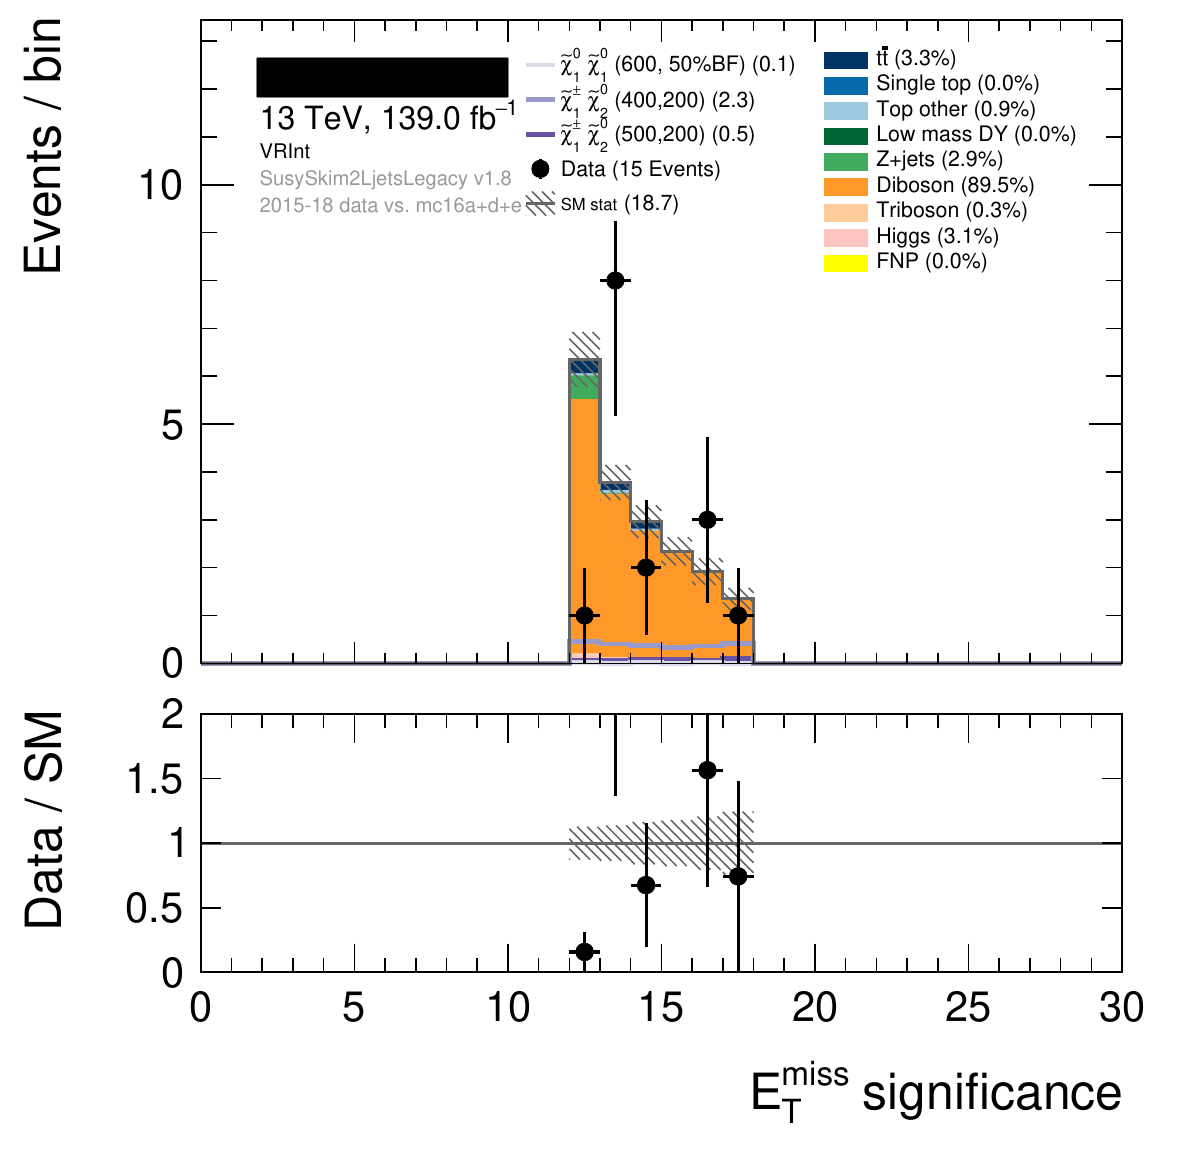
\includegraphics[width=\textwidth]{figures/2ljets_def_met_Sign_VRInt.png}
\caption{VR-Int, $\metsig$}
\end{subfigure}
\hfill
\begin{subfigure}{0.48\textwidth}
\centering
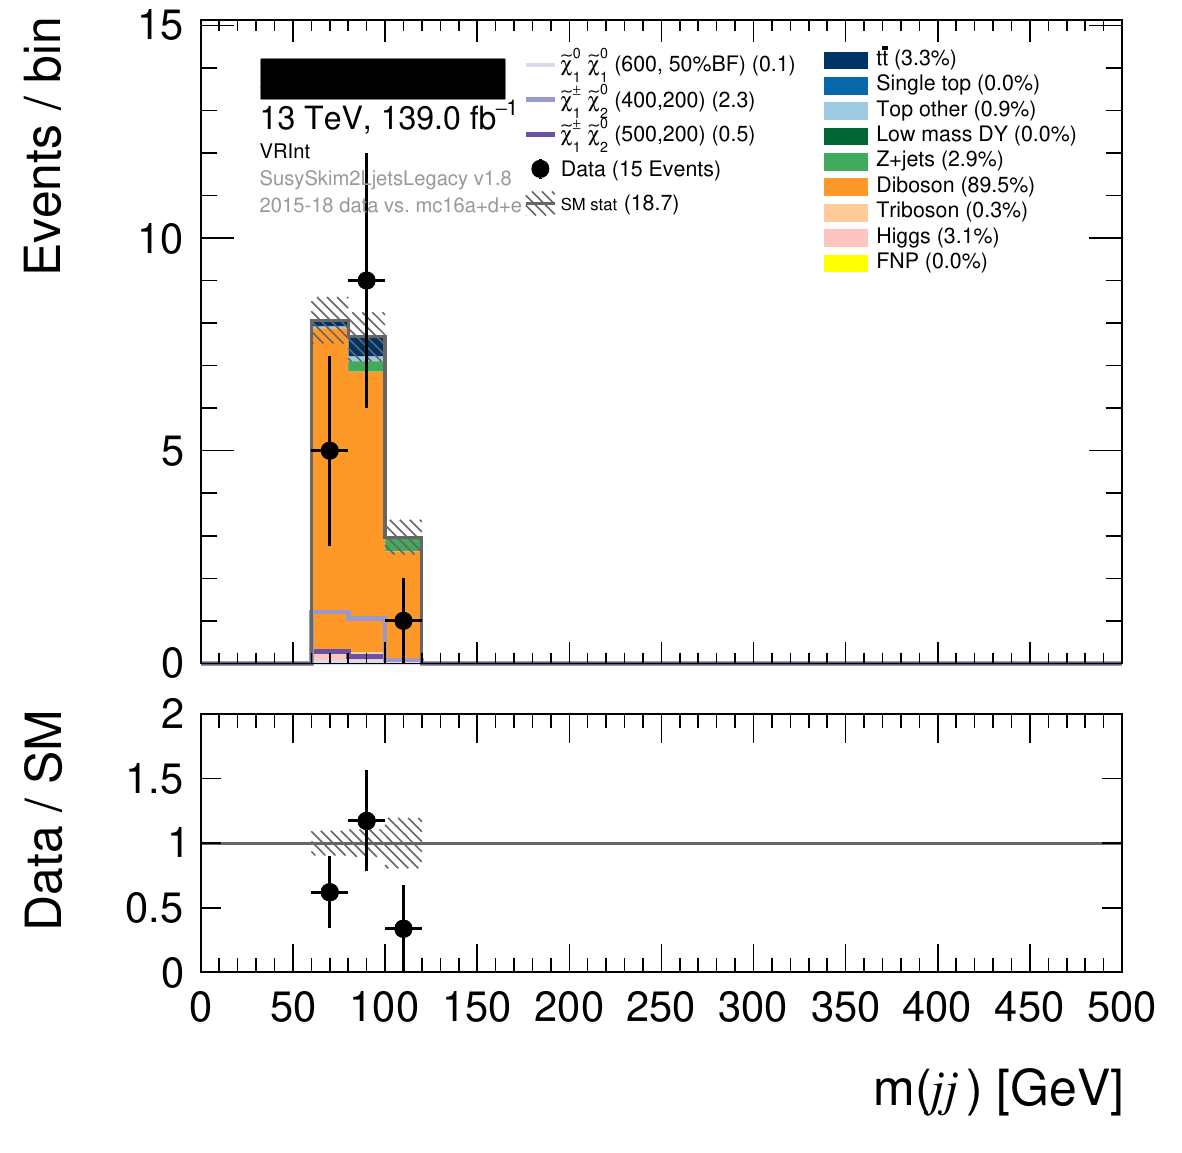
\includegraphics[width=\textwidth]{figures/2ljets_def_mjj_VRInt.png}
\caption{VR-Int, $\mjj$}
\end{subfigure}
\caption[
Pre-fit distributions in Intermediate signal and validation regions
]{%
Pre-fit distributions in Intermediate signal and validation regions.
Signal regions are unblinded.
Errors are statistical.
}
\label{fig:2ljets_int_region}
\end{figure}

The control region \crvz\ occupies the $\mjj$ side-band to
SR-Int and VR-Int.
As seen from Figure~\ref{fig:2ljets_int_cr_region}, the selections in this
intermediate space give \crvz\ a very pure \diboson\ background, which is very
valuable or constraining the modelling of High regions.
Also included in Table~\ref{tab:2ljets_int} and
Figure~\ref{fig:2ljets_int_cr_region} is \crtt, which uses various other
selections of $b$-tagged data to constrain $\ttbar$ backgrounds.
Both control regions show good agreement pre-fit and with statistical uncertainties
only.
\begin{figure}[tp]
\centering
\begin{subfigure}{0.48\textwidth}
\centering
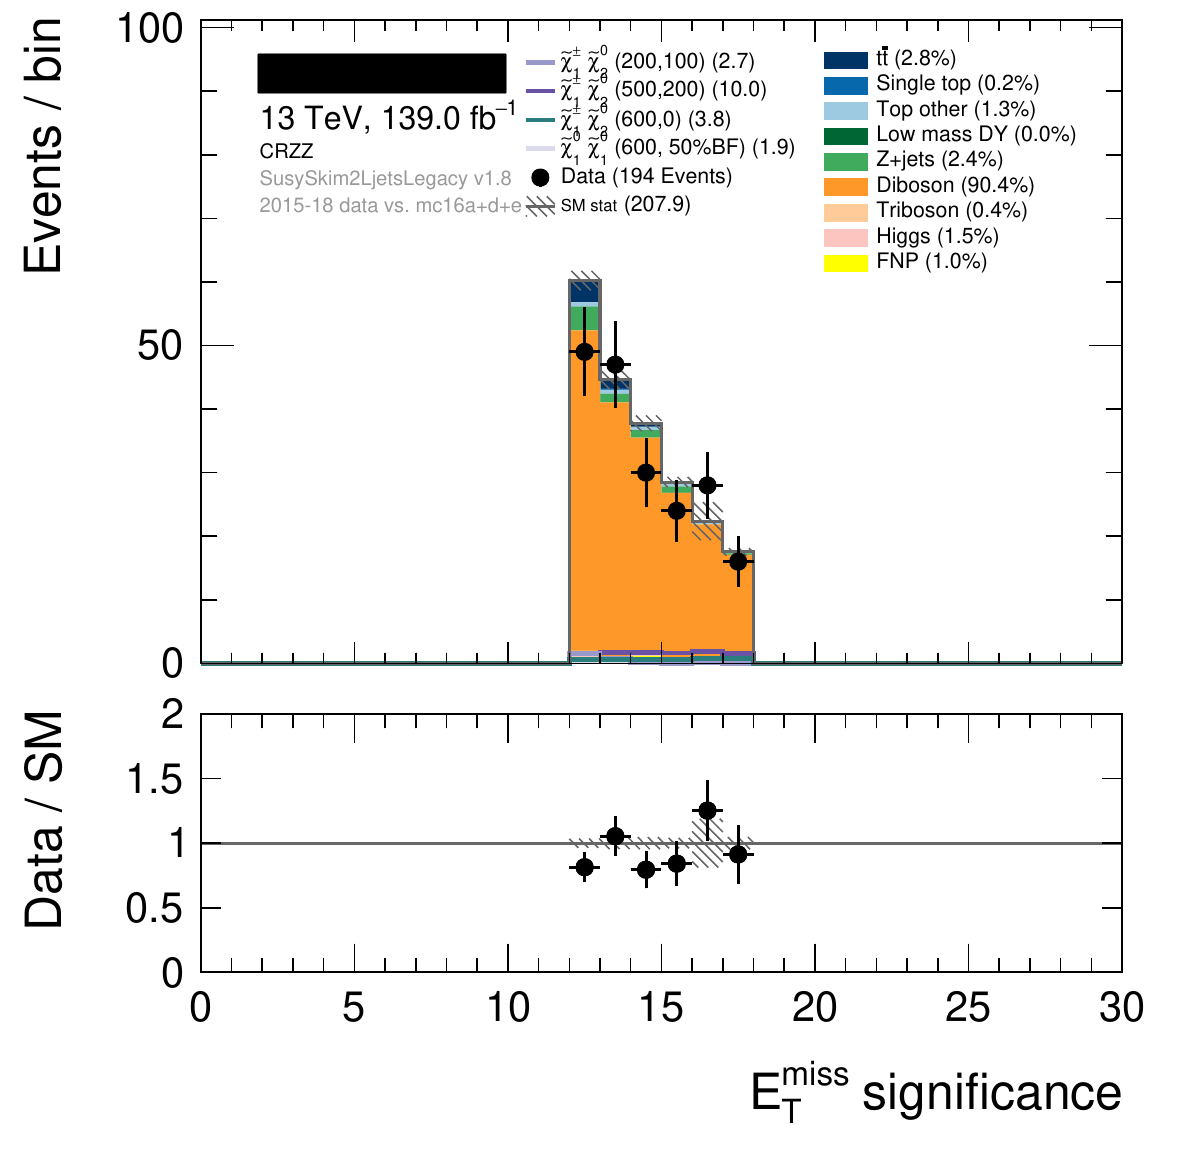
\includegraphics[width=\textwidth]{figures/2ljets_def_met_Sign_CRZZ.png}
\caption{\crvz, $\metsig$}
\end{subfigure}
\hfill
\begin{subfigure}{0.48\textwidth}
\centering
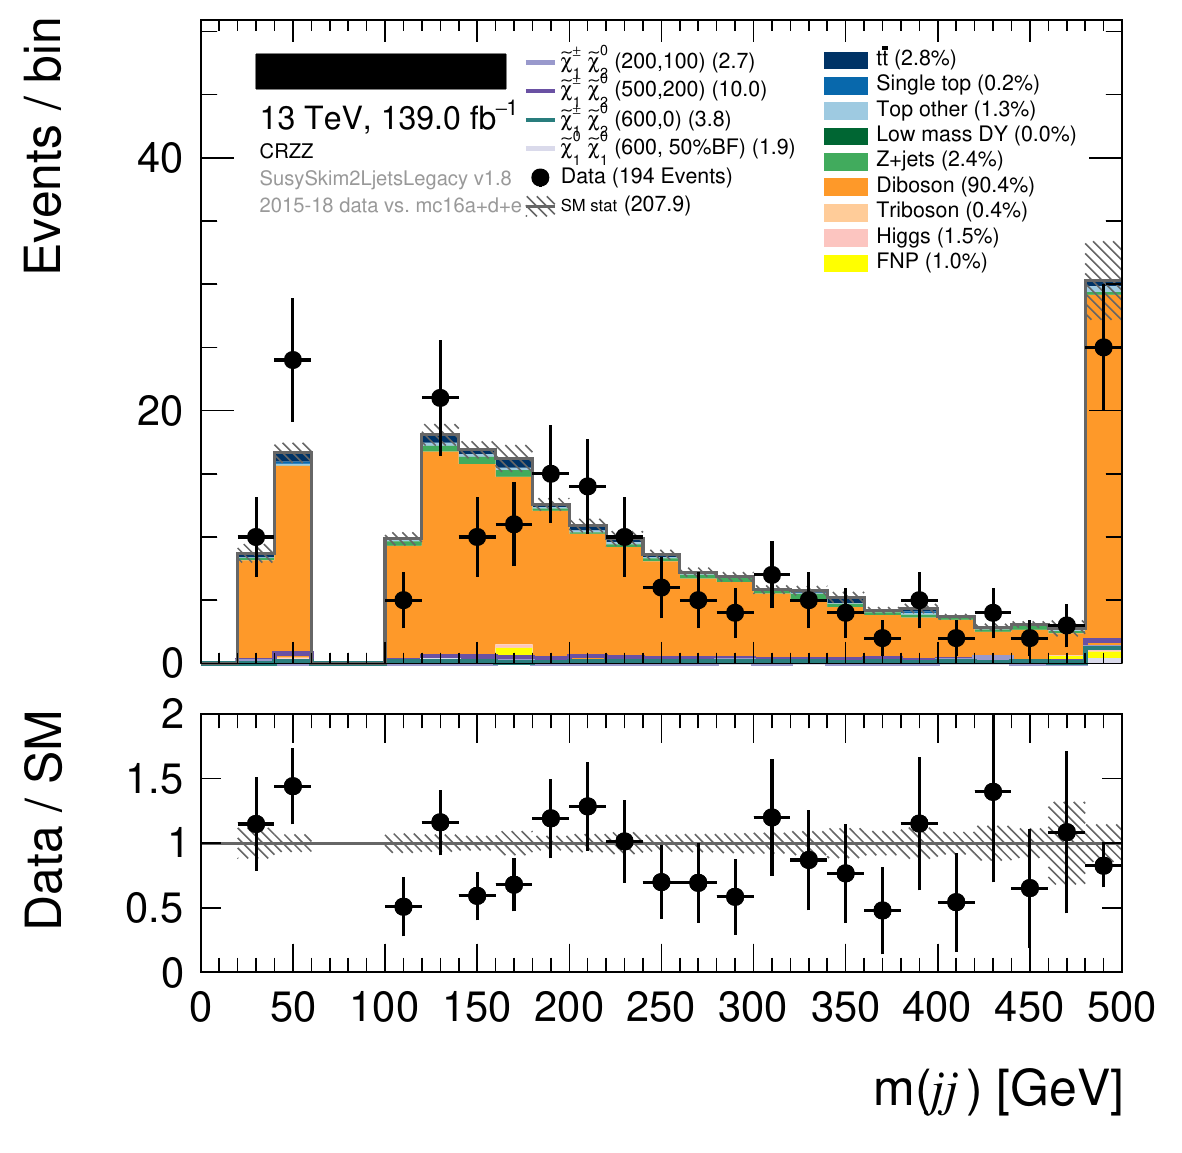
\includegraphics[width=\textwidth]{figures/2ljets_def_mjj_CRZZ.png}
\caption{\crvz, $\mjj$}
\end{subfigure}
\\[0.5em]
\begin{subfigure}{0.48\textwidth}
\centering
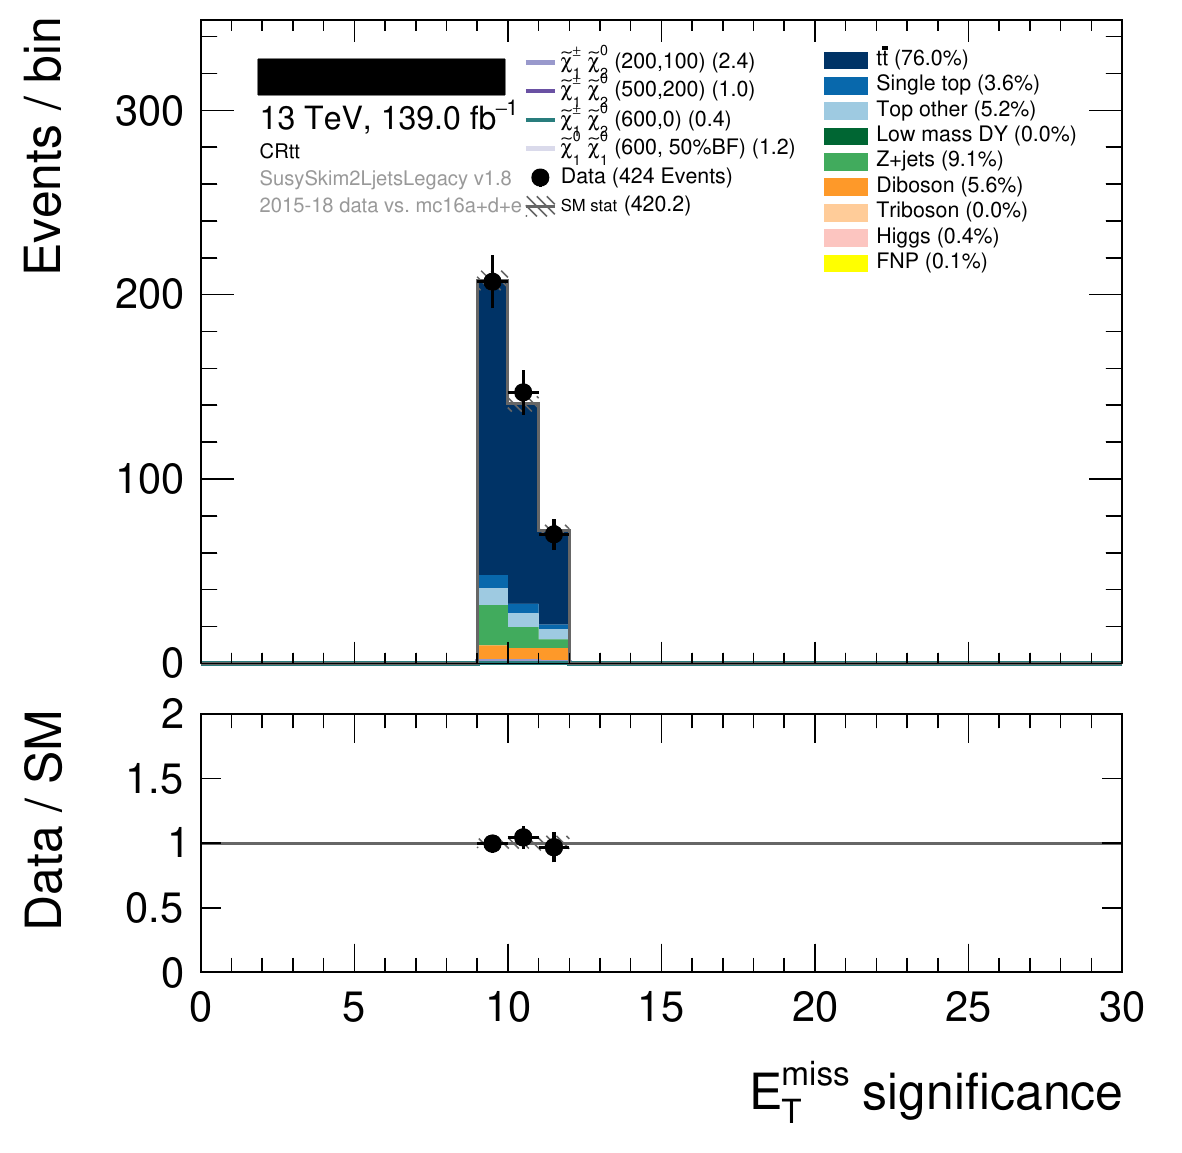
\includegraphics[width=\textwidth]{figures/2ljets_def_met_Sign_CRtt.png}
\caption{\crtt, $\metsig$}
\end{subfigure}
\hfill
\begin{subfigure}{0.48\textwidth}
\centering
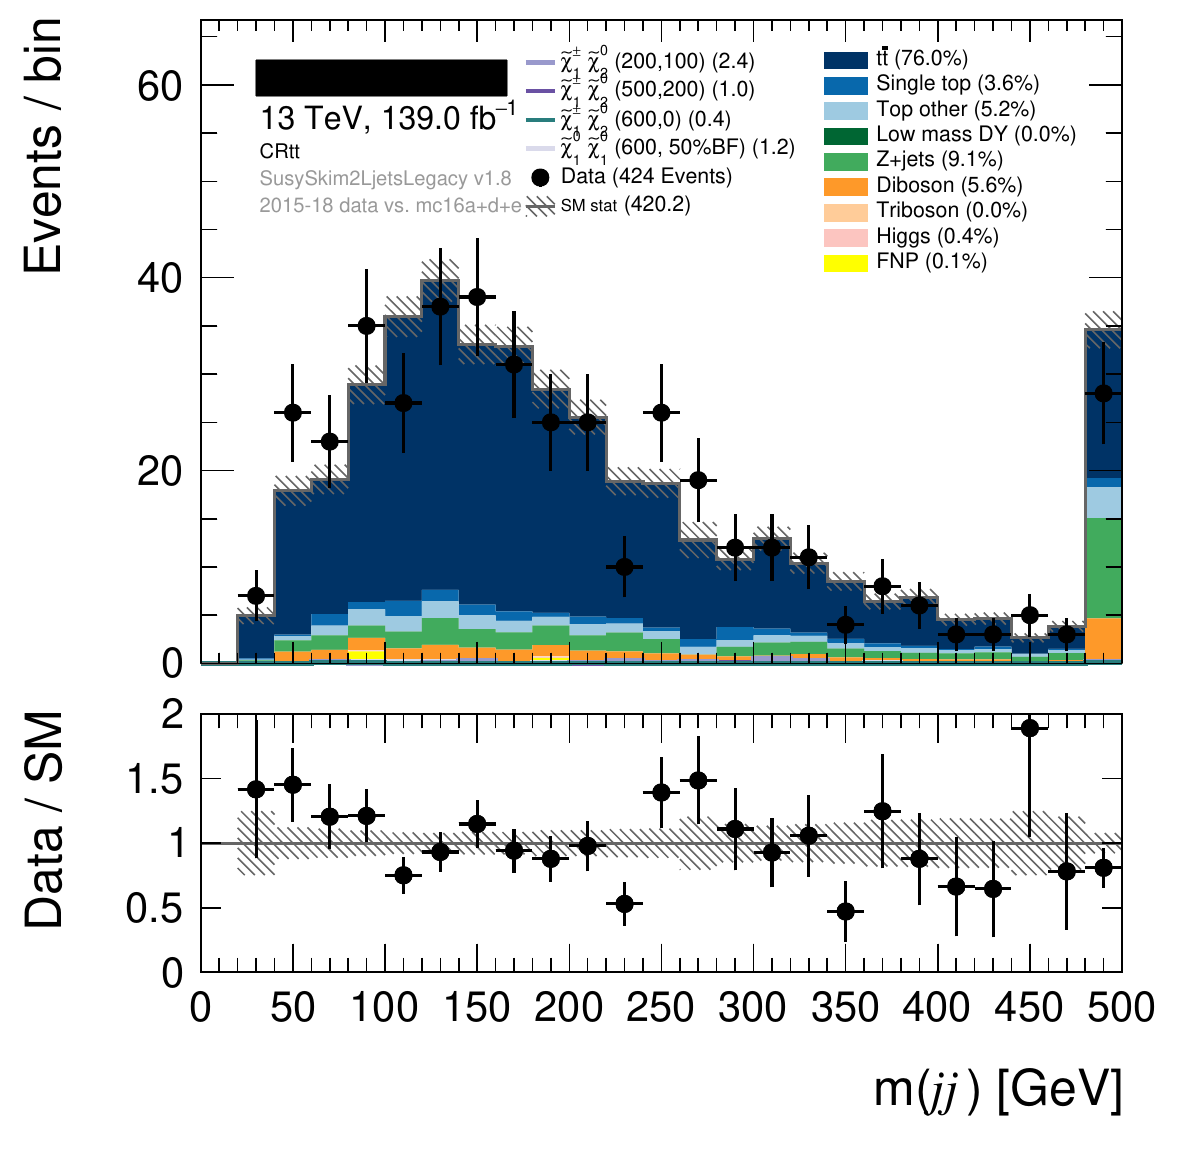
\includegraphics[width=\textwidth]{figures/2ljets_def_mjj_CRtt.png}
\caption{\crtt, $\mjj$}
\end{subfigure}
\caption[
Pre-fit distributions in the control regions CR-tt and CR-VZ
]{%
Pre-fit distributions in the control regions \crtt\ and \crvz.
Errors are statistical.
}
\label{fig:2ljets_int_cr_region}
\end{figure}

Some figures label \crvz\ as `\crz Z'; the region was renamed late in this
analysis project when it was show to contain substantial fractions of $W\kern-0.4exZ$
as well as $ZZ$, as illustrated in Figure~\ref{fig:2ljets_splits} of
Section~\ref{sec:2ljets_validation}.


\FloatBarrier
\subsection{Low}
\label{sec:2ljets_low}
In Low regions, which have $\metsig \in 6\textrm{--}12$, the $\zjets$
background becomes a large since its fake $\met$, which arises from
from mismeasurements or rare interactions, is no longer eliminated.
Similarly, backgrounds from $\ttbar$ increase; the selections inherited from
Intermediate regions to suppress $\ttbar$ need supplementing.

These regions target signal models with small mass splittings which still
exceed the masses of electroweak bosons.
In particular, we aim to test C1N2($200$, $100$) as a light, on-shell
benchmark which has not previously been excluded in this channel.

Angular selections on lepton variables $\rll$ and $\dphillmet$ characterize
the Low regions, which are defined in Table~\ref{tab:2ljets_low}.
These angular variables usefully reject backgrounds including $\ttbar$, and
provide signal sensitivity to benchmark signal models, as illustrated in
Figure~\ref{fig:2ljets_low_minus};
signals with small mass-splittings of around $100\textrm{--}150\,\eV[G]$
are targetted.

To remove some observed mis-modelling of backgrounds, Low regions require
exactly two jets.
Abandoned region designs which used more jets are discussed below in
Section~\ref{sec:2ljets_low_isr}.

\begin{table}[tp]
\centering
\begin{tabular}{lcccccccc}
& $\metsig$
& $\mjj$
& $\mttwoll$
& $\rll$
& $\dphillmet$
\\[1em]
SR-Low
& $6\textrm{--}9\textrm{--}12$
& $60\textrm{--}110$
& $> 80$
& $< 1$
&
\\[0.5em]
\: VR-Low
& $6\textrm{--}12$
& $60\textrm{--}110$
& $>80$
& $\uwave{1\textrm{--}1.4}$
&
\\[1em]
SR-Low-2
& $6\textrm{--}9$
& $60\textrm{--}110$
& $< 80$
& $< 1.6$
& $< 0.6$
\\[0.5em]
\: VR-Low-2
& $6\textrm{--}9$
& $\uwave{20\textrm{--}60 \mid 110\textrm{--}\infty}$
& $< 80$
& $< 1.6$
& $< 0.6$
\\[1em]
\crz
& $6\textrm{--}9$
& $\uwave{20\textrm{--}60 \mid 110\textrm{--}\infty}$
& $> 80$
& $\uwave{\hphantom{< 1.6}}$
& $\uwave{\hphantom{< 0.6}}$
\end{tabular}
\\[1em]
Common: Pre-selection,
$\njet = 2$,
$\nbtag = 0$, and
$\mll \in 81\textrm{--}101$.
\caption[
Low region definitions in the $\twoljets$-electroweak analysis
]{%
Low region definitions in the $\twoljets$-electroweak analysis.
En-dashes `$a\textrm{--}b$' indicate open intervals $(a, b)$.
Concatenated intervals `$a\textrm{--}b\textrm{--}c$' indicate binning
with boundaries at $a$, $b$, and $c$.
The mid-bar `$\mid$' indicates logical or.
Differences between regions are \uwave{underlined}.
}
\label{tab:2ljets_low}
\end{table}

Boosted $Z\rightarrow \ell^+\ell^-$ decays will tend to have small $\rll$.
Similarly to $\rjj$ in the High regions, this can usefully select signals,
but here also works to reject other $\ell^+\ell^-$ production mechanisms which
produce leptons is less correlated directions, particularly dileptonic
$\ttbar$.
As elsewhere, binning of SR-Low in $\metsig \in 6\textrm{--}9\textrm{--}12$
to form SR-Low-a and SR-Low-b respectively, increases sensitivity.

Unblinded, pre-fit histograms of SR-Low are shown in
Figure~\ref{fig:2ljets_low_region}.
Note that these plots do not include systematic uncertainties, so the meaning
of the observed data deficits cannot yet be fully interpreted.
This figure also includes VR-Low, which observes the high $\rll$ edge and
predicts the data well.

\begin{figure}[tp]
\centering
\begin{subfigure}{0.48\textwidth}
\centering
\includegraphics[width=\textwidth]{figures/2ljets_low_Rll_SRLow_noRll.pdf}
\caption{SR-Low$/\{\rll\}$}
\end{subfigure}
\hfill
\begin{subfigure}{0.48\textwidth}
\centering
\includegraphics[width=\textwidth]{figures/2ljets_low_mt2leplsp_0_SRLow_noRll_nomt2.pdf}
\caption{SR-Low$/\{\rll,\mttwoll\}$}
\label{fig:2ljets_low_minus_norll_nomt2_mt2}
\end{subfigure}
\\[0.5em]
\begin{subfigure}{0.48\textwidth}
\centering
\includegraphics[width=\textwidth]{figures/2ljets_low_absdPhiPllMet_SRLow2_noDphi.pdf}
\caption{SR-Low-2$/\{\dphillmet\}$}
\label{fig:2ljets_low_minus_dphi}
\end{subfigure}
\hfill
\begin{subfigure}{0.48\textwidth}
\centering
\includegraphics[width=\textwidth]{figures/2ljets_low_absdPhiPllMet_SRLow2_noDphi_mg5.pdf}
\caption{SR-Low-2$/\{\dphillmet\}$ (alt)}
\label{fig:2ljets_low_minus_dphi_alt}
\end{subfigure}
\caption[
Relaxed versions of SR-Low and SR-Low-2 to motivate their angular selections
]{%
Relaxed versions of SR-Low and SR-Low-2 to motivate their angular selections.
Each removes requirements listed in Table~\ref{tab:2ljets_low}:
(a) SR-Low removes $\rll$,
(b) SR-Low removes $\rll$ and $\mttwoll$,
and
(c, d) SR-Low-2 removes $\dphillmet$.
\\[0.5em]
Signals trend towards small $\rll$, plausibly due to their more boosted
$Z\rightarrow \ell^+\ell^-$ decays; small $\rll$ also suppresses $\ttbar$.
The mass of signals seen at small $\mttwoll$ in (b) motivates the design of
SR-Low-2.
Signals in SR-Low-2 spike at small $\dphillmet$ in (c); better statistical
precision is provided by an alternative $\zjets$ sample in (d).
}
\label{fig:2ljets_low_minus}
\end{figure}

\begin{figure}[tp]
\centering
\begin{subfigure}{0.48\textwidth}
\centering
\includegraphics[width=\textwidth]{figures/2ljets_def_met_Sign_SRLow.png}
\caption{SR-Low, $\metsig$}
\end{subfigure}
\hfill
\begin{subfigure}{0.48\textwidth}
\centering
\includegraphics[width=\textwidth]{figures/2ljets_def_mjj_SRLow.png}
\caption{SR-Low, $\mjj$}
\end{subfigure}
\\[0.5em]
\begin{subfigure}{0.48\textwidth}
\centering
\includegraphics[width=\textwidth]{figures/2ljets_def_met_Sign_VRLow.png}
\caption{VR-Low, $\metsig$}
\end{subfigure}
\hfill
\begin{subfigure}{0.48\textwidth}
\centering
\includegraphics[width=\textwidth]{figures/2ljets_def_mjj_VRLow.png}
\caption{VR-Low, $\mjj$}
\end{subfigure}
\caption[
Pre-fit distributions in Low signal and validation regions
]{%
Pre-fit distributions in Low signal and validation regions.
Signal regions are unblinded.
Errors are statistical.
}
\label{fig:2ljets_low_region}
\end{figure}

Uniquely to Low regions, and signal models with small mass-splitting, it is
shown in Figure~\ref{fig:2ljets_low_minus_norll_nomt2_mt2} that substantial
signal yields exist at small $\mttwoll$.
To capture these signals, SR-Low-2 is defined as the only
$\twoljets$-electroweak region with $\mttwoll < 80\,\eV[G]$.
That threshold of $80\,\eV[G]$ is not very important.
After the other selections for SR-Low-2, almost all signal and background
samples are in the spike near zero;
a lower requirement would make little difference, and $80\,\eV[G]$ matches
other, usually inverted, selections.

As shown in Figure~\ref{fig:2ljets_low_minus_dphi}, signal models peak at small
$\dphillmet$, and backgrounds do not; this motivates the $\dphillmet < 0.6$
requirement, and can be understood since a boosted resonance decaying to
$Z+\mathrm{invisible}$ will tend to send the $Z\rightarrow \ell^+\ell^-$ and
$\ptmiss$ in the same direction.

The distribution $\zjets$ here may be surprising, since its $\ptmiss$ is
usually expected to align with a mismeasured jet.
This is explained by the context of a prior $\mttwoll < 80\,\eV[G]$
requirement:
if $\ptmiss$ is facing away from both leptons, then they have large transverse
masses.
Following its definition as a $\min-\max$ of transverse masses,
given in Section~\ref{sec:2ljets_mt2},
the $\mttwoll$ requirement therefore rejects those events, leaving only the
rarer cases of $\zjets$ with small $\dphillmet$.

Excluding $\metsig \in 9\textrm{--}12$ in SR-Low-2 is also not crucial.
This space contains about $2.3$ background expectation (mostly \diboson) and
$\approx 1$ from some benchmark signals, so its inclusion as a single combined
bin not have increased sensitivity.
Its inclusion as an orthogonal bin with small yields would have added excessive
complication, however.

Histograms of SR-Low-2 are shown in Figure~\ref{fig:2ljets_low2_region}.
To get sufficiently large backgrounds, the validation region VR-Low-2 uses
the $\mjj$ side-band, and sees good agreement.

\begin{figure}[tp]
\centering
\begin{subfigure}{0.48\textwidth}
\centering
\includegraphics[width=\textwidth]{figures/2ljets_def_met_Sign_SRLow2.png}
\caption{SR-Low-2, $\metsig$}
\end{subfigure}
\hfill
\begin{subfigure}{0.48\textwidth}
\centering
\includegraphics[width=\textwidth]{figures/2ljets_def_mjj_SRLow2.png}
\caption{SR-Low-2, $\mjj$}
\end{subfigure}
\\[0.5em]
\begin{subfigure}{0.48\textwidth}
\centering
\includegraphics[width=\textwidth]{figures/2ljets_def_met_Sign_VRLow2.png}
\caption{VR-Low-2, $\metsig$}
\end{subfigure}
\hfill
\begin{subfigure}{0.48\textwidth}
\centering
\includegraphics[width=\textwidth]{figures/2ljets_def_mjj_VRLow2.png}
\caption{VR-Low-2, $\mjj$}
\end{subfigure}
\caption[
Pre-fit distributions in Low-2 signal and validation regions
]{%
Pre-fit distributions in Low-2 signal and validation regions.
Signal regions are unblinded.
Errors are statistical.
}
\label{fig:2ljets_low2_region}
\end{figure}

Sadly, the $\zjets$ background in SR-Low-2 has terrible statistical precision
in the central simulated sample due to large weights.
This was not as bad when the region was first designed, but became exaggerated
after reprocessing with a new lepton definition and updated software.
The region is plotted with an alternative sample in
Figure~\ref{fig:2ljets_low_minus_dphi_alt}, which has better precision.

% CR
The $\zjets$ control region \crz\ is displayed in
Figure~\ref{fig:2ljets_low_cr_region}.
Pre-fit agreement with data is quite good, although the overflow bin has a
notable excess.
Standardizing cuts to remove high-$\mjj$ tails (such as requiring
$\mjj < 500\,\eV[G]$) could have made control and validation regions like \crz
kinematically closer to the signal regions they are supposed to target,
and at least in this case, I believe such a cut would have improved the
analysis.

\begin{figure}[tp]
\centering
\begin{subfigure}{0.48\textwidth}
\centering
\includegraphics[width=\textwidth]{figures/2ljets_def_met_Sign_CRZ.png}
\caption{\crz, $\metsig$}
\end{subfigure}
\hfill
\begin{subfigure}{0.48\textwidth}
\centering
\includegraphics[width=\textwidth]{figures/2ljets_def_mjj_CRZ.png}
\caption{\crz, $\mjj$}
\end{subfigure}
\caption[
Pre-fit distributions in the control region CR-Z
]{%
Pre-fit distributions in the control region \crz.
Errors are statistical.
}
\label{fig:2ljets_low_cr_region}
\end{figure}

The gap at in \crz\ at $\mjj \in 60\textrm{--}110\,\eV[G]$ is exactly SR-Low.
Their union therefore has a continuous $\mjj$ distribution, which is displayed
in Figure~\ref{fig:2ljets_low_sr_or_cr_region}.
Looking at the signal region alone can give an impression that $\zjets$ is
overestimated.
This plot contradicts that; most of the $\zjets$ distribution is fine;
the strange effect happens where \diboson\ becomes large near $m(W)$.

\begin{figure}[tp]
\centering
\includegraphics[width=0.8\textwidth]{figures/2ljets_low_mjj_SRLow_or_CRZ.pdf}
\caption[
The union of CR-Z and SR-Low
]{%
The union of \crz\ and SR-Low, which exactly fills its gap at
$\mjj \in 60\textrm{--}110\,\eV[G]$.
Data have a substantial dip in exactly that mass window.
Errors are statistical.
}
\label{fig:2ljets_low_sr_or_cr_region}
\end{figure}


\subsubsection{Low-ISR}
\label{sec:2ljets_low_isr}
The Low regions presented in Section~\ref{sec:2ljets_low} resulted from a
hasty redesign shortly before unblinding.

Before that redesign, an multi-jet signal region SR-Low-ISR was included,
with associated validation and control regions,
which required $\njet \geq 3$ and offered some meagre extra sensitivity.
Here, `ISR' stands for Initial-State Radiation, following the naming
of previous \atlas\ searches including partial Run-2 2/3-lepton
search which we are updating~\cite{atlas_23l_SUSY_2016_24}.

Although initial-state radiation typically refers to soft emissions in
parton showers~\cite{corcella2000initial, bewick2022initial},
our ISR explicitly includes hard emissions from the perturbative matrix element
simulation;
ISR is selected to give a hard transverse boost to the supersymmetric
particles, making their resulting $\met$, and other kinematics, more distinctive.

As an event variable, we follow \cite{atlas_23l_SUSY_2016_24} to define the
ISR momentum as the vector sum of all jets not assigned to the
$W\rightarrow jj$ decay.
This ISR construction does not select the two hardest for the $W$ candidate,
unlike our other regions, but instead takes the two closest in $\phi$ to the
vector $\vec \pt^{\ell\ell} + \ptmiss$;
the two jets selected in this way are used to define the mass $\mwisr$.

The region SR-Low-ISR required $\ptisr > 300\,\eV[G]$ for a substantial
boost and $\dphiisrmet > 2.6$ to catch invisible particles boosted away from the
ISR, along with standard selections $\mwisr \in 60\textrm{--}110\,\eV[G]$,
$\metsig \in 6\textrm{--}12$, and preselection, as well as $\mjj > 110\,\eV[G]$
for orthogonality from other signal regions.

The main ISR regions are shown in Figure~\ref{fig:2ljets_low_isr_old}; no data
are shown in the signal region, since it was never unblinded.
From the validation and control regions, however, there is a clear deficit
of data below backgrounds by about $30\%$.
Here, VR-Low-ISR differs from SR-Low-ISR by requiring
$\ptisr \in 200\textit{--}300\,\eV[G]$, and CR-Low-ISR differs by requiring
$\ptisr > 200\,\eV[G]$ and
$\mwisr \in 20\textrm{--}60 \mid 110\textrm{--}\infty$.

\begin{figure}[tp]
\centering
\begin{subfigure}{0.48\textwidth}
\centering
\includegraphics[width=\textwidth]{figures/2ljets_vrlow_old_srlowisr.png}
\caption{SR-Low-ISR, $\ptisr$ (blind)}
\label{fig:2ljets_low_isr_old_sr}
\end{subfigure}
\\[0.5em]
\begin{subfigure}{0.48\textwidth}
\centering
\includegraphics[width=\textwidth]{figures/2ljets_vrlow_old_vrlowisr.png}
\caption{VR-Low-ISR, $\mwisr$}
\end{subfigure}
\hfill
\begin{subfigure}{0.48\textwidth}
\centering
\includegraphics[width=\textwidth]{figures/2ljets_vrlow_old_crlowisr.png}
\caption{CR-Low-ISR, $\mwisr$}
\end{subfigure}
\caption[
Pre-fit distributions in draft Low-ISR regions, which were removed
]{%
Pre-fit distributions in draft Low-ISR regions, which were removed and never
unblinded.
These regions required hard jets directed away from the leptons and $\ptmiss$.
As seen from (b) and (c), the background modelling is poor and in conflict
with normalization factors in other control regions.
Variables and regions are defined in the text of
Section~\ref{sec:2ljets_low_isr}.
Errors are statistical.
}
\label{fig:2ljets_low_isr_old}
\end{figure}

Additional control regions were designed in an attempt to improve background
normalization local to this region.
These are CR-Low-ISR-Z and CR-Low-ISR-DF, which select $\zjets$ and $\ttbar$
backgrounds and find smaller deficits of $20\%$ and $10\%$ respectively,
as shown in Figure~\ref{fig:2ljets_low_isr_old_more}.
To select $\zjets$, CR-Low-ISR-Z differs from CR-Low-ISR by requiring
$\dphiisrmet \in 1\textrm{--}2.6$ and $\metsig \in 6\textrm{--}9$.
To select $\ttbar$, CR-Low-ISR-DF differs from CR-Low-ISR by requiring
different-flavour leptons and the simpler $\mwisr > 20\,\eV[G]$, since it
has no signal regions to avoid in different-flavour data.
No nearby selection was found to form a pure \diboson\ control region.

\begin{figure}[tp]
\centering
\begin{subfigure}{0.48\textwidth}
\centering
\includegraphics[width=\textwidth]{figures/2ljets_vrlow_old_crlowisr_z.png}
\caption{CR-Low-ISR-Z, $\mwisr$}
\end{subfigure}
\hfill
\begin{subfigure}{0.48\textwidth}
\centering
\includegraphics[width=\textwidth]{figures/2ljets_vrlow_old_crlowisr_df.png}
\caption{CR-Low-ISR-DF, $\mwisr$}
\end{subfigure}
\caption[
Pre-fit distributions in extra draft Low-ISR control regions, which were
removed
]{%
Pre-fit distributions in extra draft Low-ISR control regions, which were
removed.
These regions required hard jets directed away from the leptons and $\ptmiss$.
Variables and regions are defined in the text of
Section~\ref{sec:2ljets_low_isr}.
Errors are statistical.
}
\label{fig:2ljets_low_isr_old_more}
\end{figure}

A complicated likelihood model was constructed which normalized \diboson,
$\zjets$ and $\ttbar$ backgrounds to the combination of CR-Low-ISR,
CR-Low-ISR-Z, CR-Low-ISR-DF.
After this fit, the validation region VR-Low-ISR had a high background
of $56.7 \pm 4.4$ for $47$ data, which is only a $1$-sigma deficit.

This complication is a great deal of cost for what is only a weakly sensitive
signal region, reaching only a projected significance $Z\approx 1$ for the
(pre-fit) signals shown in Figure~\ref{fig:2ljets_low_isr_old_sr}.
On the very sound advice of \atlas\ authors commenting on the internal
documentation, this ISR construction was entirely removed.

Modelling multi-jet QCD is hard.
This deficit was therefore blamed on multi-jet QCD modelling, and resolved by
retreating to two-jet events.
It is interesting , however, that the two-jet SR-Low eventually observed a
comparable deficit.


\FloatBarrier
\subsection{Off-shell}
\label{sec:2ljets_offshell}
Previous iterations of our $\twoljets$ search did not target `off-shell'
scenarios~\cite{atlas_23l_SUSY_2016_24, atlas_2l_SUSY_2013_11}, in which
models have mass splittings below $m(W)$ or $m(Z)$, such that decays must
proceed below their pole masses.
Models with smaller off-shell mass splittings are described as more
`compressed'.
Separate searches have, however, targetted compressed scenarios in
specialized and carefully designed analyses~\cite{
atlas_susy_compressed_2l_2016_partial_run2,
atlas_susy_compressed_2l_2018_run2
} in selections with two leptons.

Since compressed signals generate softer kinematics and \atlas\ is sensitive
to soft leptons, three-lepton searches have stronger sensitivity to
compressed scenarios~\cite{atlas_rjr_3l_SUSY_2019_09}.
These searches consider the same C1N2 $W\kern-0.4exZ$ signal models as us, but target the
case where the $W$ decays leptonically $W\rightarrow\ell\nu$.
For comparison, impressive off-shell exclusion contours are reproduced
from the \atlas\ Run-2 $3\ell$ search~\cite{atlas_rjr_3l_SUSY_2019_09} in
Figure~\ref{fig:ljets_offshell_3l_exclusion}.

\begin{figure}[tp]
\centering
\includegraphics[width=0.9\textwidth]{figures/2ljets_compressed_3l_ins1866951_fig_16a.png}
\caption[
Contours showing off-shell C1N2 exclusion from the \atlas\ Run-2 $3\ell$ search
]{%
Contours showing off-shell C1N2 exclusion in the three lepton channel,
reproduced from the \atlas\ Run-2 $3\ell$
search~\cite{atlas_rjr_3l_SUSY_2019_09, hepdata.95751}.
Off-shell models are excluded in that large lobe squeezed between the
$m(\neutralino_2) = m(\neutralino_1)$ and
$m(\neutralino_2) = m(\neutralino_1) - m_Z$ diagonal lines.
}
\label{fig:ljets_offshell_3l_exclusion}
\end{figure}

Despite the expert input from these off-shell and compressed searches, it was
decided that $\twoljets$-electroweak should join the off-shell
conversation.
Although specialized searches benefit from softer leptons and $\met$
triggers~\cite{atlas_susy_compressed_2l_2018_run2},
we still have some sensitivity since standard model backgrounds drop off
below $\mll \approx m(Z)$.

This is the purpose of SR-OffShell and its associated validation and control
regions that are defined in Table~\ref{tab:2ljets_offshell}.
Histograms of SR-OffShell and VR-OffShell are displayed in
Figure~\ref{fig:2ljets_offshell_region}, and the off-shell control region
\crdy\ is displayed in Figure~\ref{fig:2ljets_offshell_cr_region}.

\begin{table}[tp]
\centering
\begin{tabular}{lccccc}
& $\metsig$
& $\mll$
& $\mttwoll$
& $\ptjone$
& $\dphijmet$
\\[1em]
SR-OffShell
& $>9$
& $12\textrm{--}40\textrm{--}71$
& $>100$
& $>100$
& $>2$
\\[0.5em]
\: VR-OffShell
& $>9$
&  12--71
& $\uwave{80\textrm{--}100}$
& $> 100$
& $> 2$
\\[1em]
\crdy
& $\uwave{6\textrm{--}9}$
& $12\textrm{--}71$
& $> 100$
& $\uwave{\hphantom{> 100}}$
& $\uwave{\hphantom{> 2}}$
\end{tabular}
\\[1em]
Common: Pre-selection,
$\njet \geq 2$, and
$\nbtag = 0$.
\caption[
Off-shell region definitions in the $\twoljets$-electroweak analysis
]{%
Off-shell region definitions in the $\twoljets$-electroweak analysis.
En-dashes `$a\textrm{--}b$' indicate open intervals $(a, b)$.
Concatenated intervals `$a\textrm{--}b\textrm{--}c$' indicate binning
with boundaries at $a$, $b$, and $c$.
The mid-bar `$\mid$' indicates logical or.
Differences between regions are \uwave{underlined}.
}
\label{tab:2ljets_offshell}
\end{table}

\begin{figure}[tp]
\centering
\begin{subfigure}{0.48\textwidth}
\centering
\includegraphics[width=\textwidth]{figures/2ljets_def_met_Sign_SROffShell.png}
\caption{SR-OffShell, $\metsig$}
\end{subfigure}
\hfill
\begin{subfigure}{0.48\textwidth}
\centering
\includegraphics[width=\textwidth]{figures/2ljets_def_mll_SROffShell.png}
\caption{SR-OffShell, $\mll$}
\end{subfigure}
\\[0.5em]
\begin{subfigure}{0.48\textwidth}
\centering
\includegraphics[width=\textwidth]{figures/2ljets_def_met_Sign_VROffShell.png}
\caption{VR-OffShell, $\metsig$}
\end{subfigure}
\hfill
\begin{subfigure}{0.48\textwidth}
\centering
\includegraphics[width=\textwidth]{figures/2ljets_def_mll_VROffShell.png}
\caption{VR-OffShell, $\mll$}
\end{subfigure}
\caption[
Pre-fit distributions in OffShell signal and validation regions
]{%
Pre-fit distributions in OffShell signal and validation regions.
Signal regions are unblinded.
Errors are statistical.
}
\label{fig:2ljets_offshell_region}
\end{figure}

Our off-shell regime is characterized by $\mll < m(Z)$.
The $W$ boson must also be off shell, the softer hadronic activity from
light $W^*$ events is not reliably reconstructed as signal jets.

Early OffShell designs used the `ISR' construction, which is described
Section~\ref{sec:2ljets_low} for Low regions,
and which seeks hard jets which boost the supersymmetric particles and their
decay products.

After some iterations, however, the same intent was reproduced with a simpler
and more effective selection.
As seen in Table~\ref{tab:2ljets_offshell}, this design is to simply ask for
one hard jet facing away from $\ptmiss$; this is specified as
$\ptjone > 100\,\eV[G]$ and $\dphijmet > 2$.
In comparison to ISR variables, this design improves yields by not needing jets
for a $W\rightarrow jj$ candidate.

An upper limit of $\mjj < 71\,\eV[G]$ is chosen for orthogonality from all
on-shell regions.
Our simulations of $\zjets$ are split into on- and off-shell parts at
$40\,\eV[G]$, so that forms a natural breakpoint for binning, which might help
to separate concerns about systematic variations.
As always, this binning aids sensitivity, since models' contributions to the
bins vary with their mass splittings.

Hadronic resonances which decay to lepton pairs,
such as the bottomonium $\Upsilon$,
become important below $10\,\eV[G]$, and we did not have simulations available
for the $\mll < 10\,\eV[G]$ range.
The requirement $\mll > 12\,\eV[G]$ is therefore imposed to robustly remove
this un-modelled regime with a margin for error.

Unlike on-shell regions, the standard $\mttwoll > 80\,\eV[G]$ requirement did
not adequately reduce off-shell $\ttbar$ backgrounds.
Pushing it up to $\mttwoll > 100\,\eV[G]$ was found to work well for the signal
region, and the $\mttwoll \in 80\textrm{--}100\,\eV[G]$ nicely forms the
nearby validation region.
Part of the light $\mll$ background arises from leptonically decaying
$Z\rightarrow \tau\tau$ events; these are also removed by requiring large
$\mttwoll$.

Away from the $m(Z)$ peak, the full dilepton spectrum is not dominated by the
$Z$ resonance, but depends on the full Drell-Yan, $\zyjets$,
process~\cite{drell1970massive}.
That is, on- and off-shell $\mll$ distributions are physically different.
Since also $\zyjets$ simulations are culturally not trusted, we decided
to introduce separate normalization factors for $\zyjets$ in on- and off-shell
regions.

\begin{figure}[tp]
\centering
\begin{subfigure}{0.48\textwidth}
\centering
\includegraphics[width=\textwidth]{figures/2ljets_def_met_Sign_CRDY.pdf}
\caption{\crdy, $\metsig$}
\end{subfigure}
\hfill
\begin{subfigure}{0.48\textwidth}
\centering
\includegraphics[width=\textwidth]{figures/2ljets_def_mll_CRDY.png}
\caption{\crdy, $\mll$}
\end{subfigure}
\caption[
Pre-fit distributions in the control region CR-DY
]{%
Pre-fit distributions in the control region \crdy.
Errors are statistical.
}
\label{fig:2ljets_offshell_cr_region}
\end{figure}

The control region \crdy\ (named after Drell and Yan) is defined to normalize
off-shell $\zyjets$ near to SR-OffShell.
Its reduced $\metsig$ requirement and relaxed angular selections were required
to increase yields.
As seen in Figure~\ref{fig:2ljets_offshell_cr_region}, pre-fit backgrounds
agree well with data.
Contributions of $\zyjets$ in SR-OffShell are small anyway, as shown in
Figure~\ref{fig:2ljets_offshell_region}.


\subsection{Impact}
\label{sec:2ljets_imapct}
We have now seen the definitions of OffShell, Low, Intermediate and High
regions, how their designs intend to target certain regions of parameter space,
and how example signal models can create visible effects in those regions.
To further demonstrate that these regions work as intended,
Figure~\ref{fig:2ljets_fit_multi_contours} presents projected exclusion
contours generated from fits with subsets of the signal regions.
For each contour, fits are performed with only the control regions and one
subset of the signal regions as labelled and described in the figure caption.

Combining all regions provides greater exclusion than any individual contour,
and avoids the sharp corners that could have been assigned by stitching those
individual parts together.
That confirms that our design of combined, orthogonal regions works as
intended.
In most locations, however, most exclusion is attributable to only one subset
of the regions.
That shows that the combination is a relatively minor refinement that may or
may not be worth the cost of implementing it.

At the highest $m(\chargino_1,\neutralino_2)$ edge of the C1N2 contours,
the inclusion of SR-High-1J (in addition to all other SR-High bins) is shown
to extend the exclusion by around $60\,\eV[G]$.
Across the rest of the C1N2 grid, each set of regions is impacting its targeted
parameter space.
Sensitivity to the C1N2 ($200$, $100$) point was a goal of the SR-Low design,
and although it alone does not quite achieve expected exclusion there, the
combination with other regions does.

For GMSB, only SR-$\llbb$ has sensitivity to large
$B(\neutralino_1 \rightarrow h \tilde{G})$ since it is able to capture the
resulting $h\rightarrow bb$ decays.
At its highest masses, the main SR-High regions retain sensitivity to its
$ZZ$ decays, and SR-High-1J again visibly extends the projected exclusion.
At its lowest masses, SR-Int and SR-Low both contribute.
These light GMSB signal models have substantial contaminations in VR-Low, which
are seen in Figure~\ref{fig:2ljets_low_region} to exceed $50\%$ of the central
background.
That SR-Int also provides sensitivity here is some comfort that this signal
contamination does not entirely invalidate the result.
We do not consider off-shell GMSB models, so SR-OffShell regions do not exclude
any points alone here.

\begin{figure}[tp]
\centering
\begin{subfigure}{0.48\textwidth}
\centering
\includegraphics[width=\textwidth]{figures/2ljets_fit_multi_contours_c1n2.pdf}
\caption{C1N2}
\end{subfigure}
\hfill
\begin{subfigure}{0.48\textwidth}
\centering
\includegraphics[width=\textwidth]{figures/2ljets_fit_multi_contours_gmsb.pdf}
\caption{GMSB}
\end{subfigure}
\caption[
Projected exclusion from sets of orthogonal signal regions
]{%
Projected exclusion from sets of orthogonal signal regions, demonstrating that
their combination has greater sensitivity reach than any individually.
The label `High' indicates the bins of SR-High, and `HighNo4' excludes
SR-High-1J to show the locations where mono-jet events have an impact.
Similarly, `$\llbb$', `Int', `Low', and `OffShell' are shown to target their
appropriate parameter spaces.
Although figures were produced before unblinding, with older samples and region
designs, their later updates do not change the general message.
Values of $\cls$ from expected (not observed --- the label is wrong) data in
the combined fit are overlaid on the grid.
}
\label{fig:2ljets_fit_multi_contours}
\end{figure}


\FloatBarrier
\subsection{Discovery}
\label{sec:2ljets_disco}

Although discovery regions are model-independent in principle, our designs
remain inspired by our simulated signal models.
Various approaches are taken to discovery regions in \atlas\ searches.
Although it is normal to have one per signal
regions~\cite{SUSY-2018-02},
some searches study
dozens of discovery regions comprising signal region bins~\cite{SUSY-2018-36},
or other modifications to signal
regions~\cite{atlas_susy_compressed_2l_2018_run2}.

Personally, I do not see the benefit from tens of discovery regions.
Yes, given a pet model, one can choose the region with its best expected
sensitivity and interpret the model with the data in that region.
But one cannot easily combine data from multiple regions if their background
modelling is meaningfully related.
And our background modelling will always be related if our discovery regions
share control region data, or other coupled systematic variations.

That is, finely binning discovery regions can harm sensitivity since their
interpretations are decoupled.
Since we do couple the background models in exclusion studies,
the opposite is true (to some extent) there.

We therefore chose to design a small number of discovery regions, each of which
comprises a union of one or more signal regions.

This decision turned out well, not because of the above statistical
pontification, but since the practical cost of running the standard statistical
software to analyse each discovery region (and to perform their many validation
studies), turned out to be so large~\cite{verkerke2003roofit}.

Given our existing division into High, Low, Int, and OffShell
categories, the assignment one discovery region to each was simple.
The $\llbb$ category within High also stands out for targetting physically
different events, so a DR-$\llbb$ was also assigned.

Our five discovery regions are defined as unions on signal regions as follows:
\begin{itemize}
\item DR-High is SR-High-8 (the union of SR-High-8-a and -b),
\item DR-$\llbb$ is is \srllbb,
\item DR-Int is SR-Int (the union of SR-Int-a and -b),
\item DR-Low is SR-Low (the union of SR-Low-a and -b)
\item DR-OffShell is SR-OffShell (the union of SR-OffShell-a and -b).
\end{itemize}
Although it was not a design requirement, these give discovery regions are
all orthogonal.

Most signal regions are included as parts of these discovery regions, with the
exceptions of SR-High-1J, SR-High-16, and SR-Low-2.
These exceptions were excluded since they have either questionable background
modelling or poor sensitivity to candidate signal models.

To arrive at this design, I proposed many combinations of signal regions and
compared metrics for their projected sensitivity to simulated signal models.
The final choices are not the most sensitive to all models --- rather, they
were chosen for broad sensitivity to varieties of signals.
These studies are displayed in Figures~\ref{fig:2ljets_disco_trials_high},
~\ref{fig:2ljets_disco_trials_llbb}~and~\ref{fig:2ljets_disco_trials_int}
for High, $\llbb$ and Int categories respectively.
Similar figures were produced for the other categories, but they are used older
region definitions, are identical in style, and are not illuminating

\begin{figure}[tp]
\centering
\begin{subfigure}{0.48\textwidth}
\centering
\includegraphics[width=\textwidth]{figures/2ljets_disco_High_C1N2_WZ_500p0_200p0_2L2J.png}
\caption{}
\end{subfigure}
\hfill
\begin{subfigure}{0.48\textwidth}
\centering
\includegraphics[width=\textwidth]{figures/2ljets_disco_High_C1N2_WZ_600_0_2L2J.png}
\caption{}
\end{subfigure}
\caption[
Evaluation of candidate High discovery regions
]{%
Evaluation of candidate High discovery regions.
The region SR-High-8, labelled `High8\_1+\_2' here, is chosen for its
simplicity and good sensitivity to both benchmark signal models.
Upper plots show background and signal yields.
Lower plots show various measures of projected
sensitivity~\cite{cousins2008evaluation}.
Yields were derived in an early iteration of the analysis and do not exactly
match those in the final result.
}
\label{fig:2ljets_disco_trials_high}
\end{figure}

\begin{figure}[tp]
\centering
\begin{subfigure}{0.48\textwidth}
\centering
\includegraphics[width=\textwidth]{figures/2ljets_disco_llbb_C1N2N1_GGMHinoZh50_600.png}
\caption{}
\end{subfigure}
\hfill
\begin{subfigure}{0.48\textwidth}
\centering
\includegraphics[width=\textwidth]{figures/2ljets_disco_llbb_C1N2N1_GGMHinoZh50_700.png}
\caption{}
\end{subfigure}
\caption[
Evaluation of candidate $\llbb$ discovery regions
]{%
Evaluation of candidate $\llbb$ discovery regions.
The region \srllbb, labelled `SRllbb' here, is chosen for
sensitivity, simplicity, and to avoid overlapping with DR-High.
Upper plots show background and signal yields.
Lower plots show various measures of projected
sensitivity~\cite{cousins2008evaluation}.
Yields were derived in an early iteration of the analysis and do not exactly
match those in the final result.
}
\label{fig:2ljets_disco_trials_llbb}
\end{figure}

\begin{figure}[tp]
\centering
\begin{subfigure}{0.48\textwidth}
\centering
\includegraphics[width=\textwidth]{figures/2ljets_disco_Int_C1N2_WZ_250p0_100p0_2L2J.png}
\caption{}
\end{subfigure}
\hfill
\begin{subfigure}{0.48\textwidth}
\centering
\includegraphics[width=\textwidth]{figures/2ljets_disco_Int_C1N2_WZ_400p0_200p0_2L2J.png}
\caption{}
\end{subfigure}
\caption[
Evaluation of candidate Intermediate discovery regions
]{%
Evaluation of candidate Intermediate discovery regions.
The region SR-Int, labelled `Int\_1+\_2' here, is chosen for its simplicity
and broad sensitivity.
Upper plots show background and signal yields.
Lower plots show various measures of projected
sensitivity~\cite{cousins2008evaluation}.
Yields were derived in an early iteration of the analysis and do not exactly
match those in the final result.
}
\label{fig:2ljets_disco_trials_int}
\end{figure}

As with other designs, simplicity has value.
Although sharper sensitivity to special cases could have been achieved
with more complicated selections, the reward of this discovery region design
is that it can be stated clearly as the bullet pointed list given above.

The five discovery regions are displayed in
Figure~\ref{fig:2ljets_disco_prefit}
with pre-fit backgrounds and statistical uncertainties only.
The unblinded data in this figure repeat the SR-High and SR-Low deficits
mentioned previously.
to make inferences from these data, it is necessary to assign honestly
uncertain background models; the next section tackles this crucial problem of
background modelling.

\begin{figure}[tp]
\centering
\begin{subfigure}{0.38\textwidth}
\centering
\includegraphics[width=\textwidth]{figures/2ljets_disco_plot_DRHigh.png}
\caption{DR-High}
\end{subfigure}
\quad\quad
\begin{subfigure}{0.38\textwidth}
\centering
\includegraphics[width=\textwidth]{figures/2ljets_disco_plot_DRllbb.png}
\caption{DR-$\llbb$}
\end{subfigure}
\\[0.5em]
\begin{subfigure}{0.38\textwidth}
\centering
\includegraphics[width=\textwidth]{figures/2ljets_disco_plot_DRInt.png}
\caption{DR-Int}
\end{subfigure}
\quad\quad
\begin{subfigure}{0.38\textwidth}
\centering
\includegraphics[width=\textwidth]{figures/2ljets_disco_plot_DRLow.png}
\caption{DR-Low}
\end{subfigure}
\\[0.5em]
\begin{subfigure}{0.38\textwidth}
\centering
\includegraphics[width=\textwidth]{figures/2ljets_disco_plot_DROffShell.png}
\caption{DR-OffShell}
\end{subfigure}
\caption[
Pre-fit yields in discovery regions
]{%
Pre-fit yields in discovery regions.
Errors are statistical.
}
\label{fig:2ljets_disco_prefit}
\end{figure}

\FloatBarrier
\section{Modelling}
\label{sec:2ljets_modelling}
So far, we have seen many histograms of background samples overlaid with
observed data.
Those backgrounds may or may not have appeared to have predicted the data well,
but no conclusions can be drawn until uncertainties are assigned to the
background and signal modelling.

To interpret the results seriously, we need to understand our uncertainties ---
we do not know enough about the Standard Model to make definitive predictions,
but must distribute our unit allotment of probability over various plausible
background predictions.

With such a complicated experiment as \atlas, in a universe with such varied
particles as ours, there are many and varied factors of uncertainty to consider.
As described in Section~\ref{sec:searches_practice}, the effect of each
factor is studied to assign regularized variations to the Poisson expectations
of the histogram bins with a HistFactory model~\cite{cranmer2012histfactory}.
For the $\twoljets$ search, we used \histfitter\ to build our every HistFactory
models~\cite{Besjes_2015,baak2015histfitter}.

Thankfully, many standard variations are evaluated automatically with \atlas\
software by simulating alternative samples with varied parameters, then
comparing the resulting histograms.
Such standard variations relate to performance and calibration effects, which
have been carefully studied by many researchers in \atlas, to whom I am deeply
grateful.
They cover variations on our objects --- jets, leptons and $\ptmiss$, as well
as flavour tagging and pileup effects.

Statistical uncertainties on simulated samples are also semi-automatic.
In each bin, its statistical uncertainty is controlled by a single parameter,
which intends to cover the uncertainties on all backgrounds samples
contributing in that bin.
An alternative prescription exists which gives one parameter per sample per
bin, but this greatly increases the complexity of the model and was not
considered necessary.

The $\twoljets$-electroweak search implements a total of $136$ modifiers in its
background-only model, and more for each signal model.
Of those I evaluated more manually, some of the more interesting or important
will be discussed in the remainder of this section ---
\TODO{update this}
Fake/non-prompt lepton backgrounds in Section~\ref{sec:2ljets_mm_fakes},
some alternative samples in Section~\ref{sec:2ljets_sample_comparisons},
various less impactful effects in
Section~\ref{sec:2ljets_other_background_variations},
and signal modelling uncertainties in
Section~\ref{sec:2ljets_signal_variations}.

This section only covers some of the the most peculiar or important aspects
of our signal and background modelling, and does not specify most exact
details.
Full details are publically available through the $\twoljets$
\hepdata~\cite{hepdata.116034, Maguire_2017} archive our json-serialized pyhf
workspaces~\cite{cranmer2012histfactory, heinrich2021pyhf}.
\emph{Thanks to Jon~Long for collaboration in preparing this \hepdata\ archive,
and to Alessia~Murrone for invaluable feedback on, and validation of, its
drafts.}


\subsection{Fake/non-prompt leptons}
\label{sec:2ljets_mm_fakes}
Given our requirements on lepton quality, isolation, and hardness, it is
expected that the rates of fake leptons, or non-prompt leptons (which do not
originating from the hard scatter) should be small.
Indeed, more detailed estimates indicate that they are small.
However, just like other backgrounds, it is important that we assign
honest and honestly uncertain estimates for these fake/non-prompt (FNP)
backgrounds.

Although my style of spelling out FNP or FNP every time
(as opposed to just `fake') may be awkward, it is supported by the fact that this
the non-prompt part dominates.
Indeed, figures in our internal documentation~\cite{twoljets2018int} suggest
that, in simulations, non-prompt hadron decays produce in excess of $90\%$ of
this background in a loose selection near to our regions, and across the
entire $\metsig$ spectrum.
Non-prompt muons are mostly from decays of heavy-flavour ($b$ or $c$) hadrons,
and electrons arise in roughly equal parts from light flavour hadrons.
Tau decays form the next largest part, with prompt fakes due to misidentified
photons or leptons in the sub-$\%$ weeds.

However, simulations are not totally accurate.
In particular, do not use simulations of pure hadronic processes, so do not
really know the rates at which these strong processes can fake leptons.
Although prompt strong effects may only rarely fake leptons, they have very
large cross-sections are not modelled well.
This motivates the use of data-driven fake estimates to replace the need for
such specialized simulations of poorly understood physics.

\subsubsection{The Matrix Method}
\label{sec:2ljets_matrix_method}
Precedent from previous searches in this channel~\cite{
atlas_2l_SUSY_2013_11,
atlas_23l_SUSY_2016_24
}
leads us to use the `Matrix Method'~\cite{
ATLAS-CONF-2014-058,
D0:1999qdf
}%
to estimate
backgrounds of fake and non-prompt leptons, so named because it works by
estimating a linear relationship between dilepton event rates, which is
written as a matrix multiplication.%
\footnote{%
To be explicit, the Matrix Method does not use Matrix Elements from quantum
scattering, and is not related to the similarly-named
Matrix Element Method~\cite{gainer2013matrix}.
}

\emph{
I am deeply grateful to Eirik~Gramstad for developing the Matrix Method for our
$\twoljets$ searches, documenting it, providing its samples, and showing us how
to use them.
Although I have reservations about the method itself (expounded below), these
are not criticisms of his excellent work spent in using it.
}

In data, one measures tightly ($t$) and loosely ($l$) identified leptons, leading
to four categories of events with two ordered leptons as labelled $tt$, $tl$,
$lt$, and $ll$ for tight-tight, tight-loose, and so on.
The Matrix Method assumes a linear relationship between these selections
and those of real ($r$) and FNP ($f$) leptons:
\begin{equation}
\label{eqn:2ljets_matrix_method}
\begin{pmatrix}
\mu^\textrm{data}_{tt} \\
\mu^\textrm{data}_{tl} \\
\mu^\textrm{data}_{tl} \\
\mu^\textrm{data}_{ll} \\
\end{pmatrix}
=
M
\begin{pmatrix}
\mu^\textrm{truth}_{rr} \\
\mu^\textrm{truth}_{fr} \\
\mu^\textrm{truth}_{rf} \\
\mu^\textrm{truth}_{ff} \\
\end{pmatrix}
,
\end{equation}
where $\mu^{\ldots}_{**}$ is a Poisson event rate and $M$ is the
(left-stochastic) matrix of transition probabilities, after which this method
is named~\cite{ATLAS-CONF-2014-058}.

Each element of $M$ is a probability for a truth-level (real/fake) event to be
also in a corresponding data-level (tight/loose) category.
For example, its top right element $M_{{tt}, {rr}}$ is the
probability that an event with two real leptons has them both be identified
tightly.
The leptons are further assumed to be reconstructed independently, such that
$M_{{tt}, {rr}} =
p(t\!\mid\!r,1)
\times p(t\!\mid\!r,2)$
in which the numerical index points to the first and second leptons
respectively.

Transition probabilities $p(*\!\mid\!*,i)$ are estimated by studies in
separate selections and assigned as functions of the lepton
flavour, $\pt$ and $|\eta|$.
Given those estimated transition probabilities, the Matrix Method begins by
taking some observed data
$n^\textrm{data}_{tt}$,
$n^\textrm{data}_{tl}$,
$n^\textrm{data}_{tl}$,
and $n^\textrm{data}_{ll}$
in a selection of two loose leptons.
(Recall that tight implies loose, so this selection of loose leptons includes
some tight leptons.)
The Matrix method uses these data as estimate $\mu^\textrm{data}_{**}$,
then inverts $M$ to estimate the truth level rates
$\bar \mu^\textrm{truth}_{**}$ through Equation~\ref{eqn:2ljets_matrix_method}.

Finally, these truth-level estimates are converted back to data-level
estimates in the tight-tight selection of our search regions back through the
independent transition probabilities as
\begin{align}
% rr
\bar \mu^\textrm{data}_{tt\mid rr} &=
p(t\!\mid\!r,1)
\times p(t\!\mid\!r,2)
\times \bar \mu^\textrm{truth}_{rr}, \\
% fr
\bar \mu^\textrm{data}_{tt\mid fr} &=
p(t\!\mid\!f,1)
\times p(t\!\mid\!r,2)
\times \bar \mu^\textrm{truth}_{fr}, \\
% rf
\bar \mu^\textrm{data}_{tt\mid rf} &=
p(t\!\mid\!r,1)
\times p(t\!\mid\!f,2)
\times \bar \mu^\textrm{truth}_{rf},~\textrm{and} \\
% ff
\bar \mu^\textrm{data}_{tt\mid ff} &=
p(t\!\mid\!f,1)
\times p(t\!\mid\!f,2)
\times \bar \mu^\textrm{truth}_{ff}.
\end{align}
That is, the Matrix Method starts from data, flips them over to truth
estimates, then flops those back to data-level estimates. Flip, flop.

To make FNP estimates in our regions, the Matrix Method is
implemented by assigning weights to observed data events that are then
histogrammed them in the tighter selections of our search regions,
much like other samples~\cite{twoljets2018int}.
Systematic variations are assigned by comparing histograms when those weights
are varied according to various uncertainties in the Matrix Method procedure.

Yes, actual data are histogrammed in the Matrix Method, and those data include
tight-tight events that comprise the data of our search regions, the very same
data in which we are searching for anomalous signals.
Since it includes actual data, this method unblinds all regions,
including signal regions, early.
And because it knows and uses the data we are supposed to be predicting, it is
no prediction at all!

That last statement was a slight exaggeration.
Although it does cheat by using the data we should be blind to, it uses those
data in a diluted way, such that, as far as I know, they might end up not
making much difference.
It is not a magician's card trick, but an honest (if imperfect) attempt to make
useful estimates.

In fact, real data tend to be assigned negative Matrix Method weights.
For example, \crvz\ receives $157$ data in its Matrix Method sample,%
\footnote{%
This count of $157$ differs from the $194$ actual data observed in \crvz.
I do not know why, and do not have access to the source data or code to
learn why.
The two do overlap in event identity numbers, so there is presumably some
tighter selection in the Matrix Method that should be accounted for in its
weights.
}
of which $135$ pass the signal lepton requirements (tight-tight),
and the remainder have one loose lepton (zero loose-loose lepton events
are observed in \crvz).
The tight-tight events have an average weight of $-0.0227$, and the others
have an average weight of $+0.238$ (one can check that these recover the
central FNP background of $2.2$).
Such negative signal weights suggest that a local \emph{excess} of data
would act to \emph{decrease} the Matrix Method estimate in the region.
Yes, this backwards dependency is backward, but at least it gives some relief
that real local excesses would not be hidden by increased fake estimates.
Unless, that is, the processes driving that excess also produced loose leptons
at rates similar to (or larger than) the standard model backgrounds.
Loose data have positive weights, so they would drive up the FNP estimate.

Although the $\twoljets$-electroweak regions were designed without using the
Matrix Method fake estimate, and before it was finalized, we are fortunate that
most search regions do not have substantial Matrix Method yields.
I consider those that do to be dubious.

The Matrix Method's approximation that
$\mu^\textrm{data}_{**} = n^\textrm{data}_{**}$ can be effective but is not
exact.
More accurately, the two are are related through a Poisson likelihood function
that alternative FNP estimation methods can use~\cite{
Erdmann:2021pqi,
Gillam:2014xua
}.
Our criticism that the Matrix Method prematurely unblinds data is not new, and
the fake-factor is a notable alternative that avoids this problem by estimating
prompt contributions from simulations, not data~\cite{
Alison2015,
ATLAS:2017ztq
}.

\subsubsection{%
Estimates in \texorpdfstring{$\twoljets$}{2Ljets}-electroweak regions%
}
\label{sec:2ljets_matrix_method_ewk}
To validate the Matrix Method estimates in $\twoljets$-electroweak regions
when preparing the search, we plotted and inspected many histograms in
selections designed to enhance the FNP backgrounds.
All of these selections leverage the expected independence of the two leptons
in FNP events --- important backgrounds producing leptons through
$Z\rightarrow \ell^\pm\ell^\mp$ must have leptons of the same flavour and
opposite charge, and those are quite accurately reconstructed.
If one lepton is FNP, however, its charge and flavour should be
independent of the other lepton.
Selections requiring different-flavour or same-charge leptons,
in otherwise $Z$-like scenarios, should therefore be
FNP-enhanced.

Alternative versions of all core control, validation regions were inspected
with their lepton requirements change to require either different-flavour
or same-charge leptons.
The different-flavour versions contain enhanced $\ttbar$ fractions,
due to their flavour symmetry,
and both different-flavour and same-sign versions have drastically reduced
expected backgrounds.
None of these flavour- or charge- flipped regions showed any significant
deviations from the simulated backgrounds, but most also contained very small
predicted FNP yields.

To validate FNP yields in a region with sufficiently many data for precision,
additional validations were also inspected with different-flavour or
same-charge requirements, and all showed reasonably agreement with data
within uncertainties.
In particular, a region named VR-SS is defined to inspect data with
same-charged (same sign, SS) leptons in a loose preselection that covers all
of our main regions;%
\footnote{%
Like many of the regions plotted in designing this search, VR-SS is not a
`core' validation region in the sense that it is not reported in the paper.
Perhaps a fourth categorization would be useful for such regions to supplement
CR, VR, and SR, but it should be clear that any VR not included in the main
region definitions is not core and not reported in the paper.
}
VR-SS requires the pre-selections of Table~\ref{tab:2ljets_presel},
but replaces its requirement of opposite-charge leptons with a requirement of
same-charge leptons, and adds a requirement of $\mll \in (12, 111)~\eV[G]$
to cover both on- and off-shell selections.

Histogrammed $\metsig$ distributions in VR-SS are displayed in
Figure~\ref{fig:2ljets_vrss},
with FNP estimates taken from the Matrix Method in
Figure~\ref{fig:2ljets_vrss_mm},
and from background simulations in
Figure~\ref{fig:2ljets_vrss_mc}.
When using the Matrix Method, we use parton-level `truth' information to
identify and remove FNP contributions from simulations.
This is why the simulated backgrounds (not `FNP leptons') increase by around
$30\%$ when switching off the Matrix Method; the difference between the
two orange histograms is the simulated FNP estimate.

From this figure, it is clear that the Matrix Method has overestimated
the background rate in this region, and that the raw simulations predict
the data more accurately.
The difference is less substantial than it may appear, however,
because the Matrix Method error bars are highly correlated --- they combine
(in quadrature)
statistical uncertainties with variations due to uncertainties in the
Matrix Method weights.
Matrix Method weight variations are parametrized with a single parameter
which couples the yields in all bins, so moving it down by $1$-sigma in a fit
would easily pull the backgrounds back into agreement with data.

Early drafts of the $\twoljets$ paper included
Figure~\ref{fig:2ljets_vrss_mm}, and a similar plot for the
$\twoljets$-strong search, and stated this point that the deviation was not
very substantial.
These plots were removed at the request of internal reviewers, who argued that
they did not need to be shown since the FNP background is not
very important.
To demonstrate that it was not important, we first repeated the exclusion fits
with an additional uncertainty, to further cover the deviation observed in this
figure, which scaled the Matrix Method yields by a $\pm 50\%$ scale factor.
The utility of this variation is somewhat questionable since it is coupled
between all bins, so it cannot vary to fit an excess in one region
without also increasing the fitted Matrix Method backgrounds in all other
regions.
That is, it is a global change, and if constrained by data then the data
constraint would dominate, leaving little difference.
Indeed, the result was an insignificant change to all exclusion contours;
the contours were almost indistinguishable from those shown in
Figures~\ref{fig:2ljets_contours_c1n2} and~\ref{fig:2ljets_contours_gmsb}.

\begin{figure}[tp]
\centering
\begin{subfigure}{0.48\textwidth}
\centering
\includegraphics[width=\textwidth]{figures/2ljets_vrss_VR_SS_EWK_met_Sign.png}
\caption{}
\label{fig:2ljets_vrss_mm}
\end{subfigure}
\hfill
\begin{subfigure}{0.48\textwidth}
\centering
\includegraphics[width=\textwidth]{figures/2ljets_vrss_VR_SS_EWKMC_met_Sign.png}
\caption{}
\label{fig:2ljets_vrss_mc}
\end{subfigure}
\caption[
Same-sign validation with Matrix Method and Monte Carlo fake estimates
]{%
Same-sign validation with (a) Matrix Method and (b) Monte Carlo fake estimates.
Backgrounds are pre-fit.
Errors are statistical summed in quadrature with variations in Matrix Method
sample weights.
Those weight variations are coupled between bins, meaning that the
directed differences between bins are less significant than an independent
combination.
The Monte Carlo estimate is clearly more accurate.
\\[0.5em]
% thesis_project/2ljets/vrss_plots/PAM_FNP_50pc.pdf
Part (a) was included in an early draft of the paper.
It was removed after validation studies showed that adding an additional
$50\%$ uncertainty to FNP yields, coupled between all bins, did not
significantly change our exclusion contours;
most contours shrank by less than their plotted line width.
The largest change was a $2\%$ reduction in the
$B(\neutralino_1 \rightarrow h \gravitino)$
limit at $m(\neutralino_1) \approx 500\,\eV[G]$.
}
\label{fig:2ljets_vrss}
\end{figure}

Overlaying these modified contours highlighted some minor differences, the
largest being a $2\%$ reduction in the limit on
$B(\neutralino_1 \rightarrow h \gravitino)$ at
$m(\neutralino_1) \approx 500\,\eV[G]$.
Different interpolation options induce larger variations, as do different
random seeds for the fits, so this really is an insignificant difference.

Although we nominally use the Matrix Method to estimate fakes, its results
are unusable in numerous regions, since they are either negative or zero.
Details of these eleven problematic regions are displayed in
Table~\ref{tab:2ljets_fnp_negative_mm}.
For comparison, this table also includes the simulated background without
FNP leptons under the heading `MC Prompt' and the and only
the simulated FNP contributions under the heading `MC FNP'.
Negative or void estimates are an easy consequence of the use of signed
weights of data used by the Matrix Method, but we require alternative
estimates to assign a sensible background model.

To replace these failed Matrix Method estimates, our strategy is to take three
alternative estimates that assign central and high variations to the
FNP background estimate, and consider a maximum across them for
each region.
More precisely, we take the maximum central value and add it to the maximum
difference (between central and high) for the combined high variation, and
sets the low ($-1$-sigma) variation to zero.
These three alternative estimates are reported with their combination in
Table~\ref{tab:2ljets_fnp_estimates}.

\begin{table}[tp]
\centering
\begin{tabular}{lccc}
& MC Prompt (stat) & MC FNP (stat) & MM FNP (stat, sys)
\\[0.5em]
\crz\ & $143.6 \pm 4.6$ & $0.1 \pm 0.1$ & $-0.2 \pm 1.2 \pm 2.0$
\\
VR-Int & $18.7 \pm 0.9$ & $0.2 \pm 0.2$ & $-0.3 \pm 0.1 \pm 0.3$
\\
VR-High & $19.7 \pm 0.7$ & $0.04 \pm 0.04$ & $-0.2 \pm 0.2 \pm 0.5$
\\
VR-High-1J & $51.9 \pm 1.9$ & $0.003 \pm 0.002$ & $-1.9 \pm 0.2 \pm 0.4$
\\
SR-Low-b & $15.4 \pm 1.0$ & $0.001 \pm 0.000$ & $-0.08 \pm 0.05 \pm 0.06$
\\
SR-Int-a & $22.3 \pm 0.8$ & $0 \pm 0$ & $-0.4 \pm 0.2 \pm 0.6$
\\
SR-Int-b & $11.4 \pm 0.5$ & $0.002 \pm 0.002$ & $-0.3 \pm 0.1 \pm 0.3$
\\
SR-High-8-a & $2.4 \pm 0.2$ & $0 \pm 0$ & $0 \pm 0 \pm 0$
\\
SR-High-8-b & $2.4 \pm 0.3$ & $0 \pm 0$ & $0 \pm 0 \pm 0$
\\
SR-High-1J & $1.0 \pm 0.1$ & $0.004 \pm 0.003$ & $0 \pm 0 \pm 0$
\\
\srllbb & $0.7 \pm 0.1$ & $0 \pm 0$ & $0 \pm 0 \pm 0$
\\
\end{tabular}
\caption[%
Background yields from prompt and FNP sources in bins with
non-positive Matrix Method estimates
]{%
Background yields from prompt (two real, prompt leptons) and FNP
sources in bins with non-positive Matrix Method estimates.
The `MC FNP' yields are selected using truth information in simulated samples.
The `MM FNP' yields are from the Matrix Method, with statistical errors from
the sample weights and systematic variations from the larger absolute change
from variations of those weights.
}
\label{tab:2ljets_fnp_negative_mm}
\end{table}

\begin{table}[tp]
\centering
\begin{tabular}{lcccccc}
& Prompt (stat)
& MC
& MM
& Mean
& \quad\underline{Max}\hphantom{foo}
\\[0.5em]
\crz\ & $143.6 \pm 4.6$
& $0.1^{+0.2}_{-0.1}$
& $0.01^{+3.2}_{-0.0}$
& $0.02^{+0.14}_{-0.02}$
& $0.1^{+3.2}_{-0.1}$
\\[0.2em]
VR-Int & $18.7 \pm 0.9$
& $0.2^{+0.4}_{-0.2}$
& $0.01^{+0.46}_{-0.01}$
& $0.02^{+0.14}_{-0.02}$
& $0.2^{+0.5}_{-0.2}$
\\[0.2em]
VR-High & $19.7 \pm 0.7$
& $0.04^{+0.08}_{-0.04}$
& $0.01^{+0.73}_{-0.01}$
& $0.02^{+0.14}_{-0.02}$
& $0.04^{+0.73}_{-0.04}$
\\[0.2em]
VR-High-1J & $51.9 \pm 1.9$
& $0.003^{+0.005}_{-0.003}$
& $0.01^{+0.59}_{-0.01}$
& $0.02^{+0.14}_{-0.02}$
& $0.02^{+0.59}_{-0.02}$
\\[0.2em]
SR-Low-b & $15.4 \pm 1.0$
& $0.001^{+0.001}_{-0.001}$
& $0.01^{+0.11}_{-0.01}$
& $0.02^{+0.14}_{-0.02}$
& $0.02^{+0.17}_{-0.02}$
\\[0.2em]
SR-Int-a & $22.3 \pm 0.8$
& $0^{+0}_{-0}$
& $0.01^{+0.72}_{-0.01}$
& $0.02^{+0.14}_{-0.02}$
& $0.02^{+0.72}_{-0.02}$
\\[0.2em]
SR-Int-b & $11.4 \pm 0.5$
& $0.002^{+0.003}_{-0.002}$
& $0.01^{+0.43}_{-0.01}$
& $0.02^{+0.14}_{-0.02}$
& $0.02^{+0.43}_{-0.02}$
\\[0.2em]
SR-High-8-a & $2.4 \pm 0.2$
& $0^{+0}_{-0}$
& $0.01^{+0}_{-0.01}$
& $0.02^{+0.14}_{-0.02}$
& $0.02^{+0.14}_{-0.02}$
\\[0.2em]
SR-High-8-b & $2.4 \pm 0.3$
& $0^{+0}_{-0}$
& $0.01^{+0}_{-0.01}$
& $0.02^{+0.14}_{-0.02}$
& $0.02^{+0.14}_{-0.02}$
\\[0.2em]
SR-High-1J & $1.0 \pm 0.1$
& $0.004^{+0.007}_{-0.004}$
& $0.01^{+0}_{-0.01}$
& $0.02^{+0.14}_{-0.02}$
& $0.02^{+0.14}_{-0.02}$
\\[0.2em]
\srllbb & $0.7 \pm 0.1$
& $0^{+0}_{-0}$
& $0.01^{+0}_{-0.01}$
& $0.02^{+0.14}_{-0.02}$
& $0.02^{+0.14}_{-0.02}$
\\
\end{tabular}
\caption[%
Replacement fake estimates with up and down variations
]{%
Replacement fake estimates with up and down variations for the regions with
unusable Matrix Method yields that were reported in
Table~\ref{tab:2ljets_fnp_negative_mm}.
Those variations cover statistical and systematic sources.
The `Max' method is used for the $\twoljets$-electroweak analysis;
as described in the text, it uses the largest values of central, statistical
and positive systematic variations from other methods, and a down variation
of zero.
`Prompt' labels the simulated background with two true real, prompt leptons,
and these are included for comparison.
}
\label{tab:2ljets_fnp_estimates}
\end{table}

These three estimates are labelled `MC', `MM', `Mean', and we combine them into
the `Max' estimate.
Each is described here.
\begin{itemize}
\item The `MC' estimate takes the simulated estimate that was previously reported
in Table~\ref{tab:2ljets_fnp_negative_mm}.
\item The `MM' estimate modifies the Matrix Method result,
also from Table~\ref{tab:2ljets_fnp_negative_mm}, by shifting its central
value to a small positive value chosen baselessly as $0.01$ and by adding
its statistical and systematic uncertainties linearly
(not in quadrature to conservatively cover a correlated variation)
to assign a high variation.
\end{itemize}
After I had proposed a combination of these two estimates, reviewers
suggested additionally using the statistical properties of samples in looser
selections.
This became the third `Mean' estimate.
\begin{itemize}
\item The `Mean' follows an idea that the smallest assignable value should
be comparable to typical Matrix Method weights, and those typical values
are extracted from a region requiring pre-selection,
from Table~\ref{tab:2ljets_presel},
$\mll \in 71\textrm{--}101$,
$\mjj \in 60\textrm{--}100$,
$\njet \geq 2$, and
$\nbtag \leq 1$.
Its central value takes the mean weight of Matrix Method samples in this
selection, which is $\mu^\textrm{M} = 0.0202$.
Statistical errors are set to the root of the mean squared weight,
which is $\sigma^\textrm{M}_\textrm{stat} = 0.1132$,
and systematic errors are set as the larger absolute deviation on the mean
from the up and down variations in the Matrix Method weights, which comes out
$\sigma^\textrm{M}_\textrm{sys} = 0.0226$.
Finally, the `Mean' high variation is their linear sum;
$\mu^\textrm{M} + \sigma^\textrm{M}_\textrm{stat} +
\sigma^\textrm{M}_\textrm{sys} = 0.1560$.
\end{itemize}
All low variations are set to zero for these replacement FNP estimates, to
encode that the yield is compatible with zero, but more importantly to give
a slow extrapolation on the low side (from the small central value to zero)
and reduce the risk from non-physical negative yields in the HistFactory model.

As seen from Table~\ref{tab:2ljets_fnp_estimates}, even the high variations of
the Max method are negligibly small next to the central simulated yields
in most regions.
The exception regions are all in the High category, and are those regions with
small enough expected yields such that the Mean method dominates.

An awkward fact in the history of this combined FNP estimate is that it
was reworked after unblinding to include the Mean estimate and more regions;
with a reprocessing of our background simulations, changes in the Matrix Method
estimates left more of our regions with non-positive estimate than prior to
unblinding the data.
To assign them without being biased by the unblinded signal region data,
which were known to contain no significant excesses, therefore took some
barefaced honesty.
Thankfully, we do not need to consider what might have happened had an excess
been observed before the assignment of these fake estimates.%
\footnote{%
Although $p$-values \emph{do} depend on what might have happened with
alternative data
(those with test statistics greater than or equal to that observed),
it would be wasteful and unproductive to consider them seriously.
I am grateful that \atlas' statistical conventions allow us to ignore these
problems.
}
Despite any awkwardness, it does appear that FNP backgrounds are indeed
small and that they do not greatly impact the result, especially when compared
to other systematic variations.


\subsection{Jet mass}
\label{sec:2ljets_jet_mass}
An extraordinary feature of this analysis is the use of $\mjetone$ for
SR-High-1J and VR-High-1J which, as described in Section~\ref{sec:2ljets_high},
require a boosted, small-radius jet with a large mass
($\mjetone \in 60\textrm{--}110$).
This signal region is important for extending our reach to the most massive
models with large mass splittings, but probes an extreme case whose modelling
in simulations is not well validated.

A maximally crude display of the jet mass variable is given in
Figure~\ref{fig:2ljets_jetm_c1n2_600_0} for a benchmark C1N2 model, showing
that most  jets have small masses but that a substantial fraction appear in a
bump around $m(W)$.
However, all of our signal models are simulated with the fast \atlas\ simulation
\afii\ \cite{SOFT-2010-01} that uses approximate descriptions of the
detector response and does not guarantee to accurately model the substructures
that determines the jet's reconstructed mass.
Jet mass modelling should be well described since masses are part of the
reconstructed energy, and so also for standard mass variables such as $\mjj$.
However, momenta are typically more important for these variables, so
errors could be hidden.
Inclusion of these 1J regions in the $\twoljets$-electroweak search therefore
required validation of these \afii\ mass distributions.

To check that a similar bump exists in data and fully simulated (FullSim)
background simulations, I conducted a study into a standard model process
production boosted hadronic $W$ bosons in $\ttbar$ events.
Although non-$\ttbar$ $WW$ processes do occur, the semileptonic $\ttbar$
process additionally produces two $b$ quarks in its dominant decay, and their
$b$-tagged jets that can be selected to reduce backgrounds.

Since our main samples require two leptons, this study required independent
single-lepton inputs derived from different sources, so to reduce the required
computing time I included only $\ttbar$ and single-top backgrounds generated
with the full \atlas\ simulation.
To verify the origins of high-mass jets, partonic truth information is used
to label those events containing a $W$ boson decaying to two quarks within
$\Delta R < 0.4$ of the hardest reconstructed jet.
The resulting bump does exist, as shown in
Figure~\ref{fig:2ljets_jetm_ttbar_mw}.
This positive result was an early motivation for our continued pursuit of the
1J regions.

\begin{figure}[tp]
\centering
\includegraphics[width=0.9\textwidth]{figures/2ljets_jetm_c1n2_600_0_tbrowser.png}
\caption[
Jet masses in raw samples of a benchmark C1N2 signal model
]{%
Jet masses in raw samples of a benchmark C1N2 signal model with
$m(\chargino_1,\neutralino_2) = 600\,\eV[G]$ and
$m(\neutralino_1) = 0$.
All jets in all events in this file are histogrammed,
and the signal model is simulated with fast simulation.
\\
Yes, this really is a screenshot of a ROOT TBrowser~\cite{ROOT}, with no
weights on its samples, nor plotting frills such as error bars or labels.
A similar view was our first, and surprising, indication that mono-jet masses
might be useful, and although this chronology is not at all necessary to this
thesis, I find it an amusing reminder of the power of quick-and-dirty checks.
}
\label{fig:2ljets_jetm_c1n2_600_0}
\end{figure}

\begin{figure}[tp]
\centering
\includegraphics[width=0.9\textwidth]{figures/2Ljets_hist1d_jetM0_ttbar_merged_tweak.png}
\caption[
Jet mass distribution in a single-lepton selection looking for
$t\bar t \rightarrow \ell^\pm\nu W(J) \bar bb$
]{%
Jet mass distribution in a single-lepton selection looking for
$t\bar t \rightarrow \ell^\pm\nu W bb$, where the $W$ boson decays hadronically
into a single small-radius jet.
A bump is observed around $m(W)$, showing that these jet algorithms do
reconstruct the hadronic $W$ boson decays bosons in their full \atlas\
simulation.
\\
This selection requires one signal lepton (electron or muon) with
$\pt > 25\,\eV[G]$, $\njet = 3$, $\nbtag = 2$, $\ptjone > 250\,\eV[G]$,
and that the hardest jet is not $b$-tagged.
The `$\ttbar$ Merged' sample selects events in which both quarks from the
$W\rightarrow q\bar q$ decay are within $\Delta R < 0.4$ of the hardest
reconstructed jet.
The discrepancy in low masses is attributable to missing $W\mathrm{+jets}$
processes that were not processed for this study.
Backgrounds are normalized to data in the high-mass region near to $m(W)$.
}
\label{fig:2ljets_jetm_ttbar_mw}
\end{figure}

% problem of jet mass for small radius
Not only does fast simulation pose a problem to the 1J regions, but our use
of $\mjetone$ in small-radius ($R=0.4$), with the older
`topologically clustered' jet technology~\cite{atlas_jet_topo_PERF_2014_07}
is also unusual.
Hadronic decays of massive objects
(such as $W$, $Z$, or $t$ resonances) in \atlas\ are usually searched for with
large-radius jets with $R=0.8$, since these require less extreme boosts to
capture their targets.
The focus from \atlas' performance operations is therefore reasonable to
understand these common use-cases first.

Official jet mass scale (JMS) uncertainties for small-radius jets in the full
\atlas\ simulation were released late into the development of this search
(25 April 2021), and these uncertainties explicitly do not support the
fast simulation~\cite{atlas_twiki_smallrjms}.
These variations comprise six different parameters representing a reported
difference between data and simulations, differences between simulations from
different generators, uncertainties in tracking, and statistical uncertainties.
Once released, JMS variations were evaluated and used for the \diboson\ and
$\ttbar$ contributions, which are the primary backgrounds in both 1J regions.

% alternative for fast simulation
To reproduce all signal models with full simulation would have cost substantial
computing and human resources, so a non-standard alternative assignment was
required to model JMS variations in \afii\ samples.
For the kinematic regions to which our regions are sensitive, specifically
$\ptjone > 300\,\eV[G]$ and $\mjetone/\ptjone < 0.3$, the official
JMS relative uncertainties are always less than $10\%$.
As a conservative approximation, I therefore assigned alternative JMS
variations by scaling the observed $\mjetone$ values up and down by $10\%$
and recording the resulting histogram yields as variations.

In both official and alternative assignments, the JMS variations result in
large relative yield variations ranging from around $20\%$ to $40\%$ in samples
with good statistical precision, and both methods assign similar variations
when applied to the FullSim samples.
To avoid the expense of reprocessing minor backgrounds with the official JMS
variations, this alternative prescription is also used for minor backgrounds.

\begin{figure}[tp]
\centering
\begin{subfigure}{0.48\textwidth}
\centering
\includegraphics[width=\textwidth]{figures/2ljets_C1N2_WZ_600_0_2L2J_presel_jetM[0]_26.png}
\caption{C1N2 $(600, 0)$}
\end{subfigure}
\hfill
\begin{subfigure}{0.48\textwidth}
\centering
\includegraphics[width=\textwidth]{figures/2ljets_C1N2_WZ_500p0_200p0_2L2J_presel_jetM[0]_38.png}
\caption{C1N2 $(500, 200)$}
\end{subfigure}
\\
\centering
\begin{subfigure}{0.48\textwidth}
\includegraphics[width=\textwidth]{figures/2ljets_C1N2_WZ_200p0_100p0_2L2J_presel_jetM[0]_50.png}
\caption{C1N2 $(200, 100)$}
\end{subfigure}
\hfill
\begin{subfigure}{0.48\textwidth}
\centering
\includegraphics[width=\textwidth]{figures/2ljets_C1N2N1_GGMHinoZh50_600_BF50_presel_jetM[0]_62.png}
\caption{GMSB $(500, 50\%)$}
\end{subfigure}
\caption[
Signal samples in \afii\ and FullSim simulations in a loose preselection
]{%
Signal samples in \afii\ and FullSim simulations in a loose preselection
requiring the pre-selections of Table~\ref{tab:2ljets_presel} and
$\mll \in 71\textrm{--}111\,\eV[G]$.
No $m(W)$ bump for C1N2 $(200, 100)$ is a positive sign that the fast \afii\
simulations do not anomalously produce massive jets.
Other samples appear to show a slight bias of \afii\ (AF2) towards lower jet
masses, indicated by the FullSim excesses to the right of each peak.
This could be explained by a reduced level of background energy deposits within
jet clusters, but would also be covered in a large part by a little smearing of
the \afii\ result to describe other noise.
}
\label{fig:2ljets_jetm_afii_fullsim}
\end{figure}

% AFII vs FullSim comparison, 15% variations
To further check the correspondence between \afii\ and FullSim signal modelling,
\emph{Arka~Santra prepared for us FullSim versions of four representative
signal models}.
These alternative detector simulations are compared in
Figure~\ref{fig:2ljets_jetm_afii_fullsim} in a loose pre-selection,
showing quite good modelling of the $\mjetone$ distributions.
The ratio subplots do indicate local differences, particularly of \afii\ yields
below FullSim yields on the right-hand slopes of peaks, but average out
across the $\mjetone \in 60\textrm{--}110\,\eV[G]$ window.
On consideration of these results and similar plots in tighter selections ,
we assign a $15\%$ relative variation to all \afii\ samples in 1J regions
to cover the divergence of \afii\ from FullSim in $\mjetone$.

Jet mass resolution uncertainties were evaluated by smearing simulations
to increase their resolution error (decrease their precision) by $20\%$
and comparing the smeared results to standard results according to a standard
prescription~\cite{atlas_twiki_jmr}.
These apply equally to \afii\ and FullSim samples.

\emph{This jet mass modelling was discussed with, and approved by, the \atlas\
Jet/Etmiss conveners. I owe special thanks to Chris~Delitzsch for assistance
with the official jet mass scale variations.}


\subsection{Sample comparisons}
\label{sec:2ljets_sample_comparisons}
The Standard Model is a distillation of past data, and all of our simulations
of it have been tuned to those data, in both their treatment of fundamental
physics and of experimental hardware.%
\footnote{%
Amusingly, tuning to data specific to each experiment means that each
experiment can simulate different fundamental physics~\cite{
herwig2000parameter,
Altarelli:473529
}, not only different detector responses.
All Standard Models are not the same.
}
Each tune yields a point estimate that does not incorporate remaining
uncertainties, so those uncertainties must be quantified by other means.
Some uncertainties are included as weights, particularly those for
uncertainties in the
PDFs (parton distribution functions) and physical scales
(renormalization and factorization scales, $\mu_R$ and $\mu_F$).
Our inclusion of these weighty variations through standard prescriptions is
described in Section~\ref{sec:2ljets_theory_variations}.

To include other uncertainties that are not described by weights,
the standard approach is to compare the results of different simulation
algorithms, and we implement this for our major backgrounds $\zjets$, $\ttbar$,
and, to some extent \diboson.
Each generator (simulation algorithm), or component thereof, uses different
approximate methods in its simulations, so the variations between simulations
indicate something about a reasonable uncertainty scale.

Clearly, it could happen that two algorithms agree in their tune despite
neither being confident.
To illustrate this point, imagine a wide error bar and
two post-fit results right in its centre;
both have achieved the best fit, but both also could allow large variations.
This effect would yield an underestimated uncertainty, so does not invalidate
the comparison approach but highlights that it is a bare minimum and that
larger uncertainties may well be reasonable given our imprecise constraints on
the Standard Model.

\subsubsection{Alternative \texorpdfstring{$\zjets$}{Z+jets}}
\label{sec:2ljets_zjets_alt}
As mentioned in Section~\ref{sec:2ljets_low}, the $\zjets$ sample comparison
is hugely important to our results in SR-Low.
Its central yields are displayed in Figure~\ref{fig:2ljets_low_sr_or_cr_region}
in the union of \crz\ and SR-Low, which form a continuous region in $\mjj$.
Our central $\zjets$ samples use \sherpa~2.2.1~\cite{
Bothmann:2019yzt,
Gleisberg:2008ta,
ATL-PHYS-PUB-2016-003
}
at next-to-leading order for up to $4$ partonic jets, and leading order for
$5$ partonic jets.
In Figure~\ref{fig:2ljets_low_sr_or_cr_region_alt} we compare this to our
alternative sample that simulates its hard scatter
with \madgraph\ (\amcatnlo~2.2.3~\cite{Alwall:2014hca}) at leading order with
up to four partonic jets, plugged into \pythia~8~\cite{Sjostrand:2014zea} for
showering and hadronization.
This \madgraph\ alternative sample simulates only $\mll > 40\,\eV[G]$, so in
regions allowing $\mll$ outside of this we evaluate relative variations and
scale them up to the central yield.
The plots in Figure~\ref{fig:2ljets_low_sr_or_cr_region_alt} show statistical
error bars only; the alternative sample has larger statistical errors since
it contains around one sixth as many simulated events as the central sample,
and that difference is not countered by their different weight distributions
in this region.

Since \sherpa implements both the hard scatter and shower models, we are
considering variations due to the simultaneous change of both of these
components together.

For their implementation in the background model in HistFactory, these
variations reduce to the relative scale factors that are presented in
Table~\ref{tab:2ljets_zjets_alt}.
Note that up and down variations of the sample comparison parameter do not
mean up and down variations of bin yields, but to the coupled variations
in directions given by the signs of the relative variations given in the
various regions.
These variations are evaluated according to a standard recipe prescribed by
the ATLAS SUSY group~\cite{atlas_twiki_susytheoretical} that says to
\begin{itemize}
\item evaluate the difference between the two samples $\delta_{12}$.
\item evaluate the statistical uncertainty on the alternative sample $\sigma_2$.
\item combine these components in quadrature, so
$\sigma_{12} = \sqrt{\delta_{12}^2 + \sigma_2^2}$, and
\item if the deviation is statistically significant, then preserve the direction
of the uncertainty, so $\sigma = \mathrm{sgn}(\delta_{12})\sigma_{12}$.
\end{itemize}
An `if A then B' statement does not define what to do if A is false, so
this recipe does not define what sign to give $\sigma$ if the deviation is not
statistically significant.
Since all variations have direction
--- they are either positive or negative or zero ---
we are unable to give no direction to any deviation, and we choose to
use the same, signed, definition of $\sigma$ for all regions.

As seen from Table~\ref{tab:2ljets_zjets_alt}, the statistical uncertainty
$\sigma_2$ is a substantial contribution to these variations, and so
the statistical uncertainty in the alternative sample does significantly
expand this variation.
Indeed, $\sigma_2$ is the larger contribution in SR-Low-a and SR-Low-b, which
are the regions most sensitive to $\zjets$ variations.
Our unprescribed choice to match their directions therefore matters.
It may have been reasonable to treat them differently, perhaps by adding
independent parameters in the separate regions.
I believe such a change would have improved the plausibility of our background
modelling, and I regret not finding the capacity to push for it at the time.

This SUSY recipe contradicts the advice of the \atlas\ Physics Modelling Group
(PMG), who say to quote only the absolute value of the two
estimates~\cite{atlas_twiki_pmg_theory} in for two-sample
comparisons.
Since our search is in the SUSY group, we follow their instructions.

Including this $\zjets$ sample comparison greatly improves our model's post-fit
agreement with the SR-Low deficits.
It therefore seems proper to disclose that this variation was added after
unblinding, and after we all knew about those deficits.
Prior to unblinding, we in the $\twoljets$ team had not planned on including it
in addition to other theoretical uncertainties, and I do not know whether or
not committee decisions in the collaboration would have required its inclusion
without the deficit.
The \atlas\ SUSY recommendation is to consider the comparison if
``the scale ($+$ PDF) uncertainties are too small in your
analysis''~\cite{atlas_twiki_susytheoretical},
but I know of no official advice on how to judge what is ``too small''.
Unblinding procedures are discussed further in
Section~\ref{sec:2ljets_unblinding}.

\begin{table}[tp]
% in branch hackmg5
% python get_ewk_Zjets_alt.py
%                 CRDY,     2.30,     5.97
%                  CRZ,    16.75,     6.68
%                 CRZZ,     6.35,     1.61
%                 CRtt,    18.06,     4.29
%           SRHigh16_1,     0.02,     0.00
%           SRHigh16_2,     0.01,     0.00
%              SRHigh4,     0.02,     0.00
%            SRHigh8_1,     0.02,     0.00
%            SRHigh8_2,     0.02,     0.00
%              SRInt_1,     0.46,     0.76
%              SRInt_2,     0.09,     0.20
%               SRLow2,     1.63,     1.69
%              SRLow_1,     2.20,     2.36
%              SRLow_2,     0.45,     1.02
%         SROffShell_1,     0.12,     0.30
%         SROffShell_2,     0.95,     0.95
%               SRllbb,     0.03,     0.00
%               VRHigh,     0.13,     0.14
%              VRHigh4,     0.49,     0.39
%              VRHighR,     0.26,     0.34
%                VRInt,     0.32,     0.23
%                VRLow,     7.34,     3.24
%               VRLow2,     1.71,     3.21
%           VROffShell,     0.09,     1.06
%               VRllbb,     0.31,     0.36
\centering
\begin{tabular}{lcccc}
& Central
& Relative variations
& $|\delta_{12}|$
& $\sigma_2$
\\[0.5em]
\crdy
& $59.64$
& $1-0.1+0.1$
& $2.3$
& $6.0$
\\[0.2em]
\underline{\crz}
& $101.95$
& $1+0.2-0.2$
& $16.8$
& $6.7$
\\[0.2em]
\crtt
& $38.07$
& $1+0.5-0.5$
& $18.1$
& $4.29$
\\[0.2em]
\crvz
& $5.03$
& $1+1.3-1.0$
& $6.4$
& $1.6$
\\[0.5em]
VR-Low
& $24.19$
& $1-0.3+0.3$
& $7.3$
& $3.2$
\\[0.2em]
VR-Low-2
& $17.05$
& $1+0.2-0.2$
& $1.7$
& $3.2$
\\[0.5em]
\underline{SR-Low-a}
& $14.30$
& $1-0.2+0.2$
& $2.2$
& $2.4$
\\[0.2em]
\underline{SR-Low-b}
& $4.17$
& $1-0.3+0.3$
& $0.5$
& $0.8$
\\[0.2em]
SR-Low-2
& $1.51$
& $1+1.5-1.0$
& $1.6$
& $1.7$
\\[0.2em]
\end{tabular}
\caption[%
Alternative $\zjets$ variations in selected regions
]{%
Alternative $\zjets$ variations in selected regions that have significant
$\zjets$ contributions.
In other regions the $\zjets$ sample and its variations are negligible.
The `Central' column shows the central $\zjets$ yield from the main sample.
The other column shows the relative scale factors applied to this central yield
for up and down variations.
These are evaluated from the central and alternative samples as described in
the text of Section~\ref{sec:2ljets_sample_comparisons};
$\delta_{12}$ is the difference of the alternative from the central sample
and $\sigma_2$ is the statistical uncertainty on the alternative sample.
Note that the up and down variations can move in different directions, and
these different movements are coupled in the background model.
}
\label{tab:2ljets_zjets_alt}
\end{table}

\begin{figure}[tp]
\centering
\includegraphics[width=0.9\textwidth]{figures/2ljets_low_mjj_SRLow_or_CRZ_mg5.pdf}
\caption[
The union of CR-Z and SR-Low with an alternative $\zjets$ simulation using
MadGraph
]{%
The union of \crz\ and SR-Low with an alternative $\zjets$ simulation using
MadGraph.
This sample has reduced statistical precision, decreased yields in the signal
region, and increased yields (which match data better) in the high-$\mjj$
overflow bin.
}
\label{fig:2ljets_low_sr_or_cr_region_alt}
\end{figure}

Auxiliary data to the $\twoljets$ paper~\cite{atlas2022searches} include
Figure~\ref{fig:2ljets_low_crz_pre_post_post}~\cite{hepdata.116034.v1/t101},
which appears to show good agreement in SR-Low and \crz, a relatively
small error bar in SR-Low of around $\pm10$ events per $100\,\eV[G]$,
and a curious dip in the $\zjets$ background in the signal region.
The figure caption also admits that
``All EWK search control and signal regions are included in the fit.''

Fitting only to control region (not signal regions) results in
Figure~\ref{fig:2ljets_low_crz_pre_post_pre}, which shows a clear deficit in
the signal region, with \diboson\ yields peaking near to $m(W)$ above a smooth
varying $\zjets$ background.
Fitting to the signal region slashes the $\zjets$ background in SR-Low by
around $80\%$. How?
This sample comparison is the largest variation in VR-Low, and we have seen
from Table~\ref{tab:2ljets_zjets_alt} that SR-Low variations are around $30\%$.
A few factors contribute:
\begin{itemize}
\item The $\zjets$ sample is normalized to \crz\ with an unconstrained
normalization factor. This means that variations to the $\zjets$ sample in \crz
are absorbed by scaling all of its modifications in other regions.
\item As listed in Table~\ref{tab:2ljets_zjets_alt}, positive variations
in \crz\ match to negative variations in SR-Low bins; the two yields are
anticorrelated.
With normalization to \crz, this anticorrelation increases the effective
variation in SR-Low to $\pm40\%$.
\item Post-fit, the parameter controlling this $\zjets$ sample comparison
modifier is pulled to around $2\sigma$. This is seen in
Figure~\ref{fig:2ljets_fit_parameters}, and will be discussed further in
Section~\ref{sec:2ljets_results}.
\end{itemize}
A two-sigma pull on a $40\%$ scaling therefore explains this $80\%$ change.
Validation regions do not constrain our fits, and are also affected by
this effect; in VR-Low, small differences between the central and alternative
$\zjets$ samples are visible in Figure~\ref{fig:2ljets_vrlow_alt}, but
after fitting to the signal regions,
Figure~\ref{fig:2ljets_low_vrlow_pre_post} shows that the $\zjets$ sample
is almost wiped out, leaving a deficit below data.

\begin{figure}[tp]
\centering
\begin{subfigure}{0.48\textwidth}
\centering
\includegraphics[width=\textwidth]{figures/2ljets_aux_CR_Z_EWKSR_Low_EWK_mjj_no_sr.png}
\caption{Fitted to control regions only}
\label{fig:2ljets_low_crz_pre_post_pre}
\end{subfigure}
\hfill
\begin{subfigure}{0.48\textwidth}
\centering
\includegraphics[width=\textwidth]{figures/2ljets_aux_CR_Z_EWKSR_Low_EWK_mjj.pdf}
\caption{Fitted to control and signal regions}
\label{fig:2ljets_low_crz_pre_post_post}
\end{subfigure}
\caption[
Distribution of $\mjj$ in CR-Z and SR-Low with all systematic variations
]{%
Distribution of $\mjj$ in \crz\ and SR-Low with all systematic variations
(a) fitted to control regions, and (b) fitted to control and signal regions.
The arrows point in to the signal region, which shows a large peak in the
\diboson\ background near $m(W)$.
Auxiliary materials to the paper~\cite{atlas2022searches} include (b), in which
the $\zjets$ background in SR-Low has been collapsed to fit the deficit.
Pre-fit yields are presented in Figures~\ref{fig:2ljets_low_sr_or_cr_region}
and~\ref{fig:2ljets_low_sr_or_cr_region_alt}.
}
\label{fig:2ljets_low_crz_pre_post}
\end{figure}

\begin{figure}[tp]
\centering
\begin{subfigure}{0.48\textwidth}
\centering
\includegraphics[width=\textwidth]{figures/2ljets_vrlow_met_Sign_VRLow.pdf}
\caption{Central}
\end{subfigure}
\hfill
\begin{subfigure}{0.48\textwidth}
\centering
\includegraphics[width=\textwidth]{figures/2ljets_vrlow_met_Sign_VRLow_mg5.pdf}
\caption{Alternative}
\end{subfigure}
\caption[
Pre-fit yields in VR-Low with central and alternative $\zjets$ simulations
]{%
Pre-fit yields in VR-Low with (a) central and (b) alternative $\zjets$
simulations.
Errors are statistical.
Results in these regions with all uncertainties, and fitted to data in
control or signal regions are presented, in
Figure~\ref{fig:2ljets_low_vrlow_pre_post}.
}
\label{fig:2ljets_vrlow_alt}
\end{figure}

\begin{figure}[tp]
\centering
\begin{subfigure}{0.48\textwidth}
\centering
\includegraphics[width=\textwidth]{figures/2ljets_prefit_VR_Low_EWK_met_Sign_no_sr.png}
\caption{Fitted to control regions only}
\end{subfigure}
\hfill
\begin{subfigure}{0.48\textwidth}
\centering
\includegraphics[width=\textwidth]{figures/2ljets_postfit_VR_Low_EWK_met_Sign.pdf}
\caption{Fitted to control and signal regions}
\end{subfigure}
\caption[
Comparison of VR-Low before and after fitting to the signal regions
]{%
Comparison of VR-Low (a) before and (b) after fitting to the signal regions.
All systematic variations are included after fitting to the control regions.
The signal region deficit pulls $\zjets$ yields below data in the validation
region, whose likelihood is not included in the \heplikelihood.
Pre-fit results with statistical uncertainties only are presented in
Figure~\ref{fig:2ljets_vrlow_alt}.
Sorry for the different order of backgrounds; this figure uses
conventions from the paper, while Figure~\ref{fig:2ljets_vrlow_alt}
uses the conventions we used in development.
}
\label{fig:2ljets_low_vrlow_pre_post}
\end{figure}

It is not clear that such a large extrapolation from the difference between
two simulations is physically reasonable, especially since a large fraction
of its effect is due to the statistical error on a small alternative sample.
To avoid this questionable effect, I searched for alternative configurations
of the background model, such as constraining the parameter to $1$-sigma.
Committee decisions within the \atlas\ SUSY group dictated that we should keep
it as described, reasoning along the lines that
a) this is a real and significant deficit in SR-Low, so must appear as either
a pull on systematic variations or as a deviation from data, and
b) we prefer the pull on systematic variations.

With this decision, post-fit results (such as the summary plot of
Figure~\ref{fig:2ljets_summary})
indeed show no significant deviation from data in SR-Low-a or SR-Low-b,
and this $\zjets$ sample comparison is the main reason why.
Internal reviewers were, however, confused as to why we mentioned a deficit in
SR-Low that did not appear in the results plots or tables.
Much to my ire, the paper editors therefore removed all mentions of an SR-Low
deficit from the paper.
Despite bring real and significant, this deficit was erased from public view,
and to my knowledge, is only reported through inner details of
the HistFactory models shared in our \hepdata\ archive~\cite{hepdata.116034}.

To my eyes, Figure~\ref{fig:2ljets_low_crz_pre_post} suggests that the
excessive \diboson\ background should also take some blame for this poor
prediction in SR-Low;
its \diboson\ yields peak in the signal region on $\mjj \approx m(W)$, and
we do not expect large $W\rightarrow jj$ contributions in this \diboson\ process,
since one boson is needed for the leptons and the other is needed for the
$\met$ that we select.
We shall see in Section~\ref{sec:2ljets_diboson_alt} why \diboson\ yields are
not similarly squashed by sample comparison variations.


\subsubsection{Alternative \diboson}
\label{sec:2ljets_diboson_alt}
No alternative samples were available for comparison with our central \diboson
samples, which are simulated with \sherpa~2.2.2 at NLO with up to six
electroweak vertices.
This limitation is simply a result of how \atlas\ has decided to allocate
its limited resources on, and quite reasonably so, since full simulation is
computationally expensive.
We did, however, have access to the cheaper alternative set of small,
truth-level samples, that were simulated with the same \sherpa\ setup but with
varied parameters to assess uncertainties in the modelling of parton showers.

These small truth samples include variations of three parameters:
\begin{itemize}
% CKKW: merging scale
\item $Q_\textrm{cut}^\textrm{CKKW}$, the energy scale for merging
matrix elements with parton showers under the CKKW
scheme~\cite{Catani_2001_CKKW,Hoeche:2009rj}.
It is varied from its default $20\,\eV[G]$ up to $30\,\eV[G]$ and down
to $15\,\eV[G]$.
% CSS_KIN: CSS is the combined matrix element + shower
\item \texttt{CSS\_KIN}, a binary parameter that tells \sherpa\ how to treat
kinematic recoils in its parton showers~\cite{sherpa_222_manual}.
It has two modes, one default~\cite{Hoeche:2009rj}, and one
alternative~\cite{Hoeche:2009xc}
that is recommended for studies of systematic variations.
These differ in how they resolve the problem that an isolated massless parton
cannot conserve four-momentum when splitting into two non-collinear massless
children (for example gluon emission $q\rightarrow gq$);
each scheme achieves conservation by recoiling off different parts of the
parton shower.
% resummation: parton showing including all orders in QCD
% https://link.springer.com/article/10.1007/JHEP01(2018)118
% "radiative corrections determined in QCD perturbation theory must be resummed
% to all orders."
% https://sherpa-team.gitlab.io/sherpa/tmp-update-extamp-examples/manual/parameters/matrix-elements.html
% "In parton shower matched/merged calculations a third perturbative scale is
% present, the resummation or parton shower starting scale. It can be set by
% the user in the third argument like"
% METS is a scale setter
% QSF: scale factor for the resummation scale; relates to parton showers; quadratic
% vary up and down by a factor of 4, but QSF is quadratic in the scale so this is
% an implementation details of the usual 2x 0.5x form
\item $S_Q$, a scale factor on the resummation scale $\mu_{Q^2}$ that is set
from the hard scatter kinematics in each event and affects emissions in the
parton shower.
Its central value is $1$, and it is varied up and down by factors of $4$.
Since \sherpa\ defines its scales in a quadratic form, this matches the typical
convention of considering scale variations over factors of
$2$~\cite{sherpa_222_manual,Bothmann:2019yzt}.
\end{itemize}
Truth-level background yields in our regions were calculated with the
SimpleAnalysis~\cite{Lorenz:2752450,simpleanalysis_cern}
software package for
our central \diboson\ samples and these varied alternatives.
SimpleAnalysis histograms truth-level simulations and optionally smears them
with calibrated noise to approximate reconstruction-level results.
\emph{Thanks to Jon~Long for preparing our initial
SimpleAnalysis implementations and sharing software to evaluate these
variations.}

Unfortunately, a total failure of statistical precision means that no
meaningful result can be derived from these variations.
First, our regions receive very few raw events in each variation,
for example $1$ sample in \srllbb, around a dozen in
each SR-High bin, and a maximum of $597$ in \crvz.
Second, those samples carry weights in almost-equal mixtures of $+1$ and $-1$,
so they further lose precision in cancellation between the positive and
negative halves.

Variations for these samples were assigned by a scheme that follows a
convention set by other parts of the $\twoljets$ electroweak analysis.
With given central, up, and down variations of the yield, it works as
follows.
\begin{enumerate}
\item If both up and down variations lie to the same side of central, then
the variation is half the difference from up and down.
\item Otherwise, opposite sides of central, the variation is half of the
maximum absolute difference between central and up or down.
\item Any variation, from the above two bullets, that is smaller than the
largest statistical uncertainty on any of the samples is increased to the size
of that statistical uncertainty.
\item Directions of variation preserved by maintaining their signs, and
each variation is coupled between bins with its own single parameter.
\end{enumerate}
Point 1 acts to mitigate large variations where the variations lie far from
the central sample,
and all remainders are dominated by the statistical uncertainty due to point 3.

In the signal regions, most of these statistical variations are around
$100\%$ relative to the central yield, with a minimum across all variations
of $26\%$ and a maximum of $960\%$.
For $Q_\textrm{cut}^\textrm{CKKW}$ and $S_Q$ their signs appear randomly
distributed in positive and negative directions in approximately equal
proportions, but for \texttt{CSS\_KIN} most are correlated in the positive
direction, with the only SR-OffShell-a moving in the negative direction, by
$46\%$.
Variations in control regions are typically smaller, ranging from $12\%$ to
$50\%$, but remain limited by statistical precision.

To include these large variations moving in wacky directions could allow the
background model to easily fit deviations on the basis of our ignorance
from statistical imprecision.
To mitigate this, we instead take the variations from looser regions
VR-sys-main and VR-sys-OffShell, that target on- and off-shell regions
respectively and hope to improve the statistical precision.
Both require the pre-selection from Table~\ref{tab:2ljets_presel};
VR-sys-main also requires
$\mjj \in 60\textrm{--}110\,\eV[G]$ and $\nbtag \leq 1$,
and VR-sys-OffShell requires
$\nbtag = 0$, $\ptjone > 100\,\eV[G]$ and $\dphijmet > 2$ to target the
OffShell regions.
No extra lepton selections are made for these regions since these variations
relate primarily to jets through parton showers, and not to leptons, and
relaxing cuts can only improve statistical precision.

In the looser regions VR-sys-main and VR-sys-OffShell,
which receive $1784$ and $7015$ truth events respectively, each variation
reduces to around $10\%$ and remains dominated by the statistical uncertainty.
Although local effects could occur, this is a reasonable indication that these
parameters should not much affect our signal regions.
We therefore apply the variations measured in VR-sys-main to all on-shell
regions,
and the variations measured in VR-sys-OffShell to off-shell regions,
with one parameter coupling all regions for each of
$Q_\textrm{cut}^\textrm{CKKW}$,
\texttt{CSS\_KIN}, and
$S_Q$.

This assignment varies \crvz\ and on-shell other regions identically,
and since the \diboson\ background is normalized to \crvz\ this means that
these variations have no effect in on-shell regions, and cannot move to
fit the SR-Low or SR-High-8 deficits.

Had we considered complete alternative \diboson\ samples, we would certainly
have had some meaningful variations to apply in those regions, but I do not
know how large those variations should be.
This lack of a real alternative sample is particularly disappointing since
\diboson\ is our most important background.
In hindsight, it may have been sensible to push for more resources to be
allocated to resolve this problem.

\subsection{Other background variations}
\label{sec:2ljets_other_background_variations}
Many variations were evaluated, but few of them significantly impact the
results or have interesting details, so they are not covered in detail in
this thesis.
This section briefly lists some remaining variations.

\paragraph{Alternative $\ttbar$}
Several $\ttbar$ variations model alternative simulations of the
hard scatter (central \powheg\ versus \amcatnlo),
parton shower (central \pythia8 versus \herwig7).
Initial state radiation variations are evaluated from an alternative
sample with $h_\textrm{damp} = 517.5\,\eV[G] \approx 3m(t)$,
which damps real emissions with weights to vary an ``eigentune'' parameter
named \texttt{Var3c}~\cite{ATL-PHYS-PUB-2014-021}..
The central sample uses a default value $h_\textrm{damp} = 172.5\,\eV[G]$ to
approximate $m(t)$~\cite{CMS-PAS-TOP-16-021}.

Modifications to final state radiation are evaluated by weighting to a doubled
and halved renormalization scale for the final state only, while keeping
its central value in simulation of initial state radiation.

All of these follow standard prescriptions given by the \atlas\ physics
modelling group~\cite{atlas_twiki_top}, and use the method described in
Section~\ref{sec:2ljets_zjets_alt} that combines absolute deviations with
statistical uncertainties into directed variations.
In \crtt, the parton shower change induces a $\pm10\%$ relative variations,
and other effects are below $1\%$; much larger variations are measured in
regions with less statistical precision, notably of $20\textrm{--}50\%$ changes
in SR-OffShell and SR-Low-2.

\paragraph{Alternative \topother}
Variations in \topother\ processes, which matter in \srllbb, use
alternative simulations of the hard scatter and parton shower.
Only alternative $t\bar{t}Z$ simulations were available, but they form around
$70\%$ of the \topother\ background, so their relative variations were evaluated
and are scaled to the total \topother\ yield.

The central $t\bar{t}Z$ sample uses \amcatnlo$+$\pythia8, and it is compared
against \pythia~2.2.1 (for a different hard scatter, but also parton shower)
and \amcatnlo$+$\herwig7 (for different parton shower only), each of which
finds a $\pm21\%$ variation in \srllbb.
In \crtt,
where rate top processes contribute around $5\%$ of the total background,
the \topother\ variation are
$\pm8\%$ (hard scatter) and
$\pm13\%$ (parton shower).
Most other regions have larger fractional errors due to our limited
statistical precision on negligibly small yields.

\paragraph{Cross-sections}
As described in the paper~\cite{atlas2022searches},
background samples that are not normalized to data are assigned cross-section
uncertainties as global scale-factors.
These are $\pm10\%$ for Higgs processes,
$\pm32\%$ for triboson,
$\pm6\%$ for single-top,
and $\pm13\%$ for \topother.
\emph{Thanks to Jon Long for researching and assigning these uncertainties.}

\paragraph{Scale variations}
Scale variations are a standard way to assess the uncertainties in finite-order
predictions, and by convention involve varying scale parameters up and down
by factors of $2$.
We follow the recommendations of the
\atlas\ SUSY group~\cite{atlas_twiki_susytheoretical}, so implement
these variations for the
renormalization scale $\mu_R$ and factorization scale $\mu_F$ such that they
are independent for each sample and coupled between all regions.
This prescription introduces three parameters for the isolated variation of
$\mu_R$, the isolated variation of $\mu_F$, and their coherent variations
up and down together.
This recipe again contradicts the PMG, who say
that a single scale variation should be assigned by a single `envelope',
given by the maximum difference over the various coherent and incoherent scale
changes in both $\mu_R$ and $\mu_F$~\cite{atlas_twiki_pmg_theory}.

These scale variations are implemented by weighting the central simulations
by weights that have been provided by the generator.
In each region, the central, up, and down variations are assigned by the
resulting yields under each weighting, with no symmetrization or
consideration of statistical uncertainties.

Scale variations mostly move all regions in the same direction, with increased
scales tending to reduce yields.
Variations in $\mu_R$ are typically in the $\approx 10\textrm{--}30\%$ range,
making them larger than the $\approx 1\textrm{--}10\%$ variations due to
$\mu_F$.
Given that it takes a maximum, the envelope prescription gives a single larger
variation, but that may not mean more flexibility in the model since the SUSY
prescription has three degrees of freedom.

Since these variations are highly correlated between regions, samples that are
normalized to control regions (\diboson, $\ttbar$, $\zjets$, and $\zyjets$)
absorb some of their effect into their unconstrained normalization factors.
For other samples, the effect of scale variations is already included in
the uncertainty on their total cross-section, so their scale variations are
normalized to the sum of varied weights in very loose pre-selections,
similarly reducing their effects.

\paragraph{Parton distribution variations}
Like scale variations, uncertainties in parton distribution functions (PDFs)
are assigned by weights stored Fuks:2012qxby the generator.
These weights, however, do not correspond to simple parameters variations,
but different replica PDFs in a Monte Carlo ensemble
that is intended to model the uncertainties left after fitting to data
in the NNPDF methodology~\cite{NNPDF:2017mvq,BALL2011112,BALL2012608}.

The number of PDF replicas varies between samples, but is between
$100$ and $138$ for all except $\zyjets$, that has just one central and two
alternatives.
Remarkably, both SUSY and PMG prescriptions agree on how to assign variations
from these replica weights, since both say to follow the PDF4LHC
recommendations~\cite{PDF4LHC_Butterworth_2016} (specifically, p.
Since PDF4LHC gives two alternative prescriptions, one using mean and variance
and the other using quantiles, we evaluate and consider both.
Both are negligible, making $\approx 1\%$ differences before normalization
to control regions, but are included for completeness.
Since there is nothing particularly special about the central PDF weight,
this prescription allows the central scale-factor to differ from unity,
and this is also a $\approx 1\%$ effect.

\paragraph{Miscellanea}
\begin{itemize}
\item A $\pm30\%$ variation is applied to $\zjets$ in \crtt\ to cover our
uncertainty from extrapolation over $b$-tagged
jets~\cite{atlas_twiki_susytheoretical}.
\item Variations for the \sherpa\ parton shower parameters
$Q_\textrm{cut}^\textrm{CKKW}$ and
$S_Q$ are assigned for $\zjets$.
Unlike the alternative samples used for \diboson\ as described in
Section~\ref{sec:2ljets_diboson_alt}, these are assigned as functions of the
jet kinematics in each event by a parametrized method that avoids expensive
alternative simulations~\cite{Anders:2125718, atlas_twiki_susytheoretical}.
\emph{Thanks to Jon~Long and Yumeng~Cao for collaboration in preparing these
variations}.
\end{itemize}

\subsection{Signal variations}
\label{sec:2ljets_signal_variations}
Signal uncertainties are a strange case.
Like Standard Model backgrounds, our signal models are simulated by
approximations to their ideal QFT, and those approximations do have
uncertainties that we can describe.
On backgrounds, however, large uncertainties are conservative, since
flexibility to fit outlying data reduces the chance of mistaken claims of
discoveries.
That effect reverses for signals.
In maximum \heplikelihood\ fits, a more flexible
signal model will always fit any observed data better, and in the limit of
infinite flexibility, an unconstrained signal will always fit
any data better than a constrained background, making it look better to certain
interpretations.%
\footnote{%
This superiority of flexible models is not fundamental, but is a property of
\heplikelihood\ fitting methods.
If we want to punish models that make uncertain predictions, then we should
consider likelihoods (not \emph{maximum} \heplikelihood s), as described in
Section~\ref{sec:searches_searches}.
The important distinction is between uncertain predictions from the model,
and our uncertainty in what the model prediction is.
Our ignorance of a model's predictions should not lead us to excluding it.
}

In an apparent notional effort to address this problem, we treat the signal
cross-section specially by not fitting it within a constraint, but fixing it
to central, up, and down values for three repeated analyses.
We then derive and report separate exclusion contours for each cross-section
variation;
such alternative contours are shown as the three observed limits
in Figures~\ref{fig:2ljets_contours_c1n2} and~\ref{fig:2ljets_contours_gmsb}.
This approach is entirely standard, and is indeed ingrained into \histfitter\
through the special parameter name
\texttt{SigXSec}~\cite{histfitter2014, histfittergithub}.

Standard experimental uncertainties, which relate to tagging and
reconstruction of final state objects, are evaluated and included for signals
exactly as they were for backgrounds.
The remainder of this section describes signal-specific variations.

\subsubsection{Cross-section variations}
\label{sec:2ljets_xsec_variations}
We scale all signal models to cross-sections calculated with the
\textsc{Resummino} package at NLO accuracy in QCD with NLL
(next-to-leading logarithmic) accuracy in the gaugino pair production of our
signal initial states~\cite{Fuks:2012qx, Fuks:2013vua}.
These cross-sections are independent of their subsequent decays, so depend only
on the initial state masses ---
$m(\chargino_1, \neutralino_2)$ for C1N2, and
$m(\neutralino_1)$ for GMSB.

Uncertainties in these cross-sections are assigned from an envelope
(using symmetrized maximum deviations)
over scale variations and parton distribution variations~\cite{Fuks:2012qx}
with the
\textsc{CTEQ6.6}~\cite{Nadolsky:2008cw} and
\textsc{MSTW2008nlo90cl}~\cite{Martin:2009iq} PDF sets.
These uncertainties increase with parent mass from around
$\pm4\%$ at $100\,\eV[G]$ to around
$\pm11\%$ at $800\,\eV[G]$ for both C1N2 and GMSB models~\cite{
atlas_twiki_xsec_c1n2,
atlas_twiki_xsec_hino
}.

\subsubsection{Theory variations}
\label{sec:2ljets_theory_variations}
Another signal variation is assigned to cover sources of uncertainty from
scale variations ($\mu_R$, $\mu_F$, and the merging scale
$Q_\textrm{cut}^\textrm{CKKW}$)) and modelling of radiations and parton
showers (`eigentune' parameters
\texttt{Var1},
\texttt{Var2},
\texttt{Var3a},
\texttt{Var3b},
\texttt{Var3c}~\cite{ATL-PHYS-PUB-2014-021}).
Following the \atlas\ SUSY group
prescription~\cite{atlas_twiki_susytheoretical},
we consider only a coherent scaling of the scales $\mu_R$ and $\mu_F$ together,
so this theory variation includes a total of seven components.

Scale variations have appeared here twice:
first for cross-section variations and
second for these theory variations.
They therefore contribute both in each fit model and in the varied
cross-sections for varied exclusion contours.
This is questionable, but we shall see here that, thankfully, this scale
double-counting makes very little difference.

\paragraph{Extrapolation}
To evaluate each variation requires a new simulation with different parameters,
so to reduce computational costs we use truth-level only
(through SimpleAnalysis~\cite{simpleanalysis_cern}) and evaluate the
variations at only a handful of benchmark signal models.
From these benchmark signal models, we evaluate a relative uncertainty due
due to each component, and extrapolate those variations from these benchmark
examples to others in the parameter plane.

Extrapolation is performed as follows.
Each benchmark point $i$ has a location in the parameter plane $\vec y_i$, and
for a given source of uncertainty $j$ its relative variation has been evaluated
as $r_{ij}$.
To extrapolate these variations across each parameter plane to another signal
model at $\vec x$, we use an exponentially weighted combination
\begin{equation}
\label{eqn:2ljets_signal_extrap}
r_j(\vec x) = \frac{
\sum_i r_{ij} e^{-d(\vec x, \vec y_i)}
}{
\sum_i e^{-d(\vec x, \vec y_i)}
}
\end{equation}
in which $d(\vec x, \vec y)$ is a distance function chosen to encode some
physical understanding into the extrapolation,
and the sum is over all benchmark points.

Parent mass $m(\chargino_1, \neutralino_2) = m_a$
and mass splitting $m_a - m_b$ are the most
characteristic features in C1N2.
From some experimentation, I found that a Manhattan distance in those features
extrapolated nicely.
Since the distance is dimensionful, it needs to be scaled to a reference value,
which I chose as $100\,\eV[G]$; therefore
\begin{equation}
d_\mathrm{C1N2}(\vec x, \vec y) =
\frac{1}{100\,\eV[G]}
\big(
|m_a^{\vec x} - m_b^{\vec y}|
+
|(m_a^{\vec x} - m_b^{\vec x}) - (m_a^{\vec y} - m_b^{\vec y})|
\big)
.
\end{equation}
To put the Higgs branching fraction $B$ on a similar scale to the parent mass
for GMSB models, its distance measure has a separate scale factor;
\begin{equation}
d_\mathrm{GMSB}(\vec x, \vec y) =
\frac{1}{100\,\eV[G]}
|m_a^{\vec x} - m_b^{\vec y}|
+
5
|B^{\vec x} - B^{\vec y}|
.
\end{equation}
Some example extrapolations according to these rules are displayed in
Figure~\ref{fig:2ljets_signal_sys_extrap}.
This figure illustrates the common theme that our theory variations are small
if and only if signal yields are large enough for good statical precision.

Relative uncertainty $r$ is evaluated for each component, and the total
uncertainty is their sum in quadrature, capped at $100\%$.
This is done independently in each selection region without considering the
directions of coherent variations; all variations are combined as described
and varied together in all regions under the control of a single parameter in
the fit.

\begin{figure}[tp]
\centering
\begin{subfigure}{0.48\textwidth}
\centering
\includegraphics[width=\textwidth]{figures/2ljets_signal_sys_c1n2_SRHigh4.pdf}
\caption{C1N2, SR-High-1J}
\end{subfigure}
\hfill
\begin{subfigure}{0.48\textwidth}
\centering
\includegraphics[width=\textwidth]{figures/2ljets_signal_sys_c1n2_SROffShell_1.pdf}
\caption{C1N2, SR-OffShell-a}
\end{subfigure}
\\[0.5em]
\begin{subfigure}{0.48\textwidth}
\centering
\includegraphics[width=\textwidth]{figures/2ljets_signal_sys_gmsb_SRHigh8_2.pdf}
\caption{GMSB, SR-High-1J}
\end{subfigure}
\hfill
\begin{subfigure}{0.48\textwidth}
\centering
\includegraphics[width=\textwidth]{figures/2ljets_signal_sys_gmsb_SRllbb.pdf}
\caption{GMSB, SR-OffShell-a}
\end{subfigure}
\caption[
Example extrapolated signal theoretical uncertainties
]{%
Example extrapolated signal theoretical uncertainties.
Variations are evaluated for signals at the marked points and extrapolated to
each parameter plane according to Equation~\ref{eqn:2ljets_signal_extrap}.
To account for its drastically different kinematics, the C1N2 off-shell space
is treated independently.
}
\label{fig:2ljets_signal_sys_extrap}
\end{figure}

\paragraph{Evaluation}
Statistical precision has limited the utility of most variations described in
this chapter.
These are no different.
To reduce statistical noise here, I generated truth samples $10$~times as large
as our central, reconstructed samples.
These sample sizes vary roughly with cross-section from $300$k to
$2.8$m events per sample, and due to the $\sqrt{n}$ scaling of
Monte Carlo errors, means approximately $\sqrt{10}$ times reduced
standard deviation.
However, this remains insufficient since each resulting variation is a
sum in quadrature of variations in $7$ pairs of alternative samples
whose combination will inflate the uncertainty by roughly a factor of
$\sqrt{7}$.
Where signal models' yields has significant in a signal region,
each variation tends to be around $\approx 20\%$ relative error,
and are compatible with the central samples within statistical uncertainties.

Yet another unique sample-comparison prescription now assigns variations as
half of the absolute difference between up and down yields, irrespective of the
central yield.
This differs from the methods previously described in
Sections~\ref{sec:2ljets_zjets_alt} and~\ref{sec:2ljets_diboson_alt},
and is used for consistency with other $\twoljets$ work.

We evaluate and extrapolate each source of uncertainty individually,
and combine all sources by summation in quadrature in each region to form a
single total theory variation~\cite{atlas_twiki_susytheoretical}.
This sum loses all sense of direction, so we choose to give up and down
variations the same $+$ and $-$ signs in all bins.
Since the theory variation parameter is coupled across all bins, it therefore
implements a form of non-uniform normalization factor.

Why the double counting of scale variations does not matter is now apparent:
this variation is dominated by statistical noise, and the inclusion of one
extra source for the scale variations simply scales that noise up by
a factor of $\approx \sqrt{7/6}$.

\emph{%
Special thanks to Sara~Alderweireldt for sharing \textsc{SignalSystTools},
whose excellent scripts were adapted to simulate these signal
samples, and thanks to Jon~Long for contributing to this study.
}

\section{Validation}
\label{sec:2ljets_validation}
Many additional validation studies supported the $\twoljets$ search prior to
its publication.
Many of these, comprising hundreds of histograms in various regions or looser
selections in various event variables, are available to \atlas\ members in
our internal documentation~\cite{twoljets2018int}.
This section highlights some interesting results from these validation studies.

\paragraph{\crz-met}
Concerns about our modelling of $\zjets$ and \diboson\ backgrounds have been
raised due to our deficits in SR-Low and SR-High, which compound with the
anticipated difficulty in modelling the $\met$ tails of $\zjets$.
To further check these backgrounds, Figure~\ref{fig:2ljets_low_crz_extensions}
displays histograms in a `\crz-met', which is modifies \crz
(from Table~\ref{tab:2ljets_low}) by removing its upper bound on $\metsig$.
The arrow in Figure~\ref{fig:2ljets_low_crz_extensions_metsig} indicates this
upper bound at $\metsig = 9$, and shows excellent agreement with data across
the entire distribution, both where $\zjets$ dominates and where \diboson
dominates.
The corresponding $\met$ distribution that is shown in
Figure~\ref{fig:2ljets_low_crz_extensions_met}
similarly shows excellent agreement.

Like our other plots intended for publication, these figures use the full fit
model with all variations for statistical and systematic uncertainties,
and are fitted to data in control and signal regions, but the signal regions
have little effect since the pulled variations are normalized to this control
region.
To avoid the work of evaluating variations in \crz-met (and all of its bins),
its variations are linearly extrapolated from \crz.

Good modelling in \crz-met is a positive sign for our simulations prior to
their modification in the fit.
Noting that \crz\ excludes $m(W)$, however, this does not conflict with the idea
of poor modelling in the signal regions.

\begin{figure}[tp]
\centering
\begin{subfigure}{0.48\textwidth}
\centering
\includegraphics[width=\textwidth]{figures/2ljets_aux_CR_Z_met_EWK_met_Sign.pdf}
\caption{}
\label{fig:2ljets_low_crz_extensions_metsig}
\end{subfigure}
\hfill
\begin{subfigure}{0.48\textwidth}
\centering
\includegraphics[width=\textwidth]{figures/2ljets_aux_CR_Z_met_EWK_met_Et.png}
\caption{}
\label{fig:2ljets_low_crz_extensions_met}
\end{subfigure}
\caption[
Extension from CR-Z into higher $\metsig$ and $\met$
]{%
Extension from \crz\ into higher (a) $\metsig$ and (b) $\met$.
The arrow indicates the \crz\  upper bound of $\metsig$; it has no hard
upper bound of $\met$.
Systematic uncertainties are extrapolated from \crz\ to the extended tail.
The tail overlaps with other regions and shows good agreement with data.
Sub-figure (b) is reproduced from auxiliary material to the
paper~\cite{atlas2022searches}.
Each rightmost bin includes overflow.
}
\label{fig:2ljets_low_crz_extensions}
\end{figure}

\paragraph{Sub-processes}
Our high-level sample labels such as $\ttbar$, $\zjets$, \diboson\ and
rare-top (`Top other') each include many sub-samples that are physically
distinct and non-interfering.
Highlights from a study of the contributions from these sub-samples are
presented in Figure~\ref{fig:2ljets_splits}.

Although it might be expected that our $Z$-like two-lepton selection would
favour the $ZZ$-like \diboson\ sub-sample, with the other $Z$ decaying to
neutrinos,
Figure~\ref{fig:2ljets_splits_\diboson} shows that in fact the three-lepton
$W\kern-0.4exZ$-like process has almost equal yields.
All of those $W\kern-0.4exZ$ events therefore have a missing third lepton, that could be
softer than the few $\eV[G]$ needed for our baseline selection
(see Section~\ref{sec:2ljets_events_leptons}),
or outside our angular acceptance.
(Overlap removal cannot explain this, since we count baseline leptons before
applying it.)
Although we would hope that such failed identifications would be rare,
the effect is enhanced by the fact that $W\kern-0.4exZ$ has a larger cross-section than
$ZZ$ by around a factor of three~\cite{Campbell:2011bn}, that is enhanced
by the sum over $W^+\kern-0.4exZ$ and $W^-\kern-0.4exZ$ processes.

Our \sherpa\ \diboson\ samples include the interference of electroweak processes
for each fixed final state, so for example the separation of $ZZ$ and $WW$ is
not exact since they interfere.
These histograms are therefore split on charged lepton number in their
final states.

Some of our $\zjets$ samples are filtered by hadron flavour
(requiring at least one selected hadron with $|\eta| < 4$), and
Figure~\ref{fig:2ljets_splits_zjets} shows \crz\ with its $\zjets$ yields
split by these filters.
Heavy flavour samples are enhanced, with the filtered yields comprising
$22\%$ bottom and $30\%$ charm flavours despite the $\nbtag = 0$ veto in \crz;
this is sensible, since we also require $\met$, and extra non-prompt $\met$ is
generated  in the weak decays of heavy-flavoured hadrons.

The remaining parts of Figure~\ref{fig:2ljets_splits_\diboson} show that
of the rare-top sample, $\ttbar Z$ is the largest contribution,
at $73\%$ in \srllbb, but that contributions from other rare processes
such as $tW\kern-0.4exZ$, $t\ell\ell g$ and $\ttbar W$ are significant.
Here, the plain `Top other' label refers to all other rare-top contributions
not included in the bracketed specializations.

\begin{figure}[tp]
\centering
\begin{subfigure}{0.48\textwidth}
\centering
\includegraphics[width=\textwidth]{figures/2ljets_splits_met_Sign_CRZZ.png}
\caption{\crvz, \diboson}
\label{fig:2ljets_splits_\diboson}
\end{subfigure}
\hfill
\begin{subfigure}{0.48\textwidth}
\centering
\includegraphics[width=\textwidth]{figures/2ljets_splits_met_Sign_CRZ.png}
\caption{\crz, $\zjets$}
\label{fig:2ljets_splits_zjets}
\end{subfigure}
\\[0.5em]
\begin{subfigure}{0.48\textwidth}
\centering
\includegraphics[width=\textwidth]{figures/2ljets_splits_met_Sign_CRtt.png}
\caption{\crtt, \topother}
\label{fig:2ljets_splits_topother1}
\end{subfigure}
\hfill
\begin{subfigure}{0.48\textwidth}
\centering
\includegraphics[width=\textwidth]{figures/2ljets_splits_met_Sign_SRllbb.png}
\caption{\srllbb, \topother}
\label{fig:2ljets_splits_topother2}
\end{subfigure}
\caption[
Subcomponents of \diboson, $\zjets$ and rare-top processes.
]{%
Subcomponents of (a) \diboson, (b) $\zjets$ and (c, d) \topother\ processes.
Target samples broken down by simulated sample identity codes.
The large three-lepton component in \crvz\ motivated its renaming from \crz Z.
The `no filter' selection comprises $\zjets$ samples with unconstrained jet
flavour.
Errors are statistical.
}
\label{fig:2ljets_splits}
\end{figure}


\section{Unblinding}
\label{sec:2ljets_unblinding}
This section is not a discussion of our unblinded results.
It is a discussion of our unblinding procedures,
their extent, their implementation, and their effect on the results.

Blindness to data is useful, but not necessary.
All that is necessary is that our predictions are independent of the data
they are supposed to predict.
Probabilistically, that independence makes our Poisson likelihood assignments
justifiable, and scientifically it allows our modelling to be useful if it
makes accurate predictions.
If one knows what the data are, then it takes utter honesty ---
Feynman's ``leaning over backwards''~\cite{feynman1974cargo} ---
to assign predictions as if the data were unknown.
Blindness is a useful and wilful ignorance that automatically implements this
honesty without this backbreaking work.

% pro
Naturally, \atlas\ has an unblinding procedure that requires committee
review and approval based on internal documentation.
In the \atlas\ SUSY world, searches are nominally performed blind to signal
regions.
Control and validation regions are consumed in the design and modelling of
signal regions, so need to be inspected.
Control and validation region data are inspected, but this is not a problem
since they should also have negligibly small yields (contaminations) from
interesting signal models.
With negligible signal contaminations, control and validation region data can
be consumed to constrain the background modelling in addition to all other that
on which the Standard Model stands, and without being influenced by the signal
models to be tested in signal regions.

The \atlas\ SUSY approval procedure~\cite{atlas_twiki_susyapprove}
requires various criteria including, and not limited to, that the search has:
\begin{itemize}
\item defined all control, validation and signal regions,
\item evaluated signal contaminations in control and validation regions,
\item estimated all regions' simulated backgrounds,
\item outlined procedures to estimate non-simulated (data-driven) backgrounds,
\item evaluated variations due to experimental uncertainties in all regions
according to recommended procedures,
\item stated clearly how all other (theoretical) uncertainties will be treated.
\end{itemize}
So many aspects must be finalized blind, and for those that are not
finalized blind must have procedures defined such that they are not
influenced by the signal region data.
Encouragingly, disallowing dependence of procedures on signal region data
eliminates one major source of unblinding error,
and requiring knowledge of signal contaminations supports the use of control
and validation region data.

% con
Unfortunately, these requirements limit only \emph{when} data-driven estimation
procedures are defined, and do not limit the \emph{what} those procedures do.
Indeed, the rules explicitly allow for methods like the Matrix Method
(described in Section~\ref{sec:2ljets_matrix_method})
that use signal region data to affect the background `estimates' in signal
regions in violation of blinding principles.
No effective research would employ an estimation procedure that clearly set
a prediction directly from the data it is supposed to predict, but our use of
the Matrix Method is proof by example that sufficiently obfuscated violations
are allowed here.

A second unfortunate flaw is that these rules were not strictly enforced.
Although we performed the approval procedure as written, some of its promises
were later violated, at the request of senior committees, without consequence.
The data-driven FNP estimation procedure should have been frozen, but was in
fact extended with the `Mean' method after unblinding,
as seen in Section~\ref{sec:2ljets_matrix_method_ewk}).
Theoretical uncertainties were always to be treated according to the
\atlas\ SUSY recommendations~\cite{atlas_twiki_susytheoretical}, but those
recommendations have ambiguities that were resolved after unblinding,
notably for the alternative $\zjets$ sample comparison as discussed in
Section~\ref{sec:2ljets_zjets_alt}, among other less impactful sample
comparisons.

% looser selections
\begin{figure}[tp]
\centering
\begin{subfigure}{0.48\textwidth}
\centering
\includegraphics[width=\textwidth]{figures/2ljets_prepre_met_Sign_VRpresel_2j_MCfakeslogY.pdf}
\caption{$\metsig$}
\end{subfigure}
\hfill
\begin{subfigure}{0.48\textwidth}
\centering
\includegraphics[width=\textwidth]{figures/2ljets_prepre_mt2leplsp_0_VRpresel_2j_MCfakeslogY.pdf}
\caption{$\mttwoll$}
\end{subfigure}
\caption[
Histograms in a very loose pre-selection
]{%
Histograms in a very loose pre-selection, like those inspected to validate
background modelling prior to designing the $\twoljets$ regions.
This selection requires `Pre-selection' from Table~\ref{tab:2ljets_presel} and
$\njet \geq 2$.
Errors are statistical.
Each last bin contains overflow.
}
\label{fig:2ljets_prepre}
\end{figure}

When first introduced to this search project, I was shown plots resembling
(but not identical to) those in Figure~\ref{fig:2ljets_prepre}, which present
data and pre-fit backgrounds in loose selections.
Such plots were discussed in group meetings and used to catch bugs in the
background simulations.
But they unblind the data, notably in high-$\met$ where we expect signals.
When commenting on this, I was told that it does not count as unblinding
because we are in a loose selection.
Any signal region must be within this loose selection, and those
highest bins contain only a few events that agree with the backgrounds well.
From such plots, we knew before designing the regions that either there was no
excess at high $\met$ or that a signal region excess must coincide with a
deficit in its surrounding phase space (or vice versa).
Since we fill surrounding phase space with validation regions, one could in
fact have predicted an SR-High deficit from the subtle excess in VR-High
that is shown in Figure~\ref{fig:2ljets_high_mjj_vrhigh}.%
\footnote{%
Lacking this intelligence, at the time of unblinding I was actually concerned
that we were missing a background (perhaps from pileup jets) that would
explain low-$\mjj$ excess in VR-High, and might lead to a false excess
in SR-High.
My naive past self therefore found the observed zero events in SR-High-8
quite hilarious.
}
If blinding is to be taken seriously, then restrictions must be placed on the
use of such pre-selection plots.

% unblinded results
\begin{figure}[tp]
\centering
\includegraphics[width=\textwidth]{figures/2ljets_summary_unblinding_log.png}
\caption[
First unblinded summary table from 28th September 2020
]{%
First unblinded summary table from 28th September 2020.
Backgrounds are fitted to data in control and signal regions.
Errors include all variations that were evaluated at the time.
Data and backgrounds were later reproduced with updated software and tighter
lepton definitions, leading to a general reduction in yields.
}
\label{fig:2ljets_summary_unblinding}
\end{figure}

Our initial unblinded results are displayed in the summary plot of
Figure~\ref{fig:2ljets_summary_unblinding}.
This figure includes all backgrounds and variations that had been evaluated
at the time, and is included for comparison against the final result
that has been displayed in Figure~\ref{fig:2ljets_summary}.
We knew when unblinding that our simulations and data needed to be reprocessed
with the lepton definitions given in Section~\ref{sec:2ljets_events_leptons},
which had previously required harder baseline leptons,
and had expected only minor changes.
As seen from these two figures, the reprocessing reduced our yields of data
slightly; most noticeably, the one event in SR-$\llbb$ disappeared.
Other than aesthetic differences, post-unblinding activities have had little
impact.
The reported significance of deficits in SR-Low-a and SR-Low-b has reduced,
and the shrinking $\zjets$ background has caused a $1$-sigma excess in VR-Low.
Excesses have also grown in VR-High-* regions.
Little has changed in the SR-High-8 bins with zero data since, as explained in
Section~\ref{sec:2ljets_diboson_alt}, the added \diboson\ sample comparison
is ineffective.

Despite my concerns expressed in this section, these post-unblinding changes
are relatively minor.
They do not change the broad message that there are no excesses here, and at
most amount to a misleadingly small background estimate in SR-Low bins if the
post-fit yields that we present are misinterpreted as predictions.
Pre-fit yields, which can plausibly be interpreted as predictions, are
presented with other extra results in the next section.


\section{Results}
\label{sec:2ljets_results}
Main results from the $\twoljets$-electroweak search have already been
presented in Section~\ref{sec:2ljets_splash} and sprinkled throughout this
chapter.
This section reports some ancillary results.

\paragraph{Summary}
As I have argued incessantly, pre-fit predictions are useful because they can
actually be predictions to be tested by the data.
Our post-fit summary plot has previously been displayed in
Figure~\ref{fig:2ljets_summary}.
Its alternative version that does not fit to signal region data is shown here
in Figure~\ref{fig:2ljets_summary_no_sr}.
Since the significance measure is meaningful for this pre-signal-region plot,
we see that despite the inflated uncertainties in SR-Low, its bins still have
substantial deficits.
Validation region data are notably better predicted by this prediction;
as the post-fit result tunes itself to signal region data, coupled variations
lead to worse predictions in the validation regions (that are not included
directly in either fit).

\begin{figure}[tp]
\centering
\includegraphics[width=\textwidth]{figures/2ljets_summary_no_sr_log.png}
\caption[
Alternative summary table with backgrounds fitted to control regions only
]{%
Alternative summary table with backgrounds fitted to control regions only.
A version fitted also to signal regions is shown in
Figure~\ref{fig:2ljets_summary}.
Fitting to signal regions is the policy of the \atlas\ SUSY group, but deviates
from the intentions of the significance measure.
Because the post-fit yields in SR-Low achieve a small negative significance,
all mentions of its deficit were removed from the paper.
}
\label{fig:2ljets_summary_no_sr}
\end{figure}

\paragraph{Correlations}
All parameters are initially independent.
If the \heplikelihood\ is related to a probability distribution of parameters,
however, then they gain interdependencies when coupled through the likelihoods
of control and signal region data.
The correlation matrix of parameters, estimated from an approximate Hessian
matrix at the best fit \heplikelihood, is displayed in
Figure~\ref{fig:2ljets_fit_corrmatrix}.
To reduce this matrix to a more readable size, only the most correlated
parameters are shown.

Mixed contributions of $\ttbar$, $\zjets$ and \diboson\ in the control regions
leads to anticorrelations between their normalization factors
``\texttt{mu\_*}'' that are seen in the bottom right corner of this correlation
plot.
Since statistical errors ``\texttt{gamma\_stat\_*}'' in control regions are not
absorbed into the sample-specific normalization factors, they are also
anticorrelated with normalization factors.
Similarly, the extra uncertainty for $\zjets$ in CR-tt causes an
anticorrelation between its parameter ``\texttt{alpha\_Zjets\_bextrap}''
and the $\ttbar$ normalization.
The failure of statistical precision in SR-Low-2 causes large systematic
variations that appear as the anticorrelations between
\texttt{gamma\_stat\_SRLow2\_cuts\_bin\_0} and numerous experimental
uncertainties.
Correlations between the $\zyjets$ normalization and $\ttbar$ uncertainties
are due to large variations in the alternative $\ttbar$ samples in \crdy.
Electron identification variations ``\texttt{alpha\_el\_chargeid\_*}'' have
some impact in SR-Low,  so are correlated with the $\zjets$ alternative sample
comparison ``\texttt{alpha\_Zjets\_alt}''.
Note that the up and down variations of parameters need not correspond to up
and down variations of yields in any region, so the signs of these correlations
are no necessarily meaningful.

\begin{figure}[tp]
\centering
\includegraphics[width=\textwidth]{figures/2ljets_fit_corrmatrix.pdf}
\caption[
Correlation matrix from the background-only fit to control and signal regions
]{%
Correlation matrix from the background-only fit to control and signal regions,
as estimated by \histfitter.
Parameters with smaller levels of correlation are excluded.
Apologies for the small font size.
}
\label{fig:2ljets_fit_corrmatrix}
\end{figure}

\paragraph{Parameters}
Correlations between parameters do not indicate their central values.
To inspect individual parameters in the same fit to control and signal regions,
Figure~\ref{fig:2ljets_fit_parameters} displays all fitted parameters and their
marginal error bars.

Parameters named ``\texttt{$\alpha$\_*}'' are centred on zero with unit initial width,
and others are initially relative to $1$ with variable error bars.
Internally, plots like this are considered good if all parameters sit on
the central vertical line, with the motivations that normalization factors
should be close to $1$ (the predicted cross-sections are accurate) and that
our data should not compete with the precision of the studies that defined
our systematic variations.
That is, if we constrain a parameter by squeezing its error bar, then our data
could be better used to calibrate that parameter throughout the Collaboration.

I added the red arrow to indicate the $\zjets$ alternative sample comparison,
named ``\texttt{$\alpha$\_Zjets\_alt}'' here, that has disappeared off the
right-hand edge due to its best-fit value of $1.86 \pm 0.69$.
(see Section~\ref{sec:2ljets_zjets_alt}).
Its anticorrelation with the electron charge identification variations is
explained by their movement to negative values;
positive \texttt{$\alpha$\_Zjets\_alt} and negative
\texttt{$\alpha$\_el\_chargeid\_*} both reduce yields in SR-Low.

Several of the $\ttbar$ alternative-sample comparisons are also pulled away
from zero.
Some of this effect is explained by the drastic variation of
\texttt{$\alpha$\_Zjets\_alt}, that nearly doubles $\zjets$ yields in CR-tt
(see Table~\ref{tab:2ljets_zjets_alt}).
Much of the remainder is due to the alternating deficit and excess in
SR-OffShell-a and SR-OffShell-b respectively;
in particular, the
final state radiation (\texttt{$\alpha$\_ttbar\_fsr}) and
hard scatter (\texttt{$\alpha$\_ttbar\_hs}) variations both move $\ttbar$
yields in opposite directions in SR-OffShell-a and SR-OffShell-b, so the
movements of these parameters help to fit both deviations simultaneously.

\begin{figure}[tp]
\centering
\includegraphics[height=0.81\textheight]{figures/2ljets_fit_parameters.pdf}
\caption[
Parameter values and errors from the background only-fit to control and signal
regions
]{%
Parameter values and errors from the background only-fit to control and signal
regions.
Those named $\mu\_*$ are unconstrained normalization factors,
those named $\gamma\_*$ describe the combined statistical errors of simulated
samples,
and those named $\alpha\_*$ parametrize other variations.
The red arrow highlights the $\zjets$ generator comparison parameter
$\alpha\mathrm{\_Zjets\_alt}$ whose post-fit value is
% 1.8598e+00 +/-  6.87e-01
$1.86 \pm 0.69$;
since it exceeds $1.5$, it otherwise disappeared off the edge of this plot.
}
\label{fig:2ljets_fit_parameters}
\end{figure}

\paragraph{Contours}
Exclusion contours, which are displayed in
Figures~\ref{fig:2ljets_contours_c1n2} and~\ref{fig:2ljets_contours_gmsb},
derive from fits with models that extend the background-only model with
additive signal samples.
To reduce the computational cost of building the hundreds of models%
\footnote{%
This is worded precisely. The dominant cost was not in fitting the models, nor
in histogramming the data (thanks to histogram caching), but in forming the
HistFactory model from those histograms.
I do not know why that model-building step took days of computer time per
model, but it did reduce to only hours after upgrading the \histfitter\ version
from \textsc{v0.64.0} to \textsc{v0.66.0}.
}%
across these grids, we prune the number of small irrelevant parameters
with \histfitter's pruning~\cite{histfittergithub} mechanism in ``method 2''.
This pruning method removes variations if the difference between their up and
down values do not exceed a threshold.
With pruning enabled, its default threshold is set to $1\%$ (relative to the
central yield), but to reduce its impact we use a threshold of $0.1\%$.
Validation studies comparing each of these pruning thresholds, against the
un-pruned version, and against a custom pruning implemented by myself, found no
significant differences.%
\footnote{%
Pruning is, however, the reason our signal patches (that describe differences
from background-only to signal models) in our serialized \hepdata\ models are
so large; they implement many small changes due to different decisions made by
the pruning algorithm.
}

We further reduce computational costs by using the asymptotic approximations
(as opposed to the expensive `toy throwing' approximation) for all statistical
tests on these exclusion fits.

To some extent, our published exclusion contours are an artistic choice.
What we know are the values of statistics in an irregular grid of
signal points,
and all contours are painted by heuristic interpolation algorithms.
We follow standard \atlas\ SUSY conventions and perform that interpolation
with the \textsc{Scipy} implementation of
Radial Basis Functions~\cite{2020SciPy-NMeth,fasshauer2007meshfree},
interpolating significance-transformed $\cls$ values.
That is, we interpolate in $\cls$ values transformed through the inverse
cumulative distribution of the standard normal distribution.
Contours are drawn where this interpolated function meets
$\cls = 0.05$.
\emph{%
Thanks to Larry~Lee for sharing scripts that were adapted to prepare the
contours in our results.%
}

This interpolation algorithm has some tunable parameters, for which all
contours of the $\twoljets$-electroweak search use
\texttt{epsilon=10},
\texttt{smoothing=1},
and the ``multiquadric'' radial basis function.
These settings were tuned to keep the thumbs-up wobble in the C1N2 off-shell
region of Figure~\ref{fig:2ljets_contours_c1n2},
which is physical and due to our increased sensitivity for mass splittings
below $m(W)$,
while sufficiently smoothing wobbles elsewhere.
Some unattractive wobbles remain at high GMSB masses in
Figure~\ref{fig:2ljets_contours_gmsb}, but I decided that it was preferable to
keep the simplicity of having the same interpolation settings for both
contours.

Our initial contours showed more glaring and unphysical wobbles.
Those erroneous wobbles were removed by repeating the fits of anomalous signal
points until they behaved.
In total, this hack was used for two points near the highest
$m(\chargino_1,\neutralino_2)$ edge in C1N2, and four across the whole
GMSB spectrum.
Different random seeds causing failed fits explain this unstable behaviour,
and I failed to control those random seeds when running the fits through
\histfitter.

Auxiliary results published in our \hepdata\ archive~\cite{hepdata.116034}
include the observed upper limits on the signal cross-section at each point.
We additionally display the $\cls$ values, from which the observed contour
derives, in Figure~\ref{fig:2ljets_fit_contours_cls}.
By zooming in, one can see that not all points with $\cls < 0.05$ are
labelled as excluded;
this is direct a result of our smoothing choices.

\begin{figure}[tp]
\centering
\begin{subfigure}{0.48\textwidth}
\centering
\includegraphics[width=\textwidth]{figures/2ljets_c1n2_Output_Contours_cls_obs.pdf}
\caption{C1N2}
\end{subfigure}
\hfill
\begin{subfigure}{0.48\textwidth}
\centering
\includegraphics[width=\textwidth]{figures/2ljets_gmsb_Output_Contours_cls_obs.pdf}
\caption{GMSB}
\end{subfigure}
\caption[
Exclusion contours with observed $\cls$ values
]{%
Exclusion contours with observed $\cls$ values.
The observed exclusion contour is interpolated from these values.
Parameter points are at the lower left corners of the text representing each
$\cls$ value.
}
\label{fig:2ljets_fit_contours_cls}
\end{figure}

\paragraph{Discovery}
\TODO{pruning $1\%$}

Figure~\ref{fig:2ljets_test_stat_distributions}

Figure~\ref{fig:2ljets_test_stat_distributions}

\begin{figure}[tp]
\centering
\begin{subfigure}{0.48\textwidth}
\centering
\includegraphics[width=\textwidth]{figures/2ljets_upper_limit_scan_drhigh.pdf}
\caption{DR-High}
\end{subfigure}
\hfill
\begin{subfigure}{0.48\textwidth}
\centering
\includegraphics[width=\textwidth]{figures/2ljets_upper_limit_scan_drlow.pdf}
\caption{DR-Low}
\end{subfigure}
\caption[
Upper limit scans for DR-High and DR-Low
]{%
Upper limit scans for (a) DR-High and (a) DR-Low.
Solid black lines interpolate the $p$-values $\clsb$ and $\clb$ estimated at
each marked point with the observed data.
The upper limit is reported where the interpolation of their ratio $\cls$
crosses $0.05$.
Coloured backgrounds illustrate what would have been observed with data at
$\pm1$-sigma quantiles of the background-only distribution.
Each point uses $500$k ``toy'' samples for the signal-plus-background
distribution, and $1$m samples for the backgroun-only distribution.
Individual distributions are inspected in
Figure~\ref{fig:2ljets_test_stat_distributions}.
}
\label{fig:2ljets_upper_limit_scans}
\end{figure}

\begin{figure}[tp]
\centering
\begin{subfigure}{0.50\textwidth}
\centering
\includegraphics[width=\textwidth]{figures/2ljets_test_stat_distribution_drhigh3.pdf}
\caption{DR-High, $\mu_\textrm{Discovery}=3$}
\end{subfigure}
\hfill
\begin{subfigure}{0.46\textwidth}
\centering
\includegraphics[width=\textwidth]{figures/2ljets_test_stat_distribution_drlow10.pdf}
\caption{DR-Low, $\mu_\textrm{Discovery}=10$}
\end{subfigure}
\caption[
Test statistic distributions for points in the DR-High and DR-Low scans
]{%
Test statistic distributions for points in the (a) DR-High and (b) DR-Low
scans, with $\mu_\textrm{Discovery}=3$ and $\mu_\textrm{Discovery}=10$
respectively.
Axis limits are set from the minimum and maximum test statistics recorded.
Note the different binning: histograms contain normalized densisites with
different widths between the two distributions.
The black vertical line indicates the observed test statistic,
and the $p$-values $\clb$ and $\clsb$ are tail areas to its right.
If the two distributions were predictive, their relative densities at that
observation would indicate their likelihood ratio.
Results are:
% clb =  0.001322
% clsb =  5.7e-05
% cls =  0.0431164901664
(a, DR-High) $\clb = 1.3\times 10^{-3}$ and $\clsb = 5.7\times 10^{-5}$,
% clb =  0.087502
% clsb =  0.007667
% cls =  0.0876208543805
(b, DR-Low) $\clb = 8.8\times 10^{-2}$ and $\clsb = 7.7\times 10^{-3}$.
}
\label{fig:2ljets_test_stat_distributions}
\end{figure}
